\documentclass[12pt,openright,oneside,a4paper,english,french,spanish]{abntex2}
% Analisar o arquivo C:\Program Files (x86)\MiKTeX 2.9\bibtex\bst\abntex2 e editar o objeto 'abnt.and.type'
%\setcounter{secnumdepth}{4}
%\setcounter{tocdepth}{4}

\usepackage{pdfpages} % Para capa da puc (função \includepdf depois do begin document)

\usepackage{babel} % otherlanguage environment for the DST Tables, Figures, Chapters, etc.

% Pacotes
\usepackage{cmap}				% Mapear caracteres especiais no PDF
\usepackage{lmodern}			% Usa a fonte Latin Modern			
\usepackage[T1]{fontenc}		% Selecao de codigos de fonte.
\usepackage[utf8]{inputenc}		% Codificacao do documento (conversão automática dos acentos)
\usepackage{lastpage}			% Usado pela Ficha catalográfica
\usepackage{indentfirst}		% Indenta o primeiro parágrafo de cada seção.
\usepackage{color}				% Controle das cores
\usepackage{graphicx}			% Inclusão de gráficos
\usepackage{lipsum}				% para geração de dummy text

% Para múltiplos gráficos
\usepackage{subcaption}

%\usepackage{booktabs} % Quando se carrega os pacotes, as notas das tabelas estavam indo pra esquerda.
%\usepackage{threeparttable}

\usepackage{pbox} % Para quebrar linhas dentro de tabelas
\usepackage{pdflscape} % Para orientar uma página inteira environment \begin{landscape}
%\usepackage{longtable} % Para fazer grandes tabelas no tex
\usepackage{floatpag} % Para tirar header nas tabelas do apendices

\usepackage{float}
\newfloat{rcode}{h!t}{rcode}
\floatname{rcode}{Exemplo de Código}

\newfloat{routput}{h!t}{routput}
\floatname{routput}{Exemplo de Output}

% Para as citações das entrevistas com ex-presidiários
\usepackage{epigraph}
\setlength{\epigraphwidth}{0.9\linewidth}
\setlength{\epigraphrule}{0pt}
\renewcommand*{\textflush}{flushright}
\renewcommand*{\epigraphsize}{\normalsize\itshape}

% Este naco é para os apendices
% Estava tendo dificuldades de ter um apêndice (título e título do sumário) com línguas diferentes (português e inglês) em cada ensaio. Sendo assim, foi melhor comentar as duas linhas abaixo e adicionar individualmente no início de cada apêndice de cada ensaio.
\usepackage{appendix}
\usepackage{chngcntr}
\usepackage{etoolbox}
\AtBeginEnvironment{subappendices}{%
%\chapter*{Apêndice}
%\addcontentsline{toc}{chapter}{Apêndice} % Para colocar a palavra apendice no sumario
\counterwithin{figure}{section}
\counterwithin{table}{section}
}


% Pacotes de citações
\usepackage[brazilian,hyperpageref]{backref}	 % Paginas com as citações na bibl
\usepackage[alf,versalete]{abntex2cite}	% Citações padrão ABNT


\usepackage{tablefootnote} %the perpage package
\usepackage{multirow} %the perpage package

%\usepackage{chngcntr}
%\counterwithout{figure}{subsection}
%\counterwithin{table}{chapter}

% --- PACOTES QUE VEM DO ARQUIVO PRINCIPAL
\usepackage{amsbsy}

\usepackage{amsmath}
\numberwithin{table}{section} % Enumera as tabelas de acordo com a seção (a numeração não estava correta)
\numberwithin{figure}{section} % Enumera as figuras de acordo com a seção

\usepackage{amsthm}
\usepackage{amssymb}
\usepackage{mathtools}

\usepackage{footnote}
\usepackage{float}
\usepackage{placeins}

% --- O QUE VEM DO ARQUVO PRINCIPAL
\newtheorem{mydef}{Definição}
\newtheorem{mynot}{Notação}
\newtheorem{thm*}{Teorema}
\newcommand{\summ}[2]{\sum _{#1}^{#2}} % Summation symbol
\newcommand{\prodd}[2]{\prod _{#1}^{#2}} % Product symbol

% Comando que abrevia citações
\newcommand{\co}{\citeonline}

% Comando que permite colocar fonte em figuras
\newcommand{\source}[1]{\textit{#1}}

% Comando (obsoleto) que coloca fonte em figuras
%\newcommand*{\captionsource}[2]{%
%  \caption[{#1}]{%
%    #1%
%    \\\hspace{\linewidth}%
%    \textbf{Fonte:} #2%
%  }%
%}

\renewcommand{\authorcapstyle}{\small}
\renewcommand{\authorstyle}{\relax}
\renewcommand{\backrefpagesname}{Citado na(s) página(s):~}

% Texto padrão antes do número das páginas
\renewcommand{\backref}{}
% Define os textos da citação
\renewcommand*{\backrefalt}[4]{
	\ifcase #1 %
		Nenhuma citação no texto.%
	\or
		Citado na página #2.%
	\else
		Citado #1 vezes nas páginas #2.%
	\fi}%
% ---


% ---
% Informações de dados para CAPA e FOLHA DE ROSTO
% ---
\titulo{Ensaios em Criminalidade no Rio Grande do Sul}
\author{Renan Xavier Cortes}
%\author{Orientador: Marcos Oliveira Prates}
\local{Porto Alegre}
\data{2017}
\instituicao{%
  Orientador: Prof. Dr. Adelar Fochezatto}
\tipotrabalho{Tese de Doutorado}
% O preambulo deve conter o tipo do trabalho, o objetivo, 
% o nome da instituição e a área de concentração 
\preambulo{Tese apresentada como requisito parcial para a obtenção do grau de Doutor em Economia, pelo Programa de Pós-Graduação em Economia do Desenvolvimento da Escola de Negócios da Pontifícia Universidade Católica do Rio Grande do Sul. Área de concentração: Economia do Desenvolvimento.}
% ---


% alterando o aspecto da cor azul
\definecolor{blue}{RGB}{41,5,195}

% informações do PDF
\makeatletter
\hypersetup{
     	%pagebackref=true,
		pdftitle={\@title}, 
		pdfauthor={\@author},
    	pdfsubject={\imprimirpreambulo},
	    pdfcreator={LaTeX with abnTeX2},
		pdfkeywords={abnt}{latex}{abntex}{abntex2}{trabalho acadêmico}, 
		colorlinks=true,       		% false: boxed links; true: colored links
    	linkcolor=blue,          	% color of internal links
    	citecolor=blue,        		% color of links to bibliography
    	filecolor=magenta,      		% color of file links
		urlcolor=blue,
		bookmarksdepth=4 %  Alterei aqui
}
\makeatother
% --- 

% --- 
% Espaçamentos entre linhas e parágrafos 
% --- 

% O tamanho do parágrafo é dado por:
\setlength{\parindent}{1.3cm}

% Controle do espaçamento entre um parágrafo e outro:
\setlength{\parskip}{0.2cm}  % tente também \onelineskip

% ---
% compila o indice
% ---
\makeindex
% ---

% ----
% Início do documento
% ----

%\DeclareRobustCommand{\subsection} % Para conseguir enumerar as subsections!

\usepackage{Sweave}
\begin{document}

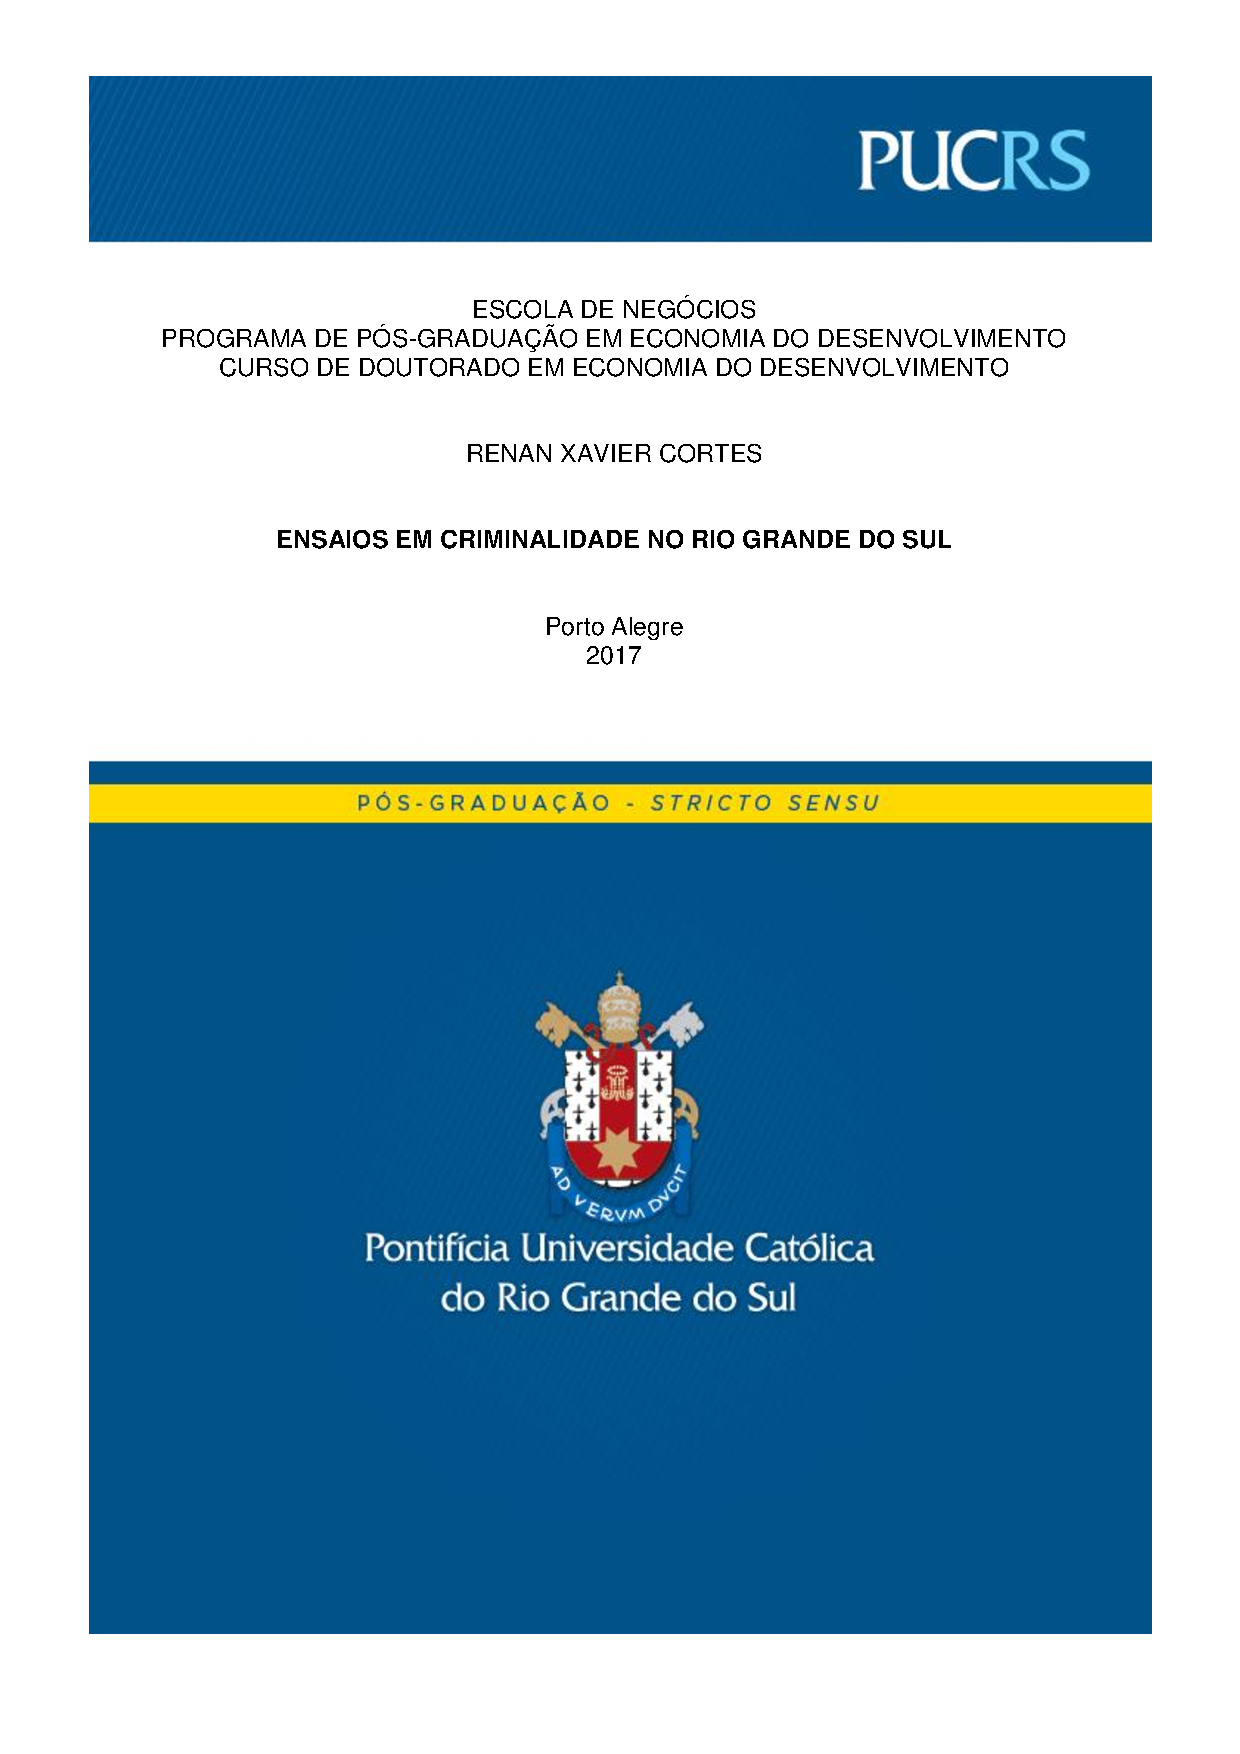
\includepdf[pages={1}]{Capa_Tese_Renan.pdf}
%\includepdf[pages={4}]{ata_aprovacao.pdf}

\Sconcordance{concordance:TESE_DE_DOUTORADO_RENAN_FINAL.tex:TESE_DE_DOUTORADO_RENAN_FINAL.Rnw:%
1 186 1 1 0 178 1 1 25 19 1 1 23 1 2 7 1 1 21 1 2 76 1 1 15 1 2 40 1 1 %
50 1 2 161 1 1 9 1 2 9 1 1 9 1 2 15 1 1 22 1 2 7 1 1 10 1 2 197 1 1 35 %
1 2 11 1 1 28 1 2 7 1 1 10 1 2 17 1 1 32 1 2 7 1 1 12 1 2 210 1 1 11 1 %
2 62 1 1 229 1 2 9 1 1 17 1 2 13 1 1 7 1 2 9 1 1 7 1 2 15 1 1 21 1 2 9 %
1 1 10 1 3 66 1 1 51 1 2 180 1 1 49 1 2 150 1 1 44 1 4 11 1 1 34 1 4 89 %
1 1 44 1 4 8 1 1 44 1 4 111 1 1 7 1 2 7 1 1 7 1 2 10 1 1 55 1 2 7 1 1 %
14 1 2 8 1 1 14 1 2 16 1 1 53 1 2 8 1 1 14 1 2 8 1 1 14 1 2 70 1 1 5 17 %
0 1 2 4 1 1 6 17 0 1 2 7 1 1 2 17 0 1 2 35 1 1 2 1 0 1 19 20 0 1 2 6 1 %
1 16 18 0 1 2 42 1 1 23 25 0 1 2 7 1 1 11 13 0 1 2 35 1 1 19 18 0 1 2 3 %
0 1 2 9 1 1 10 12 0 1 2 5 1 1 3 13 0 1 2 28 1 1 24 26 0 1 2 33 1 1 8 10 %
0 1 2 266 1 1 65 1 2 91 1 1 5 1 3 78 1 2 2 8 1 2 2 7 1 2 2 7 1 2 2 8 1 %
2 2 7 1 2 2 7 1 2 2 9 1 2 2 14 1 2 2 7 1 2 2 7 1 2 2 7 1 2 2 7 1 2 2 7 %
1 2 2 7 1 2 2 7 1 2 2 7 1 2 2 1256 1}


\frenchspacing
%\imprimircapa
\imprimirfolhaderosto*

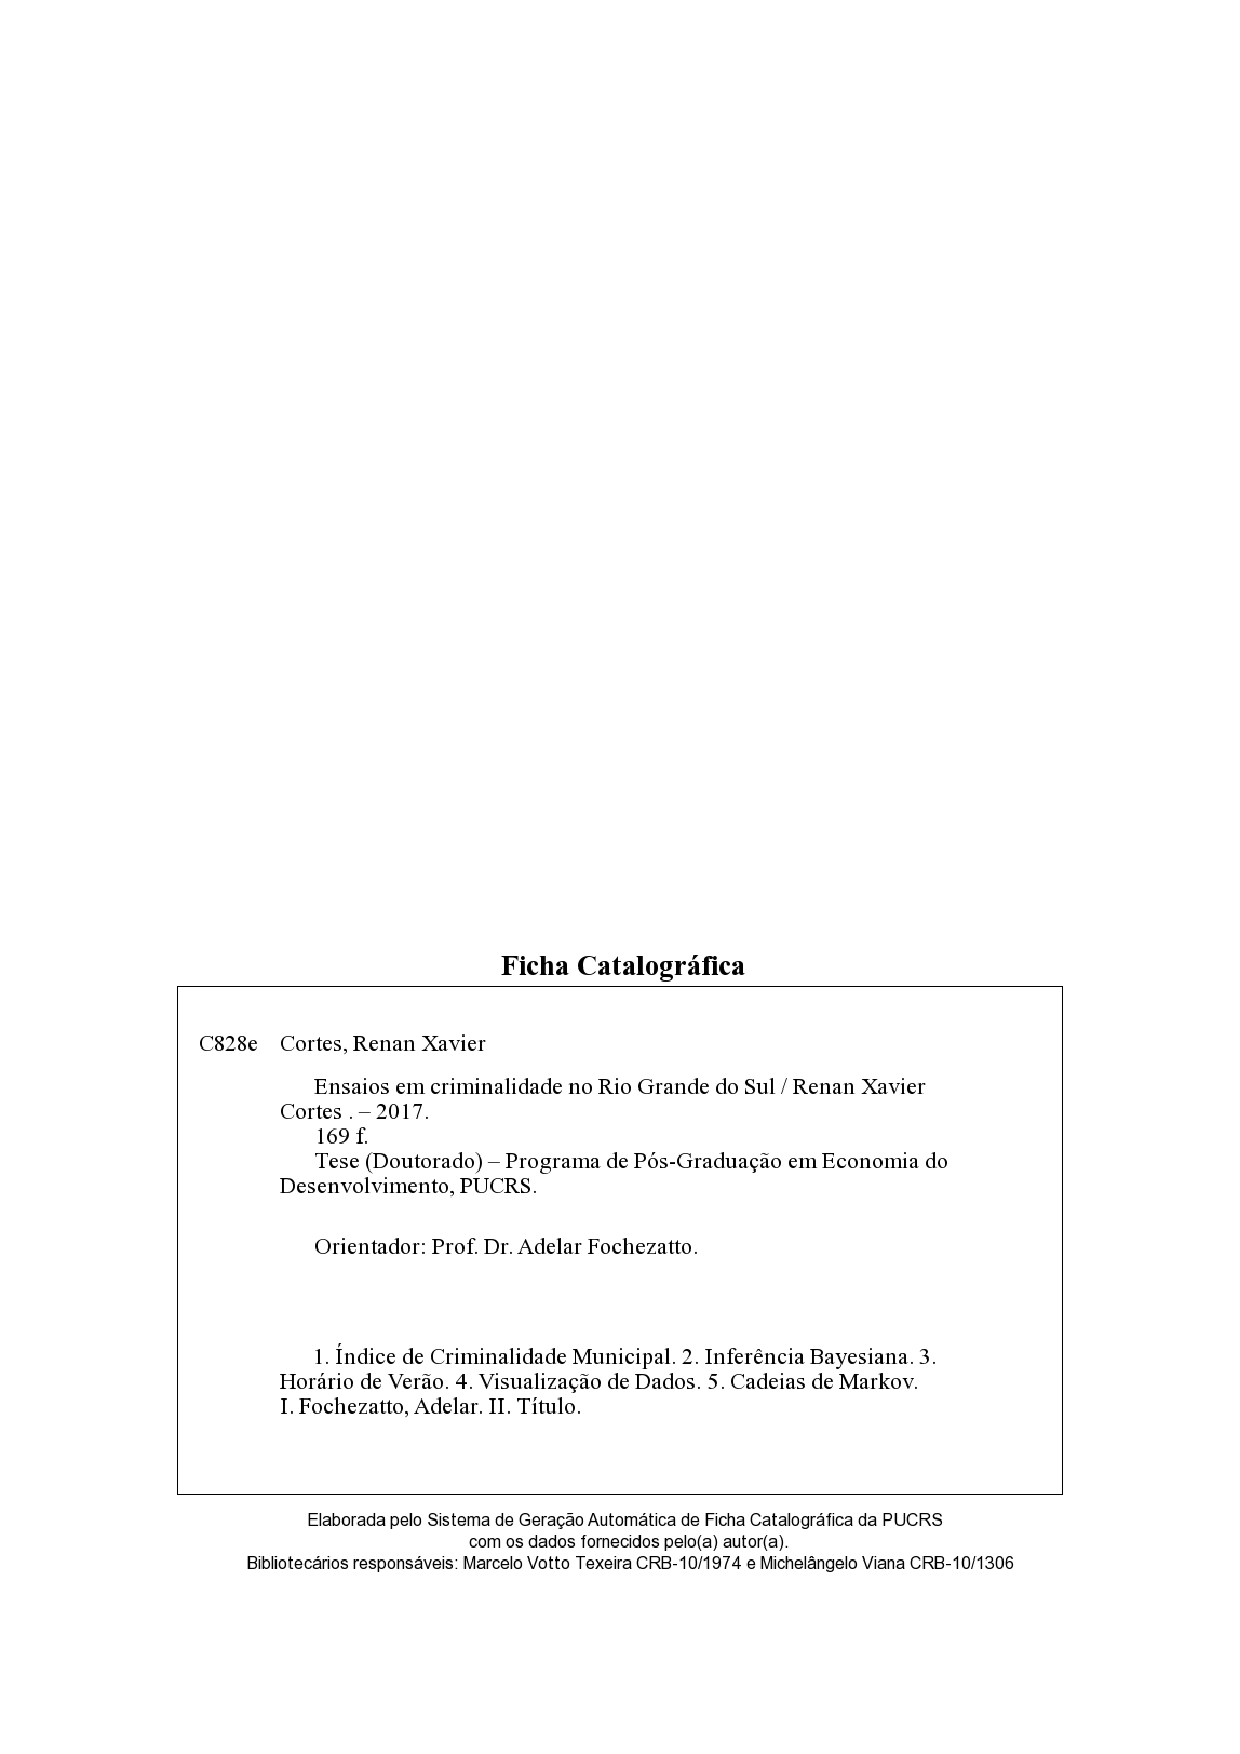
\includepdf[pages={1}]{ficha_catalografica_puc.pdf}
%\begin{fichacatalografica}
%	\vspace*{\fill}					% Posição vertical
%	\hrule							% Linha horizontal
%	\begin{center}					% Minipage Centralizado
%	\begin{minipage}[c]{12.5cm}		% Largura
%	
%	\imprimirautor
%	
%	\hspace{0.5cm} \imprimirtitulo  / \imprimirautor. --
%	\imprimirlocal, \imprimirdata-
%	
%	\hspace{0.5cm} \pageref{LastPage} p. : il. (algumas color.) ; 30 cm.\\
%	
%	\hspace{0.5cm} \imprimirorientadorRotulo~\imprimirorientador\\
%	
%	\hspace{0.5cm}
%	\parbox[t]{\textwidth}{\imprimirtipotrabalho~--~\imprimirinstituicao,
%	\imprimirdata.}\\
%	
%	\hspace{0.5cm}
%		1. Economia do Crime.
%		2. Inferência Bayesiana.
%		3. Regressão em Descontinuidade.
%		4. Visualização de Dados.
%		5. Cadeias de Markov.
%		I. Orientador: Adelar Fochezatto.
%		II. Pontifícia Universidade Católica do Rio Grande do Sul.
%		III. Programa de Pós-Graduação em Economia do Desenvolvimento.
%		IV. Ensaios em Criminalidade no Rio Grande do Sul\\ 			
%	
%	\hspace{8.75cm}\\
%	
%	\end{minipage}
%	\end{center}
%	\hrule
%\end{fichacatalografica}

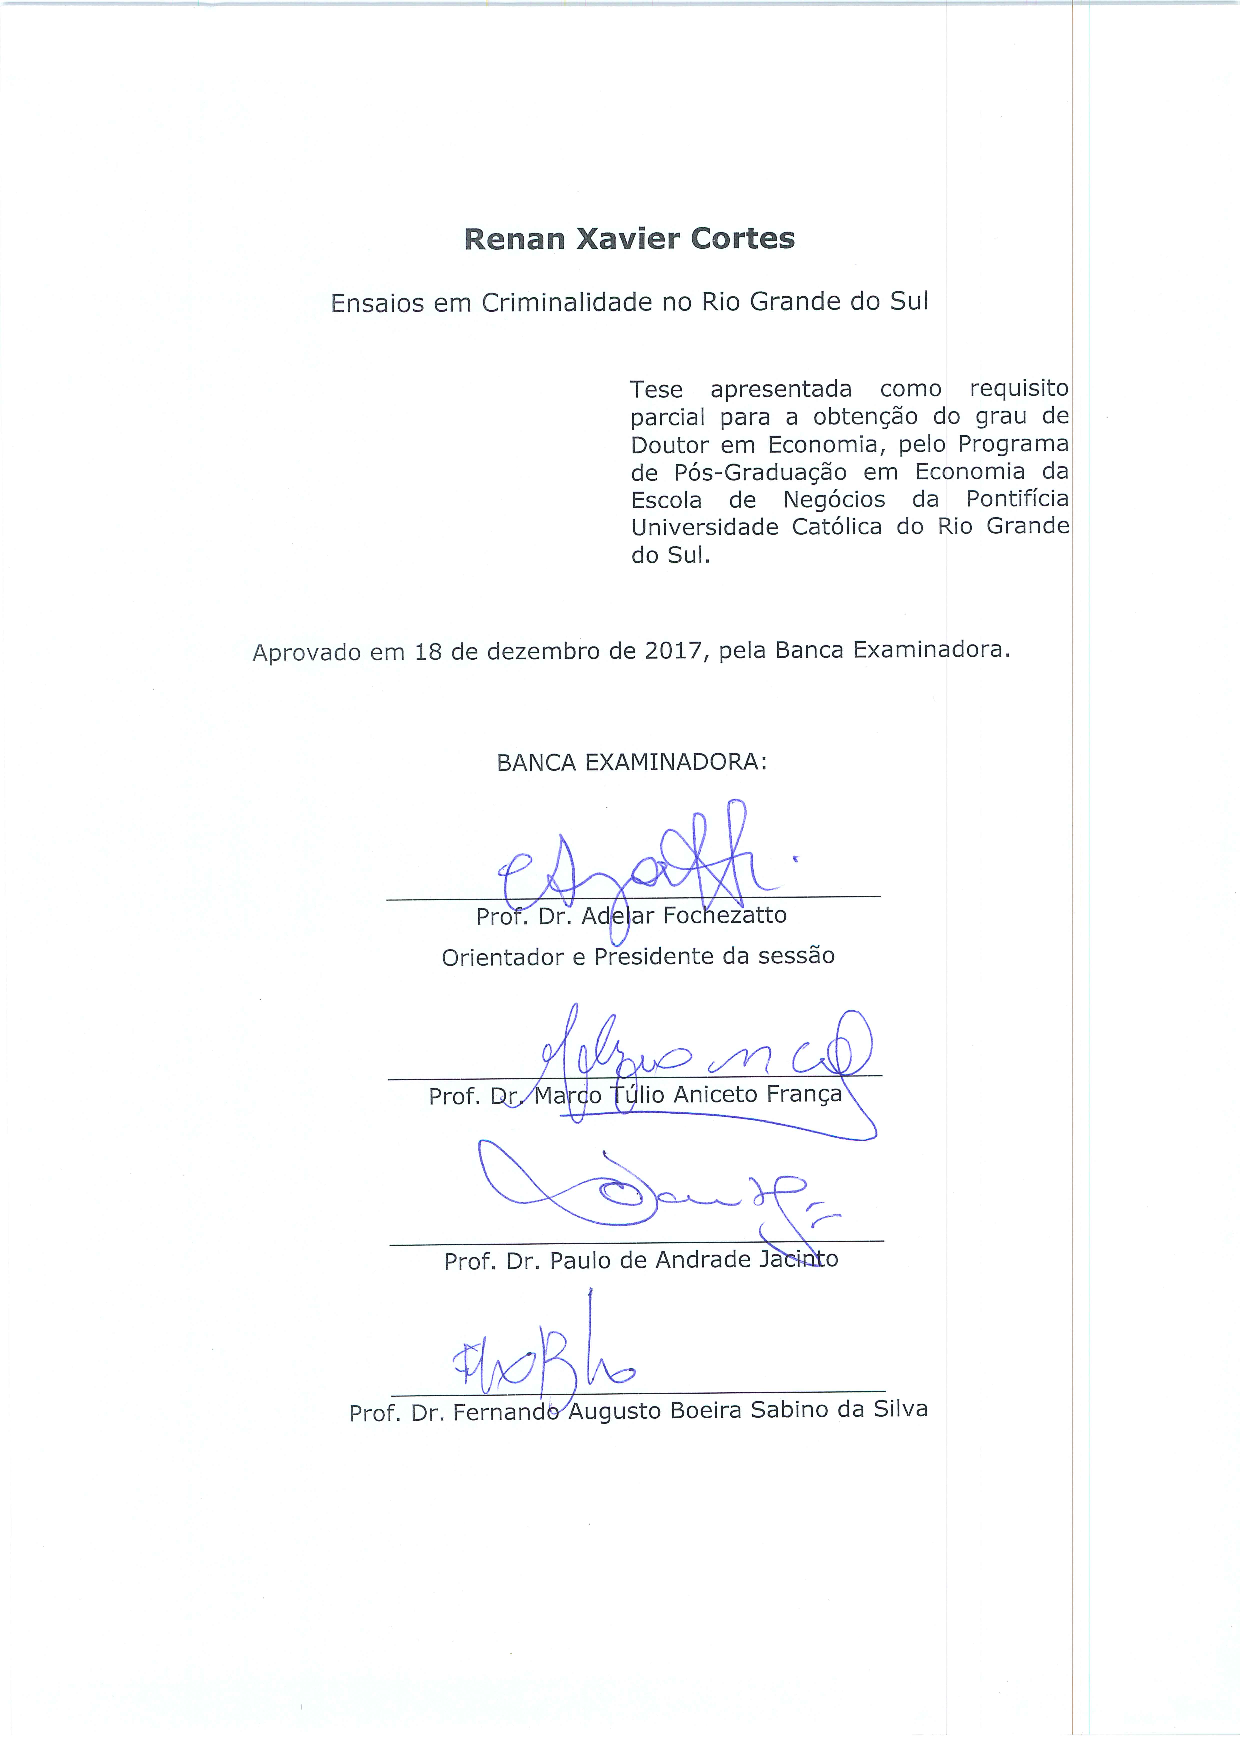
\includepdf[pages={1}]{ata_aprovacao.pdf}
%\begin{folhadeaprovacao}
%
%  \begin{center}
%    {\ABNTEXchapterfont\large\imprimirautor}
%
%    \vspace*{\fill}\vspace*{\fill}
%    {\ABNTEXchapterfont\bfseries\Large\imprimirtitulo}
%    \vspace*{\fill}
%    
%    \hspace{.45\textwidth}
%    \begin{minipage}{.5\textwidth}
%        \imprimirpreambulo
%    \end{minipage}%
%    \vspace*{\fill}
%   \end{center}
%   
%   \begin{center} \imprimirlocal, 18 de Dezembro de 2017 \\ \vspace{1cm} BANCA EXAMINADORA: %\end{center}
%
%   \assinatura{\textbf{Orientador e Presidente da Sessão} \\ Prof. Dr. Adelar Fochezatto (PUCRS)}
%   \assinatura{Prof. Dr. Paulo de Andrade Jacinto (UFPR)}
%   %\assinatura{\textbf{Professor} \\ Dr. Cristiano Aguiar de Oliveira}
%   \assinatura{Prof. Dr. Marco Túlio Aniceto França (PUCRS)}
%   \assinatura{Prof. Dr. Fernando Augusto Boeira Sabino da Silva (UFRGS)}
%   %\assinatura{\textbf{Professor} \\ Convidado 4}
%      
%   \begin{center}
%    \vspace*{0.5cm}
%    {\large\imprimirlocal}
%    \par
%    {\large\imprimirdata}
%    \vspace*{1cm}
%  \end{center}
%  
%\end{folhadeaprovacao}

% ---
% Dedicatória
% ---
%\begin{dedicatoria}
%   \vspace*{\fill}
%   \centering
%   \noindent
%   \textit{Este trabalho é dedicado à minha família,\\
%   que desde pequeno me deram todo o suporte necessário\\
%   para realizar meus objetivos.} \vspace*{\fill}
%\end{dedicatoria}
% ---

% ---
% Agradecimentos
% ---
\begin{agradecimentos}
Primeiramente, não poderia deixar de agradecer minha família que sempre deu todo o suporte necessário para eu alcançar meus objetivos. Trabalhar, fazer disciplinas e uma tese no doutorado sempre se configuraram um grande desafio de conciliação do tempo. Por muitas vezes tive que me fazer ausente devido aos compromissos acadêmicos, mas acredito que este investimento será convertido em coisas boas no futuro. 

Desde a formação do cérebro, através do leite materno, o papel da minha mãe na minha criação foi imprenscindível, além do amor e compaixão. Com relação ao meu pai, sempre presente e astuto, tive sempre muitos ensinamentos e devo a ele a carga genética voltada para a área de exatas. A parceria com meu irmão sempre foi importante ao longo desses anos. Todos vocês sempre desempenharam um papel fundamental na minha formação e eu devo tudo a vocês por ser quem eu sou. Amo todos vocês!

Em segundo lugar, agradeço imensamente a minha grande companheira Carol que me apoiou e caminhou ao meu lado durante todos os anos do meu doutorado desde a minha aprovação até o momento da defesa. Sem sombra de dúvidas, o seu companheirismo, carisma e amor trazem uma paz imensurável. Obrigado por ser essa pessoa tão especial!

Não posso deixar de agradecer também ao corpo docente do Programa de Pós-Graduação em Economia do Desenvolvimento (PPGE) da PUCRS. Tendo em vista o meu background estatístico e tendo que encarar um doutorado em economia, tive a sorte de ter grandes professores desde as disciplinas mais introdutórias quanto as mais avançadas. Em especial, agradeço imensamente ao meu orientador Adelar Fochezatto que desde a época em que o conheci como presidente da Fundação de Economia e Estatística (FEE) já se mostrava uma pessoa excepcional de fácil convivência e, acima de tudo, um excelente profissional. Muito obrigado por, gentilmente, ter aceitado a orientação e estar sempre presente lendo os artigos da tese, dando ideias, contribuindo para a evolução do trabalho, trocando e-mails e estar sempre disponível na sua sala. Devo muito desta tese a ti! Obrigado!

Agradeço também ao Paulo Jacinto que me orientou inicialmente nesta tese, mas que devido a sua mudança para incorporar o corpo docente do Programa de Pós-Graduação em Desenvolvimento Econômico da UFPR foi impossibilitado de continuar a orientação. Obrigado e boa sorte na UFPR! Além disso, agradeço aos demais membros da banca, como o Marco Túlio, que contribuiu também na minha defesa do projeto, e o Fernando Sabino, que desde a minha graduação em estatística tem sido um grande parceiro. Agradeço também ao Cristiano Oliveira por ter feito contribuições na minha defesa de projeto.

Por fim, não posso esquecer dos meus queridos amigos e colegas da FEE. Em especial, ao pessoal do Centro de Informações Estatísticas e Sociais (CIES) e ao pessoal da Assessoria da Presidência que sempre foram um espelho pra mim em termos de pesquisa acadêmica e profissional. Poderia citar diversos nomes aqui, mas deixo registrado o meu obrigado ao Pedro Zuanazzi, que foi meu colega de doutorado e de FEE, e ao Rafael Bernardini que participou da construção da base de dados do segundo ensaio desta tese.

\end{agradecimentos}


% ---
% RESUMOS
% ---

% resumo em português
\begin{resumo}

Esta tese aborda o tema da criminalidade no Rio Grande do Sul (RS) através de quatro ensaios. O primeiro se dedica a fazer uma discussão aprofundada dos crimes nos municípios gaúchos, enfatizando os problemas relacionados a estimações de taxas brutas, principalmente em municípios pequenos. Este artigo, além de fazer uma extensa análise descritiva da criminalidade municipal no RS, busca contornar os problemas de estimação fazendo uso da abordagem bayesiana \textit{Integrated Nested Laplace Approximation} (INLA) a fim de criar índices agregados de criminalidade. Utilizando as penas previstas em leis, criou-se também índices desagregados contra o patrimônio e contra a vida e a abordagem utilizada se mostrou eficiente na redução de variabilidade de municípios com alta variância. O segundo artigo avalia o efeito da luminosidade na criminalidade gaúcha estimando o efeito do horário de verão (HV). Diversas regressões em descontinuidade, tanto no período de início do HV, quanto no final, foram estimadas. Possíveis efeitos foram controlados, como o dia da semana e variáveis climatológicas, e os resultados apontam que, majoritariamente, não existe efeito significativo do HV na criminalidade do RS. Estes resultados se mostraram robustos a diferentes especificações dos modelos. O terceiro se refere a uma nova ferramenta de visualização de dados interativa das ocorrências criminais no RS, o CrimeVis. Esta plataforma de visualização é construída usando a tecnologia \textit{Shiny} e a linguagem \texttt{R} com diversos tipos de visualizações. Este artigo discute a importância da visualização de dados, exemplifica a construção do CrimeVis através de códigos e mostra como que ele se configura um dispositivo poderoso para compreensão da dinâmica criminal gaúcha. O quarto, e último, ensaio busca estudar a temporalidade e a espaço-temporalidade dos crimes no RS através de Cadeias de Markov. Este artigo estima as probabilidades de transição e razões de chance dos municípios gaúchos entre os estados de ausência/presença de crime de um período inicial em relação à presença/ausência de um período final. Ademais, o efeito conjunto espacial de vizinhança no período inicial também é medido. As evidências mostraram que existe um deslocamento de roubo de veículos para a região metropolitana de Porto Alegre e um forte efeito de vizinhança na transição mais recente 2015-2016, uma estabilidade temporal em homicídios (com esfeito espaço-temporal de vizinhança) e tráfico de entorpecentes com regiões de ocorrência definidas entre o norte e o sul do estado e uma quebra estrutural acentuada nos delitos relacionados à armas e munições entre o ano de 2003 e 2004.

 \vspace{\onelineskip}
    
 \noindent
 \textbf{Palavras-chaves}: Índice de Criminalidade Municipal. Inferência Bayesiana. Horário de Verão. Visualização de Dados. Cadeias de Markov.
\end{resumo}

% resumo em inglês
\begin{resumo}[Abstract]
 \begin{otherlanguage*}{english}
This thesis approaches the theme of crime in Rio Grande do Sul (RS) through four essays. The first one is devoted to an in-depth discussion of crimes in the municipalities of Rio Grande do Sul, emphasizing the problems related to the raw rates estimations, especially in small municipalities. This article, in addition to making an extensive descriptive analysis of municipal crime in RS, seeks to overcome the problems of estimation by using the bayesian Integrated Nested Laplace Approximation (INLA) approach to create aggregate crime rates. Using the law penalties for each crime type, we also created disaggregated indexes against economic patrimony and against life and the approach used was efficient in reducing the variability of municipalities with high volatility. The second article assess the effect of luminosity on RS crimes, estimating the effect of the Daylight Savnig Time (DST). Several discontinuous regressions, both at the beggining of DST and at the end, were estimated. Possible effects were controlled, as weekday and climatological variables, and the results indicate that, mostly, there is no significant effect of DST on RS crimes. These results were robust to different model specifications. The third refers to a new tool for interactive data visualization of criminal occurrences in RS, CrimeVis. This visualization platform is constructed using \textit{Shiny} technology and the \texttt{R} language with several types of visualizations. This article discusses the importance of data visualization, exemplifies the construction of CrimeVis through codes and shows how it is a powerful device for understanding the criminal dynamics of RS. The fourth, and last, essay seeks to study the temporality and space-temporality of crimes in RS through Markov Chains. This article estimates the transition probabilities and odds ratios of municipalities between absence/presence of crime of an initial period in relation to a presence/absence of a final period. In addition, the spatial neighborhood joint effect of the initial period is also measured. Evidence has shown that there is a displacement of cars robbery to the metropolitan region of Porto Alegre and a strong neighborhood effect in the most recent transition from 2015-2016, a temporal stability in homicides (with space-time neighborhood effects) and narcotics trafficking with defined regions of occurrence between the north and the south of the state and a highlighted structural break in the crimes related to the arms and ammunition between the year of 2003 and 2004.



 \vspace{\onelineskip}

 \noindent 
 \textbf{Keywords}: Municipal Crime Index. Bayesian Inference. Daylight Saving Time. Data Visualization. Markov Chains.
 \end{otherlanguage*}
\end{resumo}

% ---
% inserir lista de ilustrações
% ---
\setlength{\cftfigurenumwidth}{15mm} % Para dar um espaço entre o número e a descrição da figura na lista de figuras
\pdfbookmark[0]{\listfigurename}{lof}
\listoffigures*
\cleardoublepage
% ---

% ---
% inserir lista de tabelas
% ---
\setlength{\cfttablenumwidth}{15mm} % Para dar um espaço entre o número e a descrição da tabela na lista de tabelas
\pdfbookmark[0]{\listtablename}{lot}
\listoftables*
\cleardoublepage
% ---

% ---
% inserir o sumario
% ---
\pdfbookmark[0]{\contentsname}{toc}
\tableofcontents*
\cleardoublepage
% ---



% ----------------------------------------------------------
% ELEMENTOS TEXTUAIS
% ----------------------------------------------------------
\textual






% ----------------------------------------------------------
% Introdução
% ----------------------------------------------------------
\chapter{Introdução\label{chap:Introducao}}

A criminalidade afeta direta ou indiretamente a vida das pessoas. Provavelmente, a maior parte dos brasileiros já foi vítima de algum delito ou conhece algum amigo ou parente que foi. Em termos de homicídio, o Brasil teve em 2015 uma taxa de homicídios de 28,9 a cada 100 mil habitantes, representando um aumento de 10,6\% desde 2005. Em valores brutos, houve 59.080 homicídios. No Rio Grande do Sul (RS), esta taxa partiu de 15,1 em 2002 para 23,3 em 2016, um aumento de 54,1\%,  totalizando 2.627 ocorrências de homicídio doloso, segundo dados da Secretaria de Segurança Pública do RS.

Com relação às taxas de homicídios cometidos por armas de fogo (HAF), segundo \co{waiselfisz2016mapa}, o RS ocupava a décima primeira posição entre as unidades federativas brasileiras em 2000, com um valor de 16,3. Esta posição passou a ser a décima nona no ano de 2014 com 18,7. Segundo este mesmo estudo, o estado brasileiro que liderou o ranking em 2014, foi Alagoas com 56,1, seguido pelo Ceará com 42,9, Sergipe com 41,2 e Rio Grande do Norte com 38,9. Em termos internacionais, segundo o Instituto Igarapé, o Brasil ocupa a quarta colocação no ranking de homicídios por 100 mil habitantes, logo atrás de Honduras, México e El Salvador. A capital gaúcha, Porto Alegre, figurou entre as 50 cidades mais violentas do mundo em 2016.

A forte crise nacional que se iniciou em 2014 desencadeou uma grave crise fiscal que vem assolando algumas unidades da federação. Especificamente, o governo do RS teve dificuldades em honrar em dia os pagamentos dos servidores do executivo o que implicou em uma greve de membros da segurança pública estadual no ano de 2015\footnote{http://g1.globo.com/rs/rio-grande-do-sul/noticia/2015/09/no-4-dia-de-greve-no-rs-familiares-de-pms-trancam-saida-de-batalhoes.html}, o que aumentou a sensação de insegurança na população gaúcha. Complementarmente, há insuficiência de efetivos, o que culminou no deslocamento de membros da força nacional em agosto de 2016\footnote{https://g1.globo.com/rs/rio-grande-do-sul/noticia/governo-pede-permanencia-da-forca-nacional-de-seguranca-no-rio-grande-do-sul-em-2018.ghtml}.

Não obstante, além da recessão e da crise financeira vivida nos recentes anos pelo RS, houve também um aumento acentuado da taxa de desemprego na sua região metropolitana, o que também pode ter influência nas taxas de homicídio \cite{cerqueira2015efeito}. As Figuras \ref{fig:pib_int} e \ref{fig:desem_int} mostram, respectivamente, a evolução do PIB trimestral gaúcho, que apresentou queda a partir do quarto trimestre de 2014, e a taxa de desemprego na Região Metropolitana de Porto Alegre (RMPA) que teve um aumento acentuado no início de 2015. Nestes gráficos podemos analisar dois comportamentos. Primeiramente, o PIB partiu de 1,7\% no terceiro trimestre de 2014, passando por -2\% no primeiro trimestre de 2015 e chegando ao ponto mínimo de -5,5\% no segundo trimestre de 2016. Em segundo lugar, a taxa de desemprego que estava em 5,7\% em janeiro de 2015 aumentou bruscamente chegando ao valor de 12\% em outubro de 2017.

\begin{figure}[H]
\begin{center}
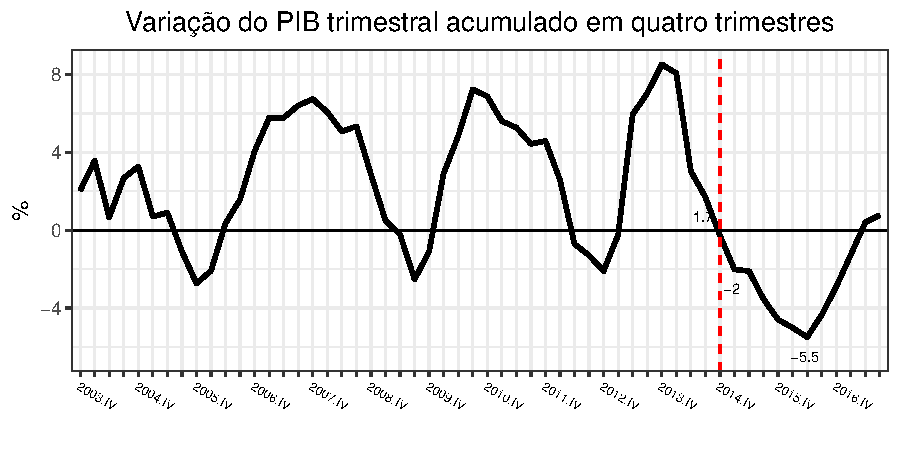
\includegraphics{TESE_DE_DOUTORADO_RENAN_FINAL-plot_pib_introducao}
\end{center}
\caption{Variação do PIB trimestral gaúcho acumulado em quatro trimestres — 2003/IV-2017/III (em \%)}
\source{Fonte: FEE-RS.}
\label{fig:pib_int}
\end{figure}

\begin{figure}[H]
\begin{center}
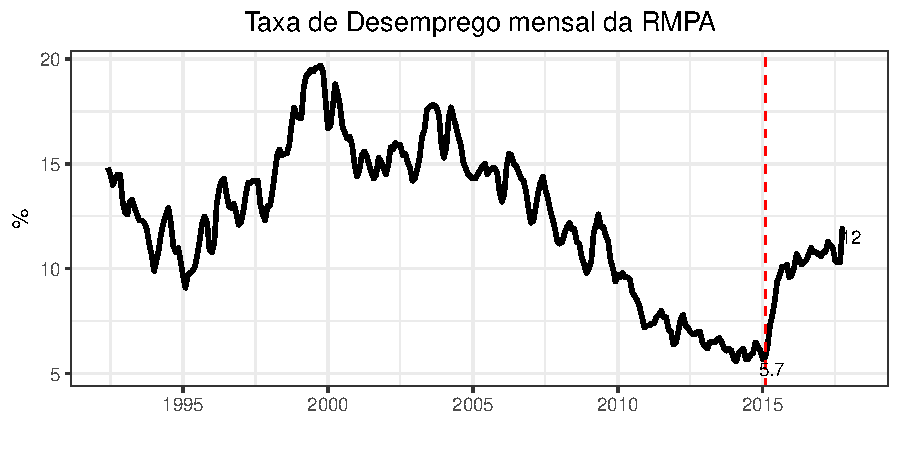
\includegraphics{TESE_DE_DOUTORADO_RENAN_FINAL-plot_desem_introducao}
\end{center}
\caption{Taxa de Desemprego mensal da RMPA — 1992/Jun.-2017/Out. (em \%)}
\source{Fonte: PED-FEE.}
\label{fig:desem_int}
\end{figure}

Tendo em vista os pontos levantados que chamam a atenção para o caso específico do RS e combinado ao fato de que o autor deste trabalho é pesquisador da fundação pública estadual Fundação de Economia e Estatística Siegfried Emanuel Heuser (FEE-RS)\footnote{https://www.fee.rs.gov.br/} do Rio Grande do Sul, a presente tese aborda a questão da criminalidade especificamente para o caso desta unidade da federação e é composta por quatro ensaios. Em cada um dos trabalhos, diferentes temas são abordados. 

O primeiro ensaio utiliza os diferentes tipos de crimes nos municípios do Rio Grande do Sul a fim de criar um índice geral de criminalidade. Através de recentes métodos de estimação bayesiana, foi de interesse contornar conhecidos problemas na literatura de excesso de variabilidade em regiões pequenas. Além disso, fazendo uso das penas criminais, criou-se um índice geral de criminalidade que possui uma interpretação simples e com alto grau de comunicabilidade.

O segundo ensaio analisa o efeito da claridade do ambiente no comportamento criminal estimando o efeito do horário de verão sobre a criminalidade no Rio Grande do Sul. Foi de interesse avaliar se existe descontinuidade nas taxas de homicídios gaúchas quando se inicia e quando finda a política brasileira do horário de verão.

A plataforma de visualização de dados de criminalidade CrimeVis é o tema do terceiro ensaio. Neste trabalho, é apresentada a construção de cada um dos componentes deste aplicativo, que faz uso da tecnologia \textit{Shiny}, mostrando como que esta ferramenta pode auxiliar na compreensão da dinâmica criminal gaúcha.

O quarto e último ensaio desta tese se dedica a estudar a dinâmica temporal e espaço-temporal dos crimes no RS através de cadeias de Markov, razões de chance de probabilidades de transições e testes de homogeneidade temporal e espaço-temporal. O objetivo é verificar se as regiões tendem a apresentar mudanças de criminalidade em período final comparativamente a um período inicial. Ademais, o fator espacial, mensurado através da presença criminal em municípios vizinhos, também é avaliado conjuntamente. Neste ensaio, também apresentam-se estas novas funcionalidades na ferramenta CrimeVis.










\chapter{Crimes nos municípios gaúchos: análise a partir de um índice geral de criminalidade\label{chap:indice}}

\section{Introdução\label{sec:Introdução_Indice}}

O objetivo deste artigo é fazer um estudo sobre crimes e propor um índice de criminalidade municipal do Rio Grande do Sul para englobar diferentes características e tentar evitar possíveis problemas de estimação. Quais são as regiões mais perigosas? Quais são os municípios com os maiores índices de criminalidade? Estas são perguntas que constantemente são levantadas quando se deseja comparar unidades geográficas. 

A criminalidade, bem como a sensação de insegurança, diminui o bem-estar da população residente de um determinado local, pois este fenômeno interpessoal afeta diretamente o modo como as pessoas vivem e se relacionam. Ela gera mudanças de hábitos usuais e de escolhas, tais como modificações de meios de transporte, privações de consumo de lazer, gastos com segurança particular, modificações de locais de residência, preço de imóveis (conforme estudado em \co{frischtak2012fedny}), entre outros, o que provoca uma forte demanda por parte da população no combate ao crime. Os agentes econômicos envolvidos necessitam alocar esforços a fim de diminuir ao máximo a incidência de crime em determinado espaço e tempo e, neste sentido, o estudo apronfundado da criminalidade, em especial no avanço de métodos de mensuração deste fenômeno, se justificam cada vez mais.

Segundo os registros de boletins de ocorrência da Secretaria de Segurança Pública do Rio Grande do Sul e estimativas populacionais da Fundação de Economia e Estatística, no estado do Rio Grande do Sul entre 2002 e 2015 aumentaram o número de homicídios dolosos em 53,7\%, de latrocínios em 28,4\%, de roubos em 47,1\%, de roubos de veículos em 116,5\% e de furtos de veículos em 8,7\%, enquanto que a população cresceu 7,5\%. Conforme \co{monteiro2009mono} e \co{cortes2016tdfee}, a maior parte das taxas criminais de ocorrência são concentradas em municípios mais populosos, em especial, na região metropolitana de Porto Alegre e em municípios litorâneos. No entanto, estes rankings municipais de criminalidade podem variar substancialmente dependendo do tipo de crime que se está analisando e, além disso, a queda do bem-estar da potencial vítima ou o ''efeito trauma'' da vítima também varia de acordo com a gravidade da atividade criminosa. Por exemplo, é razoável supor que uma pessoa que teve seu carro furtado experienciou um evento menos traumático do que  uma vítima que teve seu carro roubado\footnote{O furto se caracteriza como a subtração do bem sem o contato direto com a vítima, enquanto que o roubo é caracterizado como um crime mais grave, pois o delinquente coage a vítima a entregar o bem mediante ameaça ou emprego de violência.}.

Para se trabalhar com indicadores de criminalidade uma série de problemas devem ser observados como se dicute em \co{khan2005manual}, \co{justus2012EconomiA} e \co{cerqueira2005mito}. \co{khan2005manual} analisa estes pontos argumentando que os dados oficiais de criminalidade estão sujeitos a uma série de limites de validade e confiabilidade, pois são antes um retrato do processo social de notificação de crimes do que um retrato fiel do universo dos crimes realmente cometidos num determinado local, uma vez que para um crime ir para as estatísticas oficiais ele deve ser detectado, notificado e registrado. Algumas das especificidades a serem levantadas são a sazonalidade criminal, a subnotificação\footnote{\co{khan2005manual} mostra que Pesquisas de Vitimização sugerem que, em média, apenas um terço dos crimes são notificados.}, a concentração em pequenos locais, a propensão da vítima a notificar o crime (que pode variar de acordo com a percepção com relação ao sistema policial, tipo de crime ou bem roubado) e a simultaneidade entre ação policial e notificação.

Um dos problemas mais conhecidos na literatura sobre o tema é como fazer uma boa estimação do número de ocorrências criminais em municípios pequenos. Este problema advém, basicamente, por dois fatores: a alta variância que um município pequeno pode apresentar nas suas taxas brutas de criminalidade e a alta probabilidade de não se observar algum evento em um dado período de tempo. Com relação à primeira questão, pode-se pensar que é possível que um evento atípico em um determinado município pouco populoso aumente severamente as taxas criminais que, usualmente, são apresentadas em termos de 100.000 habitantes. \co{carvalho2012saude} verificou que em 2008 a taxa de homicídio de Nova Marilândia (MT) foi de 211,1 o que representa um valor mais de 3 vezes maior do que a do país com maior taxa de homicídio do mundo\footnote{Segundo \co{Waiselfisz2014}, o país que apresentou a maior taxa, em 2009, foi El Salvador com 62,4 homicídios por 100.000 habitantes.}. No entanto, este município apresentou apenas cinco homicídios tendo apenas 2.369 habitantes. 

Com relação à segunda questão, a sua pertinência se deve ao fato de que mesmo em uma cidade que não teve nenhum caso de crime em determinado ano, não necessariamente a probabilidade de ele acontecer seja nula, pois, na realidade, não foi observada uma janela de tempo suficiente para ele acontecer. Este fenômeno, que também abrange o campo epidemiológico, já possui uma ampla discussão e difusão na literatura, podendo-se citar \co{clayton1987biometrics}, \co{marshall1991journalserieC}, \co{pringle1996ecosoc} e \co{catelan2010biomj}. 

A maior parte das metodologias tentam remediar o problema estabelecendo estimativas bayesianas que podem levar em consideração a estrutura espacial para suavizar as estimativas brutas. \co{carvalho2012saude} analisam diferentes métodos de estimação para taxas de homicídio para os municípios brasileiros comparando taxas brutas, espaciais, bayesianas empíricas, bayesianas empíricas espaciais e a taxa bayesiana de \co{clayton1987biometrics}. Tendo em vista o escopo nacional do trabalho não é aconselhado a aplicação da taxa bayesiana empírica, pois a correção foi feita com base na média do país. As melhores taxas que se adaptaram foram as bayesianas empíricas, empírica espacial e a de \co{clayton1987biometrics} com a ressalva da alta sensibilidade frente às distribuições \textit{a priori}.

Além destas questões que envolvem a qualidade dos registros criminais e problemas de estimação, é preciso também levantar outros pontos pertinentes para se criar um índice geral que combine diferentes tipos de crime. Neste sentido, \co{freitas2016xixeeg} propuseram um índice geral de criminalidade para os municípios gaúchos fazendo uso da estimação empírica bayesiana de acordo com a similaridade dos municípios e combinando os crimes ponderando-os de acordo com a pena prevista no Código Penal Brasileiro para o ano de 2013. Neste trabalho, ocorrências de 14 crimes disponibilizados pela SSP-RS foram analisados e combinados. Uma limitação deste estudo foi não discernir de maneira satisfatória os municípios gaúchos com população pequena, o que pode ter comprometido o resultado final do índice e o seu uso não evidenciar a real situação do município. No âmbito do Rio Grande do Sul, \co{cortes2016tdfee} fez uso de técnicas estatísticas multivariadas combinando componentes principais e análise fatorial a fim de encontrar uma combinação linear satisfatória de 14 crimes para o ano de 2014 para a criação de um índice municipal sem levar em consideração a gravidade penal. Algo similar foi feito também por \co{monteiro2009mono}, enquanto que a gravidade penal também foi utilizada em \co{saravia2016cedeplar}.

A abordagem \textit{Integrated Nested Laplace Approximation} (doravante referida como INLA) é uma recente abordagem de estimação Bayesiana para uma ampla classe de modelos. Introduzida por \co{rue2009approximate}, esta metodologia se destaca perante às abordagens usuais de inferência bayesiana, tendo em vista que ela permite computar de maneira rápida as estimativas das distribuições marginais \textit{a posteriori} sem necessitar de simulações estocásticas tais como os métodos MCMC \cite{gelfand1990sampling} ou \textit{Gibbs Sampling} \cite{geman1984gibbs}, pois ela trabalha com aproximações analíticas destas distribuições. Além disso, conforme \co{cortes2014dissertacao}, devido a sua natureza de aproximação analítica, o INLA não sofre dos conhecidos problemas de convergência dos métodos MCMC discutidos, por exemplo, em \co{gelman1992}, \co{raftery1992} e \co{gamerman2006markov}.

Vale destacar aqui as vantagens do indicador proposto neste ensaio uma vez que ele possui características únicas na literatura. Além da abordagem INLA utilizada, o que permite englobar efeitos espaciais e temporais de maneira rápida e eficiente em um modelo bayesiano, será de interesse também estimar o índice para diferentes classes de crimes, a saber, contra a vida e contra o patrimônio. Neste sentido, diferentes utilizações para ele podem ser dadas dependendo da ótica da análise. Por exemplo, uma seguradora pode querer precificar seus serviços de acordo com uma medida de criminalidade contra o patrimônio de uma determinada região, enquanto que o gestor público pode ter um interesse maior em reduzir o número de mortes devido à criminalidade. Ademais, uma grande vantagem do indicador é a interpretabilidade e comunicabilidade do seu valor, ao invés de simplesmente sumarizar o grau criminal numa escala que não possui interpretação prática como, por exemplo, entre 0 e 1 como em \co{freitas2016xixeeg}. Veremos que o índice aqui proposto representa quanto tempo cada pessoa teria que passar presa para pagar por todos os crimes de seu município.

A partir dessas considerações, o presente estudo tem como objetivo, construir um índice para a criminalidade municipal no RS fazendo uso de métodos frequentistas e bayesianos espaciais para a estimação das prevalências de cada crime. Para tanto será feito uso dos modelos bayesianos, utilizando a abordagem INLA \cite{rue2009approximate,martino2009implementing} disponível no pacote \texttt{inla} do software \texttt{R}\footnote{https://www.r-project.org/}, até então com uso inédito para esta finalidade. As estimativas criminais que melhor se adaptarem aos dados serão utilizadas para a construção do índice geral de criminalidade proposto.

\section{Metodologia\label{sec:Metodologia_Indice}}

Esta seção apresenta a metodologia empregada na construção do índice de criminalidade. Para tanto, inicialmente descrevem-se as medidas usadas para estimar as taxas de criminalidade, na sequência, apresentam-se os conceitos de matrizes de vizinhança, índice I de Moran, modelos autoregressivos condicionais, a abordagem INLA, a descrição da base de dados utilizada e a combinação dos crimes. 

Uma das opções de se estimar a prevalência de uma atividade criminosa pode ser dada pela Taxa Bruta ($TB$), por 100.000 habitantes, de ocorrência dada pela seguinte equação:
\begin{align}
TB_{i}=\frac{Y_i}{P_i}\times100.000, \ i=1,...,n
\end{align}
onde $Y_i$ representa o número de casos observados da região $i$, $P_i$ representa a população da região $i$ e $n$ o número de unidades geográficas sob estudo. No entanto, conforme já discutido, este tipo de abordagem sofre de diversos problemas tanto em termos de subestimação, quanto em termos de variabilidade, principalmente em unidades geográficas pouco populosas. Uma das opções para evitar este tipo de problema é utilizar a taxa bayesiana empírica proposta por \co{marshall1991journalserieC}, utilizada também em \co{carvalho2012saude} e em \co{cerqueira2013brasilemdesen}. Esta taxa considera a variável $Y_i$ como seguindo uma distribuição de Poisson com parâmetro $P_i\times \lambda_i$, ou seja, $Y_i|P_i,\lambda_i \sim Poisson(P_i\times \lambda_i)$. No entanto, em \co{marshall1991journalserieC} a estimativa de $\lambda_i$ é muito simples representando apenas uma espécie de média ponderada entre a taxa bruta e a taxa global de eventos de toda a região sob estudo da seguinte forma:
\begin{align}
\widehat{\lambda_i} = w_i\times TB_i + (1 - w_i)\times m
\end{align}
em que $TB_i$ é a taxa bruta da região $i$, $m$ é a taxa global dos eventos (por exemplo, a taxa global do Rio Grande do Sul) e $w_i$ é um peso que é diretamente relacionado com o tamanho da população da área $i$. Sendo assim, $P_i\uparrow\Rightarrow w_i\rightarrow 1 \Rightarrow \widehat{\lambda_i} \approx  TB_i$, ou seja, a medida que o município tem população cada vez maior, mais a taxa bruta se aproxima da bayesiana empírica. O nome \textit{empírica} vem do fato que a distribuição \textit{a priori} do parâmetro desconhecido $\lambda_i$ é estimada diretamente fazendo uso dos dados sob análise. 

Os métodos empregados aqui se diferem uma vez que as abordagens farão uso da estrutura espacial de cada uma das unidades observacionais, bem como investigará diferentes estruturas de especificações, estimando os métodos tanto de maneira frequentista, quanto de maneira bayesiana\footnote{Uma boa literatura sobre o tema de estatística e econometria espacial pode ser encontrada em \co{besag1974}, \co{lesage1997irsr}, \co{lesage1999econometrics}, \co{banerjee2004hierarchical} e \co{bivand2008spatialwithR}}.

\subsection{Matrizes de Vizinhança\label{subsec:Matrizes_Indice}}

Modelos econométricos espaciais levam em consideração a relação da vizinhança entre as observações. Dados em séries temporais também possuem uma estrutura estabelecida de relacionamento, uma vez que os dados podem ser ordenados. No entanto, para dados espaciais não faz sentido uma ordenação, mas sim a definição de uma estrutura de relacionamento associada aos dados que indique a vizinhança de cada uma das unidades geográficas.

A estrutura de vizinhança pode ser representada por uma matriz de adjacência $\mathbf{A}$, associada, que é uma matriz cujo elemento $\mathbf{A}_{i,j}$ é 1 se a área $i$ é vizinha da área $j$ e 0, caso contrário. A matriz $\mathbf{A}$, que também pode ser referida como grafo estruturado, é simétrica e possui zeros na sua diagonal principal, ou seja, $\mathbf{A}_{i,i}=0, i=1,...n$.

Como ilustração, suponha o seguinte mapa de alguns municípios do Rio Grande do Sul na Figura \ref{fig:rmpa}.

\begin{figure}[H]
\begin{center}
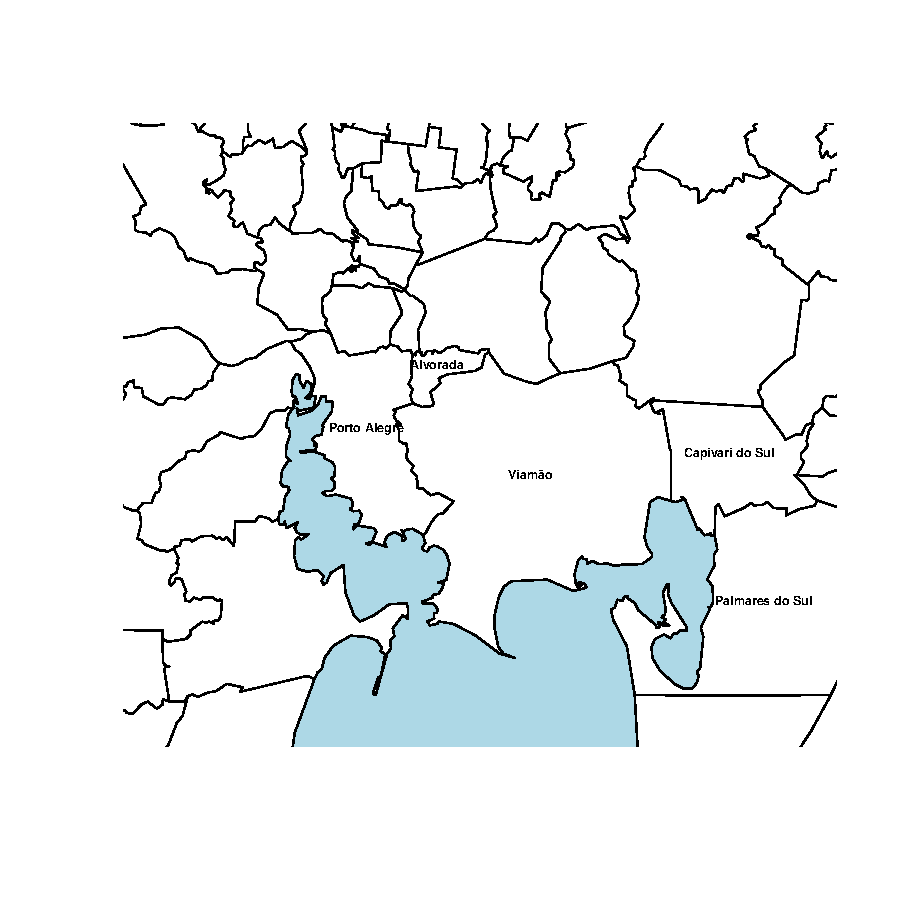
\includegraphics{TESE_DE_DOUTORADO_RENAN_FINAL-plot1}
\end{center}
\caption{Exemplo de Vizinhança de cinco municípios}
\label{fig:rmpa}
\end{figure}

Na Figura \ref{fig:rmpa}, vemos cinco municípios do Rio Grande do Sul, a saber, a capital Porto Alegre, Alvorada, Viamão, Capivari do Sul e Palmares do Sul. Poderíamos representar a estrutura espacial destas cinco cidades de acordo com os vizinhos de primeira ordem de contiguidade, isto é, com os municípios que fazem fronteira com a seguinte matriz $\mathbf{A}$ de representação:

\begin{table}[H]
\centering
\caption{Exemplo de Matriz de Vizinhança}
\label{tab:matriz_vizinhanca}
\begin{tabular}{lccccc}
                                     & Porto Alegre           & Alvorada               & Viamão                 & Capivari do Sul        & Palmares do Sul        \\ \cline{2-6} 
\multicolumn{1}{l|}{Porto Alegre}    & \multicolumn{1}{c|}{0} & \multicolumn{1}{c|}{1} & \multicolumn{1}{c|}{1} & \multicolumn{1}{c|}{0} & \multicolumn{1}{c|}{0} \\ \cline{2-6} 
\multicolumn{1}{l|}{Alvorada}        & \multicolumn{1}{c|}{1} & \multicolumn{1}{c|}{0} & \multicolumn{1}{c|}{1} & \multicolumn{1}{c|}{0} & \multicolumn{1}{c|}{0} \\ \cline{2-6} 
\multicolumn{1}{l|}{Viamão}          & \multicolumn{1}{c|}{1} & \multicolumn{1}{c|}{1} & \multicolumn{1}{c|}{0} & \multicolumn{1}{c|}{1} & \multicolumn{1}{c|}{0} \\ \cline{2-6} 
\multicolumn{1}{l|}{Capivari do Sul} & \multicolumn{1}{c|}{0} & \multicolumn{1}{c|}{0} & \multicolumn{1}{c|}{1} & \multicolumn{1}{c|}{0} & \multicolumn{1}{c|}{1} \\ \cline{2-6} 
\multicolumn{1}{l|}{Palmares do Sul} & \multicolumn{1}{c|}{0} & \multicolumn{1}{c|}{0} & \multicolumn{1}{c|}{0} & \multicolumn{1}{c|}{1} & \multicolumn{1}{c|}{0} \\ \cline{2-6} 
\end{tabular}
\end{table}

Uma das características que podemos observar é a de que, dependendo da especificação, esta matriz facilmente se torna esparsa\footnote{A esparsidade é uma característica de uma matriz que tem muitos valores zero.}. Além disto, é comum também em Econometria espacial especificar a matriz de vizinhança de forma padronizada $\mathbf{W}^{p}$. Nesta especificação, os valores de entrada são divididos pela soma da linha de forma que a soma da linha da matriz $\mathbf{W}^{p}$ é 1. Desta forma, a representação padronizada da Tabela \ref{tab:matriz_vizinhanca} ilustra as modificações a serem adotadas. Neste trabalho, as duas especificações de matrizes serão levadas em consideração.

\begin{table}[H]
\centering
\caption{Exemplo de Matriz de Vizinhança Padronizada}
\label{tab:matriz_vizinhanca_pad}
\begin{tabular}{llllll}
                                     & Porto Alegre           & Alvorada               & Viamão                 & Capivari do Sul        & Palmares do Sul        \\ \cline{2-6} 
\multicolumn{1}{c|}{Porto Alegre}    & \multicolumn{1}{c|}{0} & \multicolumn{1}{c|}{1/2} & \multicolumn{1}{c|}{1/2} & \multicolumn{1}{c|}{0} & \multicolumn{1}{c|}{0} \\ \cline{2-6} 
\multicolumn{1}{c|}{Alvorada}        & \multicolumn{1}{c|}{1/2} & \multicolumn{1}{c|}{0} & \multicolumn{1}{c|}{1/2} & \multicolumn{1}{c|}{0} & \multicolumn{1}{c|}{0} \\ \cline{2-6} 
\multicolumn{1}{c|}{Viamão}          & \multicolumn{1}{c|}{1/3} & \multicolumn{1}{c|}{1/3} & \multicolumn{1}{c|}{0} & \multicolumn{1}{c|}{1/3} & \multicolumn{1}{c|}{0} \\ \cline{2-6} 
\multicolumn{1}{c|}{Capivari do Sul} & \multicolumn{1}{c|}{0} & \multicolumn{1}{c|}{0} & \multicolumn{1}{c|}{1/2} & \multicolumn{1}{c|}{0} & \multicolumn{1}{c|}{1/2} \\ \cline{2-6} 
\multicolumn{1}{c|}{Palmares do Sul} & \multicolumn{1}{c|}{0} & \multicolumn{1}{c|}{0} & \multicolumn{1}{c|}{0} & \multicolumn{1}{c|}{1} & \multicolumn{1}{c|}{0} \\ \cline{2-6} 
\end{tabular}
\end{table}

Com relação às estruturas de vizinhança utilizadas, também denominadas de grafos, diferentes maneiras podem ser estabelecidas. Uma delas é por vizinhos de contiguidade conforme explicado anteriormente, mas uma especificação diferente pode ser por vizinhos mais próximos através da distância dos centróides de cada uma das suas localizações. Esta especificação é chamada de vizinho mais próximo de k-ésima ordem ou k-NN (do inglês, \textit{k nearest neighbor}) e, neste trabalho, testou-se até o vizinho mais próximo de terceira ordem conforme a Figura \ref{fig:especif}.

\begin{figure}[H]
\begin{center}
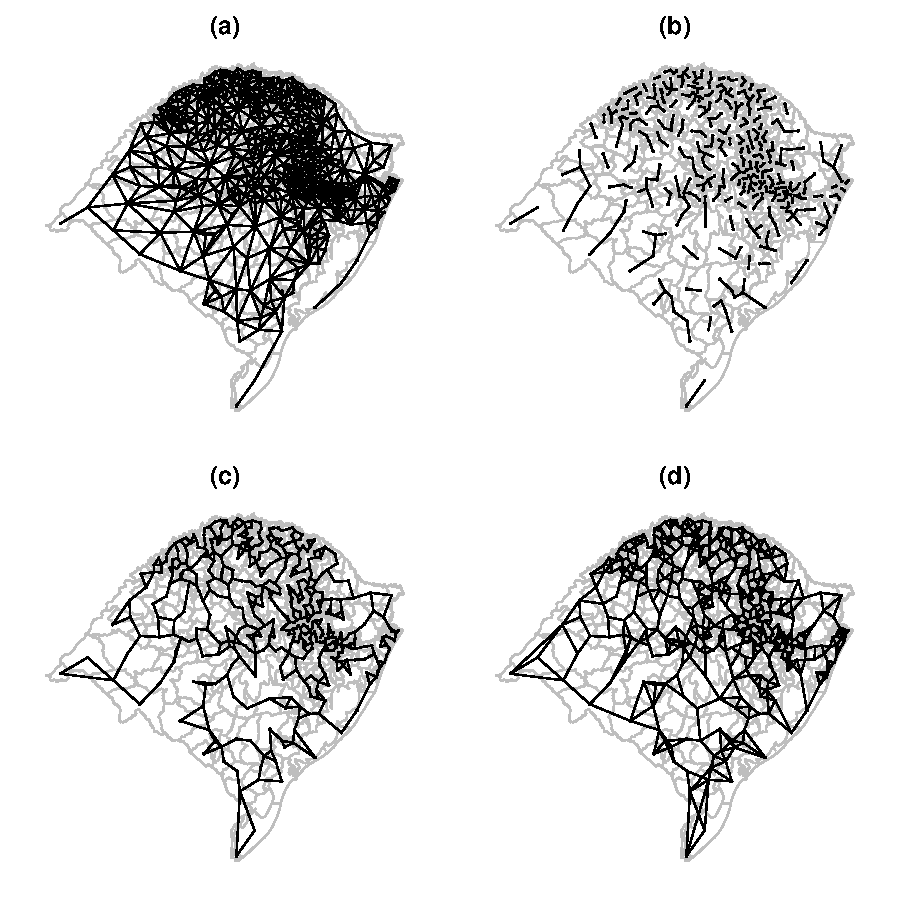
\includegraphics{TESE_DE_DOUTORADO_RENAN_FINAL-plot2}
\end{center}
\caption{Exemplo de Diferentes Especificações. (a) Vizinhos de contiguidade de 1ª ordem. (b) k-NN de 1ª ordem. (c) k-NN de 2ª ordem. (d) k-NN de 3ª ordem.}
\label{fig:especif}
\end{figure}

Para informações sobre estruturas de matrizes de vizinhança em econometria espacial, recomenda-se o Capítulo 9 de \co{bivand2008spatialwithR}.

\subsection{Índices de Moran\label{subsec:IdeMoran_Indice}}

Assim como há a correlação linear de Pearson para variáveis aleatórias, \co{moran1950biometrika} introduziu o conceito de autocorrelação espacial em que, dada uma estrutura espacial estabelecida de uma variável aleatória $Y$, o índice $I$ de Moran pode ser dado por:
\begin{align}
I=\frac{1}{\sum_{i\neq j}w_{ij}}\sum_{i\neq j}w_{ij}\left ( \frac{y_i-\bar{y}}{s_y} \right )\left ( \frac{y_j-\bar{y}}{s_y} \right )
\end{align}
onde $w_{ij}$ é dado pela matriz de pesos apresentada na seção anterior. A especificação do $I$ de Moran faz com que seus valores possam variar de -1 a 1.

\subsection{Modelos Autoregressivos Condicionais\label{subsec:CAR_Indice}}

Os modelos autoregressivos condicionais (doravante referenciados como CAR, do inglês \textit{conditional autoregressive models}) é uma proposta de \co{besag1974} de uma estrutura condicional para os dados. Considerando \textit{n} áreas de uma variável aleatória $\boldsymbol{x}=(x_1,...x_n)$, cada uma caracterizada por um grupo de vizinhos $N_{(i)}$, assume-se que $x_i$ segue a seguinte distribuição:
\begin{align}
x_i|\boldsymbol{x}_{-i}\sim Normal\left ( \mu_i+\sum_{j=1}^{n}r_{ij}\left ( x_j-\mu_j \right ),s_{i}^{2} \right )
\end{align}
onde $\mu_j$ é a média da área $j$ e $s_{i}^{2} = \sigma_{x}^{2}/N_i$ é a variância da área $i$, que depende do número de vizinhos ($N_i=\#N_{(i)}$) o que faz com que à medida que o número de vizinhos da área $i$ aumente, sua variância diminua. Esta estrutura de variância estabelece que na presença de alta correlação espacial, quanto mais vizinhos uma área tiver, mais informação teremos para estimar o seu efeito aleatório, enquanto que o parâmetro de variância $\sigma_{x}^{2}$ controla a variação dos efeitos aleatórios estruturados espacialmente. A quantidade $r_{ij}$ indica a proximidade espacial e é calculada como $\phi \times W_{ij}$, onde $W_{ij}=a_{ij}/N_{i}$, $a_{ij}$ é 1 se as áreas $i$ e $j$ são vizinhas e 0 caso contrário, enquanto que o parâmetro $\phi$ controla a adequação da distribuição.

Nos modelos aqui analisados, a distribuição da ocorência de crimes possui a seguinte verossimilhança:
\begin{align}
y_i|\lambda_i\sim Poisson(\lambda_i)
\end{align}
onde a média $\lambda_i$ é definida em termos da taxa de risco $\rho_i$ e o número esperado de ocorrências $E_i$ onde $\lambda_i=\rho_i\times E_i$. Neste caso, o preditor linear adquire a seguinte forma:
\begin{align}
\eta_i = \log (\rho_i)=\alpha + u_i
\end{align}
onde o efeito aleatório $u_i$ segue uma especificação estruturada CAR descrita anteriormente. Um modelo alternativo também foi proposto por \co{besag1991} onde um termo não estruturado é incluído no preditor linear da seguinte forma:
\begin{align}
\eta_i = \log (\rho_i)=\alpha + u_i + \varepsilon_i
\end{align}
onde o efeito aleatório $u_i$ também segue uma especificação estruturada CAR, descrita anteriormente, e o termo $\varepsilon_i$ segue um termo não estruturado $\varepsilon_i \sim Normal\left ( 0,\sigma_{\varepsilon}^{2} \right )$. Este modelo é denominado CAR \textit{intrínseco} ou BYM, de \textit{Besag-York-Mollie}.

\subsection{Integrated Nested Laplace Approximation\label{subsec:INLA_Indice}}

A classe de modelos que a metodologia INLA trabalha é denominada modelos Gaussianos Latentes onde a variável dependente $y_i$ é assumida pertencer a uma família de distribuições onde a sua média $\mu_i$ é conectada a um preditor linear aditivo $\eta_i$ através de uma função de ligação $g(\mu_i)=\eta_i$ tal que
$$
\eta_{i}=\alpha+\sum_{j=1}^{n_{f}}f^{(j)}(u_{ji})+\sum_{k=1}^{\eta_{\beta}}\beta_{k}z_{ki}
$$
onde $\left\{ f^{(j)}(\cdot)\right\}$'s são funções desconhecidas das covariáveis $\boldsymbol{u}$ e os $\left\{ \beta_{k}\right\}$'s representam o efeito linear das covariáveis $\boldsymbol{z}$. Observe que, nesta representação, as covariáveis $\boldsymbol{z}$ representam um caso particular das funções desconhecidas das covariáveis $\boldsymbol{u}$. Neste modelo, todas as variáveis latentes, isto é, $\alpha$, $\left\{ f^{(j)}(\cdot)\right\}$ e $\left\{ \beta_{k}\right\}$ são assumidas Gaussianas \textit{a priori}. Em modelos espaciais, a dependência pode ser modelada usando a covariável espacial $\boldsymbol{u}$ como sendo $f^{(j)}(u_{s})=f_{s}^{(j)}$, onde $\mathit{s}$ representa a locação espacial ou região. Para maiores informações e aplicações da metodologia, incluindo para dados de homicídios, ver \co{rue2009approximate}, \co{martino2009implementing}, \co{martins2012bayesian}, \co{ruiz2011direct}, \co{blangiardo2013epidemiology} e \co{cortes2014dissertacao}.

\subsection{Modelos\label{subsec:modelos_INLA}}

Os modelos que foram estimados a fim de avaliar uma maneira mais otimizada as frequências de ocorrências criminais seguem variações das abordagens descritas anteriormente. A ideia foi combinar modelos mais parcimoniosos (isto é, com menor número de parâmetros) com modelos mais sofisticados que englobam tanto termos estruturados, não-estruturados e efeitos aleatórios temporais. Em suma, testamos quatro tipos de modelos: i) modelo somente com efeito aleatório estruturado de município (Eq. \ref{eq:besag}); ii) modelo com efeito aleatório estruturado de município mais efeito aleatório não-estruturado (Eq. \ref{eq:bym}); iii) modelo com efeito aleatório estruturado de município com componente temporal do tipo passeio aleatório (\textit{random walk}) de primeira ordem (Eq. \ref{eq:besag_rw1}); e, o modelo mais complexo, iv) modelo com efeito aleatório estruturado de município mais efeito aleatório não-estruturado com componente temporal do tipo passeio aleatório (\textit{random walk}) de primeira ordem (Eq. \ref{eq:bym_rw1}).

Todas as abordagens foram estimadas para todos os tipos de estruturas de vizinhança fazendo da abordagem INLA.

Modelo Besag/CAR:
\begin{align}
\label{eq:besag}
\begin{split} % Este ambiente é para poder ter um único número em todo o modelo
y_i|\lambda_i & \sim Poisson(\lambda_i)\\
\lambda_i & =\rho_i\times E_i\\
\eta_i & =\log (\rho_i)=\alpha + u_i\\
u_i & \sim Besag\
\end{split}
\end{align}

Modelo BYM:
\begin{align}
\label{eq:bym}
\begin{split}
y_i|\lambda_i & \sim Poisson(\lambda_i)\\
\lambda_i & =\rho_i\times E_i\\
\eta_i & =\log (\rho_i)=\alpha + u_i + \varepsilon_{i}\\
u_i & \sim Besag\\
\varepsilon_{i} & \sim Normal(0,\tau)\
\end{split}
\end{align}

Modelo Besag/CAR com efeito temporal de primeira ordem (RW1):
\begin{align}
\label{eq:besag_rw1}
\begin{split}
y_i|\lambda_i & \sim Poisson(\lambda_i)\\
\lambda_i & =\rho_i\times E_i\\
\eta_i & =\log (\rho_i)=\alpha + \theta_t + u_i\\
\theta_t & =\theta_{t-1} + \epsilon_i\\
u_i & \sim Besag\\
\epsilon_i & \sim Normal(0,\tau)\
\end{split}
\end{align}

Modelo BYM com efeito temporal de primeira ordem (RW1):
\begin{align}
\label{eq:bym_rw1}
\begin{split}
y_i|\lambda_i & \sim Poisson(\lambda_i)\\
\lambda_i & =\rho_i\times E_i\\
\eta_i & =\log (\rho_i)=\alpha + \theta_t + u_i + \varepsilon_i\\
\theta_t & =\theta_{t-1} + \epsilon_i\\
u_i & \sim Besag\\
\varepsilon_i & \sim Normal(0,\tau)\\
\epsilon_i & \sim Normal(0,\tau)\
\end{split}
\end{align}

Em termos de distribuições das prioris, adotou-se uma postura conservadora, onde todas as precisões (que podem ser vistas como o inverso da variância), tanto dos termos estruturados (modelo Besag) quanto dos não-estruturados seguem uma distribuição \textit{Gama} com parâmetros 1 e 0,0005, ou seja, $1/\sigma ^{2}=\tau \sim Gama(1;0,0005)$\footnote{$X \sim Gama(\alpha;\beta) \Rightarrow E(X)=\alpha/\beta$.}. Por fim, com o intuito de comparar os modelos, duas medidas foram utilizadas.

A medida CPO (do inglês \textit{Conditional Predictive Ordinate}) \cite{spiegelhalter2002} permite avaliar o poder preditivo dos modelos estimados, similar aos métodos de validação cruzada \cite{kohavi1995}, somando os valores estimados para cada ponto amostral, retirando-o da estimação do modelo. A estatística de resumo fornecida pelo critério de CPO é o LPML\footnote{$\mbox{LPML}=-\sum_{i=1}^{n}\log\left\{ \pi\left(y_{i}\mid\boldsymbol{y}_{-i}\right)\right\}$} (do inglês, \textit{Logarithm of Pseudo Marginal Likelihood}), que avalia o poder preditivo do modelo e, na sua especificação, baixos valores de LPML indicam um bom poder preditivo.

As medidas DIC (do inglês \textit{Deviance Information Criteria}) \cite{gelfandBS1992,deyBio1997} são utilizadas na modelagem de inferência Bayesiana para avaliar a qualidade do modelo estimado penalizando pela quantidade do número de parâmetros, similar às medidas de AIC (do inglês \textit{Akaike Information Criteria}) \cite{akaike1973}. Elas fazem um ajuste balanceando o \textit{trade-off} entre o erro de ajuste e a sobreparametrização. Sendo assim, quanto menor o seu valor, melhor é a qualidade do ajuste destes modelos.


\section{Base de Dados e Penas Criminais\label{subsec:Base_Penas_Indice}}

A base de dados utilizada compila informações de ocorrências criminais disponibilizados pela Secretaria de Segurança Pública do Rio Grande do Sul\footnote{A base pode ser acessada no link http://www.ssp.rs.gov.br/ ou também na base de dados FEEDADOS da Fundação de Economia e Estatística através do link http://feedados.fee.tche.br/} (SSP-RS), que possui vínculo com órgãos como a Brigada Militar, Polícia Civil, Superintendência de Serviços Penitenciários e Instituto Geral de Perícias. Segundo \co{monteiro2009mono}, em 2007 foram instituídos, pelo então secretário José Franscisco Mallmann, 13 indicadores que tinham como objetivo retratar a realidade criminal no estado. Estes indicadores incluem as seguintes classes criminais: homicídio doloso, furto, furto de veículo, roubo, latrocínio, roubo de veículo, extorsão, extorsão mediante sequestro, estelionato, delitos relacionados à corrupção, delitos relacionados a armas e munições, posse de entorpecentes e tráfico de entorpecentes. Todas as ocorrências abrangem todos os 496 municípios do estado\footnote{O município de Pinto Bandeira foi excluído deste trabalho, uma vez que sua criação foi somente a partir do ano de 2013.} e os dados são anuais, iniciados em 2002. Neste estudo, no entanto, somente alguns crimes foram utilizados para a criação do índice geral de criminalidade, pois o objetivo é usar um conjunto de delitos que afetam diretamente o cotidiano do bem-estar social no que tange à relação direta entre a perda de um bem ou a vivência de um trauma devido ao contato direto interpessoal com o agressor resultando somente no uso do homicídio doloso (HomDol), roubo (Roub), roubo de veículos (RoubVei), latrocínio (Latro), furto (Furt), furto de veículos (FurtVei) e extorsão mediante sequestro (ExtoMS).

Com relação às ponderações criminais, optou-se por seguir \co{freitas2016xixeeg}, que fizeram uso da previsão da pena em termos de período de reclusão de acordo com o Código Penal Brasileiro, conforme a Tabela \ref{tab:penas}. Vale destacar que o código penal é bem específico em termos penais para diferentes tipos de crime. Por exemplo, no caso do furto\footnote{Artigo 155 - Subtrair, para si ou para outrem, coisa alheia móvel} (reclusão, de um a quatro anos), é possível classificá-lo como qualificado (reclusão de dois a oito anos) ou de coisa comum (detenção, de seis meses a dois anos). No entanto como não é possível saber qual a subcategoria do furto na base de dados da SSP-RS, optou-se por adotar a pena do grupo de maior nível hierárquico.

\begin{table}[H]
\caption{Penas dos crimes considerados no índice}
\label{tab:penas}
\centering
\begin{tabular}{lr}
  \hline
Crime & Penas \\ 
  \hline
Homicídio Doloso & 6 a 20 \\ 
Furto & 1 a 4 \\ 
Furto de Veículo & 1 a 4 \\ 
Roubos & 4 a 10 \\ 
Latrocínio\tablefootnote{Roubo seguido de morte.} & 20 a 30 \\ 
Roubo de Veículo & 4 a 10 \\ 
Extorsão mediante sequestro & 8 a 15 \\ 
   \hline
\tiny{Fonte: Elaboração própria.}
\end{tabular}
\end{table}




\section{Agregação do Índice\label{subsec:agregacao_Indice}}

De posse das estimativas geradas das ocorrências, apresenta-se o indicador geral de criminalidade combinando as estimativas. Conforme foi mostrado na Seção \ref{subsec:Base_Penas_Indice}, vamos ponderá-lo de acordo com a sua menor pena\footnote{Acredita-se que grande parte dos criminosos condenados não cumprem toda a pena sentenciada e, portanto, optou-se escolher pela menor pena prevista. Ademais, a escolha de outro valor entre o intervalo penal poderia ampliar a magnitude destes pesos devido a heterogeneidade de amplitudes entre os diferentes crimes.} prevista em no Código Penal. Sendo assim, o índice da região \textit{i} tem um formato simples conforme a Equação \ref{eq:icrime_RS}:
\begin{equation}
\label{eq:icrime_RS}
ICrimeRS_i=\frac{\sum_{j=1}^{k}y_{ij}\times w_j}{População_i} \times 365
\end{equation}
onde a variável \textit{j} é o indexador de tipo de crime (que varia de 1 até \textit{k}), \textit{y} é a quantidade de ocorrência criminal e \textit{w} é o pena mínima prevista em lei de acordo com a Tabela \ref{tab:penas}.

O ICrimeRS possui uma interpretação prática em termos de mensuração global da criminalidade. A soma do numerador representa a soma da pena mínima que o agressor de cada ocorrência deveria cumprir, em tese, de uma determinada região \textit{i}. Por exemplo, supondo que o índice é composto apenas por latrocínio e homicídio e num determinado ano houve 2 latrocínios e 10 homicídios. Este numerador resultaria em $2\times 20 + 10\times 6 = 100$ anos de reclusão se todos fossem condenados pela pena mínima. Para padronização do número, divide-se por toda a população e multiplica-se por 365 para dar o resultado em dias para melhorar a interpretabilidade. Exemplificando para um município, o indicador pode responder a seguinte pergunta: \textit{"Supondo que todos os crimes sejam julgados e condenados pela pena mínima, em Porto Alegre, quantos dias do ano cada habitante porto-alegrense teria que passar na cadeia para pagar por todos os crimes cometidos?"}. Ou seja, se o ICrimeRS de Porto Alegre for 50 para um determinado ano, isso significado que, em média, \textbf{todos} os habitantes teriam que passar 50 dias presos para pagar pelos crimes cometidos em um cenário em que houvesse todas condenações mínimas\footnote{A fim de ilustrar em termos rentáveis. Em 2014, segundo a Fundação de Economia  Estatística, o PIB per capita de Porto Alegre chegou a R\$43.457,67. Portanto, sob algumas hipóteses, a perda de PIB per capita, caso cada porto-alegrense passasse 50 dias encarcerado, seria de R\$5.953,11.}.

Vale ressaltar que a presente proposta de indicador possui limitações. Evidentemente que a hipótese de todos os crimes serem julgados e condenados é muito forte. Sabe-se que, por exemplo, grande parte dos homicídios cometidos não são resolvidos ou demoram consideravelmente até o seu julgamento. Adicionalmente, uma característica importante, que não está sendo levada em consideração, é a possibilidade de reincidência da mesma pessoa em determinado crime. Por exemplo, é possível que uma mesma pessoa (ou grupos de pessoas) seja responsável por mais de uma ocorrência de roubo num ano em uma região (ou várias regiões). No entanto, mesmo com estas ressalvas, a interpretabilidade e a relevância do indicador ainda é mantida, uma vez que ele não mede eficiência policial ou jurídica, mas sim a realização do fato criminal de uma determinada região e ano.







\section{Estatísticas Descritivas\label{sec:Resultados_Descritivos}}

A Figura \ref{fig:homDolRS} apresenta a evolução da taxa por 100.000 habitantes do homicídio doloso no estado do Rio Grande do Sul. Primeiramente, ressalta-se que o patamar em que esta série se encontra já é elevado uma vez que o seu valor mínimo, obtido no ano de 2004, é de 12,39 o que representa um número maior que o máximo considerado aceitável pela Organização das Nações Unidas (ONU), que classifica como violência epidêmica quando há mais de 10 mortes violentas para cada 100.000 habitantes\footnote{http://noticias.uol.com.br/cotidiano/ultimas-noticias/2013/11/05/todos-os-estados-do-pais-tem-assassinatos-em-niveis-epidemicos-aponta-estudo.htm}. Nesta figura podemos verificar a preocupante tendência crescente destas taxas principalmente a partir do ano de 2012 e alcançando o valor de 21,6 em 2015.

\begin{figure}
\begin{center}
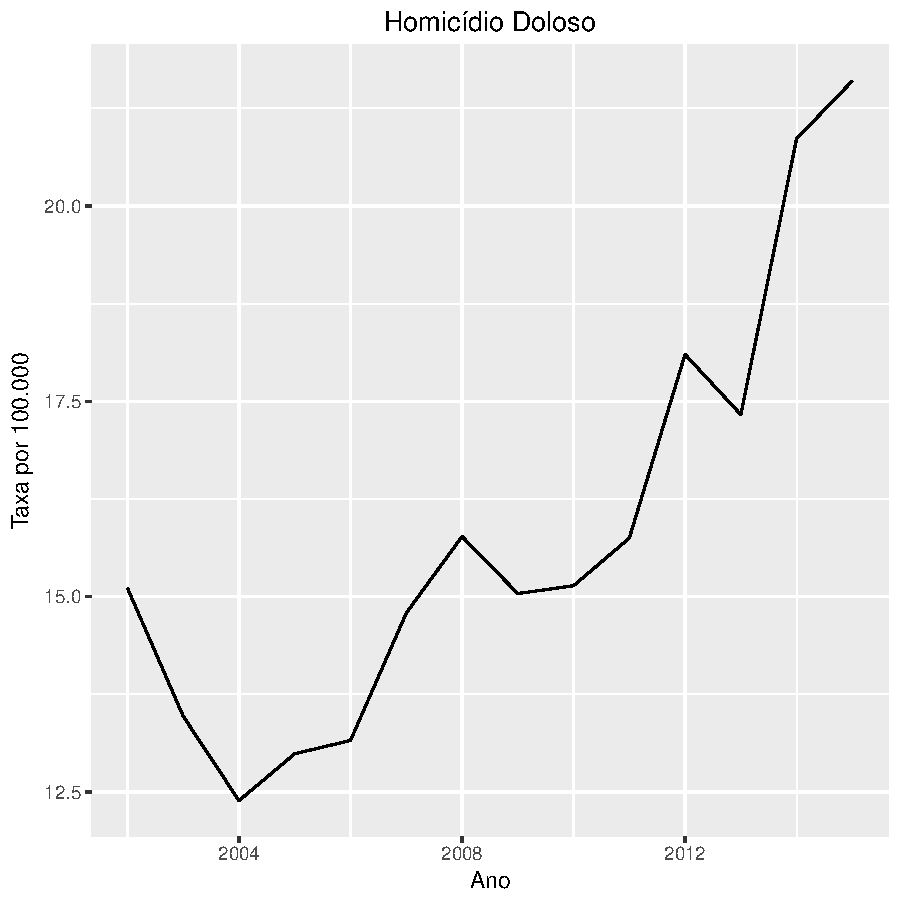
\includegraphics{TESE_DE_DOUTORADO_RENAN_FINAL-plot3}
\end{center}
\caption{Evolução do Homicídio Doloso no Rio Grande do Sul}
\source{Fonte: SSP-RS e FEE.}
\label{fig:homDolRS}
\end{figure}

Para os demais crimes do estado, a Figura \ref{fig:outroscrimesRS} apresenta a dinâmica evolutiva separadamente. Pelas magnitudes das taxas, é possível observar que o tipo de crime que tem o maior número de registros é o Furto que alcançou uma marca de 2431,6 casos por 100.000 habitantes no ano de 2003, mas posteriormente, esta série apresenta uma acentuada queda ao longo dos anos. O Roubo é o segundo crime com maior patamar, oscilando entre os valores de 405,81 em 2011 e o alto valor de 703,35 em 2015. É interessante analisar a dinâmica que o roubo apresentou no RS, em formato de \textit{U}, tendo seu início logo após o ano de 2007, mas alcançando valores consideráveis ao seu final. Esta característica em formato de \textit{U} também é observada nos crimes de Roubo de Veículos, Latrocínio e Furto de Veículos, sendo todos eles tendo início em períodos similares perto de 2006 e ascensões após o ano de 2010. Esta característica vai contra a impressão de que em geral as pessoas têm de que a criminalidade "está sempre aumentando". Os dados estaduais não apontam nesta direção, indicando algum acontecimento nestes períodos indicados. Por fim, mas não menos importante, observa-se a evolução errática da quantidade de extorsões mediante sequestro. Este tipo de crime se apresenta com menor grau de ocorrência criminal tendo taxas, em sua maior parte, menores que 0,3 casos por 100.000 habitantes. Para se ter noção da magnitude e da esparsidade de matriz de dados deste tipo de crime, em 2015 houve 18 registros e em 2014 (o maior valor da série histórica) registrou-se 37 casos em todo o estado. 

\begin{figure}
\begin{center}
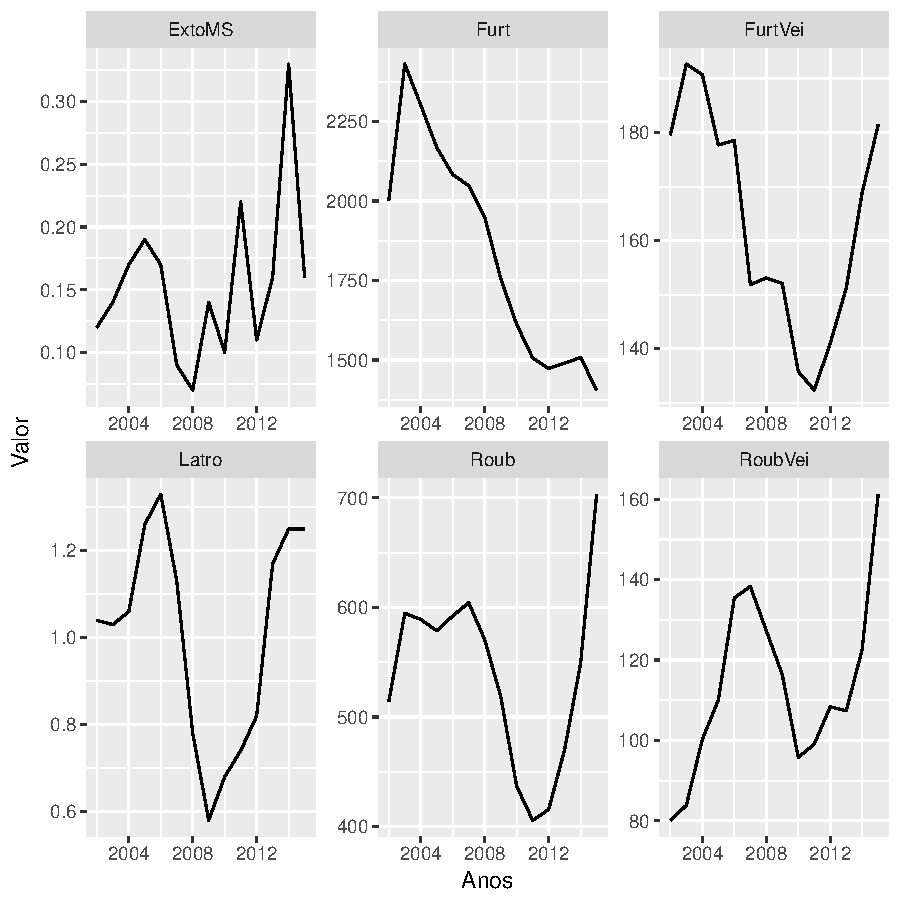
\includegraphics{TESE_DE_DOUTORADO_RENAN_FINAL-plot4}
\end{center}
\caption{Evolução de crimes selecionados no Rio Grande do Sul, 2002-2015}
\source{Fonte: SSP-RS e FEE.}
\label{fig:outroscrimesRS}
\end{figure}

As Figuras \ref{fig:hom_dol5} e \ref{fig:evol_crimes5} mostram a evolução dos crimes separados pelas cinco maiores cidades do RS, a saber, Porto Alegre, Caxias do Sul, Canoas, Pelotas e Santa Maria, respectivamente. A dinâmica evolutiva dos crimes é muito similar a apresentada no estado, tendo em vista que grande parte dos crimes acontecem nestas cidades. Somente na capital, Porto Alegre, para o ano de 2015, as ocorrências de homicídios representaram 24\% de todo o estado. Para os demais crimes e representação também foi acentuada\footnote{Porto Alegre representou 39\% de roubos, 52\% de roubo de veículos, 26\% de latrocínios, 20\% de furtos, 21\% de furto de veículos e 11\% de extorsões mediante sequestro.}.

É importante notar que as dinâmicas da Figura \ref{fig:evol_crimes5} são similares a do estado, onde todos os maiores municípios apresentaram queda em \textit{U} nos crimes de Roubo, Roubo de Veículos e Latrocínio e queda nos furtos. Por outro lado, o formato em \textit{U} dos furtos de veículos não é ilustrado quando mostrados somente estes municípios, pois ele foi causado basicamente pelos municípios de Porto Alegre, Canoas, São Leopoldo (3,9\% dos casos no estado em 2015), Santa Cruz do Sul (3,2\% dos casos no estado em 2015) e Passo Fundo (3,1\% dos casos no estado em 2015).

Algumas das principais hipóteses acerca desta característica do formato em \textit{U} de diversos municípios e no RS são discutidas em \co{kerber2016}. A principal é a de que esta característica tem estreita relação com a implementação do Programa Nacional de Segurança Pública com Cidadania (PRONASCI) no RS, em especial, na Região Metropolitana de Porto Alegre\footnote{Também discutida em \co{cidade2012implementaccao}.}. Além disto, neste período, diversas operações atreladas à repressão qualificada foram feitas. Na RMPA, em 2009, aconteceu a Operação Cova Rasa que fez diversas prisões estratégicas. Outros pontos discutidos foram as criações dos territórios de paz, os projetos sociais, Mulheres da Paz e Justiça Comunitária, construídos e financiados pela SENASP/Ministério da Justiça em muitos municípios. Outro fator que é levantado é o de que neste período foi realizada a estruturação dos Gabinetes de Gestão Integrada Municipal (GGIM) e das áreas com videomonitoramento e de audiomonitoramento. 

Além disso, foi criado o Índice de Municipalização da Segurança Pública (IMUSP). Notou-se que Canoas e Esteio foram os municípios com maior IMUSP. Argumenta-se que quanto maior o IMUSP, maior a redução de crimes patrimoniais, roubos e furtos em geral, atrelados à sensação de segurança\footnote{Apesar do medo estar relacionado com vitimização.}. \co{kerber2016} dizem que a gestão da informação e a integração das polícias com as Guardas Municipais foram decisivos no período de 2010 a 2012 e notaram que os municípios com mais ações do PRONASCI foram os que mais reduziram crimes, exceto os crimes letais, como homicídios. Por fim, os autores fazem a ressalva de que a dinâmica da produção das violências é multicausal e multifatorial. Ou seja, existem outros fatores que influenciaram, como a criação de secretarias de segurança municipais, a centralidade da agenda pública e política e a conjuntura econômica e política.

\begin{figure}
\begin{center}
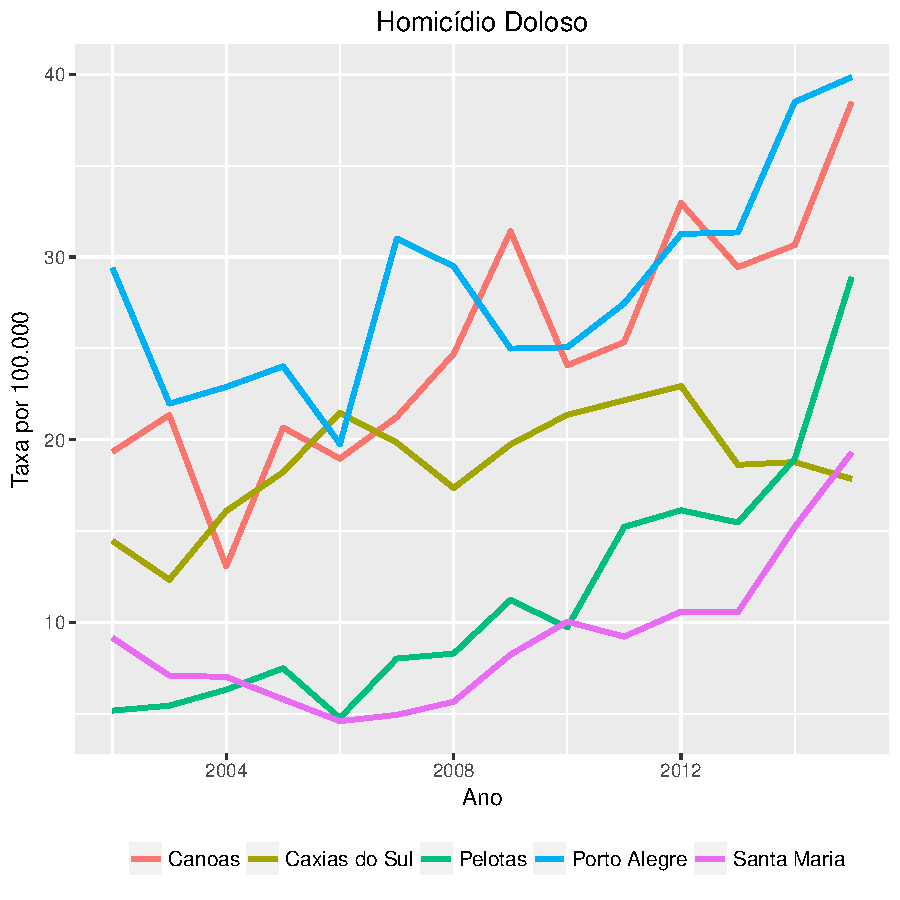
\includegraphics{TESE_DE_DOUTORADO_RENAN_FINAL-plot5}
\end{center}
\caption{Evolução de homicídios nos cinco maiores municípios}
\source{Fonte: SSP-RS e FEE.}
\label{fig:hom_dol5}
\end{figure}

\begin{figure}
\begin{center}
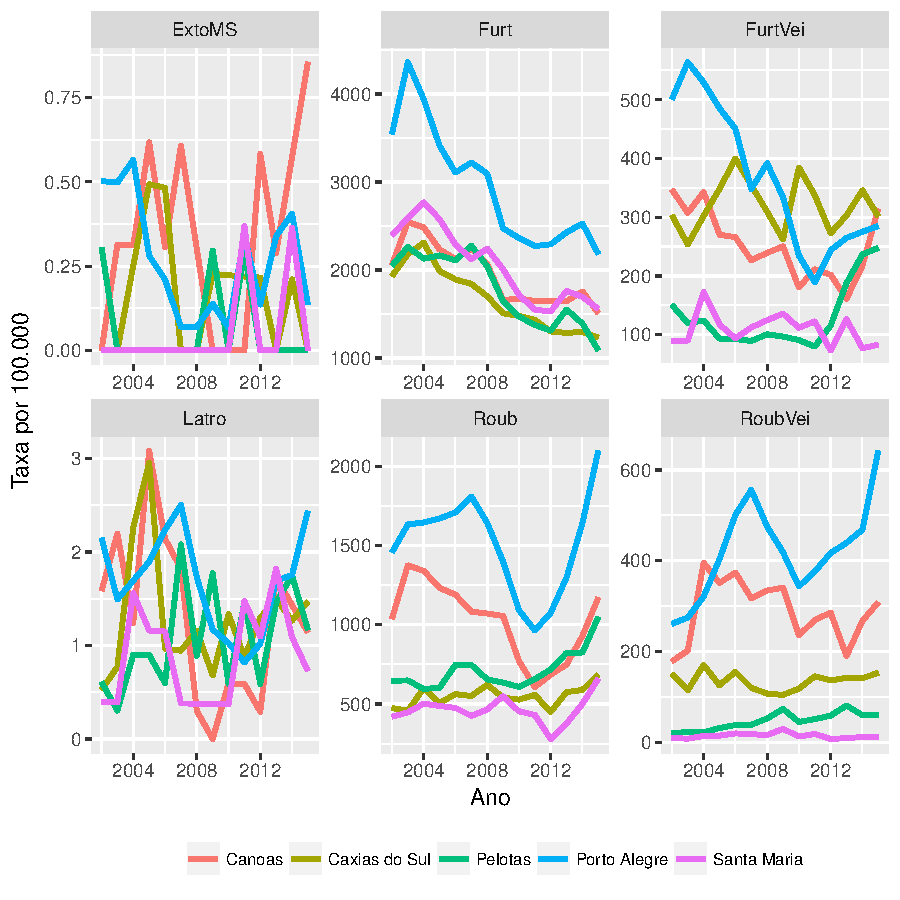
\includegraphics{TESE_DE_DOUTORADO_RENAN_FINAL-plot6}
\end{center}
\caption{Evolução de crimes selecionados nos cinco maiores municípios}
\source{Fonte: SSP-RS e FEE.}
\label{fig:evol_crimes5}
\end{figure}

\begin{table}[H]
\caption{Estatísticas Descritivas de crimes selecionados, 2015}
\label{tab:descritivas_2015}
\centering
\begin{tabular}{lrrrrrr} % Alinhamento esq, dir, dir...
  \hline
Crime & Min. & 1º Q. & Mediana & Média & 3º Q. & Máx \\ 
  \hline
Roub & 0.00 & 31.10 & 73.71 & 137.52 & 157.10 & 2097.96 \\ 
RoubVei & 0.00 & 0.00 & 0.00 & 26.35 & 30.26 & 642.40 \\ 
Latro & 0.00 & 0.00 & 0.00 & 0.62 & 0.00 & 24.27 \\ 
Furt & 0.00 & 696.70 & 959.69 & 1077.87 & 1325.01 & 5689.20 \\ 
HomDol & 0.00 & 0.00 & 0.00 & 10.01 & 17.25 & 90.99 \\ 
FurtVei & 0.00 & 18.59 & 50.83 & 70.24 & 92.68 & 500.63 \\ 
ExtoMS & 0.00 & 0.00 & 0.00 & 0.04 & 0.00 & 9.18 \\ 
   \hline
\tiny Fonte: Elaboração própria.
\end{tabular}
\end{table}


\begin{table}[H]
\begin{tiny}
\caption{Ranking municipal de taxas criminais - 2015}
\label{tab:ranking_2015}
\centering
\begin{tabular}{llllll}
  \hline
Crime & 1º lugar & 2º lugar & 3º lugar & 4º lugar & 5º lugar \\ 
  \hline
Roub & Porto Alegre & Alvorada & Cachoeirinha & Esteio & Novo Hamburgo \\ 
RoubVei & Porto Alegre & Novo Hamburgo & Cachoeirinha & São Leopoldo & Canoas \\ 
Latro & Riozinho & Cerro Branco & Caiçara & Campinas do Sul & Maquiné \\ 
Furt & Xangri-lá & Arroio do Sal & Imbé & Balneário Pinhal & Cidreira \\ 
HomDol & Esmeralda & Entre Rios do Sul & Ponte Preta & Porto Vera Cruz & Campestre da Serra \\ 
FurtVei & Santa Cruz do Sul & Campo Bom & Novo Hamburgo & Tramandaí & Bento Gonçalves \\ 
ExtoMS & Terra de Areia & Parobé & Novo Hamburgo & Alvorada & Canoas \\ 
   \hline
\multicolumn{6}{l}{Fonte: Elaboração própria.}
\end{tabular}
\end{tiny}
\end{table}

As Tabelas \ref{tab:descritivas_2015} e \ref{tab:ranking_2015} apresentam, respectivamente, as principais estatísticas descritivas de cada um dos crimes e os cinco municípios que apresentam as maiores taxas em 2015. Estas tabelas refletem apenas um retrato transversal da estrutura criminal do estado do Rio Grande do Sul, pois seus valores e rankings podem variar substancialmente entre cada um dos anos. Uma das características que mais chamam a atenção na primera tabela é a quantidade expressiva de zeros de medidas de locação (em especial, primeiro quartil, mediana e terceiro quartil) de diversos crimes, o que reflete a grande esparsidade da matriz de dados onde diversos municípios simplesmente não registram ocorrências criminais destas classificações. Em termos de rankings municipais, por exemplo, Porto Alegre, Alvorada e Cachoeirinha ficaram com as três primeiras posições no ranking de roubos; Porto Alegre, Novo Hamburgo e Cachoeirinha no roubo de veículos; Riozinho, Cerro Branco e Caiçara no latrocínio e os demais rankings podem ser visualizados.

Chama a atenção o nome de municípios atípicos no topo destas listas como o município de Esmeralda, Entre Rios do Sul e Ponte Preta para homicídios dolosos, assim como os três mencionados anteriormente para o crime de latrocínio. O município de Esmeralda, que fica próximo à fronteira nordeste do estado, apresentou a grande taxa de homicídios de 90,99, sendo que neste ano este município teve somente três homicídios, mas com uma população de apenas 3.297\footnote{Esmeralda apresentou somente um homicídio em 2003, 2005, 2006, 2007 e 2009, obtendo um outlier de três casos em 2015.}. Já para o ano de 2013, o município líder em taxa de homicídios é o pequeno município do centro do estado, São José do Herval. Este município tinha uma população de 2.123 habitantes e apenas três casos, o que resultou em uma taxa de 141,31\footnote{São José do Herval apresentou somente um homicídio em 2002, 2005, 2007 e 2014, obtendo um outlier de três casos em 2013.}. Neste mesmo ano, São José do Inhacorá teve três casos, alcançando uma taxa de 135,14 homicídios por 100.000 habitantes\footnote{O único outro caso de homicídio foi em 2008.}. Para o crime de latrocínio a ocorrência de apenas um caso em Riozinho em 2015 (com população de 4.121) foi suficiente para colocá-lo no topo da lista alcançando uma taxa de 24,3\footnote{Este foi o único caso de latrocínio neste município em toda a série histórica}. O mesmo caso ocorre com o município de Muliterno, com 1.879 habitantes, que também apresentou somente um caso de latrocínio em toda a série, em 2014, representando uma taxa de 53,2 por 100.000 habitantes. 

Já para os crimes que acontecem com uma frequência maior como roubo e roubo de veículos, os municípios mais populosos ficam no topo do ranking das taxas. Alguns destaques que podem ser levados em consideração são o município de Tio Hugo (população de 2.855), que teve sete roubos de carros em 2015, resultando numa taxa de 245,18, e Ciríaco (4.813 habitantes), que teve 17 roubos em 2014 (taxa de 353,21). Em termos de furtos e furtos de veículos a principal característica a ser observada é a elevada presença de municípios litorâneos, que se observa também nos demais anos e não somente em 2015, como Xangri-lá, Arroio do Sal, Imbé, Cidreira, Tramandaí e Balneário Pinhal. 

\co{cortes2016tdfee} argumenta que "grande parte dos registros de ocorrência se dá quando o patrimônio suprimido possui valor significativo para a vítima". Além disso, argumenta que "Em geral, os furtos pequenos (como o de bolsas, celulares, relógios, etc.), que ocorrem em centros urbanos, não são registrados pelas vítimas, talvez por descrença no sistema judiciário em punir o infrator ou pela falta de disposição de se dirigir a uma delegacia por objetos de menor valor. No entanto, em cidades litorâneas (...) tanto as taxas de furto quanto as de furtos de veículos são relativamente maiores. Isso pode se relacionar ao fato de que, devido ao componente sazonal, grande parte das residências litorâneas fique vazia ao longo do ano, propiciando, conforme a Teoria das Janelas de Oportunidade, a subtração ilícita de bens, sem que haja relação interpessoal com a vítima.". Esta questão da sazonalidade e as evidências de subestimação do fluxo de pessoas no litoral do estado, o que superestima as taxas de furtos de municípios litorâneos, é discutido em \co{zuanazzi2016}.

Em termos espaciais, a Tabela \ref{tab:I_de_Moran} abaixo apresenta os resultados da estimativa do índice I de Moran de autocorrelação espacial para as diferentes especificações das matrizes de vizinhança para as taxas criminais. Observa-se que não há diferenças substanciais entre os anos selecionados, indicando que a estrutura espacial, independente do tempo, possui relativa estabilidade. Com relação aos Roubos, observa-se que a estrutura espacial possui alta e significativa autocorrelação espacial, principalmente quando leva-se em consideração um número menor de vizinhos através das especificações de diferentes k-NN, ou seja, em um grafo com um número maior de ligações, esta correlação perde um pouco a sua magnitude, indicando que a taxa de Roubos de determinada região é mais influenciada por um número reduzido (neste caso, até três) de vizinhos. Como era esperado, grande parte da concentração deste tipo de delito se localiza na região metropolitana de Porto Alegre com alguns destaques para os municípios de Pelotas, Rio Grande, Uruguaiana, Santa Maria, Caxias do Sul e Passo Fundo. 

O Roubo de Veículos é altamente concentrado na região metropolitana onde Porto Alegre representa aproximadamente 50\% das ocorrências em todos os anos. Tendo isto em vista, a alta correlação espacial significativa possui uma magnitude pouco menor do que a observada para os Roubos, que estão mais espalhados e mais concentrados em municípios ''chave'' do estado. Ressalta-se, a maior magnitude quando considerados somente dois ou três municípios mais próximos na estrutura espacial. O latrocínio, em termos de taxas, possui uma variabilidade maior em termos espaciais, tendo em vista as já referidas especificidades deste tipo de crime. Seu mapa mostram valores dispersos para cada um dos anos devido à raridade de seu evento e isto se reflete no baixo valor do índice I de Moran estimado para cada um dos anos, resultando um valores próximos a zero e não-significativos. 

O crime de Furto, o que tem o maior número de registros, é altamente concentrado em municípios litorâneos, mas também apresenta um maior grau de espalhamento entre todos os outros municípios do estado. Mesmo pelo fato da maior parte dos municípios terem Furtos, este tipo de crime ainda apresenta uma significativa autocorrelação espacial (principalmente levando em consideração apenas um município mais próximo, ou seja, $k-NN$ de 1ª ordem) indicando que municípios próximos entre si se influenciam. 

Os Homicídios possuem uma leve autocorrelação espacial positiva, porém significativa, para as diferentes especificações e anos das séries. Sua representação espacial é afetada pela presença de outliers em municípios pequenos que apresentam altas taxas. No entanto, mesmo com a presença destes outliers, o nível de espraiamento é grande, porém com um certo efeito espacial, o que é traduzido nos valores do índice I de Moran que são, em sua maior parte, acima de 0,1. O Furto de Veículos, por seu turno, também apresenta um grau de espraiamento elevado, porém com uma estrutura de dependência espacial mais forte, chegando a valores significativos acima de 0,46 para o ano de 2015, considerando um único vizinho mais próximo. Por fim, a Extorsão Mediante a Sequestro, devido ao seu altíssimo grau de raridade, resulta em valores de autocorrelação espacial praticamente nulos e não-significativos devido à esparsidade da matriz de dados. 

\begin{table}[H]
\begin{center}
\begin{small}
\caption{I de Moran calculado para diferentes crimes, para anos selecionados e diferentes especificações da matriz de vizinhança}
\label{tab:I_de_Moran}
\centering
\begin{tabular}{rllllllll}
  \hline
 & Crime & Matriz & 2002 & 2005 & 2008 & 2009 & 2012 & 2015 \\ 
  \hline
1 & Roub & Cont. (1ª) & 0.48* & 0.518* & 0.515* & 0.505* & 0.466* & 0.556* \\ 
  2 & Roub & k-NN (1ª) & 0.619* & 0.76* & 0.721* & 0.695* & 0.604* & 0.692* \\ 
  3 & Roub & k-NN (2ª) & 0.617* & 0.701* & 0.646* & 0.651* & 0.585* & 0.669* \\ 
  4 & Roub & k-NN (3ª) & 0.591* & 0.672* & 0.623* & 0.622* & 0.564* & 0.635* \\ 
  5 & RoubVei & Cont. (1ª) & 0.518* & 0.613* & 0.593* & 0.575* & 0.527* & 0.535* \\ 
  6 & RoubVei & k-NN (1ª) & 0.428* & 0.647* & 0.583* & 0.604* & 0.552* & 0.571* \\ 
  7 & RoubVei & k-NN (2ª) & 0.62* & 0.718* & 0.625* & 0.636* & 0.576* & 0.608* \\ 
  8 & RoubVei & k-NN (3ª) & 0.608* & 0.739* & 0.652* & 0.646* & 0.549* & 0.586* \\ 
  9 & Latro & Cont. (1ª) & 0.017 & 0.067* & -0.007 & -0.016 & -0.015 & 0.038 \\ 
  10 & Latro & k-NN (1ª) & 0.023 & -0.014 & -0.015 & -0.014 & -0.015 & -0.038 \\ 
  11 & Latro & k-NN (2ª) & 0.058 & 0.039 & 0.001 & -0.021 & -0.021 & -0.036 \\ 
  12 & Latro & k-NN (3ª) & 0.038 & 0.059* & -0.007 & -0.017 & -0.015 & 0.053* \\ 
  13 & Furt & Cont. (1ª) & 0.341* & 0.391* & 0.368* & 0.333* & 0.355* & 0.335* \\ 
  14 & Furt & k-NN (1ª) & 0.617* & 0.715* & 0.644* & 0.602* & 0.596* & 0.505* \\ 
  15 & Furt & k-NN (2ª) & 0.537* & 0.592* & 0.54* & 0.513* & 0.525* & 0.452* \\ 
  16 & Furt & k-NN (3ª) & 0.455* & 0.512* & 0.484* & 0.454* & 0.453* & 0.388* \\ 
  17 & HomDol & Cont. (1ª) & 0.103* & 0.119* & 0.185* & 0.059* & 0.088* & 0.126* \\ 
  18 & HomDol & k-NN (1ª) & 0.085 & 0.052 & 0.177* & 0.106* & 0.125* & 0.124* \\ 
  19 & HomDol & k-NN (2ª) & 0.084* & 0.096* & 0.225* & 0.091* & 0.137* & 0.13* \\ 
  20 & HomDol & k-NN (3ª) & 0.103* & 0.105* & 0.204* & 0.075* & 0.088* & 0.128* \\ 
  21 & FurtVei & Cont. (1ª) & 0.323* & 0.276* & 0.27* & 0.32* & 0.365* & 0.322* \\ 
  22 & FurtVei & k-NN (1ª) & 0.358* & 0.26* & 0.263* & 0.42* & 0.442* & 0.464* \\ 
  23 & FurtVei & k-NN (2ª) & 0.444* & 0.322* & 0.288* & 0.382* & 0.396* & 0.45* \\ 
  24 & FurtVei & k-NN (3ª) & 0.419* & 0.314* & 0.277* & 0.361* & 0.39* & 0.402* \\ 
  25 & ExtoMS & Cont. (1ª) & -0.002 & -0.002 & -0.01 & -0.006 & -0.008 & -0.001 \\ 
  26 & ExtoMS & k-NN (1ª) & -0.005 & -0.009 & -0.008 & -0.007 & -0.006 & -0.003 \\ 
  27 & ExtoMS & k-NN (2ª) & -0.004 & -0.007 & -0.007 & -0.011 & -0.006 & 0.002 \\ 
  28 & ExtoMS & k-NN (3ª) & -0.003 & -0.002 & -0.007 & -0.003 & -0.007 & 0 \\ 
   \hline
\multicolumn{9}{l}{Fonte: Elaboração própria.} \\
\multicolumn{9}{l}{Nota: O asterisco (*) representa significância a 5\%.}
\end{tabular}
\end{small}
\end{center}
\end{table}

Recentemente, uma ferramenta que possibilita a visualização dos dados de criminalidade do Rio Grande do Sul, a partir de séries temporais, gráficos de relação, mapas, assim como autocorrelações espaciais (para diferentes especificações da matriz de vizinhança), é o \textbf{CrimeVis} da Fundação de Economia e Estatística. Nesta ferramenta, é possível navegar e interagir dinamicamente entre as diferentes opções de visualização dos dados aqui apresentados. O CrimeVis pode ser acessado em http://visualiza.fee.tche.br/crime.

\section{Resultados\label{sec:modelos_indice}}

Os modelos estimados segundo a Seção \ref{subsec:modelos_INLA} foram comparados fazendo uso do DIC e do LPML. Os valores do LPML se encontram na Tabela \ref{tab:LPML}.

\begin{table}[H]
\begin{center}
\begin{tiny}
\caption{LPML para diferentes especificações e diferentes matrizes}
\label{tab:LPML}
\centering
\begin{tabular}{llrrrrrrr}
  \hline
Matriz & Especificação & Roubo & RouboVei & Latro & Furto & HomDol & FurtVei & ExtoMS \\ 
  \hline
Cont. (1ª) & Besag & 25419.99 & 11742.86 & 2075.90 & 52413.51 & 8021.24 & 22301.31 & 590.16 \\ 
Cont. (1ª) & BYM & 25419.01 & 11741.85 & 2075.66 & 52413.63 & 8020.62 & 22300.33 & 590.16 \\ 
Cont. (1ª) & Besag + RW1 & 25444.43 & 11805.33 & 2076.24 & 52368.41 & 8023.76 & 22237.35 & 590.21 \\ 
Cont. (1ª) & BYM + RW1 & 25442.21 & 11800.29 & 2076.03 & 52370.02 & 8023.52 & 22234.19 & 590.22 \\ 
k-NN (1ª) & Besag & 29184.34 & 17460.42 & 2147.53 & 52415.55 & 9527.48 & 24611.89 & 623.52 \\ 
k-NN (1ª) & BYM & 28735.78 & 16916.85 & 2134.61 & 52541.77 & 9338.64 & 24262.77 & 616.78 \\ 
k-NN (1ª) & Besag + RW1 & 29194.09 & 17558.20 & 2147.76 & 52370.63 & 9520.94 & 24517.45 & 623.59 \\ 
k-NN (1ª) & BYM + RW1 & 28744.92 & 16983.56 & 2134.44 & 52475.20 & 9336.73 & 24143.70 & 618.19 \\ 
k-NN (2ª) & Besag & 25425.73 & 12376.43 & 2155.34 & 52413.47 & 9601.24 & 22312.34 & 625.27 \\ 
k-NN (2ª) & BYM & 116942.77 & 58923.96 & 2170.16 & 88132.22 & 10244.07 & 49997.24 & 626.30 \\ 
k-NN (2ª) & Besag + RW1 & 25449.27 & 12437.28 & 2155.35 & 52370.74 & 9598.03 & 22368.72 & 625.27 \\ 
k-NN (2ª) & BYM + RW1 & 28318.18 & 33458.38 & 2170.29 & 56544.52 & 10263.77 & 33539.89 & 626.30 \\ 
k-NN (3ª) & Besag & 25423.06 & 12342.54 & 2157.44 & 52412.85 & 8726.26 & 22305.15 & 624.44 \\ 
k-NN (3ª) & BYM & 116979.91 & 58353.86 & 2172.73 & 90182.97 & 10329.64 & 49515.16 & 626.32 \\ 
k-NN (3ª) & Besag + RW1 & 25447.32 & 12412.15 & 2157.35 & 52368.22 & 8699.60 & 22241.59 & 624.59 \\ 
k-NN (3ª) & BYM + RW1 & 25565.82 & 33097.15 & 2172.89 & 56663.46 & 10369.80 & 33618.43 & 626.37 \\ 
   \hline
\multicolumn{9}{l}{Fonte: Elaboração própria.}
\end{tabular}
\end{tiny}
\end{center}
\end{table}


Os valores do DIC para os modelos estimados podem ser vistos na Tabela \ref{tab:DIC}.

\begin{table}[H]
\begin{center}
\begin{tiny}
\caption{DIC para diferentes especificações e diferentes matrizes}
\label{tab:DIC}
\centering
\begin{tabular}{llrrrrrrr}
  \hline
Matriz & Especificação & Roubo & RouboVei & Latro & Furto & HomDol & FurtVei & ExtoMS \\ 
  \hline
Cont. (1ª) & Besag & 49748.71 & 22952.88 & 4150.39 & 100654.70 & 15975.00 & 44451.91 & 1179.17 \\ 
Cont. (1ª) & BYM & 49746.27 & 22949.99 & 4149.81 & 100654.47 & 15973.04 & 44448.67 & 1179.15 \\ 
Cont. (1ª) & Besag + RW1 & 49690.41 & 22947.45 & 4151.02 & 100477.84 & 15977.64 & 44462.45 & 1179.24 \\ 
Cont. (1ª) & BYM + RW1 & 49688.18 & 22944.77 & 4150.55 & 100478.17 & 15977.30 & 44458.96 & 1179.24 \\ 
k-NN (1ª) & Besag & 57239.63 & 34319.00 & 4294.40 & 100663.69 & 19005.37 & 49155.42 & 1246.90 \\ 
k-NN (1ª) & BYM & 56362.48 & 33239.63 & 4269.43 & 100983.19 & 18632.38 & 48445.20 & 1233.44 \\ 
k-NN (1ª) & Besag + RW1 & 57165.47 & 34294.24 & 4294.73 & 100496.22 & 18990.73 & 49141.97 & 1247.01 \\ 
k-NN (1ª) & BYM + RW1 & 56295.99 & 33190.24 & 4269.00 & 100767.21 & 18627.23 & 48408.08 & 1236.17 \\ 
k-NN (2ª) & Besag & 49772.66 & 24302.50 & 4309.83 & 100657.15 & 19152.10 & 44485.44 & 1250.52 \\ 
k-NN (2ª) & BYM & 231142.70 & 116952.17 & 4339.80 & 171989.60 & 20455.88 & 99960.90 & 1252.56 \\ 
k-NN (2ª) & Besag + RW1 & 49714.19 & 24279.69 & 4309.76 & 100478.71 & 19144.05 & 44785.79 & 1250.50 \\ 
k-NN (2ª) & BYM + RW1 & 55449.86 & 65740.68 & 4340.06 & 108971.87 & 20493.95 & 67182.64 & 1252.56 \\ 
k-NN (3ª) & Besag & 49768.63 & 24236.07 & 4313.94 & 100656.60 & 17403.92 & 44472.25 & 1248.83 \\ 
k-NN (3ª) & BYM & 231313.12 & 115829.00 & 4345.05 & 175962.87 & 20625.67 & 99200.93 & 1252.61 \\ 
k-NN (3ª) & Besag + RW1 & 49710.14 & 24229.56 & 4313.71 & 100479.81 & 17349.44 & 44482.71 & 1249.10 \\ 
k-NN (3ª) & BYM + RW1 & 49996.59 & 65035.74 & 4345.36 & 109202.52 & 20705.62 & 67400.28 & 1252.72 \\ 
   \hline
\multicolumn{9}{l}{Fonte: Elaboração própria.}
\end{tabular}
\end{tiny}
\end{center}
\end{table}

Com base nestes resultados, nota-se que a maioria dos modelos apontados por ambos os critérios, são modelos que fazem uso da estrutura de vizinhança supondo matriz de contiguidade de 1ª ordem. Os critérios de LPML apontaram para o modelo BYM em praticamente todos os crimes, com exceção do Furto de Veículos que apontou para o modelo BYM+RW1. Uma peculiaridade deste critério foi a de que, para o Furto, ele apontou para o modelo Besag+RW1 supondo estrutura de vizinhança com 3 vizinhos mais próximos. Já com relação ao critério do DIC, os modelos apontados foram BYM+RW1, BYM+RW1, BYM, Besag+RW1, BYM, BYM e BYM para, respectivamente, os crimes de Roubo, Roubo de Veículos, Latrocínio, Furto, Homicídio Doloso, Furto de Veículos e Extorsão Mediante Sequestro.

Uma coisa que é importante chamar a atenção é a de que, para a extorsão mediante sequestro, e para os dois crimes contra a vida (homicídio doloso e latrocínio), os critérios apontaram para o mesmo modelo (BYM). Tendo em vista que o critério de construção do LPML é objetivamente a capacidade preditiva do modelo, ele foi utilizado como critério de desempate para os demais crimes. Sendo assim, as abordagens resultantes foram BYM (Roubo), BYM (Roubo de Veículos), BYM (Latrocínio), Besag+RW1 (Furto), BYM (Homicídio Doloso), BYM+RW1 (Furto de Veículos) e BYM (Extrosão Mediante Sequestro). Todos eles supondo vizinhos de contiguidade de 1ª ordem, com exceção do Furto.


A Figura \ref{fig:rela_INLA_Bruto} mostra a relação de ocorrência entre as estimativas do modelo e dos dados brutos. Apesar de existir um \textit{cluster} de pontos destacado nos cantos superiores direitos da maioria dos gráficos, representando os 14 anos de Porto Alegre, aparentemente existe uma relação direta entre o INLA e o número de ocorrências em cada um dos crimes. Uma característica que foi avaliada foi a de que as estimativas obtidas pelo método INLA sobresuavizaram as estimativas e, portanto, optou-se por utilizar dois terços de seu peso para os valores estimados e um terço para os verdadeiros valores como \textit{proxy} do número de ocorrências\footnote{O critério de definição do peso foi definido a fim mitigar o efeito de sobresuavização.}.
%mas isto demonstrou-se uma característica desejável uma vez que a alta volatilidade apresentada em municípios pequenos se dissolveu e se aproximou mais de uma média global. 
%e, portanto, optou-se por utilizar a média entre os valores estimados e verdadeiros como \textit{proxy} do número de ocorrência.


\begin{figure}
\begin{center}
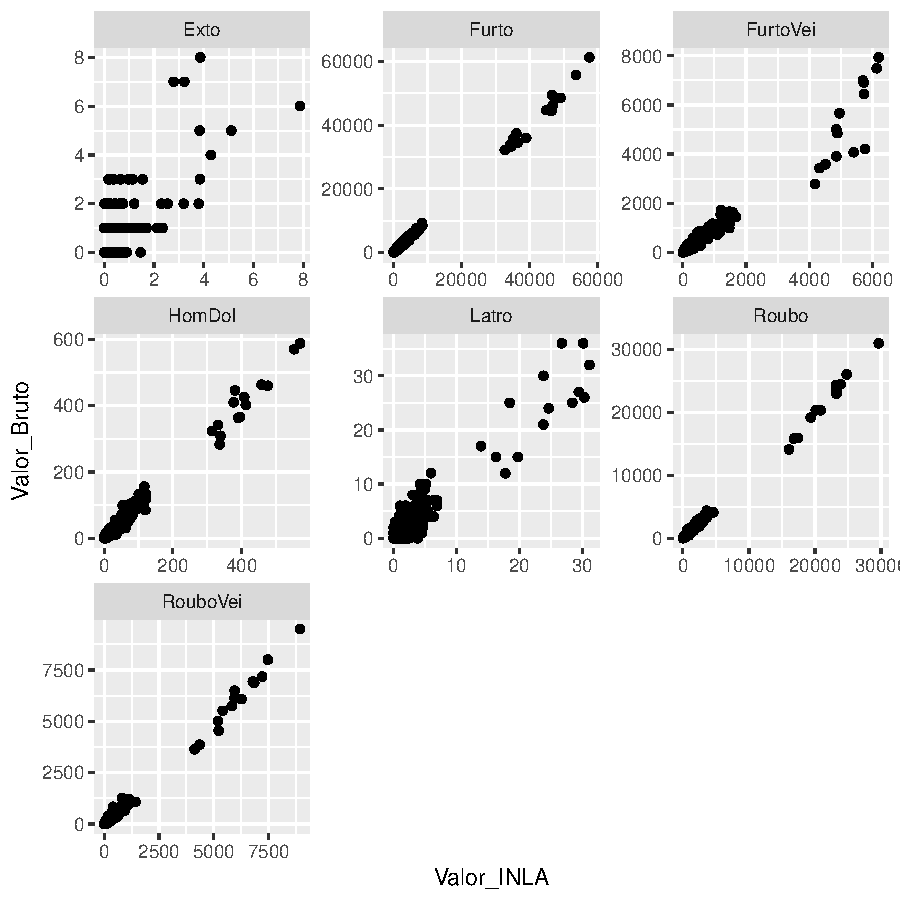
\includegraphics{TESE_DE_DOUTORADO_RENAN_FINAL-plot7}
\end{center}
\caption{Relação entre ocorrência estimada pelos modelos do INLA e ocorrência bruta (todos os anos e todos os municípios)}
%\captionsource{Relação entre ocorrência estimada pelos modelos do INLA e ocorrência bruta (todos os anos e todos os municípios)}{Elaboração própria.}
\source{Fonte: SSP-RS e elaboração própria.}
\label{fig:rela_INLA_Bruto}
\end{figure}


As Figuras \ref{fig:compara_homdol_muni_selecionados} e \ref{fig:compara_latro_muni_selecionados} ilustram o efeito do método utilizado na estimação do número de ocorrências esperado em cada região para homicídio e latrocínio. Nas duas figuras estão presentes um município representativo (Pelotas no primeiro e Alvorada no segundo) e três municípios mais problemáticos. É importante observar que a variância não é eliminada, mas existe uma suavização dos seus valores, bem como a presença de valores não-nulos quando o número de ocorrências é zero. Visualmente é possível ver que para o município de Esmeralda, por exemplo, o número de ocorrência é não-nulo para os anos próximos a 2012 e apresentaria menos de 2 casos de homicídio em 2015. Complementarmente, na Figura \ref{fig:compara_latro_muni_selecionados} o município de Riozinho apresenta valores não-nulos para toda a sua série histórica mostrando que, apesar de não ter tido nenhum latrocínio até 2015, existia uma probabilidade remota de acontecer pelo método usado.

\begin{figure}
\begin{center}
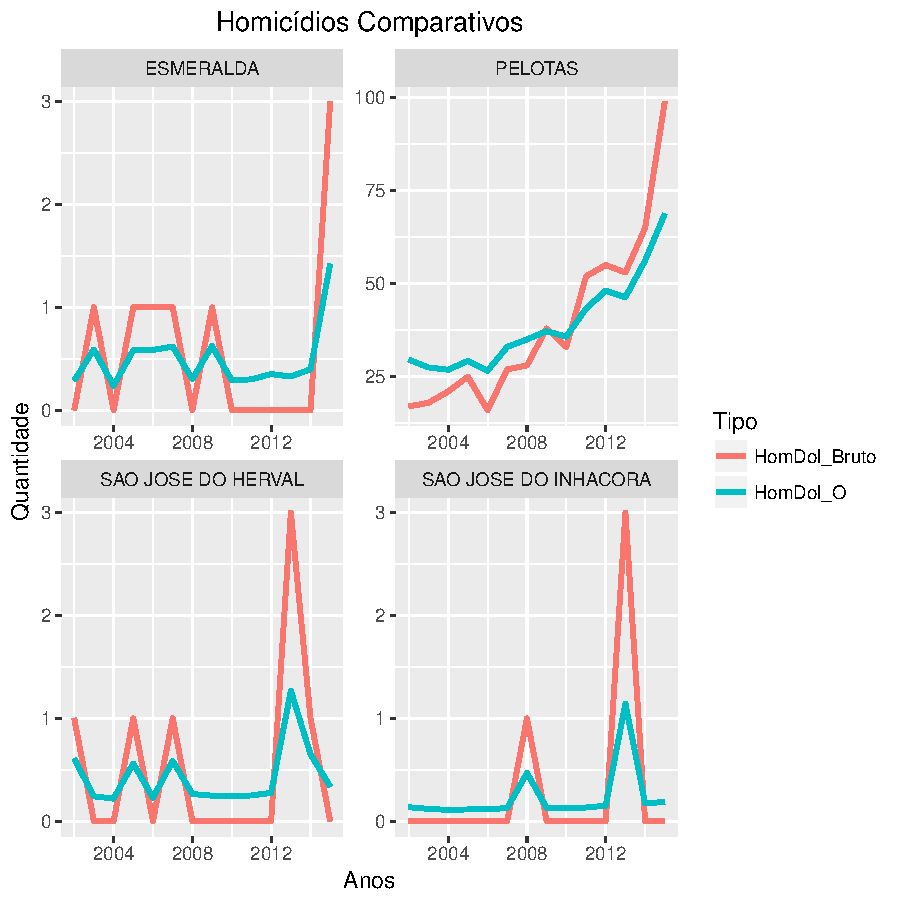
\includegraphics{TESE_DE_DOUTORADO_RENAN_FINAL-plot8}
\end{center}
\caption{Comparação de Número de Homicídios de municípios selecionados}
\source{Fonte: SSP-RS e elaboração própria.}
\label{fig:compara_homdol_muni_selecionados}
\end{figure}

\begin{figure}
\begin{center}
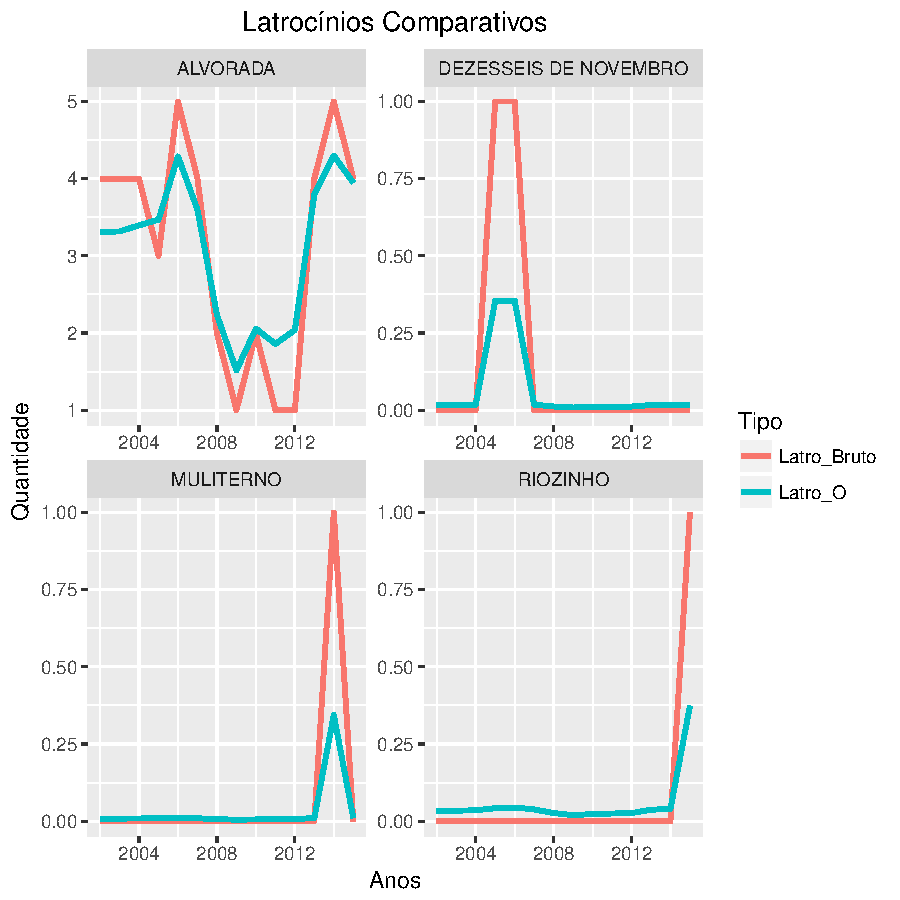
\includegraphics{TESE_DE_DOUTORADO_RENAN_FINAL-plot9}
\end{center}
\caption{Comparação de Latrocínios de municípios selecionados}
\source{Fonte: SSP-RS e elaboração própria.}
\label{fig:compara_latro_muni_selecionados}
\end{figure}

Uma das características desejadas do índice é, além de apresentar uma medida geral de criminalidade, poder segregar o indicador em dois tipos de crime: contra a vida e contra o patrimônio. Os crimes contra a vida compreendem os homicídios dolosos e os latrocínios, enquanto que os crimes contra o patrimônio referem-se aos cinco restantes. As Figuras \ref{fig:indices_top10} e \ref{fig:indices_low10} apresentam os principais resultados para dois conjuntos de municípios, onde, ambas as figuras, apresentam os resultados para o índice geral de criminalidade e os índices de crimes contra a vida e crimes contra o patrimônio.

A Figura \ref{fig:indices_top10} apresenta alguns dos principais municípios gaúchos evoluindo no tempo de acordo com cada um dos indicadores. A primeira característica a se notar no primeiro gráfico a esquerda é um padrão similar de comportamento caracterizado por um aumento nos anos iniciais, uma redução em meados de 2011 e 2012, seguido de um avanço subsequente. 

Porto Alegre é o município que apresenta o maior índice de criminalidade geral. Por exemplo, em 2015, o índice apresentou um valor de 49,15, o que significa que cada porto-alegrense deveria, em média, passar entre 49 e 50 dias dentro da cadeia neste ano para pagar por todos os crimes cometidos, supondo-se a condenação pela pena mínima prevista na lei brasileira. No entanto, ao analisar a desagregação de crimes contra o patrimônio e contra a vida, verificamos que quase 98\% deste indicador geral é composto por crimes contra o patrimônio uma vez que, apesar das suavizações obtidas pelo INLA, grande parte das ocorrências criminais são contra o patrimônio. O índice contra o patrimônio de 2015 resultou em 48,14 enquanto que contra a vida 1,01. Ainda analisando esta figura, é possível notar o acentuado grau de crimes contra a vida do município de Alvorada, onde em 2014 alcançou o patamar de 1,5.

Por outro lado, a Figura \ref{fig:indices_low10} mostra a dinâmica dos três índices para alguns municípios anômalos selecionados e comentados na Seção \ref{sec:Resultados_Descritivos}. Nestes gráficos é possível notar um comportamento mais errático em todas as séries temporais. O ICrime apresenta valores muito menores do que os dos municípios mais relevantes, tendo valores próximos a seis dias. Outra característica que chama a atenção é o fato de que novamente o índice é dominado pelas ocorrências criminais patrimoniais. Para o município de São José do Herval em 2006, por exemplo, é esperado que cada habitante passe 10,72 dias na cadeia para pagar por todos os crimes cometidos, sendo que desse tempo 10,46 seriam apenas referentes aos crimes patrimoniais. 

O gráfico mais à direita ilustra os índices dos crimes cometidos contra a vida. Nele notamos que, apesar do método ter suavizado as estimativas, uma vez que não existem valores nulos nas séries temporais e os saltos são mais amenos do que as informações brutas, existe uma razoável variabilidade nos valores. Em outras palavras, existem casos em que os índices de crimes contra a vida são bem grandes, principalmente quando comparados com os dez municípios mais relevantes do gráfico anterior. Neste gráfico, o município de Gramado dos Loureiros apresentou o valor valor de 1,92.

\begin{figure}
\begin{center}
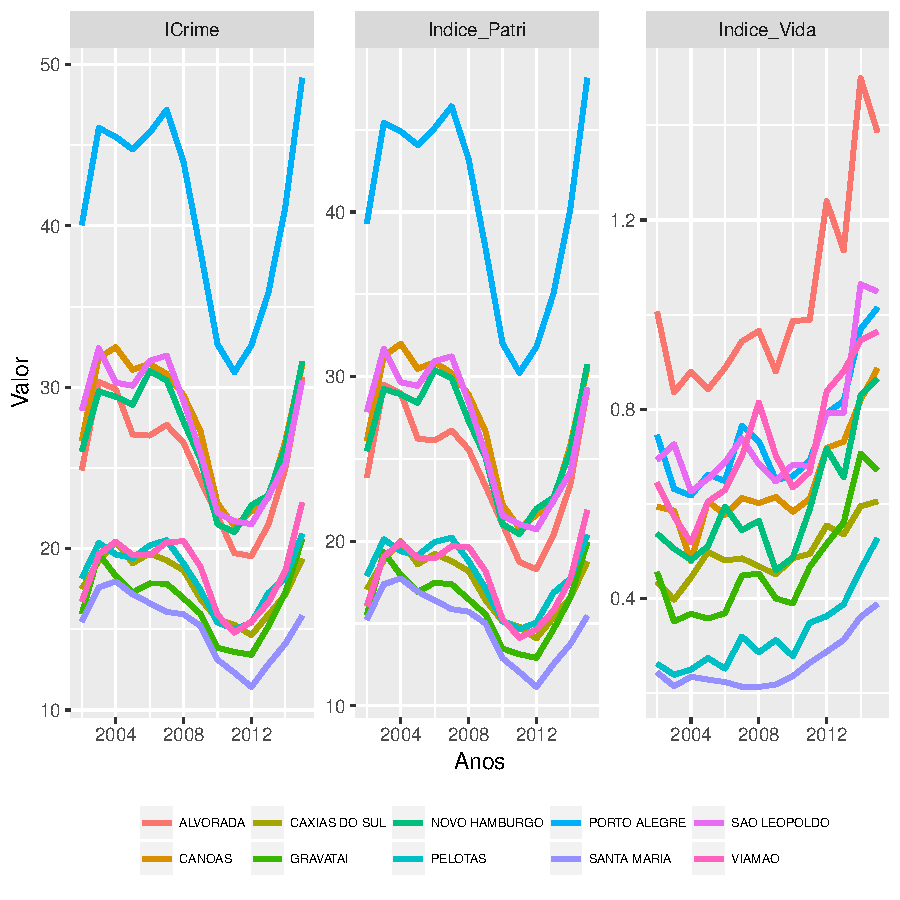
\includegraphics{TESE_DE_DOUTORADO_RENAN_FINAL-plot10}
\end{center}
\caption{Comparação dos índices para 10 municípios relevantes selecionados. O painel à esquerda mostra o ICrime geral, o painel central apresenta o índice contra o patrimônio e à direita o índice contra à vida.}
\source{Fonte: Elaboração própria.}
\label{fig:indices_top10}
\end{figure}

\begin{figure}
\begin{center}
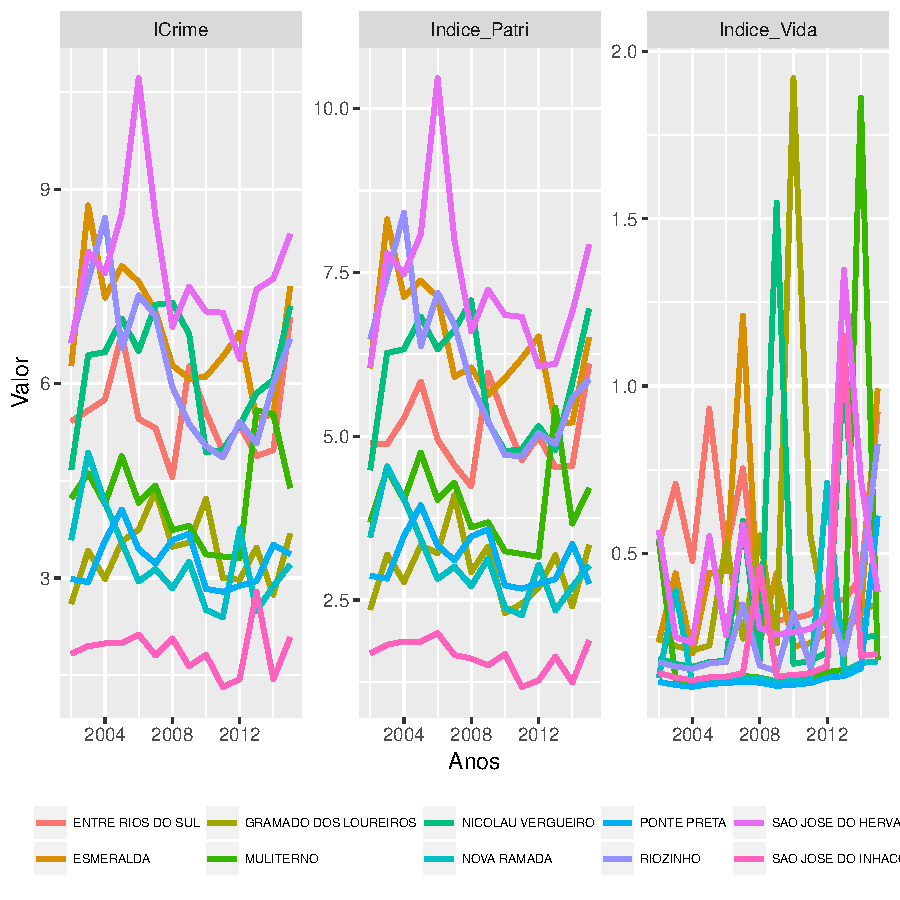
\includegraphics{TESE_DE_DOUTORADO_RENAN_FINAL-plot11}
\end{center}
\caption{Comparação dos índices para 10 municípios atípicos selecionados. O painel à esquerda mostra o ICrime geral, o painel central apresenta o índice contra o patrimônio e à direita o índice contra à vida.}
\source{Fonte: Elaboração própria.}
\label{fig:indices_low10}
\end{figure}


As Tabelas \ref{tab:rank_ICrime} e \ref{tab:rank_IVida} apresentam, para alguns anos recentes selecionados, municípios que tiveram os maiores e menores ICrime e Índice de Crime contra a Vida do Rio Grande do Sul. Nestas tabelas pode-se acompanhar os dez maiores municípios em cada ano, bem como os dez menores.

\begin{table}[H]
\caption{Rankings municipais do ICrime para anos selecionados: os 10 maiores e os 10 menores municípios}
\label{tab:rank_ICrime}
\begin{tiny}
\centering
\begin{tabular}{rllll}
  \hline
Posição & 2006 & 2009 & 2012 & 2015 \\ 
  \hline
1º & Xangri-La & Cidreira & Xangri-La & Porto Alegre \\ 
2º & Porto Alegre & Xangri-La & Porto Alegre & Xangri-La \\ 
3º & Cidreira & Porto Alegre & Cidreira & Cidreira \\ 
4º & Imbe & Imbe & Imbe & Imbe \\ 
5º & Balneario Pinhal & Arroio Do Sal & Tramandai & Novo Hamburgo \\ 
6º & Tramandai & Tramandai & Arroio Do Sal & Canoas \\ 
7º & Esteio & Balneario Pinhal & Esteio & Esteio \\ 
8º & Arroio Do Sal & Capao Da Canoa & Capao Da Canoa & Alvorada \\ 
9º & Sao Leopoldo & Canoas & Novo Hamburgo & Sao Leopoldo \\ 
10º & Canoas & Esteio & Balneario Pinhal & Tramandai \\ 
486º & Sao Joao Da Urtiga & Mariano Moro & Aurea & Ubiretama \\ 
487º & Novo Machado & Santa Maria Do Herval & Sao Joao Da Urtiga & Nova Candelaria \\ 
488º & Nova Boa Vista & Ubiretama & Candido Godoi & Santo Expedito Do Sul \\ 
489º & Candido Godoi & Sao Jose Do Inhacora & Sao Jose Do Inhacora & Canudos Do Vale \\ 
490º & Benjamin Constant Do Sul & Nova Candelaria & Mato Queimado & Sao Joao Da Urtiga \\ 
491º & Centenario & Candido Godoi & Nova Candelaria & Morrinhos Do Sul \\ 
492º & Nova Candelaria & Arroio Do Padre & Canudos Do Vale & Arroio Do Padre \\ 
493º & Novo Xingu & Mato Queimado & Travesseiro & Benjamin Constant Do Sul \\ 
494º & Arroio Do Padre & Morrinhos Do Sul & Arroio Do Padre & Novo Xingu \\ 
495º & Cruzaltense & Centenario & Centenario & Mato Queimado \\ 
496º & Mato Queimado & Cruzaltense & Morrinhos Do Sul & Centenario \\ 
   \hline
\multicolumn{5}{l}{Fonte: Elaboração própria.}
\end{tabular}
\end{tiny}
\end{table}




\begin{table}[H]
\caption{Rankings municipais do Índice Criminal contra a vida para anos selecionados: os 10 maiores e os 10 menores municípios}
\label{tab:rank_IVida}
\begin{tiny}
\centering
\begin{tabular}{rllll}
  \hline
Posição & 2006 & 2009 & 2012 & 2015 \\ 
  \hline
1º & Taquarucu Do Sul & Nicolau Vergueiro & Cotipora & Alvorada \\ 
2º & Pirapo & Novo Xingu & Vicente Dutra & Vicente Dutra \\ 
3º & Dezesseis De Novembro & Pouso Novo & Ivora & Balneario Pinhal \\ 
4º & Vicente Dutra & Pirapo & Alvorada & Sao Leopoldo \\ 
5º & Alvorada & Ciriaco & Viamao & Porto Alegre \\ 
6º & Itapuca & Dilermando De Aguiar & Alpestre & Esmeralda \\ 
7º & Vila Flores & Alvorada & Jaquirana & Viamao \\ 
8º & Dois Lajeados & Miraguai & Sao Leopoldo & Entre Rios Do Sul \\ 
9º & Cerro Grande Do Sul & Cerro Grande & Porto Alegre & Cidreira \\ 
10º & Andre Da Rocha & Capao Da Canoa & Capao Da Canoa & Canoas \\ 
486º & Boa Vista Do Burica & Augusto Pestana & Nova Candelaria & Nova Candelaria \\ 
487º & Westfalia & Salvador Do Sul & Augusto Pestana & Santo Cristo \\ 
488º & Tuparendi & Doutor Mauricio Cardoso & Salvador Do Sul & Sao Pedro Da Serra \\ 
489º & Ubiretama & Mariano Moro & Doutor Mauricio Cardoso & Antonio Prado \\ 
490º & Nova Candelaria & Centenario & Sao Pedro Da Serra & Doutor Mauricio Cardoso \\ 
491º & Mariano Moro & Sao Pedro Da Serra & Antonio Prado & Mariano Moro \\ 
492º & Centenario & Antonio Prado & Mariano Moro & Centenario \\ 
493º & Santo Cristo & Carlos Barbosa & Sananduva & Carlos Barbosa \\ 
494º & Doutor Mauricio Cardoso & Westfalia & Centenario & Westfalia \\ 
495º & Marcelino Ramos & Candido Godoi & Westfalia & Marcelino Ramos \\ 
496º & Candido Godoi & Marcelino Ramos & Candido Godoi & Candido Godoi \\ 
   \hline
\multicolumn{5}{l}{Fonte: Elaboração própria.}
\end{tabular}
\end{tiny}
\end{table}



A Tabela \ref{tab:rank_ICrime} mostra que, novamente, grande parte dos municípios que apresentam os maiores índices de criminalidade são municípios litorâneos. Em 2015, nota-se que estão presentes Xangri-lá, Cidreira, Imbé e Tramandaí nos dez maiores municípios, enquanto que Porto Alegre é o maior e Novo Hamburgo, Canoas, Esteio, Alvorada e São Leopoldo ocupam, respectivamente, da quinta à nona posição. Neste mesmo ano, municípios menos expressivos são os municípios mais ''seguros'' como Centenário, Mato Queimado e Novo Xingú. Em relação aos demais anos é possível notar um grau de robustez nas posições municipais. Por exemplo, a capital Porto Alegre está sempre entre as três cidades com maiores índices, Xangri-lá está sempre entre os dois maiores municípios, Imbé está na quarta posição em todos os anos, Esteio está sempre entre a sétima e décima posição, Centenário é um dos municípios com os menores índices estando sempre entre a 491ª e a última posição, Nova Candelária, Arroio do Padre e Mato Queimado são municípios com os menores índices em todos os anos selecionados.

Analisando a Tabela \ref{tab:rank_IVida}, que se referm aos rankings municipais de crimes contra a vida, vê-se que o comportamento dos rankings é mais errático entre os anos. Em 2015, Alvorada, Vicente Dutra, Balneário Pinhal, São Leopoldo e Porto Alegre lideram o ranking, enquanto Cândido Godoi, Marcelino Ramos, Westfalia, Carlos Barbosa e Centenário são as cidades com os menores índices de crime contra a vida. Em termos de comparabilidade inter-anual, é possível notar algumas características que se assemelham ao longo do tempo, mas com menor intensidade do que o ICrime. Por exemplo, o município de Alvorada se mostrou presente com altas taxas criminais vitais em todos os anos sempre ocupando altas posições nos rankings. A capital Porto Alegre e os municípios de São Leopoldo e Viamão se mostraram presentes em 2015 e 2012. Por outro lado, Cândido Godoi e Marcelino Ramos se mostraram sempre na última ou penúltima posição (exceto em 2012, Westfalia foi a penúltima), Mariano Moro é um município com baixas taxas criminais vitais, ocupando sempre entre a 489ª e 492ª posições e Westfalia e Doutor Maurício Cardoso estão presentes em todos os anos selecionados entre os municípios com menores taxas.

Comparando com a Tabela \ref{tab:ranking_2015}, apresentada na Seção \ref{sec:Resultados_Descritivos}, é imperativo que se note algumas semelhanças, mas sobretudo mudanças substanciais quando se olha o ano de 2015. Apesar de existir um grande indício de que o ICrime possui uma relação intrínseca com o tipo de crime de maior ocorrência (o Furto), que tipicamente apresentam as maiores taxas em municípios do litoral norte, foi Porto Alegre que liderou o ICrime em 2015 com um valor de 49,15. No entanto, o efeito do Furto no ICrime neste ano possui uma relevância, uma vez que Xangri-lá, Imbé, Cidreira são cidades que apresentam algumas das maiores taxas de Furto (Tabela \ref{sec:Resultados_Descritivos}) e maiores ICrime (Tabela \ref{tab:ranking_2015}). Com relação aos crimes contra a vida, as diferenças são substanciais, pois o município que lidera o ranking de mais perigoso em termos de crimes vitais é Alvorada, que não está presente nas cinco maiores taxas brutas de latrocínio ou de homicídio. Outra característica importante de se ressaltar é a de que o município de Esmeralda que apresentava a grande taxa de 91 homicídios por 100 mil habitantes, liderando o ranking, caiu para a sexta posição de crimes contra a vida. Adicionalmente, cidades que não apresentavam altas posições em termos de taxas brutas de homicídios e latrocínios, apareceram como altamente violentas, como é o caso de Porto Alegre, Vicente Dutra, Viamão e Canoas.

É interessante comparar também os resultados obtidos com o indicador sugerido por \co{freitas2016xixeeg}\footnote{Com relação a esta comparação, algumas ressalvas devem ser feitas. A parametrização do indicador de \co{freitas2016xixeeg} é em termos de bem-estar. Ou seja, é a taxa de crimes subtraído de um. Sendo assim, estamos comparando os municípios com maiores índices aqui apresentados com os menores índices do seu trabalho. Além disso, só foi realizado o índice para o ano de 2013, utilizando 14 tipos de crime, enquanto que no presente trabalho construímos o indicador para diversos anos e contemplamos sete tipos de crime.}. Analisando o ano de 2012 da Tabela \ref{tab:rank_ICrime}, nota-se um padrão de municípios litorâneos no topo da lista e municípios mais atípicos no final da lista. Este padrão não é similar ao resultado desses autores, pois a sua abordagem fez uma padronização prévia entre zero e um das taxas criminais, retirando o efeito da magnitude de cada crime, o que resulta em municípios metropolitanos com menor bem-estar. Ademais, nos municípios com menores índices de criminalidade do trabalho de \co{freitas2016xixeeg} não existe diferenciação de valor, onde os 29 municípios mais ''seguros'' apresentam o mesmo valor de índice até a terceira casa decimal. Sendo assim, as diferentes abordagens do presente trabalho se diferenciam consideravelmente de \co{freitas2016xixeeg} e, consequentemente, geram resultados bem diferentes. A suavização proposta com o presente método tangibiliza o problema de variabilidade sem perder as especificidades regionais.



\section{Considerações Finais\label{sec:cons_finais_ICrime}}


Este trabalho teve como objetivo fazer um estudo da criminalidade no estado do Rio Grande do Sul e seus municípios e propor um índice geral de criminalidade. Fazendo uso de métodos frequentistas e bayesianos, foi realizado um estudo das taxas criminais brutas dos principais indicadores de criminalidades da Secretaria de Segurança Pública do RS desde o ano de 2002 até o ano de 2015, utilizando diferentes estruturas de vizinhança dos municípios para o cálculo de autocorrelações espaciais e criação de modelos autoregressivos. O método utilizado para fazer as estimações das ocorrências criminais foi o \textit{Integrated Nested Laplace Approximation} (INLA), com o objetivo de encontrar um modelo robusto de estimação das ocorrências, a fim de combiná-los para a criação dos índices.

Vários modelos foram estimados e comparados, segundo dois critérios, a fim de extrair o que melhor se adaptava aos dados sob estudo. Quatro diferentes matrizes de vizinhança municipal foram testadas com diferentes estruturas de preditores lineares variando entre modelos autoregresssivos condicionais (CAR) e modelos CAR intrínseco (BYM), ambos com e sem efeito temporal. Deste modo, as frequências dos métodos escolhidos, combinadas com as ocorrências brutas, foram ponderados com as penas mínimas previstas no Código Penal Brasileiro.

Um dos problemas enfrentados é a estimação de ocorrências em municípios com baixa população. Sendo assim, o modelo utilizado tenta contornar o problema fazendo uso de um recente método de estimação, onde as taxas em localidades específicas foram suavizadas. Outro aspecto importante é o de que os índices criados fazem uso de diversos tipos de crime como roubo, roubo de veículos, furto, furto de veículos, homicídios, latrocínio e extorsão mediante sequestro a fim de tentar mensurar a verdadeira taxa delinquencial de determinada região e ano. Neste sentido, o índice geral não representa somente a usual taxa de homicídio, que é o principal indicador utilizado na literatura da Economia do Crime, mas sim uma combinação de diversos crimes. Adicionalmente, foram construídos dois indicadores adicionais que representam a desagregação do índice geral: índice de crimes contra o patrimônio e índice de crimes contra a vida.

Outro aspecto importante do índice criado é a interpretabilidade do seu resultado. Uma vez que ele representa o somatório das estimativas de ocorrências suavizadas com as penas mínimas previstas em lei, ele se propõe a representar o quanto cada habitante de determinada região deveria passar em dias na cadeia, supondo-se que todos os crimes fossem condenados pela pena mínima. Em termos práticos, vimos, por exemplo, que para a capital do estado, Porto Alegre, cada cidadão deveria passar quase 50 dias preso para pagar pela quantidade de crimes ocorridos em 2015 na cidade. 

No entanto, apesar de algumas caracteristicas desejáveis terem sido contempladas, algumas limitações devem ser apontadas. Um dos maiores desafios é o fato de que existe uma disparidade muito grande de frequência entre os diferentes tipos de crimes. O número absoluto de furtos e roubos é significativamente maior do que de outros crimes como homicídio e, mais ainda, latrocínio. Esta característica afeta as estimativas dos índices gerais de criminalidade o que motivou a sua desagregação em índices contra a vida e contra o patrimônio. É razoável pensar que crimes contra o patrimônio são os que afetam mais significativamente o nosso bem-estar, uma vez que crimes contra a vida são raros de acontecer. Em outras palavras, é mais crível supor que a maioria das pessoas possuem receio de perder bens materias e sofrer um assalto (pois isto é mais frequente) do que sofrer um latrocínio\footnote{Apesar de que o latrocínio possui a maior pena prevista em lei e possui grande apelo emocional, tanto da mídia, quanto do público em geral.}, por exemplo. Sendo assim, o índice geral refletir, em grande parte, os crimes contra o patrimônio tem justificativa uma vez que ele busca medir a realização criminal e a sensação de insegurança.

Outra limitação que deve ser apontada é a de que mesmo com o método ter suavizado as estimativas, o problema de magnitude de taxas em regiões pouco populosas continua presente em certo grau. Uma maneira alternativa que poderia ser utilizada, a fim de controlar as variâncias, seria trabalhar com padronização\footnote{A variável $X$ é padronizada quando se constrói uma variável $Z=\frac{X-\mu_{X}}{\sigma_{X}}$ onde $\mu_{X}$ é a média de $X$ e $\sigma_{X}$ é o desvio padrão de $X$.} ou normalização\footnote{A variável $X$ é normalizada quando se constrói uma variável $Z=\frac{X-min_{X}}{max_{X}-min_{X}}$ onde $min_{X}$ é o mínimo de $X$ e $max_{X}$ é o máximo de $X$.}, no entanto em ambas as abordagens a interpretabilidade do indicador se perde uma vez que estas transformações alteram a unidade de medida da variável original. Sendo assim, mesmo que o método INLA não seja trivial, a interpretabilidade do método proposto é simples. Adicionalmente, como possibilidades de extensões, outras estruturas de vizinhança e ponderações poderiam ser testadas.

Por fim, ressalta-se que o presente trabalho realiza um importante avanço na discussão da literatura de mensuração criminal, usando um método de suavização, combinado com um bom poder interpretativo dos indicadores propostos. Acredita-se que os gestores públicos e a comunidade científica podem fazer uso dos resultados para balizar políticas públicas e realizar novos trabalhos científicos.


\begin{otherlanguage}{english}

\chapter{Daylight Saving Time and Homicides: the effect of light in crimes of the Brazilian state of Rio Grande do Sul\label{chap:HV_artigo}}



\section{Introduction\label{introdução_HV}}

 

According to the rational choice theory of delinquential behavior from \co{becker1968economy}, the individual chooses to commit a crime if the expected benefits are greater than the expected costs where several factors influence both incentives. Regarding the expected benefits, criminals can assess the financial return of crime and/or the psychic return of crime by increasing their utility. On the other hand, costs considered are planning time, probability of being captured, severity of punishment, moral cost, labor instrument cost (such as a firearm), opportunity cost in the legal labor market, etc. In this context, the probability of being captured may play an important deterrent to crime.

According to \co{doleac2015}, an environment of greater clarity makes the witnesses more apt to see offenders committing crimes. In other words, this environment facilitates the identification of criminals by individuals, increasing the number of potential witnesses and identification of perpetrators in case of seizure. In their model, the expected cost of crime is a function that depends, besides other factors, on the probability of capture, which depends on the light of the environment. Among some papers that relate the clarity of the environment to criminal activity, we can highlight \co{salvi2011}, which studied the additional perpetuation of lights in Los Angeles, and \co{arvate2015}, whose evaluated the Brazilian federal program \textit{Luz para Todos} (\textit{Light for All}) in the rural environment, which found a reduction in the number of violent crimes.

One of the ways to assess whether clarity affects criminal behavior is to make use of Daylight Saving Time (DST). DST consists in advancing the clock one hour during the months close to summer, making daylight better utilized in the beginning of the night and, consequently, causing ''more'' hours of sunlight during the afternoon. In this sense, society would save energy, with this being its main objective \cite{aries2008}. Although time of day plays a very important role in social organizations, affecting the moment of waking up, working, lunch, sleeping, etc., this article justifies its approach under the hypothesis that there is a criminal deterrence effect through brightness of the environment.

Several papers analyze the effect of DST with different objectives. \co{kountouris2014} find evidence for Germany that DST has a negative influence on satisfaction and mood, especially on people who work full time. \co{smith2016} examines the effect of DST in fatal car accidents pointing that it increases the risks due to the change in the sleep schedule and the reallocation of morning light to evening. \co{toro2015myocardial} also show that the shift to DST has an influence on the risk of acute myocardial infarction. \co{kotchen2011} find evidence contrary to the main objective of DST, as their results indicate that there is an approximately 1\% increase in energy consumption for the state of Indiana in the USA. In addition, \co{kellogg2008} have no effect on energy consumption in Australia. In beneficial terms, \co{wolff2012} show that the time spent in recreation increases during DST, while the time spent at home watching television decreases and this translates into an additional 10\% calorie burn.

In terms of criminality, \co{doleac2015}, making use of regression discontinuity design (RDD) and differences-in-differences, evaluate the effects of change on DST in United States (US) in various crime categories. They estimate a 7\% drop in robberies after the DST beginning and a 11\% reduction in rapes, in addition, they estimate a significant social cost savings through the simple extension of DST policy in US.

In Brazil, \co{toro2016} analyze the effect of DST in Brazilian states for firearm deaths, since this type of murder plays an important role in Brazilian crimes \cite{desouza2007,reichenheim2011}. Considering that in Brazil some states adopt the DST policy and others do not \footnote{The states that adopts the DST are Rio Grande do Sul, Santa Catarina, Paraná, São Paulo, Rio de Janeiro, Espírito Santo, Minas Gerais, Bahia (in 2011), Goiás, Mato Grosso, Mato Grosso do Sul and Distrito Federal}, their work, making use of RDDs, difference-in-difference and differences in discontinuities, analyzed within and between state effects, comparing ''treated'' and ''untreated'' states. In addition, \co{toro2016} estimated that the change in ambient light caused by the DST was responsible for saving about 3,850 potential victims from 2006 to 2011.

In the brazilian state of Rio Grande do Sul (RS), there is evidence that the luminosity effect, making use of the time of day as \textit{proxy}, affects the number of homicides. This motivation is corroborated descriptively when we look at the number of deaths under analysis by the hours of day presented in Figure \ref{fig:horarios} which is discussed in Section \ref{resultados_HV}.

Based on these considerations, this article aims to analyze the effect of the change in DST in homicide cases for RS between the years 2006 and 2014. The study differs in some respects in relation to \co{toro2016}. Firstly, the specific case of a UF, RS, will be evaluated, allowing a more detailed analysis from the intra-annual point of view, with the inclusion of climatological covariates such as temperature, precipitation and wind speed. In addition, it will also be of interest to evaluate the effect of the exit of the DST, since this type of intervention is characterized by the reduction of hours of sunshine throughout the afternoon. That is, if the number of homicides is expected to decrease when DST is started, it is reasonable to assume that it will rise as DST ends, something unheard of in the literature related to the subject.



\section{Methodology\label{metodologia_HV}}

\subsection{Data Source\label{fonte_de_dados_HV}}

The brazilian Ministry of Health through the \textit{Mortality Information System} (SIM) has mortality information at the municipal level, including date and time of death. The SIM is a reliable source of data since it relies on legal certificates of mortality regulated by the federal government. In this database it is possible to identify the cause of death through the codes of the International Statistical Classification of Diseases and Related Health Problems (ICD-10). Another database to be used is one of the National Institute of Meteorology (INMET) which has daily public weather data for 19 municipalities in Rio Grande do Sul where meteorological stations are installed. The municipal population data were obtained from the estimates of the Statistics and Economics Foundation of Rio Grande do Sul (FEE-RS).

In the field of criminality, due to the reliability level of homicide information, this is often used to estimate the crime rate of a given region. The homicides committed with firearms, including also, the homicides caused by sharp, penetrating and blunt objects will be used. In addition, the occurrence of crimes for undetermined intent. Table \ref{tab:cid10} describes the ICD-10 categories used in this work.

\begin{table}[H]
\caption{Code description of ICD-10 used}
\begin{center}
\begin{small}
\begin{tabular}{cl} % Isto diz respeito a centralização ou justificação à esquerda/direita de cada coluna
\hline 
Code & Description\\
\hline 
X93 & Assault by handgun discharge\tabularnewline
X94 & Assault by rifle, shotgun and larger firearm discharge\tabularnewline
X95 & Assault by other and unspecified firearm discharge\tabularnewline
X99 & Assault by sharp object\tabularnewline
Y00 & Assault by blunt object\tabularnewline
Y22 & Handgun discharge, undetermined intent\tabularnewline
Y23 & Rifle, shotgun and larger firearm discharge, undetermined intent\tabularnewline
Y24 & Other and unspecified firearm discharge, undetermined intent\tabularnewline
\hline
\multicolumn{2}{l}{Source: Elaborated by the author.}
\end{tabular}
\end{small}
\end{center}
\label{tab:cid10}
\end{table}

%Considering the high concentration level of criminal activity in large urban centers, and due to the need for a dense sample to estimate the possible discontinuity effects that DST may cause, an analysis will be made for the RS state. 
An important feature, which is also raised in the work of \co{toro2016}, is the relation if the increase in mortality during the hours most affected by the DST are results of a crime-lagging effect occurring in hours before DST. For example, it may happen that a victim who has suffered a criminal incident (a shot, for example) hours before sunset ends up dying in the hospital hours near the DST transition time. One possible way to try to circumvent this spurious effect is to limit the study to cases where the victim died at the scene of the crime\footnote{In SIM database, there is a variable of Death Occurrence Location in which it is possible to filter by hospital, public road, home, etc.}. In this sense, the analyzes contemplate this characteristic working only with the cases that occurred outside hospitals or other health establishments\footnote{Two important features must be raised in this regard: the first is that this type of filter is more conservative because observations are missed where the victim is injured and is quickly admitted to a hospital and dies soon after their admission and, secondly, also excludes those cases in which the execution took place inside a hospital. This filter resulted in a reduction of 27.54\% of cases, but our model proved to be robust regarding this data treatment, as presented in Section \ref{robustez_todos_casos}}.

\subsection{Regression Discontinuity Design\label{reg_desc_HV}}

The Regression Discontinuity Design (RDD or discontinuous regression) method can be used when the probability of receiving a treatment changes discontinuously with a numerical variable. The idea of this method is to evaluate the effect of an intervention in the surroundings of values ''closer'' of what was defined as intervention threshold. It is expected that if there is an effect on the intervention, there will be a discontinuity in these more critical values since the observational units that will be closer to this threshold will have greater incentives (or not) to change the values of the dependent variable. With this expected hypothesis, this jump due to the change in status of receiving treatment can be interpreted as an local average treatment effect. Thus, this is one of the points that may represent a limitation of the method, since it estimates an average effect of the treatment comparing only individuals around this cut-off point and, therefore, extrapolations to the rest of the population should be made with caution.

According to \co{filhonaercio2012}, one of the first works to introduce the idea of regression discontinuity was \co{thistlewaite1960} in which this method was used to evaluate the impact of a merit award on students' academic performance. Another application, still in the education economics, can be seen in \co{dee2013} which used RDD to evaluate performance and probability of retention of teachers in an evaluation system that had financial incentives for those with scores above a certain value and threat of dismissal for teachers with performances below a certain score. In this sense, this study used this method for two discontinuities: between teachers with threat of dismissal and average teachers and another discontinuity between average teachers and teachers who received financial incentives.

Specifically, in the case of using the method to evaluate the effect of DST, the variable that undergoes the intervention is the time measured by the days after the establishment of the DST. With this, the variable takes negative discrete values before the intervention and discrete positive values after the intervention, assuming the value zero on the first day after the DST. This type of discontinuous regression is called the ''sharp'' type, since the regions have zero probability of participating in the DST in the days preceding it, but they have probability equal to one after the intervention.

In order to define the local average treatment effect (LATE), we define a variable of interest $Y$, which in our case are the criminal events, a variable $Z$, which are the number of days after the DST, and a constant $c$ that determines when the observational unit will be treated. As defined, in our case this constant will be zero because it represents exactly the first day after the establishment of the DST. The LATE is defined as:
\begin{align*}
D\left ( c \right )=E\left [ Y_i\left ( 1 \right )|Z=c \right ]-E\left [ Y_i\left ( 0 \right )|Z=c \right ].
\end{align*}

However, it is not possible to observe $Y_i(1)$ and $Y_i(0)$ for the same region, what is observed in fact is:
\begin{align*}
Y_i = Y_i(0) + (Y_i(1) - Y_i(0))\times T_i
\end{align*}
where $T_i = 1 \Rightarrow Y_i=Y_i(1)$ and $T_i = 0 \Rightarrow Y_i=Y_i(0)$. However, a treatment variable $T$ depends on a continuous covariable $Z$ which undergoes a discontinuity. Therefore, the expected value for treated unities (after threshold) is given by
\begin{align*}
E[Y_i|Z_i=c+\varepsilon]=E[Y_i(0)|Z_i=c+\varepsilon]+E[(Y_i(1)-Y_i(0))\times T_i|Z_i=c+\varepsilon].
\end{align*} and for individuals below the threshold (before DST) is given by
\begin{align*}
E[Y_i|Z_i=c-\varepsilon]=E[Y_i(0)|Z_i=c-\varepsilon]+E[(Y_i(1)-Y_i(0))\times T_i|Z_i=c-\varepsilon].
\end{align*}

In the \textit{sharp} case, the switch to treatment is abrupt, where all the observational units with a value of $Z$ above the constant $c$ receive the treatment and all the others do not receive. The LATE is:
\begin{align*}
D^{s}(c)=Y^{+}-Y^{-}=\lim_{\varepsilon\downarrow 0}E[Y_i|Z_i=c+\varepsilon]-\lim_{\varepsilon\downarrow 0}E[Y_i|Z_i=c-\varepsilon].
\end{align*}

For illustrative purposes, Figure \ref{fig:repre_inter_sharp} shows this sudden change in treatment probability shortly after DST change.

\begin{figure}[H]
\begin{center}
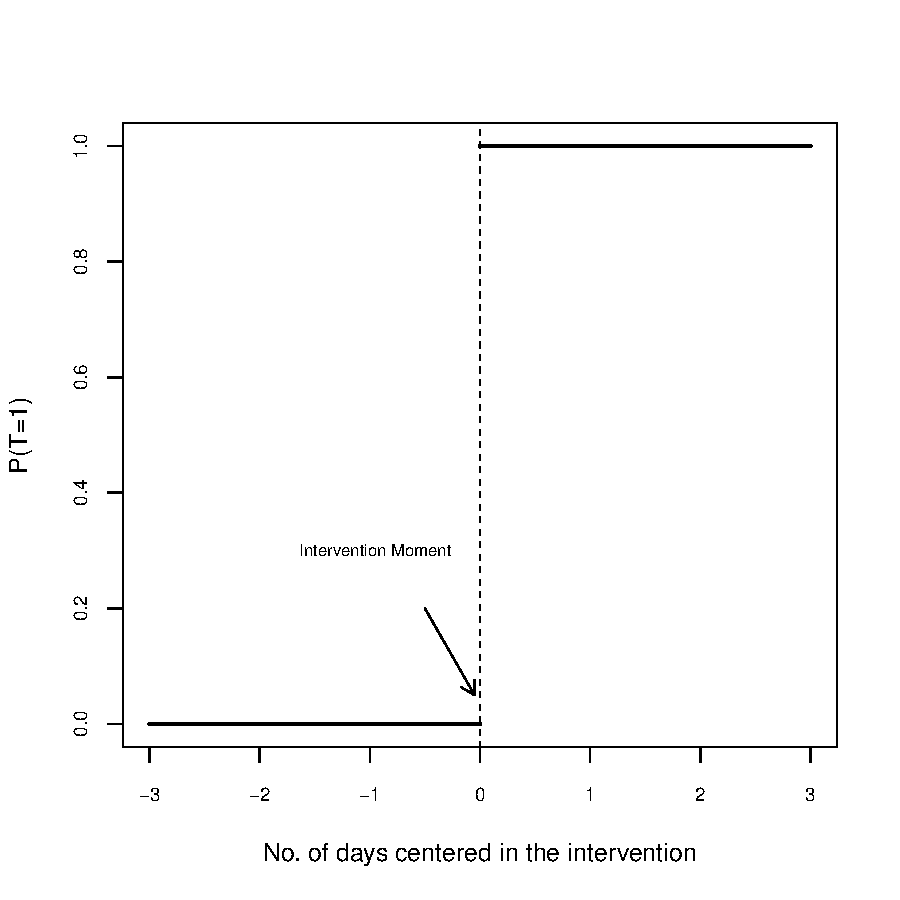
\includegraphics{TESE_DE_DOUTORADO_RENAN_FINAL-plot_exemp_inter}
\end{center}
\caption{Representation of a sharp intervention}
\label{fig:repre_inter_sharp}
\end{figure}

In terms of modeling, the equation below presents the model in its reduced form
\begin{align*}
Y_{da}=\beta_{0} + \tau I(T_{da}\geq 0)+g(T_{da})+X_{da}\beta + \varepsilon_{da}
\label{eq:mod_rdd}
\end{align*}
where $d$ represents the number of days after DST, $a$ represent years, $T_{da}$ is the horizontal axis variable (also referred as running variable), $X_{da}$ represents a vector of covariates, $g(\cdot)$ is a flexible function nonparametrically estimated, $Y_{da}$ is the dependent variable which, in this case, is the homicide rate per 100,000 inhabitants and $\tau$ represents the effect of DST discontinuity on the dependent variable and can be interpreted as the local effect of the treatment. As in \co{doleac2015} and \co{toro2016}, it is expected that the criminal rate falls more sharply in the hours most affected by the transition. Thus, models will be estimated by analyzing both the full day and the hours close to sunset (both before and after). Additionally, covariables will be included as the day of the week and climatological variables.

This type of discontinuity regression can be seen as a semiparametric model, being a particular case of the Generalized Additive Models (GAM) \cite{loeffler2015processed}. Thus, its equation will be estimated via GAM, where its nonparametric function of the $T$ variable will be estimated via local linear polynomial regression \textit{Loess} \cite{cleveland1988locally} with smoothing parameter equal to 0.5.

\subsection{Data Preparation\label{preparacao_dados_HV}}

Before presenting the results obtained, some considerations must be made regarding the data used in the study. Firstly, to control the possible idiosyncrasies of the data it is emphasized that models will be estimated with the inclusion of covariables, such as weekdays and daily climatological variables. In addition, this paper uses homicide rates as dependent variable, that is, it is already corrected by the size of the population. The climatological variables obtained on the INMET website are average temperature information\footnote{In the meteorological stations three temperature readings are made every six hours. For a perfect control, a fourth reading should be done, which is not usually the case. Thus, the average temperature that is calculated is not exactly the average of the day. What meteorologists do then is to calculate an average of the three readings, plus the maximum and the minimum. The average of these five values is called \textit{average temperature compensated} and this is the information used here.}, wind speed and pluviometric precipitation\footnote{Other variables were considered, but excluded due to excess of missing data.}. Considering that INMET presents data only for 19 municipalities where meteorological stations are present, the estimated values for RS represent a weighted average by the population of each of these municipalities.

Another important fact that is taken into account is that on the day that the DST begins, clocks must be advanced by one hour and in this sense the day ''loses'' one hour which could underestimate the number of homicide cases on the day immediately following the change in DST. To correct this possible distortion, the number of homicides occurring on this day is multiplied by 24/23\footnote{This correction is also made by \co{toro2016} although the results have been robust to it in their work.}. Similarly, when DST is terminated the number of deaths of the immediately subsequent day is multiplied by 23/24.

The variable that represents the number of days until the start (or end) of DST is constructed according to Table \ref{tab:HV_RS}.


\begin{table}[H]
\caption{DST dates implemented}
\begin{center}
\begin{small}
\begin{tabular}{cc}
\hline 
Season & Duration\\
\hline 
2005/2006 & from 0am of October 16, 2005, until 0am of February 19, 2006\tabularnewline
2006/2007 & from 0am of November 5, 2006, until 0am of February 25, 2007\tabularnewline
2007/2008 & from 0am of October 14, 2007, until 0am of February 17, 2008\tabularnewline
2008/2009 & from 0am of October 19, 2008, until 0am of February 15, 2009\tabularnewline
2009/2010 & from 0am of October 18, 2009, until 0am of February 21, 2010\tabularnewline
2010/2011 & from 0am of October 17, 2010, until 0am of February 20, 2011\tabularnewline
2011/2012 & from 0am of October 16, 2011, until 0am of February 26, 2012\tabularnewline
2012/2013 & from 0am of October 21, 2012, until 0am of February 17, 2013\tabularnewline
2013/2014 & from 0am of October 20, 2013, until 0am of February 16, 2014\tabularnewline
2014/2015 & from 0am of October 19, 2014, until 0am of February 22, 2015\tabularnewline
2015/2016 & from 0am of October 18, 2015, until 0am of February 21, 2016\tabularnewline
\hline
\multicolumn{2}{l}{Source: Elaborated by the author.}
\end{tabular}
\end{small}
\end{center}
\label{tab:HV_RS}
\end{table}


\section{Results\label{resultados_HV}}



\subsection{Descriptive Statistics\label{descritivas_HV}}

In this section we analyze some descriptive statistics of the SIM database for Rio Grande do Sul in the period between 2006 and 2014. Figure \ref{fig:taxas_homicidios_por_ano_RS} shows daily homicide rates per 100 thousand inhabitants stratified per year. We see that the values oscillate near 0.04 with some outliers surpassing the values of 0.12. In addition, there is no specific year that distinguishes itself from others in level terms. On the horizontal axis of each these graphs are the number of days in relation to the start day of DST (negative values for previous days and positive for later ones) and the dashed vertical line located at zero represents the first day of DST.

A pre-regression nonparametric line was included in each of the charts to check the trend of criminal rates. If there is a structural change between the period before and after the dashed lines, the nonparametric trend is expected to undergo a change as it traverses them, something that is not apparent when we analyze these raw data graphs. However, possible structural breaks may be present in the separate estimates between the two period segments (pre and post intervention).

\begin{figure}[H]
\begin{center}
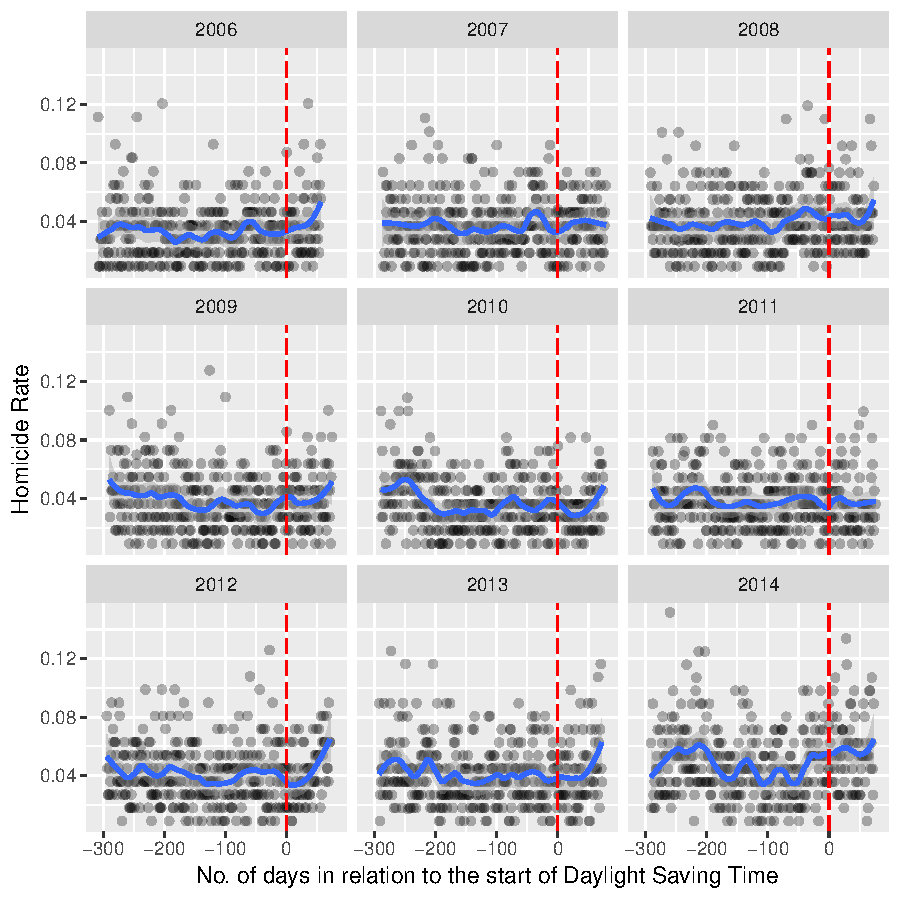
\includegraphics{TESE_DE_DOUTORADO_RENAN_FINAL-plot1_HV}
\end{center}
\caption{Homicide rates stratified per year in Rio Grande do Sul}
\source{Source: SIM and FEE-RS}
\label{fig:taxas_homicidios_por_ano_RS}
\end{figure}

When we do not distinguish per year from the series and analyze only the 80 days next to the entry of the DST (40 days before and 40 days later) the resulting graph is that represented in Figure \ref{fig:taxas_homicidios_por_ano_RS_empilhado_agrupando_Diff}. This graph illustrates the overall behavior of RS crime rates in the days close to the entry of DST without distinction of year, i.e., making the overall RS rate grouped by days. This visualization again does not make it clear if there is a structural break close to the zero day line.

\begin{figure}[H]
\begin{center}
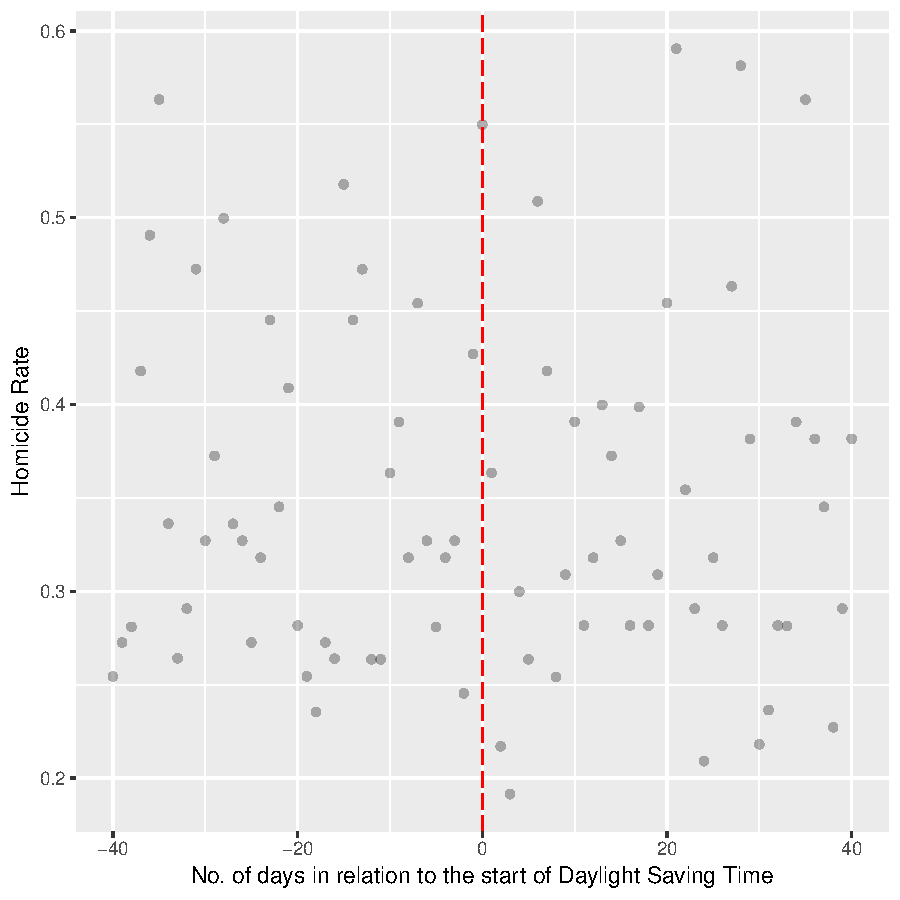
\includegraphics{TESE_DE_DOUTORADO_RENAN_FINAL-plot2_HV}
\end{center}
\caption{General homicide rates in Rio Grande do Sul only in a period close to the entry of Daylight Saving Time}
\source{Source: SIM and FEE-RS}
\label{fig:taxas_homicidios_por_ano_RS_empilhado_agrupando_Diff}
\end{figure}



An interesting aspect is to analyze the temporal location of homicide occurrences. More specifically, see where the biggest and smallest homicides occur in terms of months of the year, days of the week and times throughout the day. Regarding the months of the year, in Figure \ref{fig:meses_ano} we notice that the hottest months of the year like December, January, February and March have significantly higher rates than the mid-year months. In the descriptive analysis of the days of the week, it was observed that there is, significantly\footnote{Kruskal-Wallis nonparametric tests were performed with Dunn's multiple comparisons with $\alpha = 5\%$ to compare months of the year and days of the week. This test is analogous to Analysis of Variance (ANOVA) and was used because the residuals did not adhere to the normality hypothesis.}, a greater concentration of homicides on weekends (Saturday and Sunday), while the days that showed a lower degree of occurrence are midweek days such as Tuesday or Wednesday. The distribution of homicides on weekdays is well defined having high values on weekends followed by a gradual reduction to mid-week and then a gradual rise to arrive at the weekend again. Therefore, there is a ''day-of-the-week'' effect that must be included in the analysis. This effect is shown in Figure \ref{fig:dias_semana}.



\begin{figure}[H]
\begin{center}
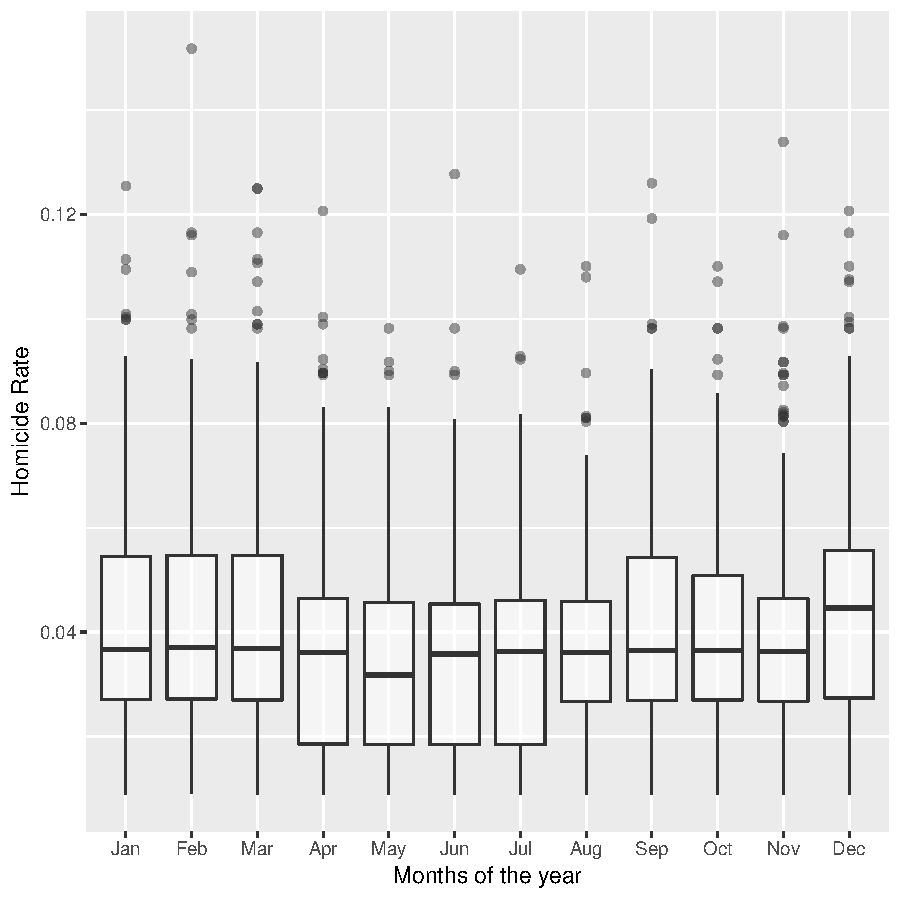
\includegraphics{TESE_DE_DOUTORADO_RENAN_FINAL-plot_meses_HV}
\end{center}
\caption{Homicide rates for months of the year in Rio Grande do Sul}
\source{Source: SIM and FEE-RS}
\label{fig:meses_ano}
\end{figure}



\begin{figure}[H]
\begin{center}
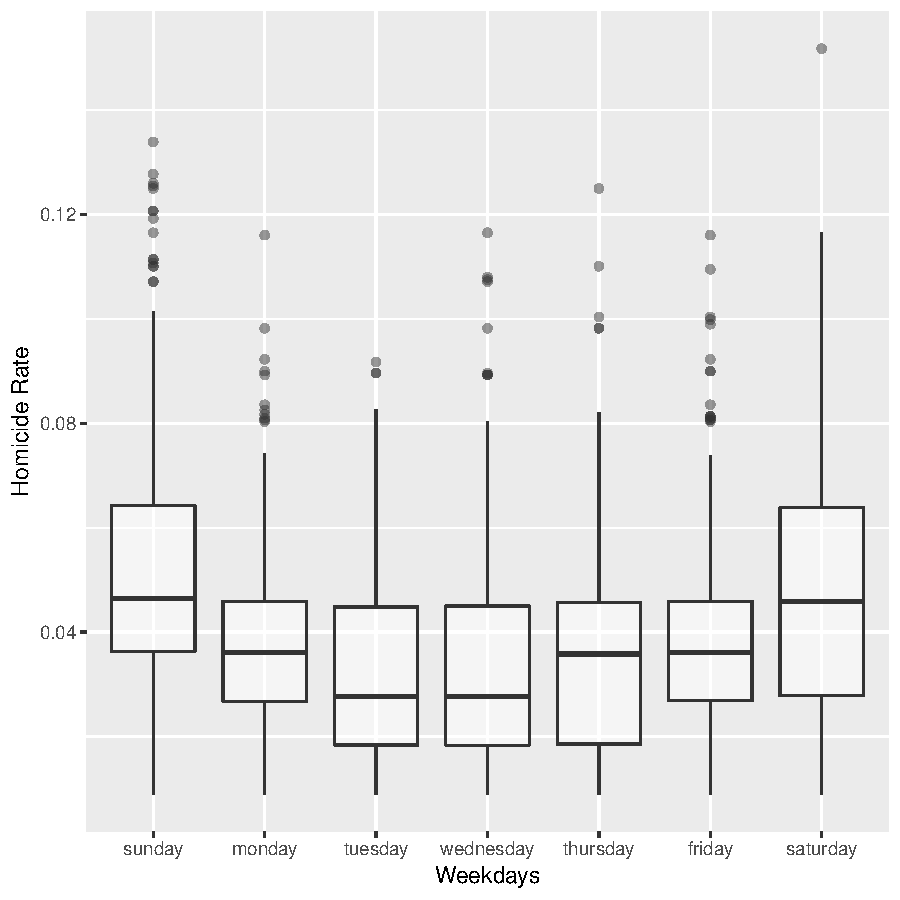
\includegraphics{TESE_DE_DOUTORADO_RENAN_FINAL-plot3_HV}
\end{center}
\caption{Homicide rates for days of the week in Rio Grande do Sul}
\source{Source: SIM and FEE-RS}
\label{fig:dias_semana}
\end{figure}


Regarding the death schedules, the distribution is quite interesting and Figure \ref{fig:horarios} shows the frequency of homicides that were recorded for every minute of the day of the entire study sample\footnote{Part of the sample (almost 0.3\%) was considered missing, since the death time field was not filled. In addition, we did not consider the deaths that presented the 00:00 time, placing them as missing as well.}. In this frequency chart,  it is highlighted with labels the times that presented values above 50 and it is possible to analyze that, except for the time of the first ten minutes of the morning, they are all well defined hours of the day, that is, are either complete hours or half an hour. With regard to the complete hours, stand out night schedules like 1am, 7pm, 8pm, 9pm, 10pm and 11pm. This type of behavior is in line with what was discussed in Section \ref{introdução_HV}, where an environment with poor clarity leads to delinquent behavior. This graph, therefore, corroborates the motivation of this paper.

In general, it is possible to note that the overall distribution tendency of homicide cases follows a smooth curve having a ''valley'' at hours close to noon and having two ''hills''. The first ''hill'' is represented by the hours of dawn having a peak in 1am, while the second ''hill'' is located in the hours of the end of the day having its peak at 22pm.

The complete hours have a high frequency and prominence in the graph. However, it is also possible to observe that, interspersed with complete hours, there are intermediate times appearing every half hour with a frequency pattern similar to full hours, where their highest values are at 8:30 p.m., 9:30 p.m., 10:30 p.m. and 11:30 p.m. This location pattern of most criminal occurrence draws attention to the fact that there might be a possible imprecision and knowledge of the exact time the murder occurred. It is reasonable to assume that the real distribution is somewhat smoother between minutes, but because of the ease and convenience of recording, more defined times are chosen for specific hours or half an hour between these times. Despite these caveats with respect to the data it is possible to visualize more ''broken'' times illustrated in small bars along the graph of Figure \ref{fig:horarios}.


\begin{figure}[H]
\begin{center}
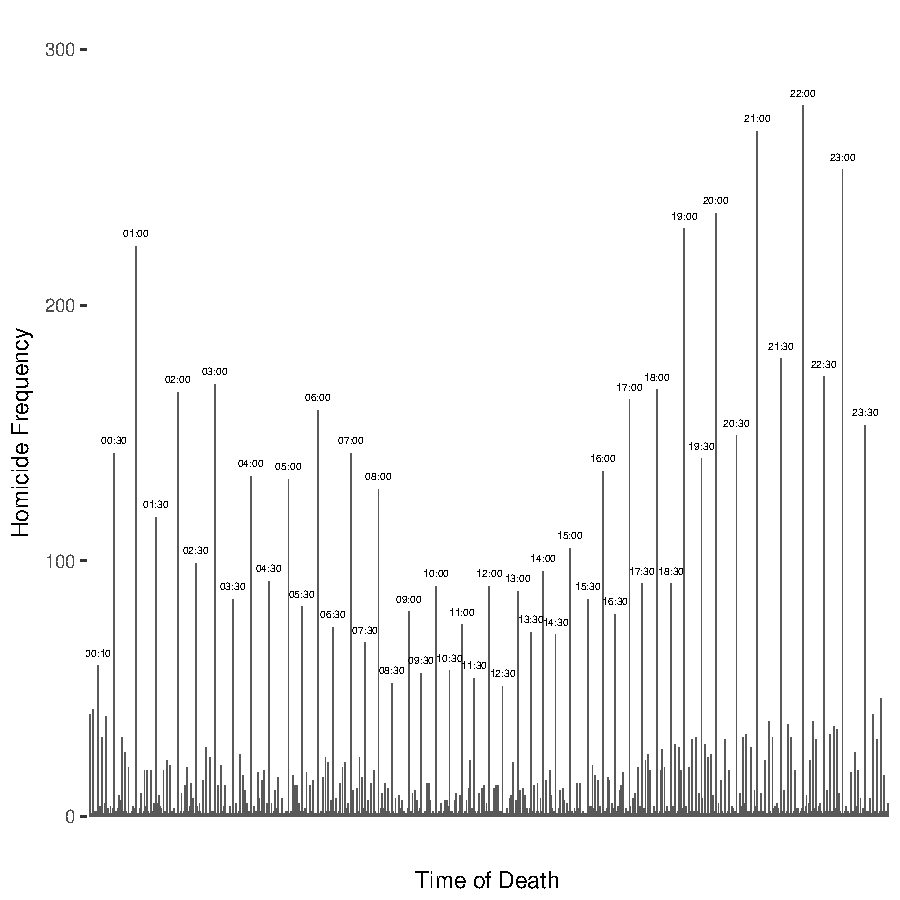
\includegraphics{TESE_DE_DOUTORADO_RENAN_FINAL-plot4_HV}
\end{center}
\caption{Homicide rates by time of occurrence in Rio Grande do Sul}
\source{Source: SIM and FEE-RS}
\label{fig:horarios}
\end{figure}

Through the INMET data it is possible to analyze if there is some kind of relation between criminal rates and climatic variables. The main variable that proved to be important in the homicidal relationship was the average temperature of the days \footnote{The graphs of the other variables can be found in Appendix \ref{appen:HV_clima_e_taxa}}. There is a clear trend that on warmer days, homicidal rates are higher as can be seen in Figure \ref{fig:temp_homicidios}. Most linear correlations were positive and significant ($\alpha = 5\%$).

\begin{figure}[H]
\begin{center}
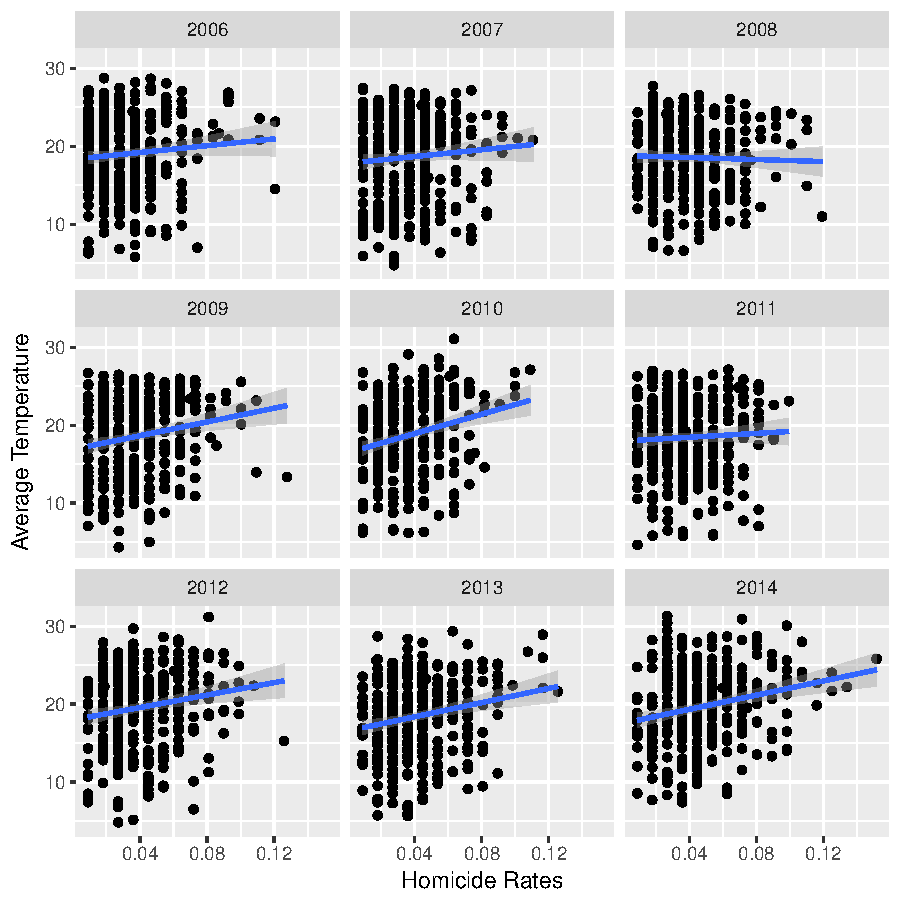
\includegraphics{TESE_DE_DOUTORADO_RENAN_FINAL-plot_temp_HV}
\end{center}
\caption{Homicide rates by average temperature in Rio Grande do Sul}
\source{Source: SIM, FEE-RS and INMET}
\label{fig:temp_homicidios}
\end{figure}

The relation of temperature to criminal behavior has already been discussed in some studies in the literature. \co{ranson2014crime} shows that, for US, there is a strong positive effect between monthly temperature and murder, rape, theft, vehicle theft, among others. \co{gamble2012temperature} verify that, for Dallas, the daily temperature had a strong relation with severe aggressions, being characterized by an inverted U with inflection point at 32.2°C. In addition, the authors found a similar relationship for sexual assaults and homicides, but not very explanatory. \co{britto2014analise} analyzes criminal data from Juiz de Fora (brazilian state of Minas Gerais) and several climatic variables, where the monthly temperature is related to death by homicide. For Pelotas (brazilian city of Rio Grande do Sul state), \co{silveira2000relaccao} analyze graphically the positive relation between the increase of the monthly temperature and the increase of the homicides.


\subsection{Regression Discontinuity - Start of DST\label{resultados_RDD_entrada}}

In this section we present the main results of the estimated RDDs for the DST entry period. The main models follow the structure similar to that described in Section \ref{reg_desc_HV}, being represented by two equations: one adding covariates and other not. Equation \ref{eq:mod_rdd_completo} represents the complete model

\begin{small}
\begin{equation}
HR_{da}=\beta_{0}+\tau I(T_{da}\geq 0)+g(T_{da})+\beta_{1}Temp_{da}+\beta_{2}Prec_{da}+\beta_{3}Wind_{da} + \beta_{k}Day_{dak} + \varepsilon_{da}
\label{eq:mod_rdd_completo}
\end{equation}
\end{small}
where $k = monday, tuesday, ..., saturday$ is the index of the day-of-week fixed effect ($sunday$ is the reference category), $d$ o index of the day and $a$ the year index, where each equation is estimated for each year separately. The dependent variable is $HR$ (homicide rate) and the covariates are abbreviated as $Temp$ (temperature), $Prec$ (pluviometric precipitation) and $Wind$ (wind speed). In addition, we estimate a model without covariates, according to Equation \ref{eq:mod_rdd_bruto}
\begin{equation}
HR_{da}=\beta_{0}+\tau I(T_{da}\geq 0)+g(T_{da}) + \varepsilon_{da}.
\label{eq:mod_rdd_bruto}
\end{equation}

With regard to DST entry, the main results are summarized in Table \ref{tab:resultados_taus_entrada_RS} and Figure \ref{fig:resultado_rdd_entrada}\footnote{It makes sense to take a look, previously, at the effect of possible discontinuity on covariates to justify their use in increasing the precision of $\tau$. These results can be seen in Appendix \ref{appen:HV_efeito_cov_clima_entrada} in Figures \ref{fig:efeito_descon_temp_entrada_RS}, \ref{fig:efeito_descon_prec_entrada_RS} and \ref{fig:efeito_descon_velo_entrada_RS}. According to them, we can see that there is little (or no) significant discontinuity effect of the DST entry in climate variables, except for a drop in temperature in 2006 (Sig. $\approx$ 0.0266), an increase in precipitation in 2006 (Sig. $\approx$ 0.0243), a fall in precipitation in 2014 (Sig. $\approx$ 0.0259) and an increase in wind speed in 2013 (Sig. $<$ 0.0001).}. In all years and models it was observed a high absence of significance with the exception for the model with no covariates in 2007 that showed some level of significance below $\alpha = 0.05$. The results of the discontinuity effect indicate that, for DST entry, there is neither increase nor drop in homicide rates indicating that, if any, it is due only to random fluctuations of the data. Only in 2007, there is an indication of the positive effect of DST on criminal rates of $\tau = 0.0195$, i.e., with an opposite direction than expected.


Figure \ref{fig:resultado_rdd_entrada} illustrates the main results of the nonparametric regressions between the period prior to the implementation of the DST (Pre Period) and the later period (Post Period) for the models without covariates. It is possible to verify that the local regression curves do not, in fact, show any signs of abrupt changes of direction when it crosses $T=0$. In addition, the 95\% confidence intervals between pre- and post-discontinuity period have a large intersection in values. In this figure, however, we can note the result consistent with the only significance found in the previous Table \ref{tab:resultados_taus_entrada_RS} for the year 2007. In the central upper chart, the nonparametric trend of the postintervention period goes up when $T = 0$ indicating an increase in the homicide rate soon after DST entry.


\begin{table}[H]
\caption{Local Effects of DST entry for all years and models}
\begin{center}
\begin{small}
\begin{tabular}{rrrc}
  \hline
Year & Effects ($\tau$) & Significance & Does it include covariates? \\ 
  \hline
2006 & 0.0116 & 0.1431 & Yes \\ 
2006 & 0.0134 & 0.1807 & No \\ 
2007 & 0.0175 & 0.0600 & Yes \\ 
2007 & 0.0195 & 0.0300 & No \\ 
2008 & 0.0046 & 0.6345 & Yes \\ 
2008 & 0.0060 & 0.5807 & No \\ 
2009 & -0.0043 & 0.6054 & Yes \\ 
2009 & -0.0034 & 0.6827 & No \\ 
2010 & -0.0077 & 0.3085 & Yes \\ 
2010 & -0.0029 & 0.6966 & No \\ 
2011 & 0.0000 & 0.9991 & Yes \\ 
2011 & 0.0012 & 0.8814 & No \\ 
2012 & -0.0084 & 0.3536 & Yes \\ 
2012 & -0.0090 & 0.3524 & No \\ 
2013 & -0.0010 & 0.9171 & Yes \\ 
2013 & -0.0004 & 0.9638 & No \\ 
2014 & 0.0041 & 0.6898 & Yes \\ 
2014 & 0.0095 & 0.4035 & No \\
   \hline
\multicolumn{4}{l}{Source: Elaborated by the author.}
\end{tabular}
\end{small}
\end{center}
\label{tab:resultados_taus_entrada_RS}
\end{table}

\begin{figure}[H]
\begin{center}
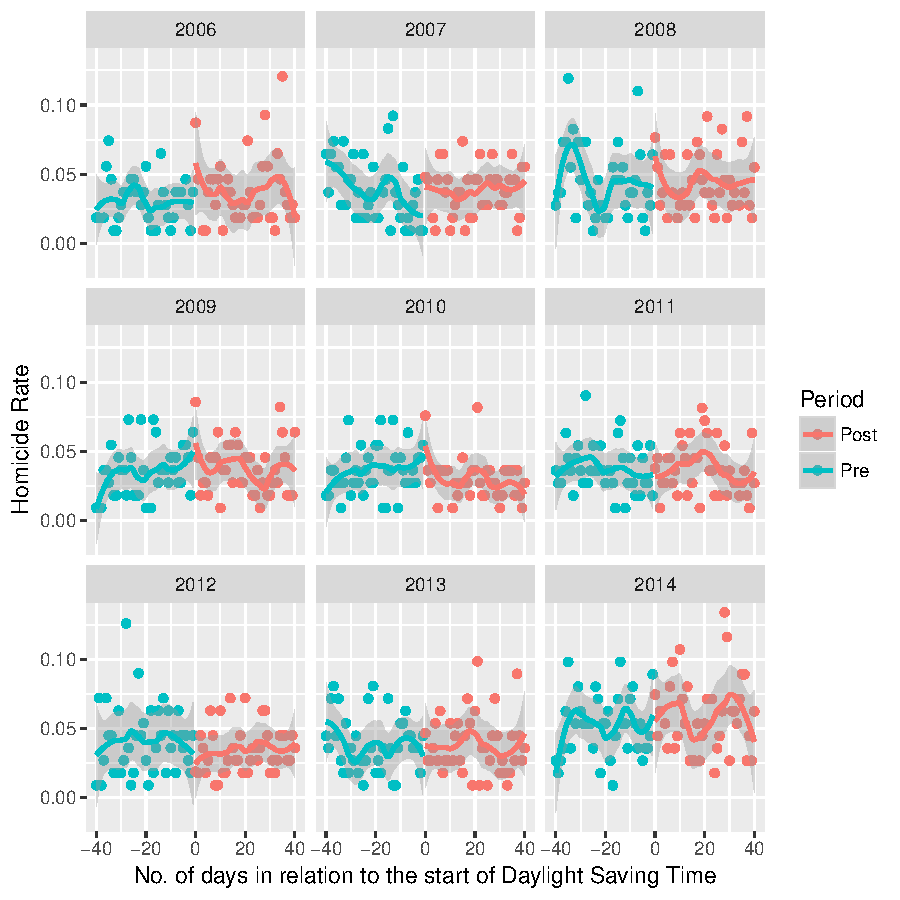
\includegraphics{TESE_DE_DOUTORADO_RENAN_FINAL-plot_resultados_rdd_entradaHV_RS}
\end{center}
\caption{Regression Discontinuity at the entrance of DST in models without covariables.}
\source{Source: Elaborated by the author, SIM and FEE-RS}
\label{fig:resultado_rdd_entrada}
\end{figure}




\begin{table}[H]
\caption{Effects of climate covariates every year and models at the entrance of DST}
\begin{center}
\begin{small}
\begin{tabular}{lrrr}
  \hline
Covariate & Year & Effects ($\beta$) & Significance \\ 
  \hline
Average Temperature &  2006 & 0.0018 & 0.0276 \\ 
Average Temperature &  2007 & 0.0009 & 0.2843 \\ 
Average Temperature &  2008 & 0.0005 & 0.6403 \\ 
Average Temperature &  2009 & 0.0004 & 0.6345 \\ 
Average Temperature &  2010 & 0.0001 & 0.9439 \\ 
Average Temperature &  2011 & -0.0009 & 0.3632 \\ 
Average Temperature &  2012 & 0.0008 & 0.4510 \\ 
Average Temperature &  2013 & 0.0023 & 0.0037 \\ 
Average Temperature &  2014 & 0.0033 & 0.0079 \\ 
Precipitation &  2006 & -0.0000 & 0.9857 \\ 
Precipitation &  2007 & 0.0001 & 0.7956 \\ 
Precipitation &  2008 & -0.0006 & 0.0784 \\ 
Precipitation &  2009 & -0.0002 & 0.2881 \\ 
Precipitation &  2010 & -0.0005 & 0.1405 \\ 
Precipitation &  2011 & 0.0005 & 0.1906 \\ 
Precipitation &  2012 & -0.0002 & 0.3666 \\ 
Precipitation &  2013 & -0.0002 & 0.2878 \\ 
Precipitation &  2014 & -0.0002 & 0.4200 \\ 
Wind Speed &  2006 & -0.0001 & 0.9835 \\ 
Wind Speed &  2007 & -0.0026 & 0.3864 \\ 
Wind Speed &  2008 & -0.0079 & 0.0408 \\ 
Wind Speed &  2009 & -0.0029 & 0.4033 \\ 
Wind Speed &  2010 & -0.0013 & 0.5763 \\ 
Wind Speed &  2011 & -0.0016 & 0.5165 \\ 
Wind Speed &  2012 & 0.0021 & 0.4672 \\ 
Wind Speed &  2013 & 0.0026 & 0.4367 \\ 
Wind Speed &  2014 & -0.0041 & 0.3464 \\
   \hline
\multicolumn{4}{l}{Source: Elaborated by the author.}
\end{tabular}
\end{small}
\end{center}
\label{tab:resultados_betas_entrada_RS}
\end{table}

Another interesting result to analyze is the relation of the climatic covariates in the regressions of the Model \ref{eq:mod_rdd_completo}. The Table \ref{tab:resultados_betas_entrada_RS} above shows all $\beta $ 's of all the years of temperature, precipitation and wind speed. Again, most of the effects are null, except for the average temperature that, in 2006, 2013 and 2014, was positively related to homicide rates. In addition, in 2008, there was an inverse effect between wind speed and rate, indicating that this year, as there was more wind in RS, there were fewer homicides (Sig. = 0.0408).

\begin{table}[H]
\caption{Weekdays effect on the entry of DST}
\begin{center}
\begin{tiny}
\begin{tabular}{lrrr}
  \hline
Covariate & Year & Coefficients & Significance \\ 
  \hline
  Monday &  2006 & -0.0243 & 0.0006 \\ 
  Tuesday &  2006 & -0.0412 & 0.0000 \\ 
  Wednesday &  2006 & -0.0407 & 0.0000 \\ 
  Thursday &  2006 & -0.0459 & 0.0000 \\ 
  Friday &  2006 & -0.0355 & 0.0000 \\ 
  Saturday &  2006 & -0.0226 & 0.0012 \\ 
  Monday &  2007 & 0.0041 & 0.6181 \\ 
  Tuesday &  2007 & -0.0120 & 0.1580 \\ 
  Wednesday &  2007 & -0.0147 & 0.0855 \\ 
  Thursday &  2007 & -0.0114 & 0.1728 \\ 
  Friday &  2007 & -0.0037 & 0.6555 \\ 
  Saturday &  2007 & 0.0036 & 0.6712 \\ 
  Monday &  2008 & -0.0307 & 0.0019 \\ 
  Tuesday &  2008 & -0.0347 & 0.0003 \\ 
  Wednesday &  2008 & -0.0454 & 0.0000 \\ 
  Thursday &  2008 & -0.0233 & 0.0106 \\ 
  Friday &  2008 & -0.0283 & 0.0028 \\ 
  Saturday &  2008 & -0.0115 & 0.2131 \\ 
  Monday &  2009 & -0.0066 & 0.4016 \\ 
  Tuesday &  2009 & -0.0143 & 0.0656 \\ 
  Wednesday &  2009 & -0.0216 & 0.0069 \\ 
  Thursday &  2009 & -0.0111 & 0.1571 \\ 
  Friday &  2009 & -0.0130 & 0.0965 \\ 
  Saturday &  2009 & 0.0041 & 0.5972 \\ 
  Monday &  2010 & -0.0086 & 0.2174 \\ 
  Tuesday &  2010 & -0.0096 & 0.1583 \\ 
  Wednesday &  2010 & -0.0144 & 0.0518 \\ 
  Thursday &  2010 & -0.0112 & 0.1070 \\ 
  Friday &  2010 & -0.0126 & 0.0697 \\ 
  Saturday &  2010 & -0.0117 & 0.0951 \\ 
  Monday &  2011 & -0.0202 & 0.0069 \\ 
  Tuesday &  2011 & -0.0259 & 0.0009 \\ 
  Wednesday &  2011 & -0.0185 & 0.0168 \\ 
  Thursday &  2011 & -0.0127 & 0.0781 \\ 
  Friday &  2011 & -0.0133 & 0.0651 \\ 
  Saturday &  2011 & -0.0138 & 0.0592 \\ 
  Monday &  2012 & -0.0171 & 0.0474 \\ 
  Tuesday &  2012 & -0.0308 & 0.0006 \\ 
  Wednesday &  2012 & -0.0115 & 0.1862 \\ 
  Thursday &  2012 & -0.0235 & 0.0070 \\ 
  Friday &  2012 & -0.0222 & 0.0096 \\ 
  Saturday &  2012 & -0.0063 & 0.4595 \\ 
  Monday &  2013 & -0.0245 & 0.0037 \\ 
  Tuesday &  2013 & -0.0198 & 0.0149 \\ 
  Wednesday &  2013 & -0.0167 & 0.0374 \\ 
  Thursday &  2013 & -0.0177 & 0.0278 \\ 
  Friday &  2013 & -0.0182 & 0.0279 \\ 
  Saturday &  2013 & -0.0035 & 0.6694 \\ 
  Monday &  2014 & -0.0187 & 0.0524 \\ 
  Tuesday &  2014 & -0.0362 & 0.0003 \\ 
  Wednesday &  2014 & -0.0309 & 0.0020 \\ 
  Thursday &  2014 & -0.0246 & 0.0107 \\ 
  Friday &  2014 & -0.0193 & 0.0450 \\ 
  Saturday &  2014 & -0.0095 & 0.3227 \\ 
   \hline
\multicolumn{4}{l}{Source: Elaborated by the author.} \\ 
\multicolumn{4}{l}{Obs.: sunday represents the reference category.}
\end{tabular}
\end{tiny}
\end{center}
\label{tab:resultados_efeito_dia_semana_entrada}
\end{table}

The weekday covariates were the ones that presented the most relevant in the model as previously discussed. The weekday effect is negative and significant in most of the $\beta$'s, indicating a Sunday homicide peak as seen in Table \ref{tab:resultados_efeito_dia_semana_entrada}.

A very important feature of the intervention, which can not be ignored, is that both the start and the end of DST, \textbf{always occur at dawn between Saturday and Sunday}. Moreover, we found that the day of the week has a considerable influence on criminal practice both in descriptive terms, as seen in Section \ref{descritivas_HV}, and in inferential terms as now analyzed in the effect of its covariate. However, we see in Table \ref{tab:resultados_efeito_dia_semana_entrada} that the effect of Saturday in relation to Sunday (illustrated by the coefficient of Saturday) is not so strong and, for the most part, it is not significant what indicates that there is a ''weekend effect'' in criminal activity. That is, there is a historical ''weekend'' discontinuity while DST will necessarily be confused with the ''Saturday vs. Sunday'' effect. Since the effect of the discontinuity of the regression is local and takes into account the neighborhood of the points the effect, ''Friday vs. Saturday'' locally affects the transition ''Saturday vs. Sunday''.









\subsection{Regression Discontinuity - End of DST\label{resultados_RDD_saida}}

In this section we present the results of DST ending\footnote{Previously, it makes sense to analyze the discontinuity effect on covariates as presented in the Appendix \ref{appen:HV_efeito_cov_clima_saida} in Figures \ref{fig:efeito_descon_temp_saida_RS}, \ref{fig:efeito_descon_prec_saida_RS} and \ref{fig:efeito_descon_velo_saida_RS}. In most of the models, there was no significance, but in other years these discontinuities deserve attention. In relation to temperature, we can see that in general there is a decreasing trend of temperature as leaving the summer. However, we see positive discontinuities with effect of 2.59 in 2007 (Sig. = 0.0033) and 1.54 in 2009 (Sig. = 0.0292). Regarding precipitation, we noticed a discontinuity of 5.42 in 2006 (Sig. = 0.0254) and -11.64 in 2007 (Sig. < 0,001). The wind speed presented discontinuity in 2006 (0,53 with Sig. = 0.0375), 2009 (-0,499 with Sig. = 0.0355) and 2013 (0,7565 with Sig. = 0.0154).}. Table \ref{tab:resultados_taus_saida_RS} and Figure \ref{fig:resultado_rdd_saida} illustrate the main results of this approach.

% Chuva forte de 2007: http://intelog.net/site/default.asp?TroncoID=907492&SecaoID=508074&SubsecaoID=948063&Template=../artigosnoticias/user_exibir.asp&ID=821702&Titulo=Deslizamento%20bloqueia%20RS-470


\begin{table}[H]
\caption{Local Effects of DST ending for all years and models}
\begin{center}
\begin{small}
\begin{tabular}{rrrc}
  \hline
Year & Effects ($\tau$) & Significance & Does it include covariates? \\
  \hline
2006 & -0.0039 & 0.6746 & Yes \\ 
2006 & 0.0051 & 0.6176 & No \\ 
2007 & 0.0129 & 0.1983 & Yes \\ 
2007 & 0.0096 & 0.3610 & No \\ 
2008 & -0.0132 & 0.1825 & Yes \\ 
2008 & -0.0070 & 0.4690 & No \\ 
2009 & -0.0143 & 0.0880 & Yes \\ 
2009 & -0.0088 & 0.3622 & No \\ 
2010 & -0.0130 & 0.2104 & Yes \\ 
2010 & -0.0125 & 0.1933 & No \\ 
2011 & 0.0058 & 0.4814 & Yes \\ 
2011 & 0.0077 & 0.3804 & No \\ 
2012 & 0.0073 & 0.3544 & Yes \\ 
2012 & 0.0091 & 0.3198 & No \\ 
2013 & -0.0374 & 0.0002 & Yes \\ 
2013 & -0.0346 & 0.0007 & No \\ 
2014 & 0.0092 & 0.4569 & Yes \\ 
2014 & 0.0057 & 0.6194 & No \\ 
   \hline
\multicolumn{4}{l}{Source: Elaborated by the author.}
\end{tabular}
\end{small}
\end{center}
\label{tab:resultados_taus_saida_RS}
\end{table}


\begin{figure}[H]
\begin{center}
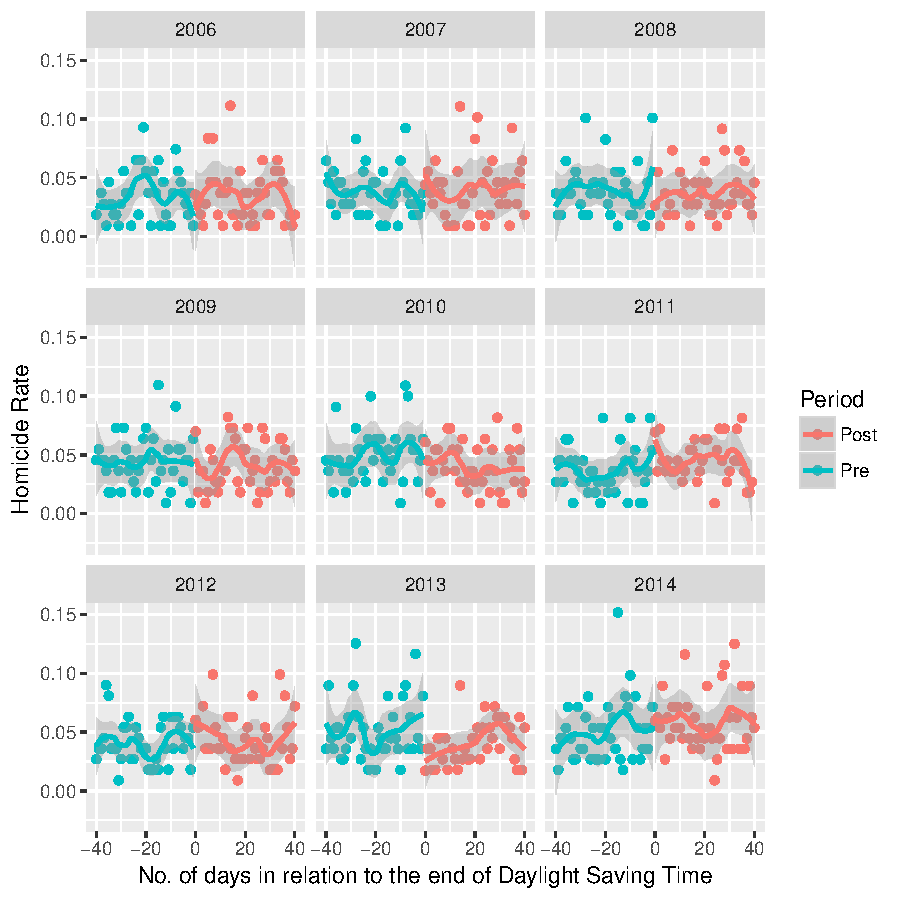
\includegraphics{TESE_DE_DOUTORADO_RENAN_FINAL-plot_resultados_rdd_saidaHV_RS}
\end{center}
\caption{Regression Discontinuity at the end of DST in models without covariates.}
\source{Source: Elaborated by the author, SIM and FEE-RS}
\label{fig:resultado_rdd_saida}
\end{figure}



Analyzing the Table \ref{tab:resultados_taus_saida_RS} there is absence again of statistical significance in all the years of the series. Virtually all effects estimated for $\tau$ do not have any statistical evidence indicating discontinuity, with the exception of the year 2013. This year we saw that we had the negative effect of $\tau = -0.0374$ for the model with covariates and $\tau = -0.0346$ for the simplest model. What draws attention, again, to this result is that the direction of the effect is the opposite of what is expected. The intervention of leaving the DST implies less light during the day which would lead to an increase in the homicide rate, which was not the case. In addition, it should be considered that, in Table \ref{fig:efeito_descon_velo_saida_RS} of the Appendix \ref{appen:HV_efeito_cov_clima_saida}, we see that this year there was an abrupt increase in wind speed just at the exit of the DST. Therefore, this effect of reducing crime may be confused with increasing wind speed, since we have seen that these two variables can be related according to the already discussed results of the Table \ref{tab:resultados_betas_entrada_RS}.


\begin{table}[H]
\caption{Effects of climate covariates every year and models at the exit of DST}
\begin{center}
\begin{small}
\begin{tabular}{lrrr}
  \hline
Covariate & Year & Effects ($\beta$) & Significance \\ 
  \hline
Average Temperature &  2006 & 0.0005 & 0.6170 \\ 
Average Temperature &  2007 & -0.0009 & 0.4997 \\ 
Average Temperature &  2008 & 0.0001 & 0.9697 \\ 
Average Temperature &  2009 & 0.0015 & 0.2317 \\ 
Average Temperature &  2010 & 0.0006 & 0.6115 \\ 
Average Temperature &  2011 & 0.0012 & 0.4340 \\ 
Average Temperature &  2012 & 0.0021 & 0.0149 \\ 
Average Temperature &  2013 & -0.0010 & 0.3618 \\ 
Average Temperature &  2014 & 0.0016 & 0.2261 \\ 
Precipitation &  2006 & 0.0007 & 0.1345 \\ 
Precipitation &  2007 & 0.0003 & 0.3719 \\ 
Precipitation &  2008 & -0.0004 & 0.3438 \\ 
Precipitation &  2009 & 0.0004 & 0.1528 \\ 
Precipitation &  2010 & -0.0001 & 0.7302 \\ 
Precipitation &  2011 & 0.0003 & 0.4314 \\ 
Precipitation &  2012 & 0.0001 & 0.7556 \\ 
Precipitation &  2013 & 0.0001 & 0.7448 \\ 
Precipitation &  2014 & 0.0003 & 0.4796 \\ 
Wind Speed &  2006 & 0.0096 & 0.0313 \\ 
Wind Speed &  2007 & 0.0021 & 0.6430 \\ 
Wind Speed &  2008 & 0.0043 & 0.2200 \\ 
Wind Speed &  2009 & -0.0026 & 0.5229 \\ 
Wind Speed &  2010 & 0.0023 & 0.5931 \\ 
Wind Speed &  2011 & 0.0020 & 0.6016 \\ 
Wind Speed &  2012 & -0.0021 & 0.5401 \\ 
Wind Speed &  2013 & 0.0028 & 0.4402 \\ 
Wind Speed &  2014 & 0.0057 & 0.1960 \\ 
   \hline
\multicolumn{4}{l}{Source: Elaborated by the author.}
\end{tabular}
\end{small}
\end{center}
\label{tab:resultados_betas_saida_RS}
\end{table}

The effect of the covariates on the end of DST is summarized in Table \ref{tab:resultados_betas_saida_RS}. Only Temperature in 2012 ($\beta = 0.0021$ e Sig. = 0.0149) and Wind Speed in 2006 ($\beta = 0.0096$ e Sig. = 0.0313) showed significant results. Again, there is evidence that as temperatures rise, criminal rates increase as well. On the other hand, the Wind Speed result indicates that, in 2006, as there is more wind, higher homicide rates occur.


\begin{table}[H]
\caption{Weekdays effect on the end of DST}
\begin{center}
\begin{tiny}
\begin{tabular}{lrrr}
  \hline
Covariate & Year & Coefficients & Significance \\
  \hline
  Monday &  2006 & -0.0227 & 0.0078 \\ 
  Tuesday &  2006 & -0.0315 & 0.0003 \\ 
  Wednesday &  2006 & -0.0369 & 0.0001 \\ 
  Thursday &  2006 & -0.0183 & 0.0273 \\ 
  Friday &  2006 & -0.0159 & 0.0541 \\ 
  Saturday &  2006 & -0.0097 & 0.2565 \\ 
  Monday &  2007 & -0.0255 & 0.0070 \\ 
  Tuesday &  2007 & -0.0289 & 0.0024 \\ 
  Wednesday &  2007 & -0.0293 & 0.0028 \\ 
  Thursday &  2007 & -0.0159 & 0.0945 \\ 
  Friday &  2007 & -0.0312 & 0.0011 \\ 
  Saturday &  2007 & -0.0135 & 0.1416 \\ 
  Monday &  2008 & -0.0143 & 0.1046 \\ 
  Tuesday &  2008 & -0.0226 & 0.0123 \\ 
  Wednesday &  2008 & -0.0214 & 0.0178 \\ 
  Thursday &  2008 & -0.0176 & 0.0467 \\ 
  Friday &  2008 & -0.0159 & 0.0692 \\ 
  Saturday &  2008 & -0.0025 & 0.7712 \\ 
  Monday &  2009 & -0.0160 & 0.0381 \\ 
  Tuesday &  2009 & -0.0230 & 0.0027 \\ 
  Wednesday &  2009 & -0.0141 & 0.0588 \\ 
  Thursday &  2009 & -0.0267 & 0.0008 \\ 
  Friday &  2009 & -0.0262 & 0.0008 \\ 
  Saturday &  2009 & 0.0115 & 0.1275 \\ 
  Monday &  2010 & -0.0014 & 0.8814 \\ 
  Tuesday &  2010 & -0.0058 & 0.5140 \\ 
  Wednesday &  2010 & -0.0088 & 0.3278 \\ 
  Thursday &  2010 & -0.0202 & 0.0273 \\ 
  Friday &  2010 & -0.0148 & 0.1084 \\ 
  Saturday &  2010 & 0.0058 & 0.5207 \\ 
  Monday &  2011 & -0.0254 & 0.0017 \\ 
  Tuesday &  2011 & -0.0236 & 0.0027 \\ 
  Wednesday &  2011 & -0.0284 & 0.0005 \\ 
  Thursday &  2011 & -0.0199 & 0.0096 \\ 
  Friday &  2011 & -0.0135 & 0.0795 \\ 
  Saturday &  2011 & -0.0126 & 0.1106 \\ 
  Monday &  2012 & -0.0064 & 0.3860 \\ 
  Tuesday &  2012 & -0.0201 & 0.0091 \\ 
  Wednesday &  2012 & -0.0244 & 0.0014 \\ 
  Thursday &  2012 & -0.0200 & 0.0091 \\ 
  Friday &  2012 & -0.0201 & 0.0078 \\ 
  Saturday &  2012 & 0.0006 & 0.9344 \\ 
  Monday &  2013 & -0.0155 & 0.0921 \\ 
  Tuesday &  2013 & -0.0237 & 0.0107 \\ 
  Wednesday &  2013 & -0.0029 & 0.7496 \\ 
  Thursday &  2013 & -0.0216 & 0.0190 \\ 
  Friday &  2013 & -0.0147 & 0.1035 \\ 
  Saturday &  2013 & -0.0010 & 0.9161 \\ 
  Monday &  2014 & -0.0260 & 0.0210 \\ 
  Tuesday &  2014 & -0.0170 & 0.1194 \\ 
  Wednesday &  2014 & -0.0178 & 0.1006 \\ 
  Thursday &  2014 & -0.0123 & 0.2545 \\ 
  Friday &  2014 & -0.0167 & 0.1238 \\ 
  Saturday &  2014 & 0.0029 & 0.7910 \\
   \hline
\multicolumn{4}{l}{Source: Elaborated by the author.} \\ 
\multicolumn{4}{l}{Obs.: sunday represents the reference category.}
\end{tabular}
\end{tiny}
\end{center}
\label{tab:resultados_efeito_dia_semana_saida}
\end{table}

The effects of the weekdays at the exit of DST are in the Table \ref{tab:resultados_efeito_dia_semana_saida} and their indications are analogous to those discussed in Section \ref{resultados_RDD_entrada}. It is possible to note that the ''weekend'' effect remains present since Saturday's $\beta$'s are not significant and weekdays have significant negative effect for most of the values.

In general, these results of the end of DST only confirm the main results found for the start period. That is, without evidence that DST has an influence on crime. In terms of model results with covariables, it was observed that in both cases, weekend effects are strong and there is evidence of a positive relationship between temperature and homicide in some years (especially in start models for DST).


\section{Robustness Checks\label{resultados_robustez}}

The results found do not indicate a significant effect in many of the cases of DST in homicide rates. This section is devoted to evaluating the method used under different estimation techniques. 

\subsection{Estimation with \textit{demean} approach\label{robustez_demean}}

The first robustness check is given by the nature of the variable $Y$ to be estimated in the discontinuity regression. The demean method used in \co{smith2016} and \co{toro2016} seeks to remove the possible confounding effects of the method by correcting the dependent variable by making $Y$ the logarithm of the value adjusted by the mean of homicides occurred on that day of the week, in that specific region and in that specific year\footnote{This method adjusts the number of homicides \textit{on each day of the week in each region in each year} by the average number of homicides occurred on that day of the week, in that region and in that specific year. For example, the dependent variable for, to say, the Monday following the DST transition in the state of RS in the year of 2008 is the logarithm of the number of homicides on that Monday in RS divided by the average number of homicides occurred during all the Mondays of 2008 in RS.}. In this case, there would be no need to include weekday covariates nor the need to estimate separate models per year, but it would make the use of climatic covariates unfeasible. In this sense, the model to be estimated follows the Equation \ref{eq:mod_rdd_bruto}.

Figures \ref{fig:entrada_HV_demean} and \ref{fig:saida_HV_demean} present the graphical and inferential results using this approach. In both results, we again verified the non-significance of the DST effect for both start and end models. This result is in line with the findings of this study, indicating that there is no effect of DST on homicides in RS.




% - Modelos RS e somente com conjunto de municípios (sendo só no apêndice)


\begin{figure}[H]
\begin{center}
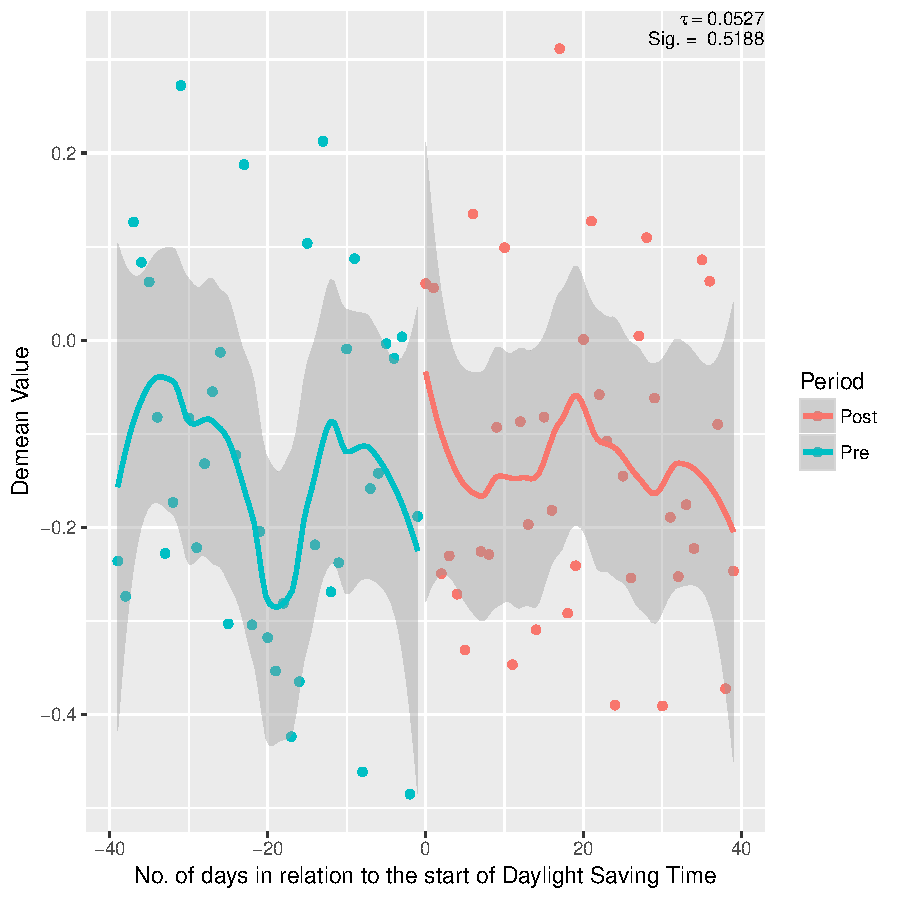
\includegraphics{TESE_DE_DOUTORADO_RENAN_FINAL-plot_entrada_demean_pelo_GAM}
\end{center}
\caption{Start of DST with \textit{demean} method}
\source{Source: Elaborated by the author, SIM and FEE-RS}
\label{fig:entrada_HV_demean}
\end{figure}





\begin{figure}[H]
\begin{center}
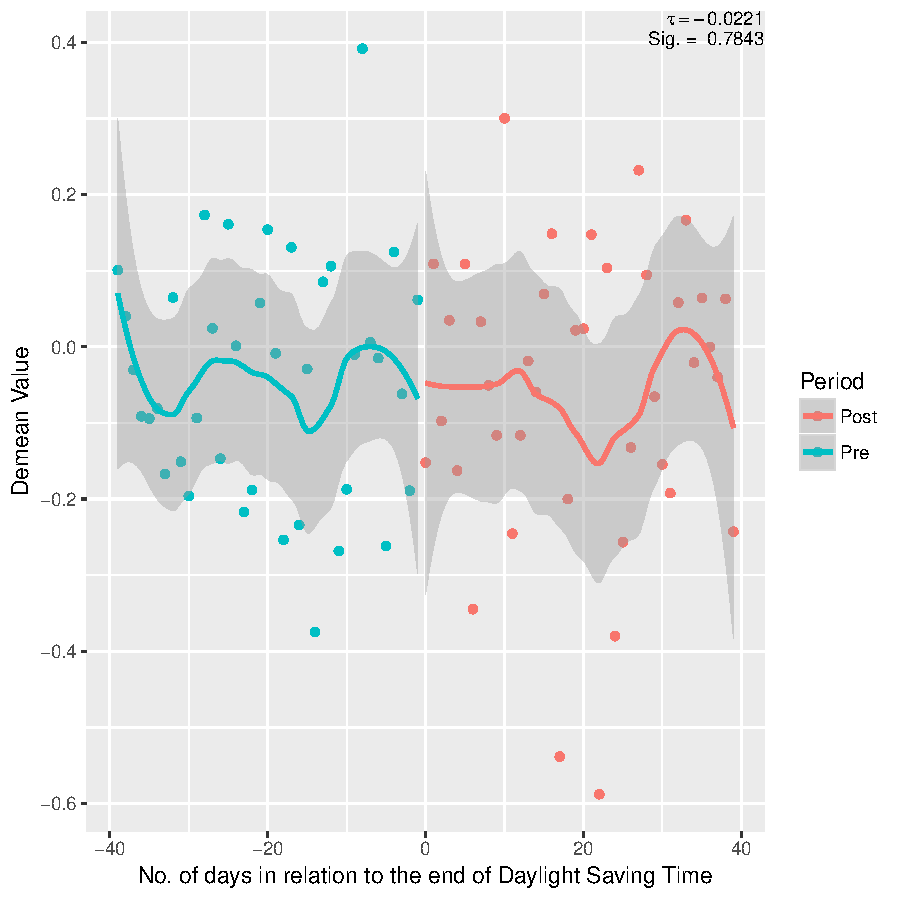
\includegraphics{TESE_DE_DOUTORADO_RENAN_FINAL-plot_saida_demean_pelo_GAM}
\end{center}
\caption{End of DST with \textit{demean} method}
\source{Source: Elaborated by the author, SIM and FEE-RS}
\label{fig:saida_HV_demean}
\end{figure}

\subsection{\textit{Bandwidth} choice\label{robustez_bandwidth_alternativa}}

One of the components of nonparametric estimation is the choice of the smoothing parameter (or \textit{bandwidth}) in the local regression. \co{calonico2014robust} discuss robust ways of estimating discontinuity regressions, as well as proposing alternative \textit{bandwidths}. Using the authors' approach, we estimated the start and end models of DST\footnote{We highlight that, for this, it was necessary to make use of the \textbf{rdrobust} package presented and described in \co{calonico2015rdrobust} in software R \cite{softwareR}, where the optimal \textit{bandwidth} used in this section minimizes the mean squared error. In Section \ref{resultados_HV}, the estimation was performed using Generalized Additives Models and the package \textbf{gam} \cite{gamPackage} was used because with it the marginal effects of covariates could be analyzed.}.

Tables \ref{tab:resultados_entrada_bandwidth_alternativa} and \ref{tab:resultados_saida_bandwidth_alternativa} show the results of the effect of DST ($\tau$) on start and end models. Although there was a larger set of significance, the changes were not very substantial since, again, in virtually all models and years there was no significant effect of $\tau$. The biggest highlights of the entry are in 2006, 2010 and 2013 for models with covariates. Regarding the end of DST in Table \ref{tab:resultados_saida_bandwidth_alternativa}, this \textit{bandwidth} pointed out some interesting significance as an increase in the homicide rate in 2007 in both models and a reduction in the rate in 2013 in line with the results previously presented.

\begin{table}[H]
\caption{Results of DST entry using alternative bandwidth}
\begin{center}
\begin{small}
\begin{tabular}{rrrc}
  \hline
Year & Effects ($\tau$) & Significance & Does it include covariates? \\ 
  \hline
2006 & 0.0404 & 0.0001 & Yes \\ 
2006 & 0.0242 & 0.3121 & No \\ 
2007 & 0.0088 & 0.5503 & Yes \\ 
2007 & 0.0287 & 0.0764 & No \\ 
2008 & 0.0125 & 0.0563 & Yes \\ 
2008 & 0.0254 & 0.3210 & No \\ 
2009 & -0.0112 & 0.2031 & Yes \\ 
2009 & 0.0062 & 0.8225 & No \\ 
2010 & -0.0145 & 0.0273 & Yes \\ 
2010 & 0.0012 & 0.9505 & No \\ 
2011 & -0.0033 & 0.6611 & Yes \\ 
2011 & -0.0017 & 0.9028 & No \\ 
2012 & 0.0044 & 0.5971 & Yes \\ 
2012 & -0.0046 & 0.7194 & No \\ 
2013 & 0.0187 & 0.0004 & Yes \\ 
2013 & 0.0130 & 0.3171 & No \\ 
2014 & 0.0172 & 0.0730 & Yes \\ 
2014 & -0.0042 & 0.8693 & No \\
   \hline
\multicolumn{4}{l}{Source: Elaborated by the author.}
\end{tabular}
\end{small}
\end{center}
\label{tab:resultados_entrada_bandwidth_alternativa}
\end{table}


\begin{table}[H]
\caption{Results of DST end using alternative bandwidth}
\begin{center}
\begin{small}
\begin{tabular}{rrrc}
  \hline
Year & Effects ($\tau$) & Significance & Does it include covariates? \\ 
  \hline
  2006 & 0.0690 & 0.0097 & Yes \\ 
  2006 & 0.0192 & 0.2072 & No \\ 
  2007 & 0.0545 & 0.0000 & Yes \\ 
  2007 & 0.0332 & 0.0006 & No \\ 
  2008 & -0.1228 & 0.0000 & Yes \\ 
  2008 & -0.0463 & 0.2834 & No \\ 
  2009 & 0.0134 & 0.3403 & Yes \\ 
  2009 & 0.0133 & 0.6456 & No \\ 
  2010 & -0.0234 & 0.0001 & Yes \\ 
  2010 & -0.0131 & 0.3561 & No \\ 
  2011 & 0.0029 & 0.6365 & Yes \\ 
  2011 & -0.0101 & 0.5902 & No \\ 
  2012 & -0.0040 & 0.6762 & Yes \\ 
  2012 & 0.0255 & 0.0867 & No \\ 
  2013 & -0.0264 & 0.0104 & Yes \\ 
  2013 & -0.0404 & 0.0507 & No \\ 
  2014 & -0.0059 & 0.4047 & Yes \\ 
  2014 & 0.0057 & 0.6762 & No \\
   \hline
\multicolumn{4}{l}{Source: Elaborated by the author.}
\end{tabular}
\end{small}
\end{center}
\label{tab:resultados_saida_bandwidth_alternativa}
\end{table}


\subsection{Most affected hours by the DST\label{robustez_horas_mais_afetadas}}

One of the main hypotheses raised in \co{doleac2015} and \co{toro2016} is that DST has a more pronounced effect in the hours closer to the transition between day and night, that is, in the hours closer to sunset. In these works, there is evidence that the effects are greater at times close to sunset. In this sense, it is also of interest to verify if this hypothesis holds for the case of RS\footnote{The time considered as close to sunset is between 17pm and 21pm}.

Figures \ref{fig:entrada_HV_demean_horas_mais_afetadas} and \ref{fig:saida_HV_demean_horas_mais_afetadas} show the results of the entry and exit, respectively, of the DST by the \textit{demean} method making use of only the cases that happened near the sunset. In the period of entry, again, we see no significant effect on the transition. However, in the case of exit we observed weak but nonsignificant (Sig. = 0.0668) evidence that there was an increase in homicide rate, which is in the sense of the main hypothesis of this article that less light indicates an increase in delinquency practice.

\begin{figure}[H]
\begin{center}
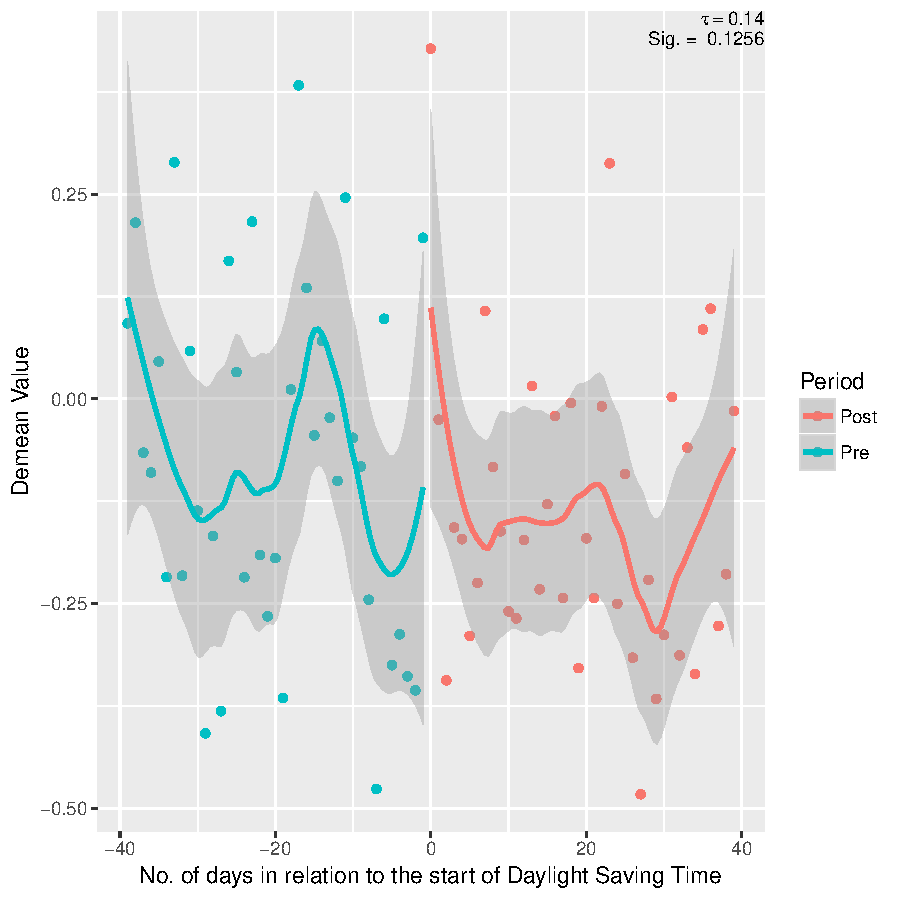
\includegraphics{TESE_DE_DOUTORADO_RENAN_FINAL-plot_entrada_demean_pelo_GAM_horas_mais_afetadas}
\end{center}
\caption{Entry of the DST with \textit{demean} method - Most affected hours}
\source{Source: Elaborated by the author, SIM and FEE-RS}
\label{fig:entrada_HV_demean_horas_mais_afetadas}
\end{figure}


\begin{figure}[H]
\begin{center}
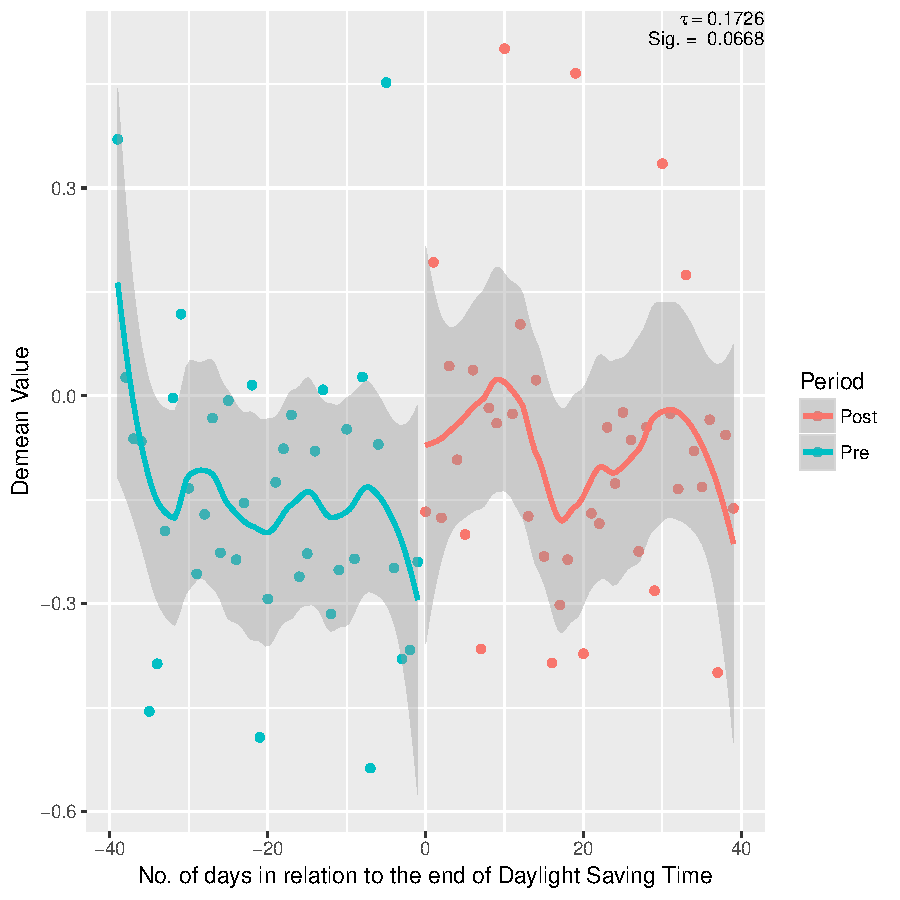
\includegraphics{TESE_DE_DOUTORADO_RENAN_FINAL-plot_saida_demean_pelo_GAM_horas_mais_afetadas}
\end{center}
\caption{End of the DST with \textit{demean} method - Most affected hours}
\source{Source: Elaborated by the author, SIM and FEE-RS}
\label{fig:saida_HV_demean_horas_mais_afetadas}
\end{figure}


\subsection{Analysis at all death occurrence location\label{robustez_todos_casos}}

In Section \ref{fonte_de_dados_HV}, it is described that the models are estimated only in cases where the death occurred outside hospitals and other health facilities implying a loss of 27.54\% of cases. Such treatment is due to the fact that it is possible that there is a reallocation of the day between the criminal occurrence and the time of death, something that is undesirable in this article considering the character of daily analysis of the local effect of DST. However, it is possible to assume that this loss of sample will affect the estimated results of this paper.

In this sense, this Section \ref{robustez_todos_casos} is dedicated to presenting the results taking into account the whole universe of homicides of the base of the SIM independent of the place of criminal occurrence. It is noteworthy that between 2006 and 2014 this entire base results in 19,318 cases.

Tables \ref{tab:resultados_taus_entrada_RS_TODOS_LOCAIS} and \ref{tab:resultados_taus_saida_RS_TODOS_LOCAIS} show the local effects of DST taking into account all cases of the database regardless of the place of occurrence. For the start models in the DST, again we did not identify any substantial changes in relation to the absence of significance of the Table \ref{tab:resultados_taus_entrada_RS}, except that with this approach the year of 2010 (with covariates) showed a significant reduction and not in the year of 2007 (without covariates) as seen previously. Regarding the end of the DST, the consonance with the results obtained is even greater, because, again, only the year of 2013 had a significant reduction in the models in the same way as was discussed in Section \ref{resultados_RDD_saida}.

\begin{table}[H]
\caption{Local effects of the DST start for all years and models - All occurrence locations}
\begin{center}
\begin{small}
\begin{tabular}{rrrc}
  \hline
Year & Effects ($\tau$) & Significance & Does it include covariates? \\
  \hline
2006 & 0.0041 & 0.6962 & Yes \\ 
2006 & 0.0053 & 0.6621 & No \\ 
2007 & 0.0036 & 0.7122 & Yes \\ 
2007 & 0.0061 & 0.5361 & No \\ 
2008 & -0.0034 & 0.7700 & Yes \\ 
2008 & 0.0020 & 0.8825 & No \\ 
2009 & -0.0070 & 0.4778 & Yes \\ 
2009 & -0.0026 & 0.7923 & No \\ 
2010 & -0.0221 & 0.0134 & Yes \\ 
2010 & -0.0147 & 0.1198 & No \\ 
2011 & 0.0016 & 0.8427 & Yes \\ 
2011 & 0.0034 & 0.6857 & No \\ 
2012 & -0.0014 & 0.8846 & Yes \\ 
2012 & -0.0007 & 0.9471 & No \\ 
2013 & -0.0029 & 0.7828 & Yes \\ 
2013 & -0.0020 & 0.8539 & No \\ 
2014 & 0.0018 & 0.8759 & Yes \\ 
2014 & 0.0072 & 0.5599 & No \\ 
   \hline
\multicolumn{4}{l}{Source: Elaborated by the author.}
\end{tabular}
\end{small}
\end{center}
\label{tab:resultados_taus_entrada_RS_TODOS_LOCAIS}
\end{table}


\begin{table}[H]
\caption{Local effects of the DST end for all years and models - All occurrence locations}
\begin{center}
\begin{small}
\begin{tabular}{rrrc}
  \hline
Year & Effects ($\tau$) & Significance & Does it include covariates? \\ 
  \hline
2006 & 0.0007 & 0.9465 & Sim \\ 
2006 & 0.0071 & 0.5742 & Não \\ 
2007 & 0.0120 & 0.2709 & Sim \\ 
2007 & 0.0121 & 0.3227 & Não \\
2008 & -0.0192 & 0.0901 & Yes \\ 
2008 & -0.0137 & 0.2676 & No \\ 
2009 & 0.0003 & 0.9765 & Yes \\ 
2009 & 0.0053 & 0.6663 & No \\ 
2010 & -0.0176 & 0.2050 & Yes \\ 
2010 & -0.0176 & 0.1851 & No \\ 
2011 & -0.0010 & 0.9155 & Yes \\ 
2011 & 0.0011 & 0.9102 & No \\ 
2012 & -0.0097 & 0.2710 & Yes \\ 
2012 & -0.0068 & 0.4835 & No \\ 
2013 & -0.0406 & 0.0008 & Yes \\ 
2013 & -0.0341 & 0.0052 & No \\ 
2014 & 0.0153 & 0.2643 & Yes \\ 
2014 & 0.0119 & 0.3832 & No \\
   \hline
\multicolumn{4}{l}{Source: Elaborated by the author.}
\end{tabular}
\end{small}
\end{center}
\label{tab:resultados_taus_saida_RS_TODOS_LOCAIS}
\end{table}




\section{Final Considerations\label{discussoes_e_consideracoes}}

The purpose of this article was to study the effect of the entry and exit of Daylight Saving Time (DST) on homicides in the Brazilian state of Rio Grande do Sul. The idea was to verify if the increase of the luminosity, caused by the entrance in the DST, has deterrent effect criminal. There is strong evidence in this sense that most homicides occur under darkness, peaking at 10 o'clock persisting until early morning hours, indicating that aggressors prefer to act during the nighttime period.

Using the brazilian Mortality Information System (SIM) homicide data, which has date and time information of the event, this study evaluated the effect of a possible discontinuity in the criminal activity both at the beginning and end of DST in the period 2006-2014. Under the hypothesis of lightening deterrence, it was expected that at the beginning of DST, there would be a drop in the homicide rate and, at the end of it, an increase.

The approach used Regression Discontinuity Design (RDD) in which nonparametric models are estimated for the pre- and post-intervention period and assess whether the local effect of transition from DST intervention is significant. In addition, the idiosyncrasies of the data are contemplated as the inclusion of fixed effect of day of the week, climatological covariables and separate estimations per year of each model.

The results showed that DST, in general, has no effect on the homicide rate. It was evidenced that in almost all the years of the historical series the effect of the DST was null with regard to the change in the level of the homicide rate. Besides, in some cases the results that were significant pointed in the \textbf{opposite-to-expected} sense, such as in 2007 that there was an increase in homicides when DST was started and in 2013 that there was a reduction in homicides when the DST ended\footnote{Possible confounding effect with wind speed.}. In this sense, although there is strong evidence that there is a luminosity effect on criminal activity when we analyze the hours of the day the homicides occur, it is not captured by the model when we analyze the effect of DST alone. One of the hypotheses to be considered for this lack of effect is that, although the change in DST time is sudden, the presence of ''more'' light during the day is actually gradual and in interstices, which mitigates the \textit{sharp} effect of the discontinuous intervention.

It is important to note that many variables affect delinquency behavior. History of behavioral problems in childhood \cite{murray2015childhood}, use of alcohol \cite{mcbride1991prediction, dearden2009alcohol} and social inequality \cite{kelly2000inequality,fajnzylber2002inequality}, for example, are factors that can influence criminal activity. Specifically, it is of interest to carry out future studies regarding the relationship between alcohol consumption and homicides for RS. In the analyzes presented here, we find that weekday plays a crucial role in criminal rates, where the weekend is when more crimes happen. In addition, strong evidence of a positive correlation between temperature and homicides was estimated.

The results estimated in this article were robust to variations of model specifications. Alternative approaches were tested such as the use of the demean method for estimation of RDD, alternative smoothing parameters, estimation for only those cases that occurred at hours more affected by DST and not excluding occurrences in hospitals and health facilities. In almost all situations, this intervention did not have a good explanatory power in the change of homicide rates.

This article advances considerably in the literature on the economics of crime because of its pioneering character of local evaluation of the DST effect on RS crimes. Up to the present time, no work is known that addressed this topic in the state. The discussion of the effects of DST is extremely relevant because it is a public policy that affects all the inhabitants of a certain place and studies that evaluate its true impact on the most different aspects are important to subsidize the public authorities to think/rethink this measure and its consequences in society. In 2017, the Brazilian federal government studied the possibility of excluding DST from the national calendar claiming that its main purpose of energy saving is not achieved\footnote{http://www1.folha.uol.com.br/cotidiano/2017/09/1920372-governo-avalia-se-ira-ou-nao-adotar-horario-de-verao-neste-ano.shtml - Accessed in october, 5th, 2017.}\footnote{https://g1.globo.com/distrito-federal/noticia/governo-federal-diz-que-estuda-extinguir-o-horario-de-verao-entenda.ghtml - Accessed in october, 5th, 2017.}, considering also to carry out popular consultation to evaluate its revocation\footnote{http://economia.estadao.com.br/noticias/geral,governo-fara-enquete-sobre-o-fim-do-horario-de-verao,70002010546 - Accessed in october, 5th, 2017.}. In this sense, studies like this one carried out are justified.



\begin{subappendices}
\chapter*{Appendix}
\addcontentsline{toc}{chapter}{Appendix}
\section{Relationship between climatic variables and homicide rates\label{appen:HV_clima_e_taxa}}

\begin{figure}[H]
\begin{center}
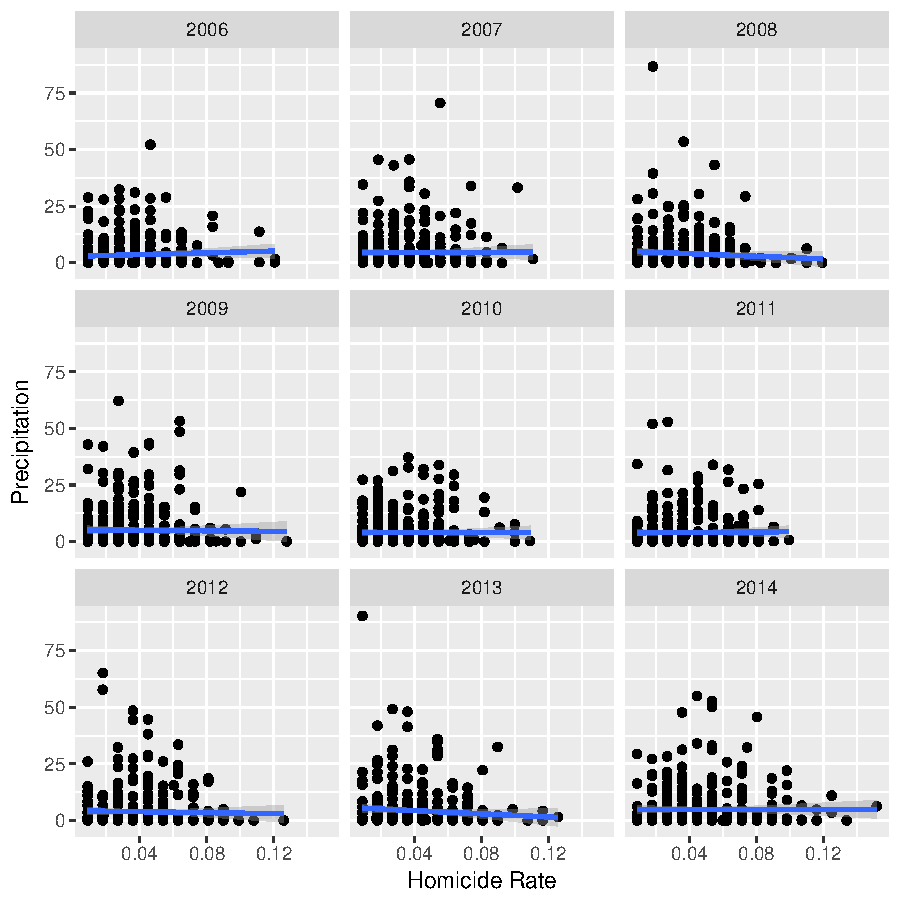
\includegraphics{TESE_DE_DOUTORADO_RENAN_FINAL-plot_prec_HV}
\end{center}
\caption{Homicide rate and pluviometric precipitation in Rio Grande do Sul}
\source{Source: SIM, FEE-RS and INMET}
\label{fig:prec_homicidios}
\end{figure}

\begin{figure}[H]
\begin{center}
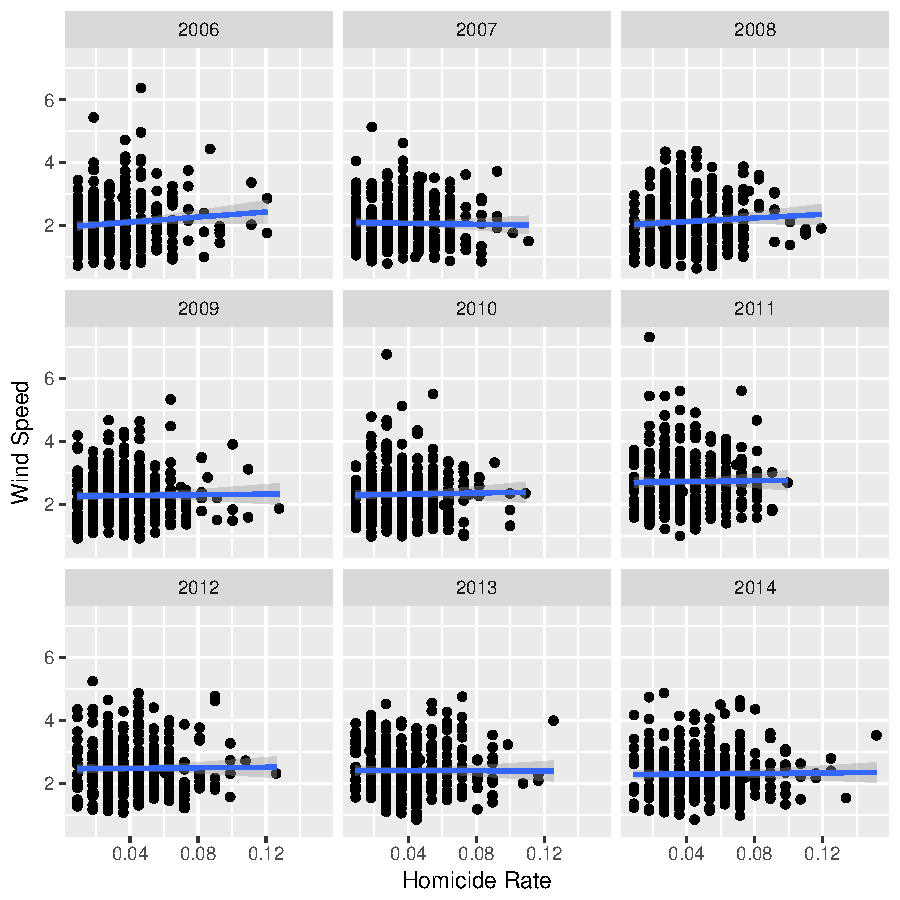
\includegraphics{TESE_DE_DOUTORADO_RENAN_FINAL-plot_veloc_HV}
\end{center}
\caption{Homicide rate and wind speed in Rio Grande do Sul}
\source{Source: SIM, FEE-RS and INMET}
\label{fig:veloc_homicidios}
\end{figure}


\section{Discontinuity Effects on Climate Covariates - Start of the DST\label{appen:HV_efeito_cov_clima_entrada}}

\begin{figure}[H]
\begin{center}
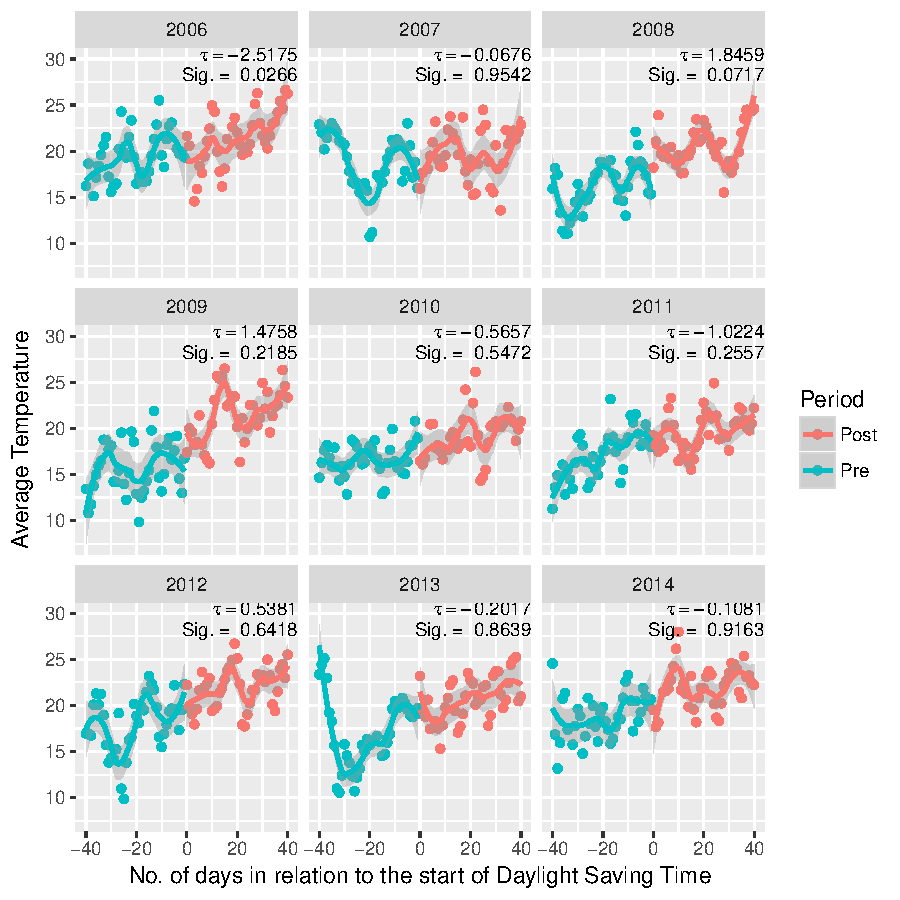
\includegraphics{TESE_DE_DOUTORADO_RENAN_FINAL-plot_efeito_descontinuo_temp_entrada}
\end{center}
\caption{Effect of temperature discontinuity at the start of the DST in RS}
\source{Source: SIM, FEE-RS and INMET}
\label{fig:efeito_descon_temp_entrada_RS}
\end{figure}

\begin{figure}[H]
\begin{center}
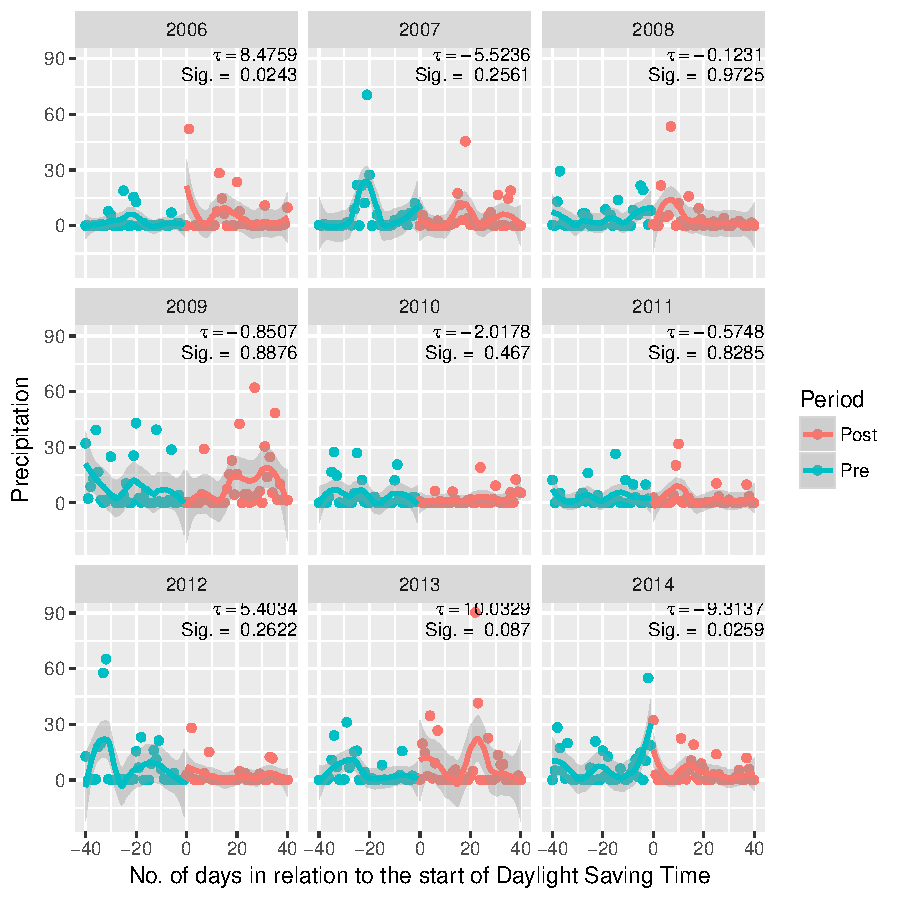
\includegraphics{TESE_DE_DOUTORADO_RENAN_FINAL-plot_efeito_descontinuo_prec_entrada}
\end{center}
\caption{Effect of pluviometric precipitation discontinuity at the start of the DST in RS}
\source{Source: SIM, FEE-RS and INMET}
\label{fig:efeito_descon_prec_entrada_RS}
\end{figure}


\begin{figure}[H]
\begin{center}
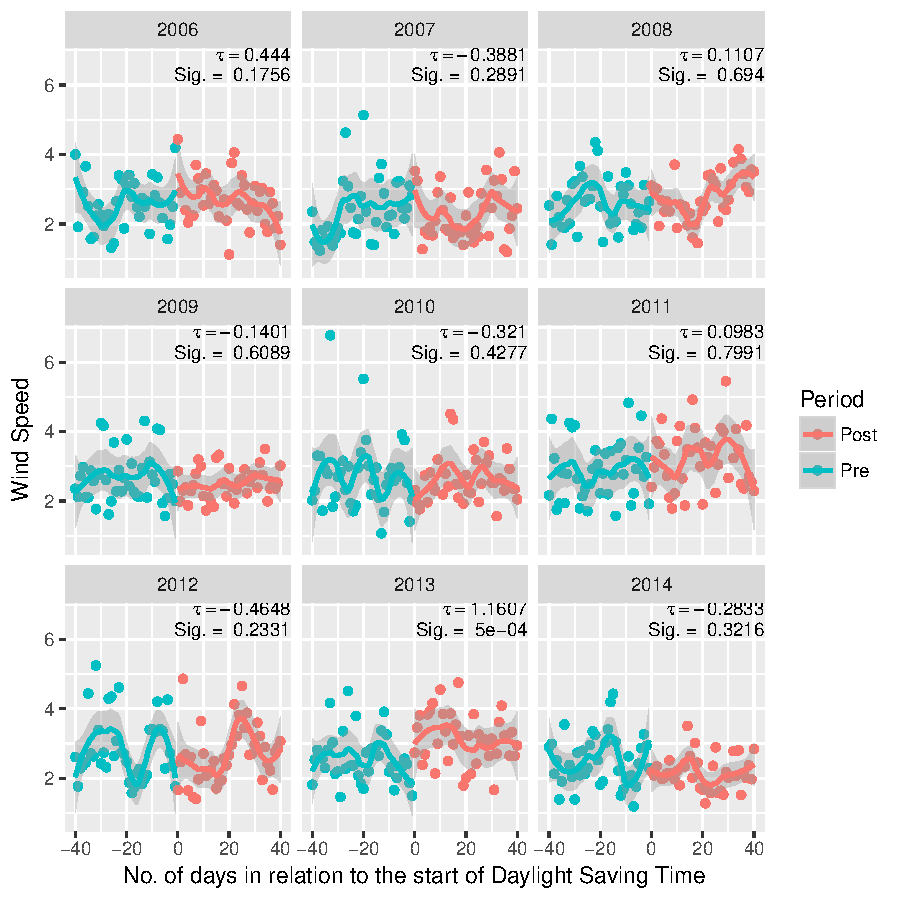
\includegraphics{TESE_DE_DOUTORADO_RENAN_FINAL-plot_efeito_descontinuo_velocidade_entrada}
\end{center}
\caption{Effect of wind speed at the start of the DST in RS}
\source{Source: SIM, FEE-RS and INMET}
\label{fig:efeito_descon_velo_entrada_RS}
\end{figure}

%\section{Efeitos do Dia da Semana - Entrada do HV\label{appen:HV_efeito_dia_semana_entrada}}






\section{Discontinuity Effects on Climate Covariates - End of the DST\label{appen:HV_efeito_cov_clima_saida}}

\begin{figure}[H]
\begin{center}
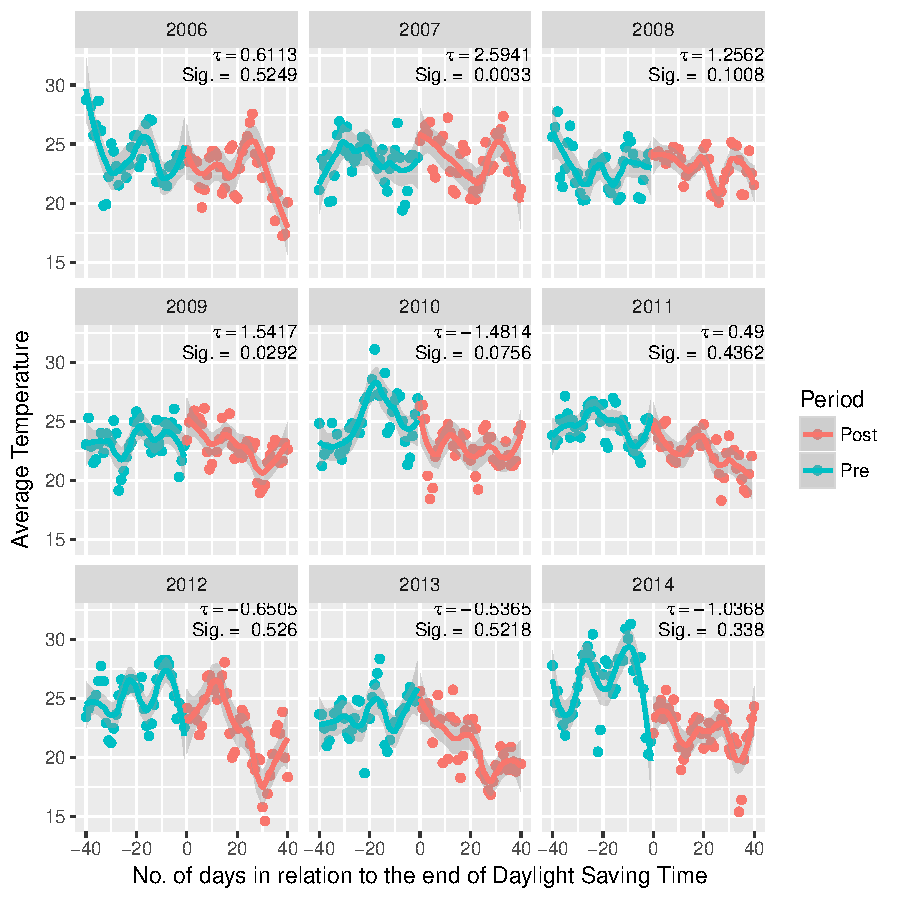
\includegraphics{TESE_DE_DOUTORADO_RENAN_FINAL-plot_efeito_descontinuo_temp_saida}
\end{center}
\caption{Effect of temperature discontinuity at the end of the DST in RS}
\source{Source: SIM, FEE-RS and INMET}
\label{fig:efeito_descon_temp_saida_RS}
\end{figure}


\begin{figure}[H]
\begin{center}
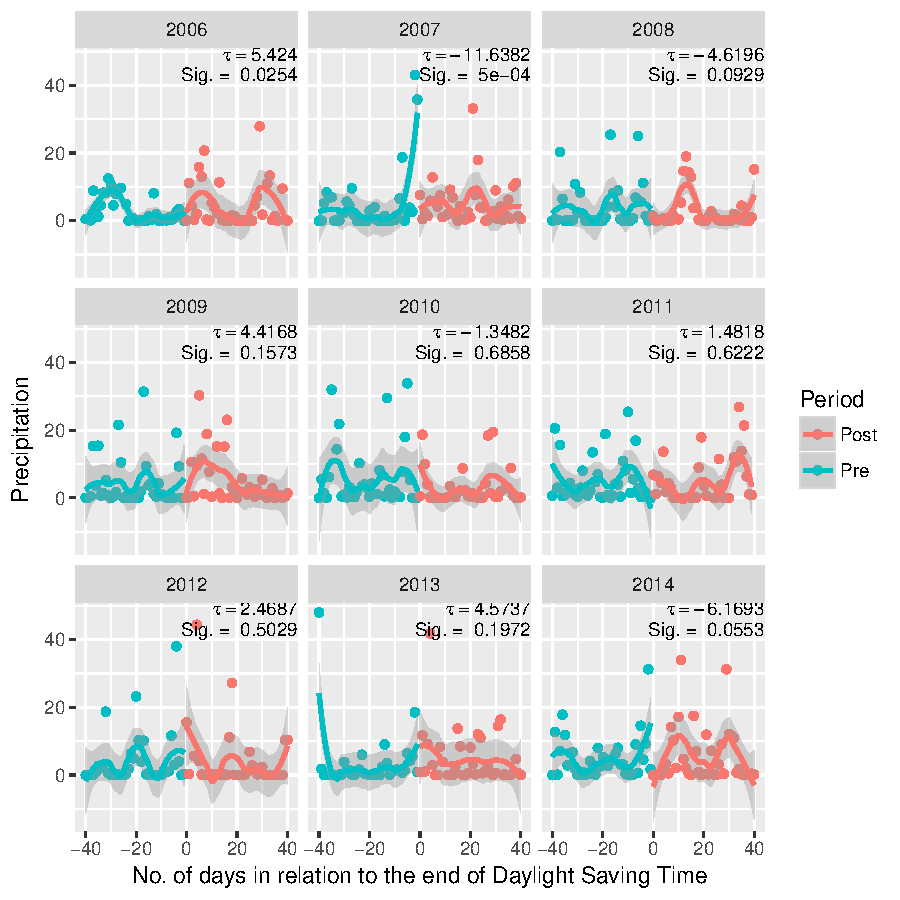
\includegraphics{TESE_DE_DOUTORADO_RENAN_FINAL-plot_efeito_descontinuo_prec_saida}
\end{center}
\caption{Effect of pluviometric precipitation discontinuity at the end of the DST in RS}
\source{Source: SIM, FEE-RS and INMET}
\label{fig:efeito_descon_prec_saida_RS}
\end{figure}


\begin{figure}[H]
\begin{center}
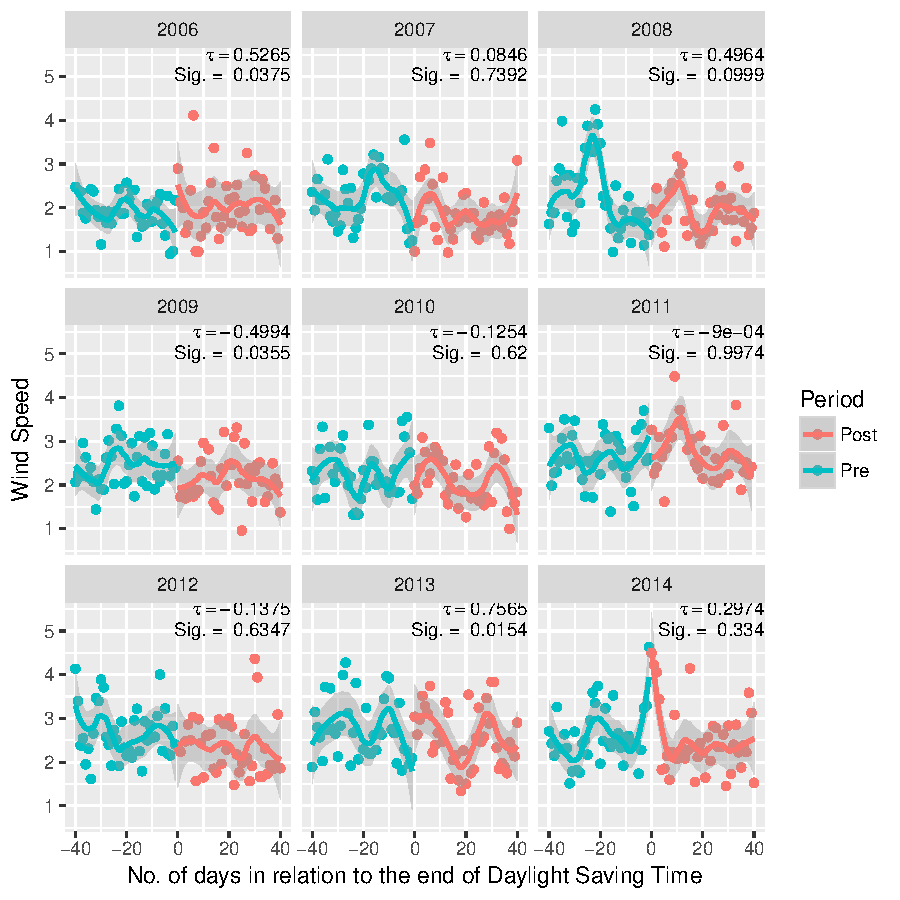
\includegraphics{TESE_DE_DOUTORADO_RENAN_FINAL-plot_efeito_descontinuo_velocidade_saida}
\end{center}
\caption{Effect of wind speed discontinuity at the end of the DST in RS}
\source{Source: SIM, FEE-RS and INMET}
\label{fig:efeito_descon_velo_saida_RS}
\end{figure}



\end{subappendices}

\end{otherlanguage}





\chapter{CrimeVis: uma ferramenta de visualização de dados de criminalidade}

\section{Introdução\label{sec:Introducao_CrimeVis}}

Este artigo tem como objetivo a construção de um aplicativo de visualização de dados \textit{CrimeVis}\footnote{O aplicativo foi desenvolvido pelo autor e está hospedado em http://visualiza.fee.tche.br/crime - Acesso em 22/10/2017}. Além disto, este artigo se propõe a discutir a importância da visualização de dados para compreender a dinâmica criminal no Rio Grande do Sul (RS).

A visualização de dados sempre desempenhou um papel muito importante na exploração de padrões inesperados em conjuntos de dados. Diversos artigos e trabalhos discutem a visualização de dados como \co{cleveland1984graphical}, \co{van2005value}, \co{mccandless2009information}. Em linhas gerais, a visualização de dados é um mecanismo de auxílio para o entendimento de um determinado fenômeno. Padrões, tendências e correlações, que podem estar indetectáveis nos dados brutos, podem ser expostos e reconhecidos facilmente com a visualização humana. Segundo \co{van2005value}, ela possibilita que pesquisadores, analistas, engenheiros e o público em geral obtenha \textit{insights} de uma maneira eficiente e efetiva, graças às exclusivas capacidades do sistema visual humano, que permite detectar padrões interessantes no curto prazo.

Adicionalmente, a inspeção visual deve fazer parte da modelagem de dados, uma vez que equações matemáticas e estatísticas de resumo podem esconder padrões não usuais de informações. Um exemplo muito interessante na literatura é o Quarteto de Anscombe \cite{anscombe1973graphs} que representa um conjunto de dados de duas variáveis que aparentam ser idênticos quando se usa estatísticas descritivas e regressão linear conforme a Figura \ref{fig:anscombe}.

% Para fazer este gráfico é necessário o pacote subcaption lá em cima
\begin{figure}[H]
\begin{center}
\begin{subfigure}{.55\textwidth}
  \centering
  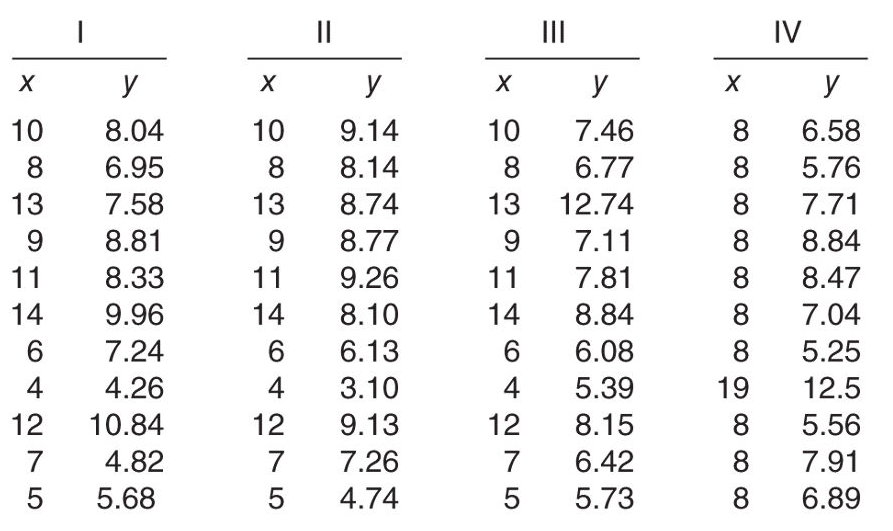
\includegraphics[width=.75\linewidth]{anscombe_dataset.png}
  \caption{Conjuntos de Dados}
  \label{fig:anscombe_data}
\end{subfigure} \\ % Quebra a linha para fazer os gráficos na vertical
\vspace{0.5cm} % Inclui um espaço em branco entre as figuras
\begin{subfigure}{.75\textwidth}
  \centering
  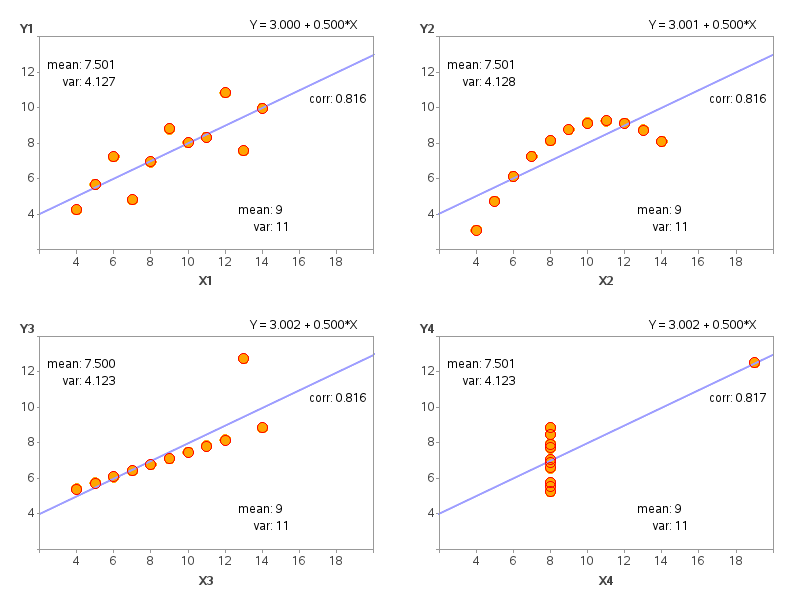
\includegraphics[width=.95\linewidth]{anscombe_quartet_plot.png}
  \caption{Gráficos e Estatísticas}
  \label{fig:anscombe_plot_stats}
\end{subfigure}
\caption{Dados, estatísticas e gráficos do Quarteto de Anscombe}
\label{fig:anscombe}
\end{center}
\end{figure}

Nesta figura, é possível notar que aparentemente os quatro conjuntos de dados das variáveis X e Y não possuem diferenças substancias quando analisamos a subfigura \ref{fig:anscombe_data}. Além disso, as principais estatísticas de resumo entre os conjuntos são equivalentes: a média de X é 9, a variância de X é 11, a média de Y é 7,5, a variância de Y é 4,1, a correlação linear é 0,816 e a regressão linear simples estimada resulta em $Y = 3 + 0.5X$. No entanto, quando vemos estes conjuntos de dados através de um gráfico de dispersão na subfigura \ref{fig:anscombe_plot_stats}, observa-se uma discrepância muito grande de comportamento. Cada conjunto possui uma peculiaridade como presença/ausência de outliers e padrões lineares ou quadráticos, apesar de resultarem nas mesmas estatísticas descritivas.

Em termos de visualização de dados criminais, alguns aplicativos já existem disponíveis para consulta como, por exemplo: o \textit{50 Year of Crime}\footnote{https://public.tableau.com/en-us/s/gallery/50-years-crime-us - Acesso em 22/10/2017}, que apresenta diversas visualizações de dados criminais contra a vida e contra a propriedade de todos os estados dos Estados Unidos; o \textit{PHL Crime Mapper}\footnote{http://www.phlcrimemapper.com/ - Acesso em 22/10/2017}, que permite o usuário verificar crimes em locais específicos da Philadélfia; o \textit{Observatório de Homicídios}\footnote{https://homicide.igarape.org.br/ - Acesso em 22/10/2017}, do Instituto Igarapé, que apresenta as taxas de homicídios de todos os países do mundo para diversos anos; o \textit{DataCrime}\footnote{http://dapp.fgv.br/seguranca-e-cidadania/datacrime/- Acesso em 25/10/2017}, que possui dados brasileiros de crime, de efetivo e de cárcere, dentre outros. O CrimeVis apresenta os crimes das ocorrências criminais de todos os municípios do estado do RS para dados anuais com uma série histórica desde 2002 e faz parte do portal de visualização de dados \textit{VisualizaFEE}\footnote{http://visualiza.fee.tche.br - Acesso em 22/10/2017}.
% Todos estes links foram Acesso em 22/10/2017

Shiny \cite{shiny} é um pacote para a construção de aplicativos web (apps) da empresa RStudio. Ele é uma ferramenta que faz uso da linguagem \texttt{R} \cite{softwareR} para facilitar a construção de dashboards que permitem que o usuário possa interagir com bases de dados. A grande vantagem desta ferramenta é de que não é necessário o conhecimento prévio de algumas linguagens usuais para construção de sites como \textit{html}, \textit{css} e \textit{javascript}. Além disso, o usuário pode tanto desenvolver aplicativos localmente, quanto hospedá-los em um servidor permitindo com que uma quantidade maior de pessoas os acessem.

O pacote \texttt{htmlwidgets} \cite{htmlwidgets} permite a construção de gráficos interativos no ambiente do \texttt{R}. Com ele, é possível criar pacotes (escritos em \textit{javascript}) para que o \texttt{R} faça gráficos interativos em uma base de dados. A interatividade gráfica representa um importante papel na exploração visual, uma vez que ela permite que o usuário dê zoom e navegue até a área de interesse e/ou explore com mais detalhes pontos específicos em um gráfico, mapa ou tabela.

O CrimeVis apresenta de maneira intuitiva e dinâmica as estatísticas anuais de ocorrências criminais da Secretaria de Segurança Pública do RS (SSP-RS) desde 2002 para todos os municípios do estado. Suas visões englobam 13 tipos de crime: Homicídio Doloso, Latrocínio, Roubo, Roubo de Veículos, Furto, Furto de Veículos, Delitos Relacionados à Armas e Municões, Delitos Relacionados a Corrupção, Posse de Entorpecentes, Tráfico de Entorpecentes, Extorsão, Extorsão Mediante Sequestro e Estelionato. O objetivo da ferramenta é permitir que os usuários tenham uma macro visão do ambiente criminal do RS. Ele tem como público alvo tanto gestores públicos, para construção e avaliação de políticas públicas com o objetivo de mitigar a criminalidade, quanto pesquisadores acadêmicos. Alguns trabalhos já fizeram uso do CrimeVis para subsidiar suas análises como, por exemplo, \co{menezes2017relaccoes}, que estudaram as relações criminais na região metropolitana de Porto Alegre.

\section{Organização da Base de Dados e o conceito de \textit{tidy data}\label{sec:base_tidy_crimevis}}

Esta seção dedica-se a apresentar a base de dados que subsidia as visualizações do CrimeVis. Estima-se que 80\% do tempo despendido de uma análise de dados é dedicado à limpeza e organização dos dados \cite{dasu2003exploratory} e, portanto, esta parte da construção deste aplicativo requer muita atenção.

Uma das principais dificuldades em se trabalhar de maneira sistemática com todas as ocorrências criminais de todos os anos, municípios e tipos de crime do RS é a de que estas informações se encontram dispersas no site da SSP-RS\footnote{http://www.ssp.rs.gov.br/indicadores-criminais - Acesso em 23/10/2017}. Atualmente, é necessário consultar um arquivo para cada ano e, sendo assim, para o usuário poder fazer uma análise histórica, é necessário consolidar todos estes arquivos em uma única base. O CrimeVis faz uso de uma base consolidada e permite o seu download.%Para cada ano, um arquivo é disponibilizado de maneira independente e é necessário sistematizá-los em uma única grande base de dados.

O conceito de \textit{tidy data} é apresentado de maneira clara em \co{tidy_data}. Ele constitui em um conjunto de medidas de limpeza e organização sistemática a fim de padronizar dados de uma maneira consistente e concisa para facilitar a análise posterior. Os princípios do \textit{tidy data} provêem uma maneira padronizada de organizar os dados dentro de um dataset. 

Para que um conjunto de dados seja considerado \textit{tidy} é necessário o cumprimento de três características: cada variável forma uma coluna, cada observação é uma linha e cada tabela tem um tipo de unidade observacional. Para ter uma ideia de como esta estrutura é aplicada na base de dados do CrimeVis, observe os dois exemplos \ref{out:nao_tidy_crime} e \ref{out:nao_tidy_ano} e  abaixo:

% O argumento echo=false esconde o código r que é necessário para dar o outpup
% Para o caption dos códigos lá em cima criei o ambiente 'rcode' e 'routput'. E tirei daqui: https://tex.stackexchange.com/questions/60721/how-to-label-a-code-section-in-sweave
\begin{routput}
\begin{Schunk}
\begin{Soutput}
# A tibble: 7,444 × 6
                          Mun CodIBGE   Ano Populacao Roubo Furto
*                       <chr>   <int> <dbl>     <int> <int> <int>
1                      Aceguá 4300034  2002      4142     0     5
2                  Água Santa 4300059  2002      3820     0    12
3                       Agudo 4300109  2002     17585     4   163
4                   Ajuricaba 4300208  2002      7725     0    78
5                     Alecrim 4300307  2002      8339     1    45
6                    Alegrete 4300406  2002     84639   224  1838
7                     Alegria 4300455  2002      5241     2    21
8  Almirante Tamandaré do Sul 4300471  2002      2217     0    17
9                    Alpestre 4300505  2002     10001    11    87
10                Alto Alegre 4300554  2002      2100     1     4
# ... with 7,434 more rows
\end{Soutput}
\end{Schunk}
\caption{Exemplo de base não-tidy: múltiplos crimes nas colunas}
\label{out:nao_tidy_crime}
\end{routput}

\begin{routput}
\begin{Schunk}
\begin{Soutput}
# A tibble: 6,461 × 6
             Mun CodIBGE             Crime `2013` `2014` `2015`
           <chr>   <int>            <fctr>  <int>  <int>  <int>
1   Porto Alegre 4314902             Furto  35853  37432  32195
2   Porto Alegre 4314902             Roubo  19173  24308  30960
3   Porto Alegre 4314902 Roubo de Veículos   6489   6936   9480
4  Caxias do Sul 4305108             Furto   6003   6150   5861
5         Canoas 4304606             Furto   5703   6127   5299
6    Santa Maria 4316907             Furto   4835   4674   4283
7   Porto Alegre 4314902 Furto de Veículos   3910   4075   4206
8   Porto Alegre 4314902       Estelionato   4921   4974   4182
9         Canoas 4304606             Roubo   2595   3243   4108
10 Novo Hamburgo 4313409             Furto   3609   3952   3860
# ... with 6,451 more rows
\end{Soutput}
\end{Schunk}
\caption{Exemplo de base não-tidy: múltiplos anos nas colunas}
\label{out:nao_tidy_ano}
\end{routput}

Observe que em ambas as bases de dados existem colunas que são \textbf{categorias} de uma variável específica. Por exemplo, na Base \ref{out:nao_tidy_crime}, Roubo e Furto estão em colunas separadas, mas elas representam níveis de uma variável que poderia se chamar \textit{Tipo de Crime}. A Base \ref{out:nao_tidy_ano} apresenta a variável \texttt{Crime} que representa o tipo de crime, no entanto, existem diferentes colunas para diferentes anos: 2013, 2014 e 2015, que poderiam ser agrupadas em uma variável chamada \textit{Ano}. Conclui-se, portanto, que ambas as bases não aderem aos conceitos de \textit{tidy data} uma vez que existem colunas que representam \textbf{categorias} de uma variável.

A base de dados \textit{tidy} que o aplicativo CrimeVis faz uso está apresentada na Base \ref{out:base_tidy} abaixo:
\begin{routput}
\begin{Schunk}
\begin{Soutput}
# A tibble: 7,444 × 6
                          Mun CodIBGE   Ano  Crime   Qtd Populacao
                        <chr>   <int> <dbl> <fctr> <int>     <int>
1                      Aceguá 4300034  2002  Roubo     0      4142
2                  Água Santa 4300059  2002  Roubo     0      3820
3                       Agudo 4300109  2002  Roubo     4     17585
4                   Ajuricaba 4300208  2002  Roubo     0      7725
5                     Alecrim 4300307  2002  Roubo     1      8339
6                    Alegrete 4300406  2002  Roubo   224     84639
7                     Alegria 4300455  2002  Roubo     2      5241
8  Almirante Tamandaré do Sul 4300471  2002  Roubo     0      2217
9                    Alpestre 4300505  2002  Roubo    11     10001
10                Alto Alegre 4300554  2002  Roubo     1      2100
# ... with 7,434 more rows
\end{Soutput}
\end{Schunk}
\caption{Base de Dados \textit{tidy} do CrimeVis}
\label{out:base_tidy}
\end{routput}

Nesta base de dados é possível perceber que cada coluna representa uma variável de interesse. As colunas \texttt{Mun} e \texttt{CodIBGE} se referem ao município do estado, a coluna \texttt{Ano} se refere ao ano das ocorrências, \texttt{Crime} se refere ao tipo de crime, \texttt{Qtd} se refere ao número de ocorrências em determinado município, por ano e por tipo de crime e, por fim, a coluna de \texttt{Populacao} se refere a população do município no ano que será utilizada para o cálculo de taxas. Esta base se configura uma base \textit{tidy} uma vez que cada coluna representa uma variável e o seu preenchimento representam os \textbf{valores} das variáveis. Além disso, não existe duplicidade de tipo de informação em cada uma das colunas, onde a identidade é única.

Estes conceitos de organização de dados podem parecer em um primeiro momento simples e intuitivos para quem nunca trabalhou profundamente com manipulação e análise de dados. No entanto, isto representa um importante passo na análise e construção de aplicativos uma vez que ele possui uma consistência lógica que facilita o trabalho posterior e a organização dos códigos. Um dos grandes benefícios para se trabalhar com \textit{tidy data} é a possibilidade de aplicar a gramática de gráficos \cite{wilkinson2006grammar}, que utiliza o conceito de contrução de gráficos/mapas por camadas através de instruções.

Para maiores explicações destes conceitos e para outros exemplos de dados desorganizados, recomenda-se \co{tidy_data}.


\section{Shiny\label{sec:shiny}}

O Shiny \cite{shiny} é um pacote da linguagem \texttt{R} desenvolvido por membros da empresa RStudio para criação de aplicações web. Com ele, é possível criar as mais variadas visualizações de dados como pode ser visto na Figura \ref{fig:shiny_example}.

%A grande vantagem do uso desta ferramenta é que ela dispensa conhecimento prévio de tecnologias e linguagens usuais para construção de sites como html, css e javascript, pois o Shiny consegue reunir de uma maneira única todos estes frameworks necessários.

\begin{figure}[H]
\centering
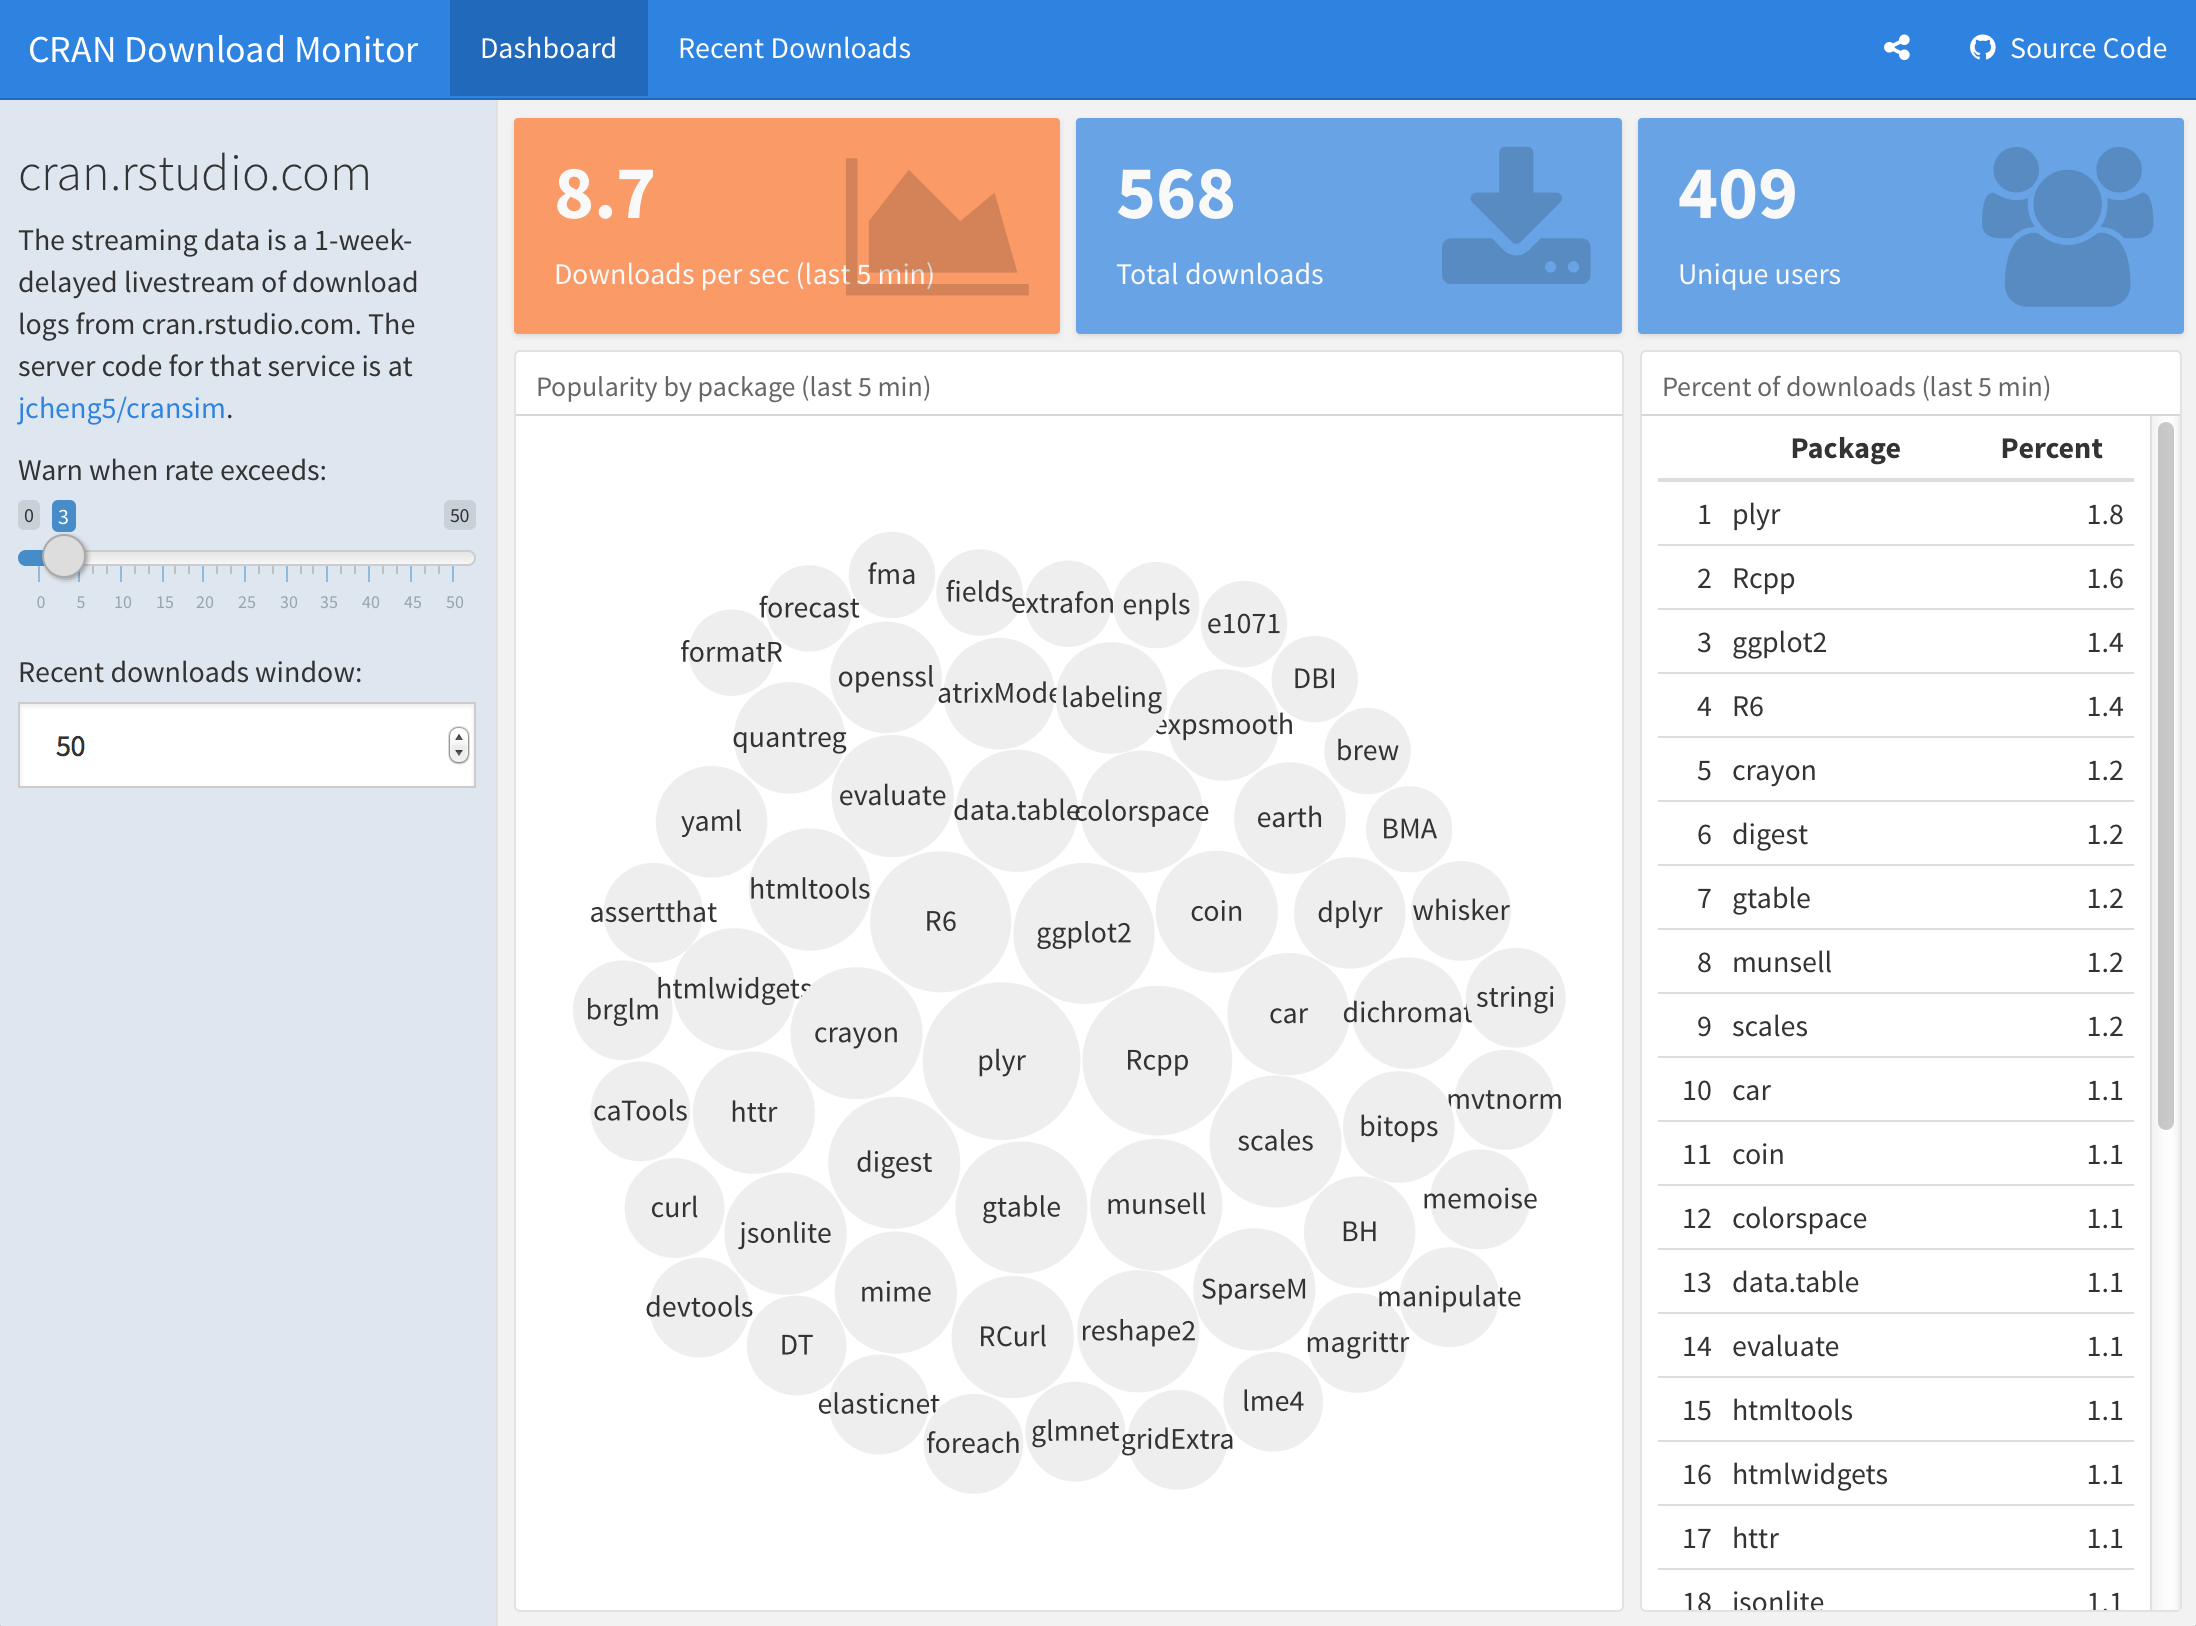
\includegraphics[width=.75\linewidth]{dashboard_shiny_example.png}
\caption{Exemplo de um aplicativo feito em Shiny.}
\label{fig:shiny_example}
\end{figure}

Este pacote permite a construção tanto da interface de interatividade com o usuário (conceito chamado de \textit{Front-End}), quanto da parte interna de sua construção em que o usuário não tem acesso (conceito chamado de \textit{Back-End}). O \textit{Front-End} é desenvolvido  pelo arquivo denominado \textit{ui.R} (de \textit{User Interface}) e o \textit{Back-End} é feito no arquivo \textit{server.R}.

Para diversos exemplos de aplicativos interativos fazendo uso do Shiny, recomenda-se o leitor acessar a seguinte galeria: https://shiny.rstudio.com/gallery/\footnote{Acesso em 24/10/2017.}.

\subsection{\textit{User Interface} e \textit{Server}\label{sec:ui}}

Conforme já comentado, os arquivos de interface de usuário (ui.R) e de servidor (server.R) são necessários para a criação de aplicações. Para o aplicativo funcionar é necessário que os objetos criados entre eles possuam os mesmos nomes de identificação, pois o usuário receberá inputs do \textit{Front-End}, processará no \textit{Back-End}, e devolverá um \textit{output} que pode ser um gráfico, por exemplo.

Nos Códigos \ref{code:ui_generico} e \ref{code:server_generico} é possível ver a criação de um aplicativo simples em que o usuário pode alternar a quantidade de classes de um histograma gerado a partir de um vetor de dados de uma base de dados. O aplicativo gerado é ilustrado na Figura \ref{fig:shiny_example_generico}.

%eval=false é pra não 'rodar' o código internamente, echo=true' é pra mostrar o código
\begin{rcode}
\begin{Schunk}
\begin{Sinput}
> library(shiny)
> # Definindo o User Interface
> shinyUI(fluidPage(
+   
+   # Título do Aplicativo
+   titlePanel("Exemplo de Aplicação Genérico"),
+   
+   # Barra lateral com um slider para o número de classes de um histograma
+   sidebarLayout(
+     sidebarPanel(
+        sliderInput("classes",
+                    "Número de Classes:",
+                    min = 1,
+                    max = 50,
+                    value = 30)),
+     
+     # Mostrar o plot gerado da distribuição
+     mainPanel(plotOutput("distPlot"))))
+   )
\end{Sinput}
\end{Schunk}
\caption{Exemplo de criação de \textit{User Interface}}
\label{code:ui_generico}
\end{rcode}

No Código \ref{code:ui_generico} acima é possível ver que um objeto chamado \texttt{classes} é criado que representa um \textit{slider} que varia do valor 1 até 50, tendo como valor padrão 30. Além disso é possível notar que no painel principal (\texttt{mainPanel}) será apresentado um objeto chamado \texttt{distPlot}.

\begin{rcode}
\begin{Schunk}
\begin{Sinput}
> # Definindo a lógica do servidor para desenhar um histograma
> shinyServer(function(input, output) {
+    
+   output$distPlot <- renderPlot({
+     
+     # Gere as classes baseadas no número imputado no arquivo ui.R
+     x    <- faithful[, 2] 
+     bins <- seq(min(x), max(x), length.out = input$classes + 1)
+     
+     # Desenhe o histograma como número de classes
+     hist(x, breaks = bins, col = 'darkgray', border = 'white')
+     
+   })
+   
+ })
\end{Sinput}
\end{Schunk}
\caption{Exemplo de criação de servidor}
\label{code:server_generico}
\end{rcode}

O Código \ref{code:server_generico} cria um objeto chamado \texttt{distPlot} com uma função de renderização que faz uso do objeto \texttt{classes} através da chamada \texttt{input\$classes} e cria um histograma com um vetor de dados que representa a segunda coluna da base de dados \texttt{faithful} que representa o tempo de espera, em minutos, entre as erupções de um vulcão.

\begin{figure}[H]
\centering
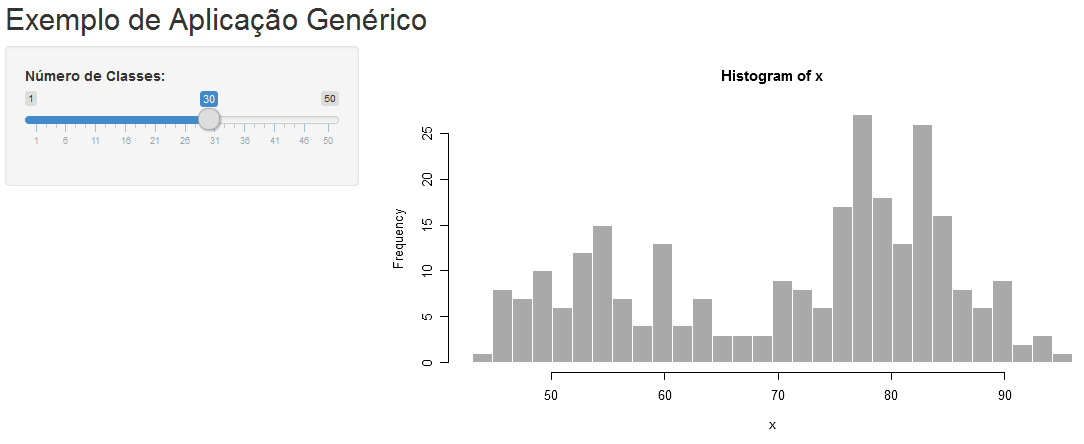
\includegraphics{shiny_generico.png}
\caption{Resultado de um aplicativo genérico construído}
\label{fig:shiny_example_generico}
\end{figure}

Na Figura \ref{fig:shiny_example_generico} é possível ver o resultado do exemplo de código criado. Neste aplicativo simples, o usuário pode alternar a quantidade de classes do histograma à esquerda com um \textit{slider} e ver o gráfico resultante à direita. Este exemplo ilustra como que os componentes entre o \textit{Front-End} e o \textit{Back-End} conversam entre si através de componentes comuns com nomes idênticos através do processamento do servidor e os componentes de entrada (\textit{input}) e saída (\textit{output}) do \textit{User Interface}.



\section{Interatividade gráfica: o pacote \texttt{htmlwidgets}\label{sec:htmlwidgets}}

Assim como a interatividade entre os componentes de entrada e saída do Shiny, a interatividade de um gráfico já criado é muito importante para uma análise visual mais acurada. A possibilidade de dar zoom, clicar em pontos específicos, remover pontos de um gráfico de dispersão, selecionar períodos de tempo específico em uma série temporal, investigar os metadados de uma observação, arrastar um mapa, aprofundar níveis de um gráfico, etc., são funcionalidades muito interessantes de se adicionar para instigar um usuário quanto ao dado que está sendo apresentado.

O \texttt{htmlwidgets}, já citado, é um pacote que permite criar outros pacotes de visualizações de dados interativas no R. Os pacotes \texttt{plotly} \cite{plotly}, \texttt{leaflet} \cite{leaflet}, \texttt{C3} \cite{c3}, \texttt{d3plus} \cite{d3plus} e \texttt{DT} \cite{DT} são os pacotes de interatividade que estão presentes no CrimeVis\footnote{Para ver a lista de todos os pacotes já realizados com o \texttt{htmlwidgets}, recomenda-se o acesso a lista em http://gallery.htmlwidgets.org/ - Acesso em 24/10/2017}.




\section{Construção do CrimeVis\label{sec:construcao_crimevis}}

Nesta seção apresenta-se com detalhes todos os componentes do CrimeVis a fim de apresentar de uma maneira intuitiva a dinâmica criminal municipal do RS. Foi de interesse usar a base de dados apresentada na Seção \ref{sec:base_tidy_crimevis}, que possui 44.664 valores (7.444 linhas e 6 colunas) compreendendo todos os municípios do estado, para todos os anos e para todos os tipos de crime de diversas maneiras visuais.

Vários tipos de gráficos interativos foram feitos: para acompanhar a dinâmica temporal da criminalidade, foram construídas visões de séries temporais; para verificar se existe relação criminal entre diferentes crimes nos município, criou-se gráficos de bolhas; para analisar a relação espacial do crime, mapas interativos foram criados; para analisar o grau de representatividade de cada município no estado, se criou gráficos de representação; e, por fim, para dispor todos os dados em uma tabela com filtros, uma tabela dinâmica, com toda a base, foi incluída com a possibilidade de realizar o download. Todas estas opções estão disponíveis no menu superior do aplicativo.

Excetuando o ambiente de Apresentação e de Download dos Dados do CrimeVis, o objetivo desta seção é apresentar cada uma destas diferentes visões criminais focando em como os códidos de \textit{Front-End} e \textit{Back-End} se relacionam. Ademais, se analisam os principais resultados encontrados em termos de ocorrências criminais no RS.

\subsection{Séries Temporais\label{sec:series_temporais}}

Uma das principais preocupações em segurança pública é avaliar o comportamento das taxas criminais ao longo do tempo. Avaliar se uma taxa está com uma tendência crescente ou decrescente em uma determinada região pode ser um sinal de que algo possa ser feito a fim de mitigar a taxa ou concentrar esforços em outras regiões.

Além disso, uma característica importante com relação às séries temporais é de que seja possível comparar diferentes tipos de crime no mesmo gráfico para cada região município ou estado. Por outro lado, é de interesse também que seja possível, dado um tipo de crime, comparar diferentes regiões. No primeiro caso, é possível analisar, por exemplo, que a evolução e a magnitude do roubo é bem diferente da do roubo de veículos em Porto Alegre, enquanto que no segundo caso, é possível verificar que as taxas de homicídio doloso do município de Alvorada são maiores do que as taxas de Porto Alegre.

Em termos de \textit{User Interface}, o Código \ref{code:ui_series} mostra como se pode criar uma aplicação em que o usuário pode selecionar um município (\texttt{selectInput}) e múltiplos crimes (\texttt{selectizeInput}). Além disso, como é de interesse avaliar tanto a criminalidade em termos de magnitude das ocorrências, quanto em termos de taxas por 100.000 habitantes inclui-se uma opção em que é possível optar pela visão entre a frequência absoluta de ocorrências ou a taxa (\texttt{radioButtons}). Por fim, apresentam-se os gráficos de séries temporais tanto a nível municipal, quanto estadual com o pacote \texttt{plotly} (\texttt{plotlyOutput}).

\begin{rcode}
\begin{Schunk}
\begin{Sinput}
> tabPanel("Compara Crimes",
+ sidebarLayout(
+ sidebarPanel(
+   selectInput('cidade_compara_crime', 'Cidade a ser escolhida', 
+           as.character(unique(base_crime$Mun)),
+           selected = "Porto Alegre"),
+   
+   selectizeInput('crimes_compara_crimes', 'Escolha até 5 crimes', 
+           as.character(unique(base_crime$Crime)),
+           selected = c("Homicídio Doloso"),
+           options = list(maxItems = 5,
+                        placeholder = 'Selecione uma lista de crimes...')),
+   
+   radioButtons("tipo_dado_compara_crime", "Tipo de Informação:",
+            c("Número de Ocorrências" = "ocorre_radio_compara_crime",
+              "Taxa por 100.000" = "taxa_radio_compara_crime"))),
+ 
+ # Mostrar o gráfico resultante
+ mainPanel(
+   tabsetPanel(type = "tabs", 
+             tabPanel("Municípios", plotlyOutput("ts_compara_crime_cidades")), 
+             tabPanel("Estado", plotlyOutput("ts_compara_crime_rs"))))))
\end{Sinput}
\end{Schunk}
\caption{User Interface de séries temporais}
\label{code:ui_series}
\end{rcode}

Na parte do servidor, são necessários três passos: 1) receber as entradas de municípios, crimes e tipo de informação; 2) manipular os dados e processar o gráfico; e 3) devolver a saída. O Código \ref{code:server_series} mostra, de uma maneira resumida, qual a chamada que deve ser feita para construir um gráfico de séries temporais no CrimeVis\footnote{Com relação à manipulação de dados, optou-se por suprimir o código devido ao seu tamanho. No entanto, neste momento o conceito de \textit{tidy data} é fundamental, tendo em vista duas características. Para a taxa criminal é necessário criar uma nova coluna com a função \textit{mutate} da seguinte forma: \texttt{mutate(Taxa = round(Qtd/Populacao*100000,2))} e, para criação de gráficos para múltiplos municípios, basta passar o argumento \texttt{color = \~{}Crime}. Estas duas facilidades só é possível graças à estrutura concisa construída e discutida na Seção \ref{sec:base_tidy_crimevis}.}.


\begin{rcode}
\begin{Schunk}
\begin{Sinput}
> output$ts_compara_cidades <- renderPlotly({
+   
+   # Manipulação da base suprimida
+ 
+   plot_ly(base_manipulada, x = ~Ano, y = ~Variavel, type = 'scatter', 
+           mode = 'lines', color = ~Crime, hoverinfo="text",
+           text = ~paste0(Crime, "<br>", nome, 
+                          Variavel, "<br>","Ano: ", Ano)) %>%
+     layout(title = cidade, yaxis = y_attr)
+ })
\end{Sinput}
\end{Schunk}
\caption{Servidor para as séries temporais}
\label{code:server_series}
\end{rcode}

Observe que esta visualização permite que se analise múltiplos tipos de crime para uma determinada região. No entanto, analogamente, é possível fixar um crime específico e comparar unidades geográficas. Os códigos para o cálculo desta visualização são análogos e não serão apresentados. Os resultados das Séries Temporais gerados pelo CrimeVis podem ser verificados na Figura \ref{fig:ts_crimevis}.

\begin{figure}[H]
\begin{subfigure}{.55\textwidth}
  \centering
  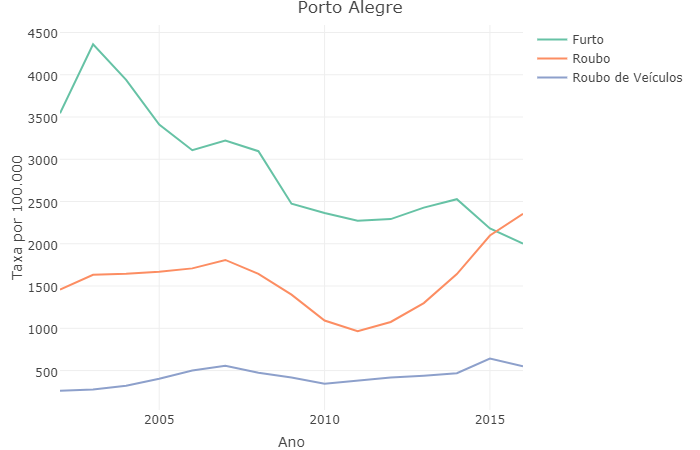
\includegraphics[width=.85\linewidth]{compara_crimes.png}
  \caption{Comparação de Crimes}
  \label{fig:comp_crime}
\end{subfigure}%
\begin{subfigure}{.55\textwidth}
  \centering
  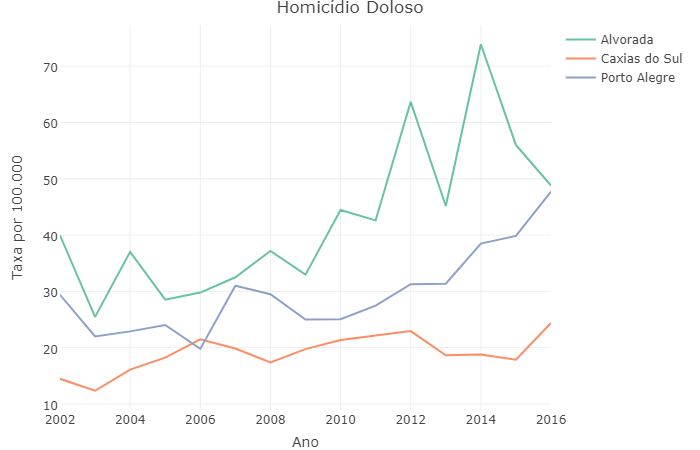
\includegraphics[width=.85\linewidth]{compara_cidades.png}
  \caption{Comparação de Cidades}
  \label{fig:comp_cidade}
\end{subfigure}
\caption{Séries Temporais geradas pelo CrimeVis}
\label{fig:ts_crimevis}
\end{figure}

Nesta figura é possível ver a evolução das ocorrências criminais sob diversos aspectos. Na subfigura \ref{fig:comp_crime} é possível ver a evolução das taxas por 100.000 habitantes do Furto, Roubo e Roubo de Veículos em Porto Alegre. Nitidamente, as taxas de furto são as maiores em comparação com os outros crimes, com exceção do ano de 2016 em que o Roubo ultrapassa o seu valor. Por outro lado, a subfigura \ref{fig:comp_cidade} mostra os índices de homicídio doloso em três municípios gaúchos: Porto Alegre, Alvorada e Caxias do Sul. Alvorada configura o município com os maiores índices de homicídios apresentando um valor de 48,8 em 2016.

\subsection{Relação entre crimes\label{sec:relacao_crimes}}

Muitas vezes é importante saber as inter-relações criminais em uma determinada região. Por exemplo, será que existem crimes que se relacionam entre si? Será que uma região que tem altas taxas de homicídio também tem altas taxas de roubo?  Alguns estudos na literatura, como \co{beato2001conglomerados} e \co{menezes2017relaccoes}, argumentam que existe uma relação positiva entre tráfico de entorpecentes e taxas de homicídios. Nesse sentido, é possível que isso possa ser investigado no CrimeVis.

Uma possibilidade de visualizar estas relações entre diferentes tipos de crimes para um determinado ano é um gráfico de dispersão que relaciona duas variáveis em dois eixos. No entanto, uma terceira informação pode ser incorporada na visualização que poderia dar a ideia do tamanho (representatividade) de uma determinada cidade (ponto no gráfico). Sendo assim, no CrimeVis, o gráfico que apresenta a relação criminal é um gráfico de bolhas (\textit{Bubble Plot}), que é um gráfico de dispersão com os tamanhos dos círculos proporcionais a uma variável numérica. No caso, a variável numérica usada é a população do município. 

O Código \ref{code:ui_relacao} ilustra quais são as principais entradas para a construção do gráfico de bolhas, que são os crimes para cada eixo (Homicídio Doloso e Roubo por padrão) e um seletor de população (\texttt{sliderInput}). O seletor de população é útil quando se deseja avaliar apenas um conjunto de municípios filtrando a base para apenas uma amplitude populacional específica. Por exemplo, pode ser de interesse avaliar apenas os municípios acima de 30.000 habitantes.

Além disso, um dos interesses foi adicionar uma funcionalidade de agrupamento de municípios com o método K-Means \cite{forgy1965cluster}. Estes agrupamentos mostram o grau de similaridade entre as diferentes medidas de criminalidade, considerando as suas distâncias entre os valores das variáveis de interesse. Em linhas gerais, o método agrupa municípios que estão mais próximos entre si no gráfico de bolhas. Em termos visuais no CrimeVis, cada grupo será ilustrado com uma cor na bolha.

\begin{rcode}
\begin{Schunk}
\begin{Sinput}
> sidebarPanel(
+ sliderInput('ano_disp', 'Ano a ser escolhido', 
+          min = min(base_crime$Ano), max = max(base_crime$Ano),
+          value = max(base_crime$Ano), step=1,
+          animate = animationOptions(interval = 1750, loop = TRUE), sep=""),
+ 
+ sliderInput('dispersao_mun_pop_control', "População:",
+          min = 0, max = 1500000, value = range(c(0, 1500000)), step = 2500),
+ 
+ selectInput('crimex', 'Selecione o crime do eixo horizontal', 
+          as.character(unique(base_crime$Crime)),
+          selected = "Homicídio Doloso"),
+                
+ selectInput('crimey', 'Selecione o crime do eixo vertical', 
+          as.character(unique(base_crime$Crime)),
+          selected = "Roubo"),
+ 
+ numericInput("n_grupos_kmeans", "Número de Grupos:", 3, min = 2, max = 496))
> mainPanel(plotlyOutput("dispersao"))
\end{Sinput}
\end{Schunk}
\caption{User Interface para a relação entre crimes}
\label{code:ui_relacao}
\end{rcode}


Em termos de código do servidor da relação entre crimes, o Código \ref{code:server_relacao} e a base transformadada da Tabela \ref{out:base_bolha} (\texttt{base\_bolha}) abaixo apresentam a maneira como é construído o gráfico de bolhas com todos os seus componentes. É possível notar como as quatro medidas estão sendo utilizadas dentro da função \texttt{plot\_ly}: a variável do eixo horizontal (\texttt{X}), a variável do eixo vertical (\texttt{Y}), a variável de tamanho dos círculos (\texttt{Pop}) e a variável de coloração dos círculos (\texttt{Grupos}). Todas as quatro medidas estão reunidas em uma única chamada de função, de uma única tabela e em um único gráfico gozando integralmente das propriedades de \textit{tidy data} e da gramática de gráficos discutidas anteriormente.



\begin{rcode}
\begin{Schunk}
\begin{Sinput}
> plot_ly(base_bolha, x = ~X, y = ~Y, size=~base_bolha$Pop, color = ~Grupos,
+         type = 'scatter', mode = 'markers', hoverinfo="text",
+         text = paste("", base_bolha$Grupo, "<br>",
+                      muni, "<br>", 
+                      "População :", base_bolha$Pop, "<br>",
+                      crime_x, ":", base_bolha$X, "<br>",
+                      crime_y, ":", base_bolha$Y),
+         marker = list(opacity = 0.5, sizemode = 'diameter'), 
+         showlegend = FALSE)
\end{Sinput}
\end{Schunk}
\caption{Servidor para a relação entre crimes}
\label{code:server_relacao}
\end{rcode}


\begin{routput}[H]
\begin{Schunk}
\begin{Soutput}
# A tibble: 497 × 5
       X       Y   Pop  Grupos       muni
   <dbl>   <dbl> <int>  <fctr>      <chr>
1  21.76 1305.77  4595 Grupo 2     Aceguá
2  50.77 1040.87  3939 Grupo 5 Água Santa
3  29.89 1028.09 16730 Grupo 5      Agudo
4  40.21  777.38  7461 Grupo 5  Ajuricaba
5  15.13 1437.22  6610 Grupo 2    Alecrim
6 201.67 1068.18 76860 Grupo 5   Alegrete
# ... with 491 more rows
\end{Soutput}
\end{Schunk}
\caption{Base de Dados \textit{tidy} da relação entre crimes}
\label{out:base_bolha}
\end{routput}

Um exemplo de resultado de uma visualização do gráfico de bolhas pode ser conferido na Figura \ref{fig:relacao_screen} em que são relacionadas as taxas Furto no eixo vertical e Homicídio Doloso no eixo horizontal para o ano de 2014. Observe que os tamanhos dos círculos são proporcionais aos tamanhos dos municípios e, por isto, Porto Alegre é a cidade representada pelo maior círculo presente no meio do gráfico. O município de Alvorada que possui uma considerável população de, 211.097 habitantes, está destacado no canto inferior direito.

Adicionalmente, as cores dos círculos representam a criação de seis grupos gerados pelo método K-Means. Estão destacados os municípios pertencentes ao Grupo 4 que são compostos basicamente por municípios pertencentes ao litoral norte do RS como Xangri-lá, Arroio do Sal, Imbé, Cidreira, Tramanadaí, Capão da Canoa e Balneário Pinhal. Estes municípios litorâneos apresentam altas taxas de Furto como já discutido em \co{cortes2016tdfee}.

\begin{figure}[H]
\centering
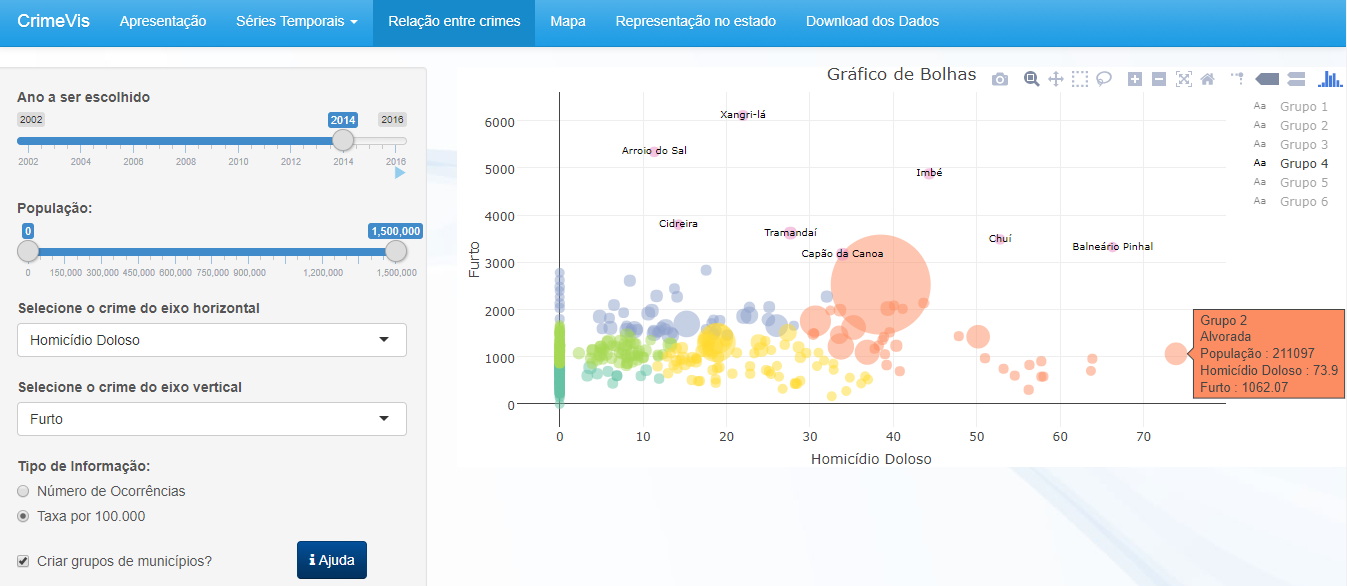
\includegraphics[width=.75\linewidth]{screenshot_relacao2.png}
\caption{Exemplo de relação entre Homicídio Doloso e Furto com destaque em um grupo de municípios}
\label{fig:relacao_screen}
\end{figure}


\subsection{Mapas\label{sec:mapa}}

A representação espacial sempre foi de grande interesse na investigação visual de dados. Dentro do contexto do CrimeVis, os mapas construídos se constituem nas localizações das ocorrências criminais ao longo dos anos nos municípios do RS, ressaltados através de um gradiente de cores. Neste gradiente de cores, é possível avaliar quais são as regiões com menores índices criminais (áreas cinzas) e maiores índices (áreas vermelhas).

O recente pacote \texttt{leaflet} permite que o usuário faça rapidamente, e em poucas linhas de código, gráficos interativos em que é possível: dar/retirar zoom; clicar em regiões específicas para visualizar mais informações; arrastar o mapa; criar gradientes (ou classes) de cores; mudar o fundo/tipo de mapa, etc\footnote{O \texttt{leaflet} também é utilizado por grandes empresas como Facebook, Pinterest, GitHub, Foursquare, The Washington Post, etc.}. A grande facilidade de seu uso, atrelado ao fato de gozar também das propriedades da gramática de gráficos aplicada para mapas, faz com que este pacote seja amplamente difundido.

Uma funcionalidade de interesse também na avaliação criminal é saber se a criminalidade de uma região afeta uma região próxima. Em outras palavras, é necessário saber se existe um \textit{efeito espacial} na criminalidade entre os municípios gaúchos. A fim de contemplar esta análise, se desenvolveu no CrimeVis a possibilidade de calcular também a autocorrelação espacial através do índice I de Moran \cite{moran1950biometrika}. Este índice, condicionado a uma estrutura espacial, varia de -1 a 1 indicando se municípios vizinhos possuem alto grau de concordância criminal (valor próximo de 1) ou alto grau de discordância criminal (valor próximo de -1)\footnote{Os códigos referentes ao cálculo do I de Moran não serão apresentados aqui.}.

Em termos de códigos, é necessário que o usuário opte pelo ano, tipo de crime e o tipo de informação (número de ocorrências ou taxa por 100.000 habitantes) para visualizar o mapa criminal desejado. A entrada dos valores do \textit{User Interface} é muito similar ao que já foi apresentado até o momento e, por este motivo, não será apresentado.

Na parte do servidor, o Código \ref{code:server_mapa} ilustra como o mapa é construído para uma taxa criminal de um ano específico. Primeiramente, se filtra a base de dados (\texttt{filter}) de acordo com o ano e o tipo de crime escolhido criando uma base auxiliar para porteriormente combinar com um arquivo de mapas (\texttt{mapa\_rs}). Posteriormente, cria-se um gradiente de cores e chama-se a função \texttt{leaflet} que novamente goza das propriedades de \textit{tidy data} e da gramática de gráficos, neste caso, aplicada a contrução de mapas uma vez que diversas camadas são adicionadas.

\begin{rcode}
\begin{Schunk}
\begin{Sinput}
> output$mapa_final <- renderLeaflet({
+ df_aux_pre <- filter(base_crime, 
+                      Ano == input$ano_mapa & 
+                      Crime == input$crime_mapa)
+ df_aux <- mutate(df_aux_pre, Taxa = Qtd / Populacao * 100000)
+ df_mapa <- merge(mapa_rs, df_aux, 
+                  by.x = "GEOCODIG_M", 
+                  by.y="CodIBGE", all.x = FALSE)
+ 
+ gradiente = colorNumeric(c("lightgrey", "yellow", "orange", "Red"), 
+                          domain = df_mapa$Taxa)
+ 
+ leaflet(data = df_mapa) %>% 
+     addTiles('http://{s}.tile.openstreetmap.org/{z}/{x}/{y}.png') %>%
+     addPolygons(weight = 0.5, fillColor = ~gradiente(df_mapa$Taxa), 
+                 color = "grey", fillOpacity = 0.5, 
+                 smoothFactor = 0.25,
+                 popup = paste0(df_mapa$Nome_Munic, "<br>",
+                                "Pop.: ", df_mapa$Populacao, "<br>",
+                                "Qtd.: ", df_mapa$Qtd, "<br>",
+                                "Tx.: ", round(df_mapa$Taxa,2))) %>% 
+     addLegend(position = "bottomright", pal = gradiente, values = ~Taxa)
+ })
\end{Sinput}
\end{Schunk}
\caption{Servidor para o mapa}
\label{code:server_mapa}
\end{rcode}

Em termos de resultados das taxas, a Figura \ref{fig:mapa_crimevis} apresenta dois exemplos que são interessantes espacialmente para o RS em 2016: roubo de veículos e furtos. No caso do roubo de veículos, percebe-se que as maiores taxas estão concentradas basicamente na região metropolitana de Porto Alegre. Uma das alegações dos agentes de segurança pública é a de que os carros que são roubados na capital muitas vezes são levados para desmanche em municípios vizinhos, como Alvorada ou Viamão. Sob esta hipótese, existe um forte componente de efeito espacial neste tipo de crime que é confirmado com a medida de autocorrelação de 0,537 pontos supondo uma estrutura de vizinhos que compartilham borda. Este mapa conjuntamente com a medida de autocorrelação no CrimeVis está na subfigura \ref{fig:mapa_roub} 

\begin{figure}[H]
\begin{subfigure}{.55\textwidth}
  \centering
  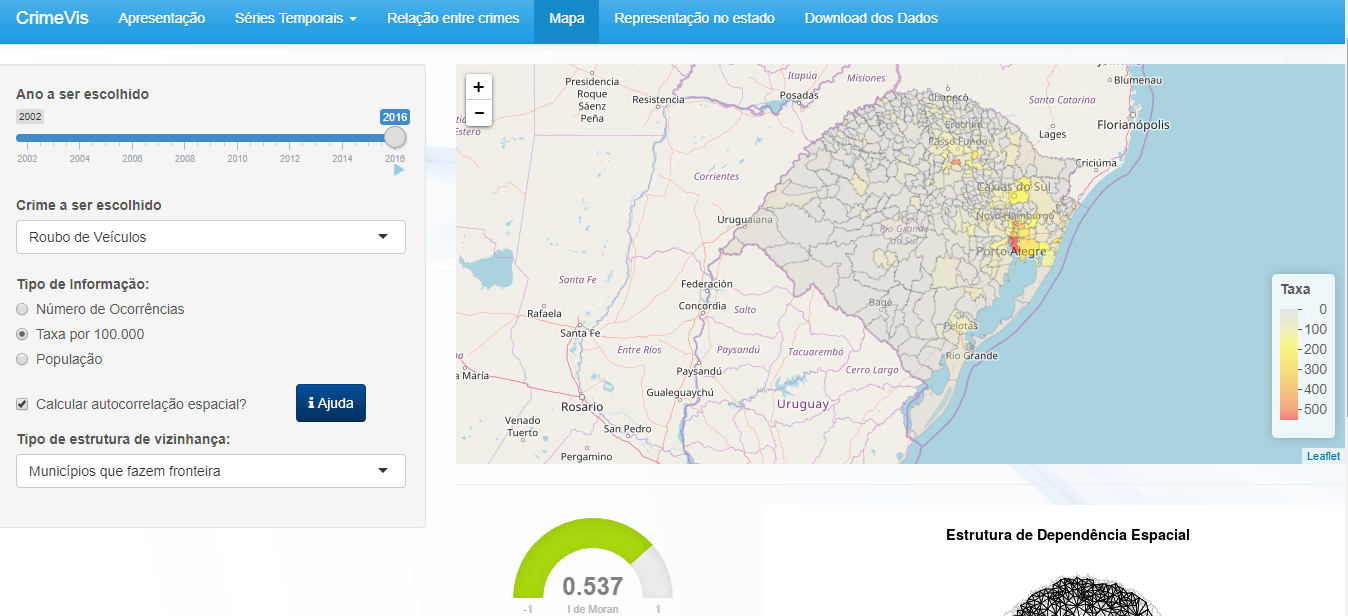
\includegraphics[width=.85\linewidth]{mapa_roubo_veic.png}
  \caption{Mapa do Roubo de Veículos no CrimeVis}
  \label{fig:mapa_roub}
\end{subfigure}%
\begin{subfigure}{.55\textwidth}
  \centering
  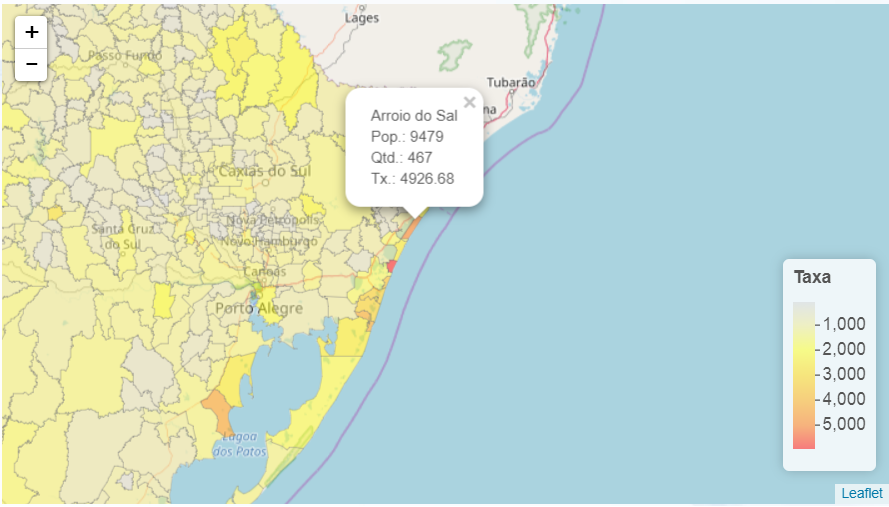
\includegraphics[width=.85\linewidth]{mapa_destaque_furto.png}
  \caption{Destaque no mapa de Furto no litoral norte}
  \label{fig:mapa_furto}
\end{subfigure}
\caption{Mapas gerados pelo CrimeVis}
\label{fig:mapa_crimevis}
\end{figure}

Por fim, a subfigura \ref{fig:mapa_furto} ressalta as taxas de furto do estado dando destaque para os municípios que possuem os maiores valores, que são os pertencentes ao litoral norte. Como visto anteriormente na Seção \ref{sec:relacao_crimes}, estes municípios podem ser vistos como pertencentes a um grupo similar devido à altas taxas de furto. Isto se revela ressaltado em cores mais alaranjadas e avermelhadas neste mapa, que mostra estes dados dando um zoom nesta região e tendo como destaque o município de Arroio do Sal.



\subsection{Representação no estado\label{sec:representacao}}

O último tipo de visualização de dados presente no CrimeVis é a de Representação no estado, ilustrada através de um gráfico de \textit{treemap} (também chamado de mapa de árvore). Este tipo de gráfico ilustra a representação de unidade de medida (ou nível de uma variável) no contexto total através da combinação de subretângulos proporcionais. Em outras palavras, a área de cada retângulo é proporcional à soma total de uma variável numérica. No CrimeVis, utiliza-se o pacote \texttt{d3plus} para a construção do treemap. Esta ferramenta é construída tendo como base a biblioteca javascript \textit{d3.js} \cite{teller2013data} e que possui diversos outros tipos de visualização. Neste tipo de gráfico é possível ver quais são os municípios que possuem as maiores participações de ocorrências criminais no RS, visualizado em termos de proporcionalidade dos retângulos construídos.

Condicionado a um ano específico e um tipo de crime específico, o Código \ref{code:server_treemap} do servidor mostra como é a construção de um \textit{treemap} no R usando o \texttt{d3plus}.

\begin{rcode}
\begin{Schunk}
\begin{Sinput}
>   output$tree_map <- renderD3plus({
+     df_aux <- filter(base_crime, 
+                      Ano == input$ano_tree & 
+                      Crime == input$crime_tree) %>% 
+               select(Mun, Qtd)
+     d3plus(df_aux, "tree")
+   })
\end{Sinput}
\end{Schunk}
\caption{Servidor para o \textit{treemap}}
\label{code:server_treemap}
\end{rcode}

Um exemplo de resultado pode ser conferido na Figura \ref{fig:treemap_ex} onde, novamente, a ocorrência de roubo de veículos é evidenciada. É possível notar que o retângulo de Porto Alegre representa praticamente a metade da área de todo o gráfico. De fato, a capital apresentou cerca de 46\% de todas as ocorrências criminais do estado em 2016 e, por este motivo, ocupa uma área significativa neste gráfico.

\begin{figure}[H]
\centering
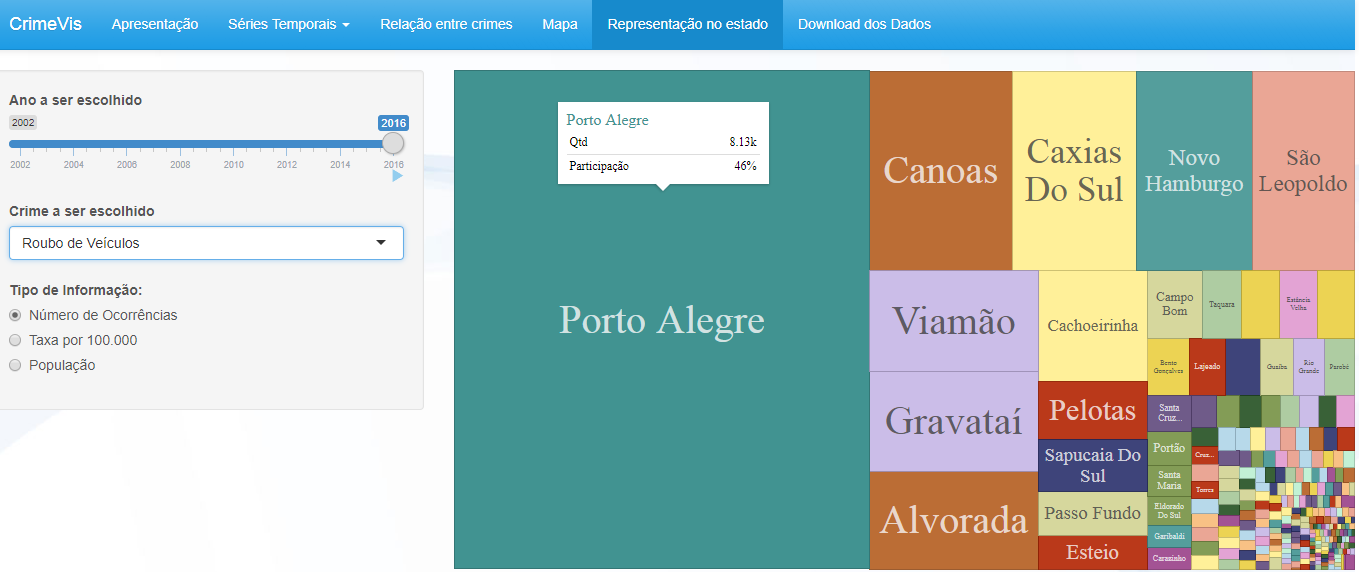
\includegraphics[width=.75\linewidth]{exemplo_treemap.png}
\caption{Exemplo de \textit{treemap} de Roubo de Veículos em 2016}
\label{fig:treemap_ex}
\end{figure}

\section{Considerações Finais\label{sec:consideracoes_finais}}

Este trabalho apresentou detalhadamente os componentes e a construção do aplicativo de visualização de dados criminais do Rio Grande do Sul (RS) \textbf{CrimeVis}, usando a tecnologia \textit{Shiny}. Com a motivação de que a análise visual de dados desempenha um papel fundamental na investigação de padrões que, às vezes, podem passar despercebidos, o CrimeVis permite que o usuário tenha uma noção panorâmica da dinâmica criminal do RS sob diferentes óticas de visualização.

Além das visualizações apresentadas, este trabalho avança na literatura na medida em que ele consolida diversas estatísticas históricas e de diferentes tipos de crimes em uma única base de dados, apresentando-as de maneira amigável, intuitiva e dinâmica para a sociedade. Ademais, ele discute conceitos novos que surgiram no campo da análise de dados que se configuram como melhores práticas tanto na parte de manipulação de dados quanto de visualização através dos conceitos de \textit{tidy data} e da gramática de gráficos.

Em termos de benefícios para adoção de medidas para políticas públicas, foi visto que existe uma tendência crescente das taxas de homicídio doloso em algumas das principais cidades do estado como Porto Alegre, Caxias do Sul e Alvorada. Além disso, foram identificados agrupamentos espaciais municipais para crimes específicos. Foi identificada uma região de alta taxa de furtos no litoral norte e outra de alta taxa de roubos de veículos em municípios da região metropolitana. Tais resultados podem auxiliar na otimização de alocação de recursos e otimizar a eficiência policial a fim de mitigar o comportamento delinquencial.

Para trabalhos futuros, é de interesse aprofundar ainda mais o estudo da criminalidade no RS. Crimes intramunicipais a fim de identficar quais são as regiões mais perigosas em termos de bairros, ruas, horários, etc. seria de grande valia para a população e para os gestores públicos. No entanto, para isto, é necessário ter informações intra-urbanas.

Por fim, cabe ressaltar que, apesar de diversas ferramentas de visualização de dados já existirem, acredita-se que o CrimeVis é uma importante contribuição para qualificar o acesso às estatísticas públicas. Ele faz parte de um portal de visualização de dados, VisualizaFEE, e todo o seu código, base de dados, arquivos suplementares estão disponíveis gratuitamente em https://github.com/renanxcortes/VisualizaFEE/tree/master/crime.







\chapter{Cadeias de Markov Espaço-Temporais dos crimes no RS: análise e acoplamento no CrimeVis}

\section{Introdução\label{sec:Introducao_acoplamento}}

A atividade criminal é um fenômeno que pode depender tanto do espaço quanto do tempo. Diversos trabalhos analisaram o efeito espaço-temporal na criminalidade podendo-se citar \co{neema2012monitoring}, \co{rey2012exploratory}, \co{shiode2015space} e \co{newton2015crime}. Segundo \co{rey2012exploratory}, apesar do reconhecimento desta dependência temporal e espacial, até recentemente, estes componentes eram pouco utilizados devido à complexidade envolvida neste tipo de análise.

Modelos markovianos representam uma maneira simples de representar um fenômeno através de uma estrutura de dependência condicional \cite{rue2005gaussian}. Esta estrutura pode compreender tanto a dependência espacial quanto a temporal. A ideia por trás de modelos markovianos é de que o fenômeno  analisado depende somente de um sub conjunto dos dados, simplificando a abordagem e reduzindo a complexidade das estimações. A estrutura de dependência espacial pode ser dada via um grafo estruturado de vizinhanças espaciais e a estrutura temporal pode ser dada pela dependência de um ou mais períodos do passado.

Em termos de utilização de modelos de Markov na criminalidade, \co{stander1989markov} fizeram uso de dados longitudinais de homens delinquentes para verificar se eles ''migravam'' de um tipo de delito para outro ao longo do tempo. Neste estudo, foi verificado que o tipo de crime do passado ajuda a prever o tipo de crime do futuro devido ao baixo valor das probabilidades de transição, sugerindo que existe uma especialização no tipo de crime praticado. \co{rey2012exploratory}, usando dados da cidade de Mesa no Arizona, fazem uso de cadeias de Markov para prever a transição de um período inicial de uma região em que houve roubo (ou não) para verificar se as regiões apresentaram roubo (ou não) em um período final. Além disso, neste trabalho são estimadas também matrizes de transiçao markovianas espaço-temporais em que a vizinhança pode (ou não) afetar a presença de roubos no futuro de uma determinada região.

No presente trabalho, tendo em vista que o objeto de estudo é a transição de estado entre a presença/ausência de determinado crime de uma determinada região, é importante ressaltar qual é a unidade observacional estudada. A região de abrangência das análises será o nível municipal do Rio Grande do Sul (RS). Ou seja, será de interesse avaliar as transições dos municípios em relação aos crimes nos períodos determinados. Aplicar estas medidas para que, de certa maneira, predizer o comportamento probabilístico espaço-temporal do RS representa uma importante contribuição em termos de segurança pública para os agentes públicos. 

O CrimeVis\footnote{Disponível em http://visualiza.fee.tche.br/crime - Acesso em 10/11/2017.} \cite{renan2017crimevis} é uma recente plataforma de visualização de dados dos crimes do RS. Esta ferramenta apresenta os dados das ocorrências criminais anuais de diversas categorias de crimes de maneira interativa com séries temporais, gráficos de relação, mapas dinâmicos, \textit{treemaps}, etc. Este trabalho tem como objetivo, além de explorar as cadeias de Markov espaço-temporais criminais, discutir e apresentar a inclusão destas funcionalidades no CrimeVis.

De acordo com \co{rey2012exploratory} muitas técnicas são utilizadas para abordar a questão espaço-temporal como testes estatísticos epidemiológicos e modelos matemáticos sofisticados para tentar predizer o comportamento criminal através do espaço e do tempo. No entanto, muitos estudos se apegam a comparações visuais de mapas que identificam locais de maior criminalidade. Este esforço, no entanto, fornece medidas de resumo da criminalidade da área de estudo, mas não contempla a questão conjunta da evolução espaço-temporal. O presente trabalho se diferencia neste aspecto, uma vez que ele, além de incluir a questão visual através de mapas no CrimeVis, incorpora de maneira simples a questão da mudança espaço-temporal dos crimes no RS através de modelos de Markov.

\section{Metodologia\label{sec:metodologia_acoplamento}}

\subsection{Base de Dados\label{sec:base_de_dados_acoplamento}}

A base de dados utilizada neste artigo compreende as ocorrências anuais da Secretaria de Segurança Pública do RS (SSP-RS). Ela possui uma série histórica de 15 anos (variando de 2002 até 2016) para diversos tipos de ocorrências criminais e para todos os 496 municípios do estado\footnote{Para garantir a comparabilidade de toda a série histórica, o município de Pinto Bandeira, que foi emancipado somente em 2013, não foi incluído na análise.}. A base contempla crimes de Homicídio Doloso, Latrocínio, Roubo, Roubo de Veículos, Furto, Furto de Veículos, Delitos Relacionados à Armas e Munições, Delitos Relacionados a Corrupção, Posse de Entorpecentes, Tráfico de Entorpecentes, Extorsão, Extorsão Mediante Sequestro e Estelionato.

\subsection{Cadeias de Markov\label{sec:cadeias_acoplamento}}

Cadeias de Markov são um caso particular de um processo estocástico discreto. Formalmente, uma cadeia de Markov é uma sequência de variáveis aleatórias $X_1,X_2,X_3,...$ em que a distribuição de probabilidade condicional de uma dada variável depende somente de uma variável (ou de um subconjunto). Por exemplo:
\begin{equation}
P(X_{t+1} = x \mid X_0,X_1,...,X_t) = P(X_{t+1} = x \mid X_t)
\label{eq:prob_cond_generica}
\end{equation}
onde $x$ é uma possível realização das variáveis aleatórias.

Neste trabalho, a variável sob análise é a presença ou ausência de alguma ocorrência criminal em um determinado espaço (município) e em um determinado tempo (ano). Em termos temporais, para a construção das matrizes de transição de estados, este artigo assume que o estado de apresentar ou não um evento criminal de um município, depende da presença ou ausência de crimes num período anterior ou inicial ($t=0$). Para maiores informações sobre cadeias de Markov, é possível consultar \co{norris1998markov}.

\subsection{Matrizes de Transição Temporais\label{sec:temporais_acoplamento}}


As matrizes de transição temporal representam as probabilidades de transição de um estado para o outro. Neste caso, o estado de interesse é uma variável \textit{dummy} assumindo valor um, se houve pelo menos uma ocorrência criminal no município, e zero, caso contrário.

Seguindo \co{rey2012exploratory}, a dependência markoviana é uma cadeia de Markov discreta de primeira ordem em que $X(t) \mid t \in T$ tal que, para qualquer $t_0 < t_1 < ... < t_T$, a distribuição cumulativa funcional de $X(t_l)$ depende somente de $X(t_{l-1})$. Se $X(t)$ é discreto e que pode assumir $k$ diferentes valores, então ele é uma cadeia homogênea no tempo se:
\begin{small}
\begin{equation}
P[ X(t_l)=j \mid  X(t_{l-1})=i, X(t_{l-2})=j,...,X(t_{0})=i]=P[ X(t_l)=j \mid  X(t_{l-1})=i]=p_{i,j} \ \forall i,j
\label{eq:prob_cond_time_invariant}
\end{equation}
\end{small}
e $p_{i,j}$ satisfazem as seguintes condições:
% "\" é um símbolo para adicionar um espaço em branco no meio de uma fórmula no latex
% O "[]" no "\item[]" retira os pontos na descrição dos itens.

\begin{align*}
0 \leq p_{i,j} \leq 1 \\
\sum _jp_{i,j}=1 \ \forall i
\end{align*}
onde $p_{i,j}$ é a probabilidade de uma célula da matriz que estava no estado $i$ no período inicial passe para o estado $j$ no período final. Neste caso, existem $k=2$ estados possíveis: não houve nenhuma ocorrência de crime ($X = 0$) e houve alguma ocorrência de crime ($X = 1$).

O estimador de máxima verossimilhança destas probabilidades de transição são dadas por:
\begin{equation}
\widehat{p_{i,j}}=\frac{f_{i,j}}{\sum _jf_{i,j}}
\end{equation}
onde $f_{i,j}$ é a frequência de transições do estado $i$ no período inicial para o estado $j$ no período final. Um exemplo desta matriz de probabilidades de transição é apresentado na Tabela \ref{tab:matriz_transicao_temporal_generica}.

% Fui editando este genérico:
%\begin{table}[h]
%\centering
%        \begin{tabular}{lll}
%            \hline
%            \multirow{4}{*}{XXX} & \multicolumn{1}{l}{XXX} & \multicolumn{1}{l}{XXX} \\\cline{2-3} % As colunas 2 e 3 terão uma linha abaixo
%                                 & \multicolumn{1}{l}{XXX} & \multicolumn{1}{l}{XXX} \\\cline{2-3}
%                                 & \multicolumn{1}{l}{XXX} & \multicolumn{1}{l}{XXX} \\\cline{2-3}
%                                 & \multicolumn{1}{l}{XXX} & \multicolumn{1}{l}{XXX} \\\hline
%            \ttfamily xxx & \ttfamily xxx & \ttfamily xxx \\                \hline
%        \end{tabular}
%    \caption{xxx}
%    \label{tab:xxx}
%\end{table}

\begin{table}[H]
\centering
        \begin{tabular}{ccc}
            \hline
            \multirow{2}{*}{Estado Inicial ($t_0$)} & \multicolumn{2}{c}{Estado Final ($t_1$)}  \\\cline{2-3} 
                                     & \multicolumn{1}{l}{Sem Crime} & \multicolumn{1}{l}{Com Crime} \\\hline
            {Sem Crime} & {$p_{1,1}$} & {$p_{1,2}$} \\                \hline
            {Com Crime} & {$p_{2,1}$} & {$p_{2,2}$} \\                \hline
        \end{tabular}
    \caption{Exemplo de Matriz de Transição Temporal}
    \label{tab:matriz_transicao_temporal_generica}
\end{table}

Nesta tabela, a probabilidade de um município que não apresentou crime no período inicial passar a apresentar no período final é $p_{1,2}$. Por outro lado, a probabilidade de um município, que apresentou crime no período inicial, passar a não apresentar no período final é $p_{2,1}$. As probabilidades da região não trocar de estado são $p_{1,1}$ (ausência de crime) e $p_{2,2}$ (presença de crime).
%- explicar oque é ergódico

\subsection{Matrizes de Transição Espaço-Temporais\label{sec:espaco_temporais_acoplamento}}

Uma das hipóteses que as matrizes temporais fazem é a homogeneidade espacial. A Tabela \ref{tab:matriz_transicao_temporal_generica} assume que todos os municípios, independente da sua localização e da sua estrutura de vizinhança, estão sujeitos à mesma estrutura de probabilidades de transição. No entanto, muitas vezes é necessário incorporar também a estrutura espacial na evolução da criminalidade, uma vez que este componente pode afetar a dinâmica das ocorrências, pois é razoável supor que os crimes não ocorrem de maneira espacialmente aleatória. Neste contexto, \co{rey2001spatial} introduz a extensão das matrizes de transição markovianas que permitem uma análise mais acurada das dimensões geográficas da dinâmica de transição.

Esta abordagem leva em consideração a vizinhança dos municípios\footnote{A vizinhança estabelecida é a de contiguidade de primeira ordem em que um município é considerado vizinho de outro se eles compartilham borda ou um ponto em comum. Este tipo de estrutura de vizinhança também é chamada de \textit{queen}.} no período inicial da análise. Sendo assim, a amostra é dividida em dois estratos de municípios: municípios que tiveram pelo menos um vizinho que teve crime no período e inicial e municípios em que todos os vizinhos não apresentaram crimes no período inicial.

A Tabela \ref{tab:matriz_transicao_espaco_temporal_generica} apresenta a matriz markoviana espaço-temporal da criminalidade utilizada. As probabilidades associadas apresentam um novo subíndice onde $sc$ significa \textit{Sem Crime} na vizinhança no período inicial e $cc$ significa \textit{Com Crime} na vizinhança no período inicial.



%- As matrizes de transição temporais possuem uma limitação

\begin{table}[H]
\centering
        \begin{tabular}{cccc}
            \hline
            \multirow{2}{*}{Vizinhança ($t_0$)} & \multirow{2}{*}{Estado Inicial ($t_0$)} & \multicolumn{2}{c}{Estado Final ($t_1$)}  \\\cline{3-4} % As colunas 3 e 4 terão uma linha abaixo
                                        & & \multicolumn{1}{l}{Sem Crime} & \multicolumn{1}{l}{Com Crime} \\\hline
            \multirow{2}{*}{Sem Crime} & {Sem Crime} & {$p_{sc,1,1}$} & {$p_{sc,1,2}$} \\
                                       & {Com Crime} & {$p_{sc,2,1}$} & {$p_{sc,2,2}$} \\\hline
            \multirow{2}{*}{Com Crime} & {Sem Crime} & {$p_{cc,1,1}$} & {$p_{cc,1,2}$} \\
                                       & {Com Crime} & {$p_{cc,2,1}$} & {$p_{cc,2,2}$} \\\hline
        \end{tabular}
    \caption{Exemplo de Matriz de Transição Espaço-Temporal}
    \label{tab:matriz_transicao_espaco_temporal_generica}
\end{table}

Com esta extensão, é possível verificar as diferentes matrizes de transição de probabilidades para cada um dos estratos. Além disso, possibilita uma investigação do efeito espaço-temporal conjunto dos crimes.


\subsection{Razões de Chances Temporais e Espaço-Temporais\label{sec:odds_acoplamento}}

Sob a hipótese de que não existe efeito espacial, é possível calcular as razões de chance da evolução espacial através do quociente entre as probabilidades de transição. Na Tabela \ref{tab:matriz_transicao_temporal_generica} é possível calcular a chance de uma célula que não apresentou crime no período inicial, venha a apresentar crime no período final ($\Pi_{1,2}$). De maneira similar, pode-se calcular a chance de uma célula transitar para a presença de crime no período final em relação ao fato de que ela não apresentou crime no período inicial ($\Pi_{2,1}$). Por fim, existem duas medidas de chance de uma célula permanecer no mesmo estado, seja sem crime ($\Pi_{1,1}$) ou com crime ($\Pi_{2,2}$). Estas razões de chance são calculadas conforme a seguir:
\begin{equation}
\Pi_{1,2}=\frac{p_{1,2}}{p_{1,1}},\ \ \Pi_{2,1}=\frac{p_{2,1}}{p_{2,2}}, \ \ \Pi_{1,1}=\frac{p_{1,1}}{p_{1,2}}, \ \ \Pi_{2,2}=\frac{p_{2,2}}{p_{2,1}}.
\label{eq:odds_temporal}
\end{equation}

Além disso, a fim de incorporar também o contexto espacial nestas medidas, é possível calcular as razões de chance espaço-temporais. Seja $\Pi(CC)$ as razões de chance temporais do estrato que ocorreu crime na vizinhança e $\Pi(SC)$ as razões de chance temporais do estrato que não ocorreu crime na vizinhança, analisando a Tabela \ref{tab:matriz_transicao_espaco_temporal_generica}, as razões de chance espaço-temporais são dadas pelas seguintes fórmulas:
\begin{align}
\begin{split} % Este ambiente permite um número único para todas equações (talvez o aligned funcionasse também)
\theta_{1,2}=\frac{\Pi(CC)_{1,2}}{\Pi(SC)_{1,2}}=\frac{\frac{p_{cc,1,2}}{p_{cc,1,1}}}{\frac{p_{sc,1,2}}{p_{sc,1,1}}}, \ \theta_{2,1}=\frac{\Pi(CC)_{2,1}}{\Pi(SC)_{2,1}}=\frac{\frac{p_{cc,2,1}}{p_{cc,2,2}}}{\frac{p_{sc,2,1}}{p_{sc,2,2}}}, \\ \\ \theta_{1,1}=\frac{\Pi(CC)_{1,1}}{\Pi(SC)_{1,1}}=\frac{\frac{p_{cc,1,1}}{p_{cc,1,2}}}{\frac{p_{sc,1,1}}{p_{sc,1,2}}}, \ \theta_{2,2}=\frac{\Pi(CC)_{2,2}}{\Pi(SC)_{2,2}}=\frac{\frac{p_{cc,2,2}}{p_{cc,2,1}}}{\frac{p_{sc,2,2}}{p_{sc,2,1}}}
\label{eq:odds_ratio_espaco_temporal}
\end{split}
\end{align}

Observa-se que as razões de chances dos $\theta$'s são quocientes das razões de chance temporais que representam o \textbf{efeito de ter vizinhança criminosa na transição temporal}. Por exemplo, a chance de uma célula que teve vizinhança criminosa no período inicial de transitar dos estados $Sem \ Crime \rightarrow Com \ Crime$ é $\theta_{1,2}$ vezes se elas não tivessem tido crimes na sua vizinhança no período inicial.

\subsection{Testes de Homogeneidade Temporal e Espaço-Temporal\label{sec:testes_acoplamento}}

O cálculo das matrizes de transição temporais e espaço-temporais permite realizar estimativas pontuais das probabilidades de transição e de razões de chance no que tangem à comparação do tempo e de efeito de vizinhança. No entanto, uma análise mais aprofundada em termos inferenciais pode ser realizada conduzindo testes de homogeneidade. 

Dois testes são conduzidos, sendo que o primeiro deles refere-se à homogeneidade temporal das cadeias de Markov e o segundo à homogeneidade espacial. No primeiro teste, dois intervalos de tempo podem ser escolhidos a fim de avaliar a estabilidade entre duas cadeias de Markov. No segundo teste, as cadeias dos diferentes estratos descritas na Seção \ref{sec:espaco_temporais_acoplamento} são testadas para saber se municípios que possuem vizinhos criminosos, possuem a cadeia de transição equivalente à dos municípios que não possuem.

Os testes de homogeneidade temporais e espaço-temporais podem ser conduzidos estimando a seguinte estatística de teste:
\begin{equation}
\chi^{2}_{(k(S-1)(k-1))} = 2 \sum_{s=1}^S \sum_{i=1}^k \sum_{j=1}^k f_{s,i,j}ln\left ( \frac{f_{s,i,j}f_{.,i,.}}{f_{s,i,.}f_{.,i,j}} \right )
\label{eq:est_test_chi_espaco_temporal}
\end{equation}
onde $S$ é o número de estratos ($S=2$, pois, no caso temporal, são os intervalos de tempo e no caso espaço-temporal são os estratos $sc$ e $cc$), $f_{s,i,j}$ é a frequência de células do estrato $s$ que transitaram do estado $i$ para o estado $j$, $f_{s,i,.}=\sum_{j}f_{s,i,j}$, $f_{.,i,j}=\sum_{s}f_{s,i,j}$ e $f_{.,i,.}=\sum_{s}\sum_{j}f_{s,i,j}$.

Em ambos os testes, a hipótese nula é de que as cadeias são equivalentes entre si.

\section{Acoplamento no CrimeVis\label{sec:acomplamento_crimevis_acoplamento}}

O CrimeVis é uma recente plataforma de visualização de dados de criminalidade do RS desenvolvida utilizando a ferramenta Shiny \cite{shiny}. Nela, é possível visualizar os dados das ocorrências criminais sob vários aspectos como a evolução em séries temporais, mapas dinâmicos, gráficos de bolhas, etc. Até então, o CrimeVis não apresentava uma funcionalidade mais acurada, tanto temporal, quanto espaço-temporal através das cadeias de Markov aqui apresentadas. Neste sentido, esta seção tem objetivo apresentar como que se deu a implementação destas novas funcionalidades, uma vez que esta ferramenta será utilizada para as análises que irão seguir. As cadeias de Markov no CrimeVis estão localizadas na parte \textit{Mapas} e \textit{Cadeias de Markov}.

A maior vantagem de incluir as cadeias de Markov no CrimeVis é que ele sintetiza para o usuário de maneira interativa todas as possíveis combinações de análises que podem ser feitas. Tendo em vista que temos dois tipos de abordagem (temporal e espaço-temporal) e a série histórica possui 15 anos e 13 crimes, seria possível termos $105 \times 13 \times 2 = 2730$ combinações de análise\footnote{A quantidade de combinações de pares de anos são dadas por $C(15,2) = \frac{15 \times 14}{2} = 105$.}. O usuário pode facilmente escolher o crime, anos (inicial e final) e o tipo de análise que ele quiser, que os resultados serão calculados instantaneamente. 

A Figura \ref{fig:acoplamento_crimevis} mostra como estão dispostas as análises discutidas neste trabalho no CrimeVis. Na subfigura \ref{fig:acoplamento_crimevis_temp}, à esquerda, é possível perceber que o usuário pode optar por escolher o tipo de crime a ser analisado, qual período inicial e final para fazer a comparação e o tipo de análise a ser realizada: temporal ou espaço-temporal. Neste exemplo, é analisado temporalmente Roubo de Veículos para o período entre 2002 e 2016. Além disso, o usuário pode realizar a opção de fazer testes de homogeneidade temporal escolhendo duas janelas de tempo. À direita, notamos três mapas do RS: o primeiro e o segundo referentes, respectivamente, aos períodos inicial e final e o terceiro refente às variações das transições dos estados. Nos dois primeiros mapas, as áreas cinzas mais escuras são municípios em que houve pelo menos uma ocorrência criminal. No mapa da transição dos estados é possível visualizar como que se deu a variação entre os períodos: as áreas verdes representam muncípios que não tiveram crimes em ambos os períodos; as áreas laranjas representam os municípios não tinham crimes no período inical, mas depois passaram a ter; as vermelhas são áreas que tiveram crimes nos dois períodos; e as amareladas representam os municípios que tinham crime, mas passaram a não ter. Por fim, no canto inferior direito desta figura, é possível notar duas tabelas: a primeira mostra a matriz de transição de probabilidades, conforme a Tabela \ref{tab:matriz_transicao_temporal_generica}, e a segunda as razões de chance conforme as Equações \ref{eq:odds_temporal}. 

Complementarmente, a subfigura \ref{fig:acoplamento_crimevis_espaco_temp} mostra como que os modelos espaço-temporais estão dispostos na ferramenta CrimeVis. Tanto as opções de entrada do usuário, quanto os mapas, são iguais aos modelos temporais. No entanto, as cadeias markovianas de probabilidades de transição se encontram estratificadas nos municípios que apresentaram vizinhos criminosos no período inicial e municípios que não apresentaram. Ademais, as razões de chance apresentadas nas Equações \ref{eq:odds_ratio_espaco_temporal} e o teste de homogeneidade espacial descrito na Equação \ref{eq:est_test_chi_espaco_temporal} estão presentes no canto inferior direito desta subfigura.

Por fim, está disponível ao usuário, tanto na análise temporal quanto na espaço-temporal, a opção de visualizar as razões de chances instantâneas de cada ano. Este termo \textit{instantâneo} se refere ao fato de que cada razão de chance é calculada comparativamnete ao ano imediatamente anterior. Neste sentido, a série histórica vai do ano de 2003 até 2016 que são, respectivamente, referentes às comparações de 2002-2003 e 2015-2016.


\begin{figure}[H]
\begin{center}
\begin{subfigure}{.95\textwidth}
  \centering
  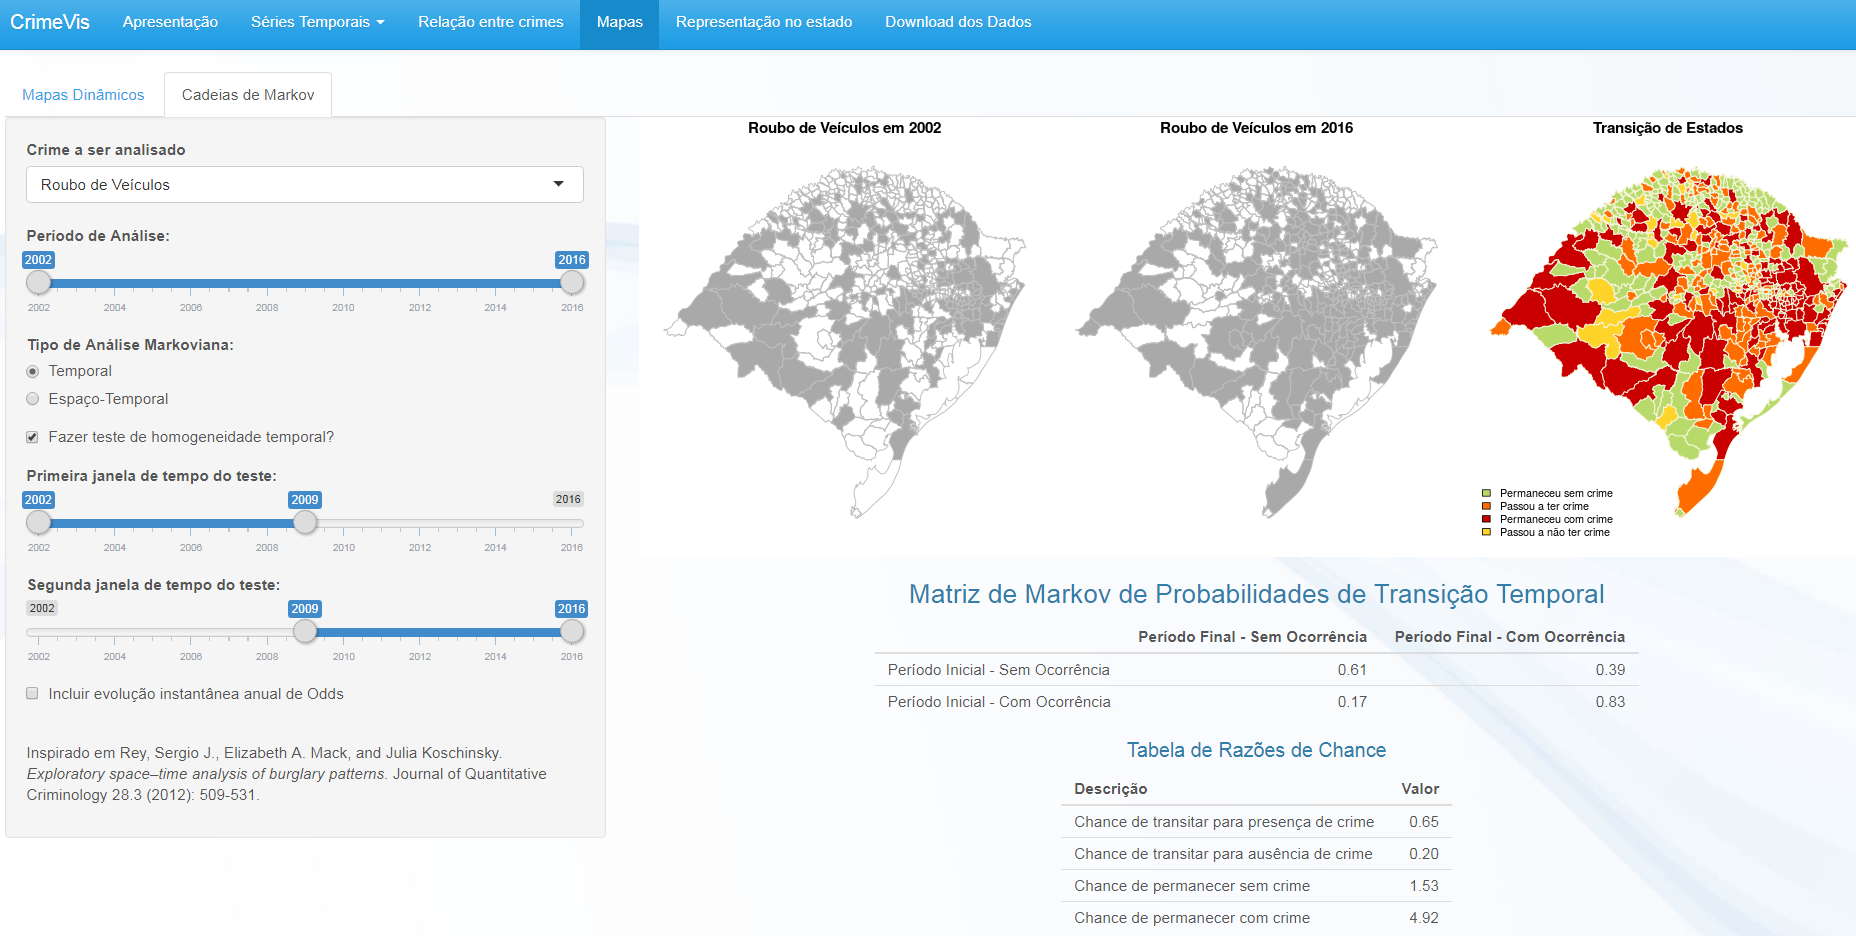
\includegraphics[width=1.00\linewidth]{screenshot_crimevis_temporal_com_testes.png}
  \caption{Mapas e cadeias temporais}
  \label{fig:acoplamento_crimevis_temp}
\end{subfigure} \\ % Quebra a linha para fazer os gráficos na vertical
\vspace{0.75cm} % Inclui um espaço em branco entre as figuras
\begin{subfigure}{.95\textwidth}
  \centering
  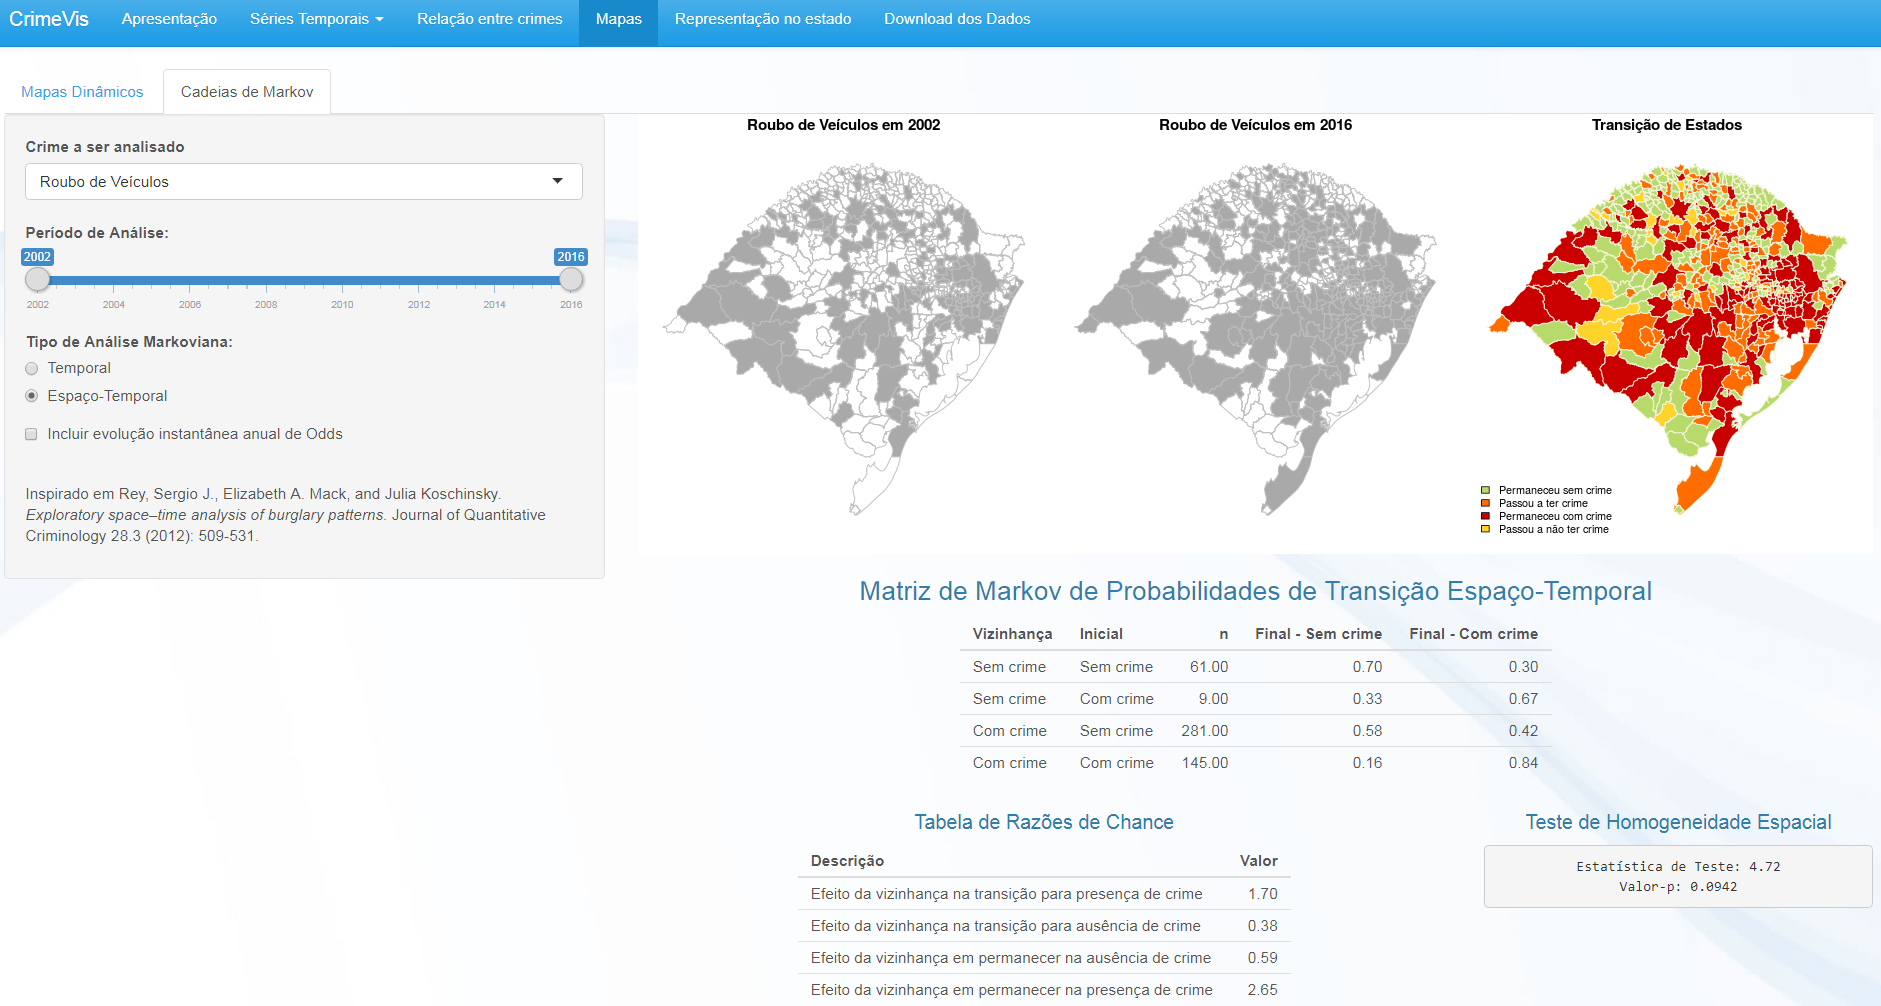
\includegraphics[width=1.00\linewidth]{screenshot_crimevis_espaco_temporal_com_testes.png}
  \caption{Mapas e cadeias espaço-temporais}
  \label{fig:acoplamento_crimevis_espaco_temp}
\end{subfigure}
\caption{Acoplamento dos modelos Markovianos no CrimeVis}
\label{fig:acoplamento_crimevis}
\end{center}
\end{figure}



É importante ressaltar que até onde se sabe não existe nenhum trabalho similar a este apresentado tanto em termos de análise markoviana espaço-temporal da criminalidade, quanto em sistematização desta abordagem em uma interface amigável que permite múltiplos tipos de cruzamentos. O CrimeVis faz uso conjunto do Shiny e da linguagem de programação \texttt{R} \cite{softwareR}, que representa uma poderosa ferramenta que possibilita diversos tipos de análise.

\section{Resultados\label{sec:resultados_acoplamento}}

\subsection{Estatísticas Descritivas Gerais\label{sec:esta_desc_markov}}

A Tabela \ref{tab:freq_mun_crime_markov} mostra a frequência de municípios que apresentaram pelo menos uma ocorrência de determinado crime para alguns anos selecionados da série histórica. Levando em consideração o fato de que no RS, entre 2002 e 2016, existem 496 municípios, a primeira característica notável é a assimetria da presença de determinados crimes nos municípios. Alguns crimes possuem ocorrências quase que na totalidade dos municípios, como é o caso de Furto (este está presente em todas as cidades em quase todos os anos), Roubo, Estelionato e Furto de Veículos. Por outro lado, alguns crimes são rarefeitos em termos de municípios em que ocorrem como Extorsão Mediante Sequestro, Latrocínio e Delitos Relacionados a Corrupção.

Outra característica marcante na tabela é a evolução temporal destas frequências. Em média, o número de municípios que apresentam os crimes é ascendente à medida que o tempo aumenta. Um destaque é o crime de Delitos Relacionados à Armas e Munições que teve um forte aumento entre 2002 e 2004. Este tipo de crime será discutido com mais detalhes posteriormente.

\begin{table}[H]
\begin{tiny}
\centering
\begin{tabular}{lrrrrrrrrr}
  \hline
Crime & 2002 & 2004 & 2006 & 2008 & 2010 & 2012 & 2014 & 2016 \\ 
  \hline
Delitos Relacionados à Armas e Munições & 21 & 434 & 416 & 426 & 426 & 446 & 427 & 436 \\ 
Delitos relacionados à Corrupção & 69 & 74 & 74 & 77 & 64 & 140 & 104 & 104 \\ 
Estelionato & 360 & 387 & 414 & 391 & 402 & 421 & 405 & 402 \\ 
Extorsão & 98 & 113 & 145 & 140 & 135 & 103 & 112 & 117 \\ 
Extorsão Mediante Sequestro & 7 & 10 & 15 & 8 & 11 & 10 & 24 & 9 \\ 
Furto & 486 & 496 & 496 & 496 & 496 & 496 & 496 & 496 \\ 
Furto de Veículos & 312 & 337 & 367 & 348 & 349 & 374 & 389 & 411 \\ 
Homicídio Doloso & 209 & 214 & 222 & 223 & 221 & 216 & 223 & 235 \\ 
Latrocínio & 47 & 44 & 61 & 38 & 43 & 47 & 60 & 68 \\ 
Posse de Entorpecentes & 218 & 232 & 222 & 250 & 265 & 276 & 309 & 310 \\ 
Roubo & 356 & 386 & 405 & 399 & 395 & 385 & 389 & 428 \\ 
Roubo de Veículos & 154 & 174 & 198 & 199 & 198 & 211 & 205 & 264 \\ 
Tráfico de Entorpecentes & 163 & 177 & 190 & 223 & 235 & 241 & 236 & 264 \\ 
   \hline
\end{tabular}
    \caption{Frequências de municípios que apresentaram crimes em anos selecionados}
    \label{tab:freq_mun_crime_markov}
\end{tiny}
\end{table}

Ao longo das próximas seções as análises serão realizadas para um subgrupo de crimes. Ademais, nos Apêndices \ref{appen:mapas_markov} e \ref{appen:prob_odds} diversas análises complementares estão presentes, que subsidiam as discussões que seguem.

\subsection{Roubo de Veículos\label{sec:roubo_de_veiculos_acoplamento}}

A Figura \ref{fig:mapas_roub_vei_markov_2002_2016} mostra a evolução temporal do roubo de veículos nos municípios do RS entre 2002 e 2016. Nesta figura, já apresentada na Seção \ref{sec:acomplamento_crimevis_acoplamento}, é possível perceber que as partes mais alaranjadas do mapa de transição de estados, que são municípios que não tiveram roubos, mas passaram a ter, estão localizados próximos à região metropolitana de Porto Alegre. Além disso, os municípios mais próximos a Porto Alegre apresentaram roubo nos dois períodos e, por isto, estão vermelhos.

% Este plot está todo customizado para o arquivo da tese, pois ele ajusta o tamanho da figura, width e height, recalcula o tamanho do título de cada plot e o tamanho da legenda (cex.main e cex)... grossura das linhas também lwd = 0.25
\begin{figure}[H]
\begin{center}
\includegraphics{TESE_DE_DOUTORADO_RENAN_FINAL-map_roub_vei_2002_2016}
\end{center}
\caption{Transição Espaço-Temporal markoviana do Roubo de Veículos entre 2002 e 2016}
\source{Fonte: Elaboração própria.}
\label{fig:mapas_roub_vei_markov_2002_2016}
\end{figure}

Esta característica aponta um processo de ''migração'' temporal para a região metropolitana de Porto Alegre. No entanto, em termos de quantificação desta mudança de dinâmica, as Tabelas \ref{tab:prob_tempo_roub_vei_2002_2016} e \ref{tab:odds_tempo_roub_vei_2002_2016} mostram, respectivamente as probabilidades de transição de estado e as razões de chance desta transição entre 2002 e 2016.

Na Tabela \ref{tab:prob_tempo_roub_vei_2002_2016} estão presentes as probabilidades de transição do estado inicial para o estado final. Se um município não apresentou crimes em 2002, é possível perceber que ele tem uma razoável probabilidade de 0,39 de passar a ter crimes em 2016. No entanto, se um município já apresentou crime no período inicial, a tendência é que ele se mantenha neste estado uma vez que a probabilidade de isto não se alterar é de 0,83. Em outras palavras, esta cadeia de Markov possui uma tendência maior dos municípios tenderem a ter crimes no futuro.

Esta interpretação fica mais clara quando analisamos as razões de chances através da Tabela \ref{tab:odds_tempo_roub_vei_2002_2016}. Nela podemos ver que a chance de permanecer em crime é de 4,92 e chance de transitar para a presença de crime é 0,65, que é maior do que a transição inversa (0,20).


\begin{table}[H]
\centering
\caption{Probabilidades de Transição Temporal do Roubo de Veículos entre 2002 e 2016}
        \begin{tabular}{ccc}
            \hline
            \multirow{2}{*}{Estado Inicial (2002)} & \multicolumn{2}{c}{Estado Final (2016)}  \\\cline{2-3} 
                                     & \multicolumn{1}{l}{Sem Crime} & \multicolumn{1}{l}{Com Crime} \\\hline
            {Sem Crime} & {0,61} & {0,39} \\                \hline
            {Com Crime} & {0,17} & {0,83} \\                \hline
            \tiny Fonte: Elaboração própria.
        \end{tabular}
    \label{tab:prob_tempo_roub_vei_2002_2016}
\end{table}

\begin{table}[H]
\centering
\caption{Razões de Chance Temporais do Roubo de Veículos entre 2002 e 2016}
        \begin{tabular}{lc}
            \hline
            {\textbf{Descrição}} & {\textbf{Razão de Chance}} \\\hline
            {Chance de transitar para presença de crime} & {0,65} \\
            {Chance de transitar para ausência de crime} & {0,20} \\
            {Chance de permanecer sem crime} & {1,53} \\
            {Chance de permanecer com crime} & {4,92} \\\hline
            \tiny Fonte: Elaboração própria.
        \end{tabular}
    \label{tab:odds_tempo_roub_vei_2002_2016}
\end{table}



As Tabelas espaço-temporais \ref{tab:prob_espaco_tempo_roub_vei_2002_2016} e \ref{tab:odds_espaco_tempo_roub_vei_2002_2016} permitem analisar a questão espaço-temporal do roubo de veículos entre 2002 e 2016 estratificando os municípios entre os que tiveram vizinhos com crimes em 2002 e os que não tiveram. O objetivo é avaliar se o fato de que se pelo menos um município vizinho teve roubo de veículos em 2002, afetaria o estado em 2016.

Primeiramente, nota-se a baixa frequência de municípios em que seus vizinhos não tiveram crimes em 2002 (apenas 70). Isto se configura um problema em termos inferenciais, tendo em vista o baixo poder que este estrato tem para estimar as probabilidades de transição, principalmente para os nove municípios que tiveram crime em 2002, mas que os vizinhos não tiveram. Desconsiderando esta limitação, vemos que a vizinhança afeta a probabilidade de transição para a presença de crimes. Transitar de \textit{SC} para \textit{CC} é 0,30 para o estrado \textit{Sem Crime} e 0,42 para o \textit{Com Crime}. Ou seja, existe um efeito positivo de que ter vizinhos com taxas de roubo implica em ter uma probabilidade maior de ter crimes no futuro, quando comparados com municípios que não tem vizinhos com este crime.

\begin{table}[H]
\centering
\caption{Probabilidades de Transição Espaço-Temporal do Roubo de Veículos entre 2002 e 2016}
        \begin{tabular}{ccccc}
            \hline
            \multirow{2}{*}{Vizinhança ($t_0$)} & \multirow{2}{*}{Estado Inicial (2002)} & \multirow{2}{*}{Freq.} & \multicolumn{2}{c}{Estado Final (2016)}  \\\cline{4-5} % As colunas 4 e 5 terão uma linha abaixo
                                        & & & \multicolumn{1}{l}{Sem Crime} & \multicolumn{1}{l}{Com Crime} \\\hline
            \multirow{2}{*}{Sem Crime} & {Sem Crime} & 61 &  {0,70} & {0,30} \\
                                       & {Com Crime} & 9 &   {0,33} & {0,67} \\\hline
            \multirow{2}{*}{Com Crime} & {Sem Crime} & 281 & {0,58} & {0,42} \\
                                       & {Com Crime} & 145 & {0,16} & {0,84} \\\hline
            \tiny Fonte: Elaboração própria.
        \end{tabular}
    \label{tab:prob_espaco_tempo_roub_vei_2002_2016}
\end{table}


Novamente, estas interpretações ficam mais claras quando olhamos as razões de chances que mensuram o efeito da vizinhança de 2002 na transição temporal $2002 \rightarrow 2016$. O valor mais interessante desta tabela é de que o efeito da vizinhança na transição de ausência para a presença de crime é 1,70 em termos de razão de chance. Outro valor importante é de que municípios que possuem vizinhos com crime tem 2,65 vezes a chance de permanecer em crime em relação aos municípios que não possuem. 


\begin{table}[H]
\centering
\caption{Razões de Chance Espaço-Temporais do Roubo de Veículos entre 2002 e 2016}
        \begin{tabular}{lc}
            \hline
            {\textbf{Descrição}} & {\textbf{Razão de Chance}} \\\hline
            {Efeito da vizinhança na transição para presença de crime} & {1,70} \\
            {Efeito da vizinhança na transição para ausência de crime} & {0,38} \\
            {Efeito da vizinhança em permanecer na ausência de crime} & {0,59} \\
            {Efeito da vizinhança em permanecer na presença de crime} & {2,65} \\\hline
            \tiny Fonte: Elaboração própria.
        \end{tabular}
    \label{tab:odds_espaco_tempo_roub_vei_2002_2016}
\end{table}


Esta dinâmica espaço-temporal de migração do Roubo de Veículos para a região metropolitana de Porto Alegre é interessante de inspecionar mais detalhadamente\footnote{Estes resultados estão apresentados nos apêndices.}. A fim de verificar a localização temporal destas variações de migração, dois subperíodos foram inspecionados: 2002-2009 e 2009-2016. Nota-se que a cadeia de Markov é mais estável para o subperíodo de 2002-2009, uma vez que a probabilidade de permanecer sem crime é de 0,73, de permanecer com crime é de 0,74 e a de transitar para a presença de crime é somente de 0,27. No entanto, sob a ótica do subperíodo 2009-2016 vemos que as transições para a presença de crime são mais preponderantes, uma vez que o mapa de transição é mais avermelhado e alaranjado. A probabilidade de transição para a presença de crimes salta para 0,34. No entanto, estes resultados de heterogeneidade temporal só são significativos com $\alpha = 10\%$ (Valor-p = 0,0626). Isto é, seguindo o teste temporal descrito na Seção \ref{sec:testes_acoplamento}, com 10\% de significância, rejeitamos a hipótese de que as probabilidades de transição entre 2002-2009 são equivalentes às probabilidades do período 2009-2016.

Uma das principais hipóteses que podem explicar esta transição acentuada de ausência de roubo de veículos para a presença é o fato de que a frota total de veículos de passageiros (assim como a frota total) quase dobrou no período 2002-2016, enquanto que a população do RS aumentou somente 8\%. Este aumento do número de veículos pode ter sido motivado pelas políticas de incentivo à demanda, como redução de IPI para veículos automotores que se deu a partir 2008. Sendo assim, é razoável supor que se existem mais carros em circulação, existe uma probabilidade maior de ocorrerem roubos de veículos. A Figura \ref{fig:evolu_frota_2002_2016} apresenta o número de veículo de passageiros para cada 100 habitantes no RS, que saltou de 24,55 em 2002 para 45,15 em 2016. 

Sob esta hipótese de que o aumento da frota possa ter afetado a ''migração'' do roubo de veículos a partir de 2008, outras duas janelas de tempo foram utilizadas para comparação temporal a fim de identificar valores mais significativos deslocando as janelas comparativas. De fato, quando comparamos 2002-2007 em relação a 2009-2016 a homogeneidade temporal é fortemente rejeitada a 1\% (Valor-p = 0,0066)\footnote{Quando analisamos outras janelas de subperíodos como, por exemplo, 2002-2008 em relação 2009-2016 ou 2002-2008 em relação 2008-2016 as altas significâncias se mantêm tendo valores-p iguais a 0,0098 e 0,0117, respectivamente.}. Sendo assim, corrobora-se esta hipótese da evolução da frota e esta análise está em consonância com os resultados das diferentes matrizes de transição dos subperíodos.

\begin{figure}[H]
\begin{center}
\includegraphics{TESE_DE_DOUTORADO_RENAN_FINAL-evo_frota}
\end{center}
\caption{Evolução da frota de veículos de passageiros por 100 habitantes no RS entre 2002 e 2016}
\source{Fonte: Fundação de Economia e Estatística e Detran-RS.}
\label{fig:evolu_frota_2002_2016}
\end{figure}


Em termos de relação espaço-temporal, apesar de haver indícios de que a vizinhança que teve crime no período inicial afeta positivamente a transição (ou permanência) nos crimes, ela não se mostrou significativa (para $\alpha = 5\%$) nem para o período 2002-2016 (Valor-p = 0,0942), nem para período 2009-2016 (Valor-p = 0,4416), enquanto que houve significância para o primeiro período 2002-2009 (Valor-p = 0,0157). Ademais, o efeito mais recente entre o período 2015-2016 é significativo (Valor-p = 0,0473) onde o efeito da vizinhança na transição para presença de crime é 3,75.


\subsection{Homicídio Doloso\label{sec:homicidio_acoplamento}}

O homicídio doloso tende a ser o tipo de crime mais utilizado na mensuração da criminalidade de determinada região, pois, assim como o roubo e furto de veículos, ele é um dos tipos de crime que menos sofre com os problemas de subnotificação \cite{cerqueira2014tese}. Por este motivo, ele é analisado no presente ensaio.

Analisando a dinâmica espaço-temporal entre 2002 e 2016, é posível notar a grande estabilidade regional que existe ao longo dos anos neste tipo de crime. Muitos municípios possuem a tendência de não mudar de estado, seja para permanecer sem crime ou para permanecer com crime. Além disso, esta análise possui um claro padrão espacial em que a região norte do RS é menos violenta e a região sul é mais violenta. A matriz de transição temporal de probabilidade apresenta altos valores na sua diagonal principal sendo 0,72 a probabilidade de se manter sem crime e 0,75 de se manter com crime. Em termos de razões de chances estimadas temos 2,63 e 2,94, respectivamente.

Observando os subperíodos do homicídio doloso, novamente, três janelas de tempo foram estimadas: 2002-2009 (primeira metade da série histórica), 2009-2016 (segunda metade) e efeito de transição mais recente (2015-2016). A principal característica é a estabilidade temporal entre diferentes subperíodos. O mesmo comportamento de alta chance de permanecer no estado inicial é observado em todos os subperíodos escolhidos. Ademais, o padrão espacial que divide o estado entre metade norte (menos criminosa) e metade sul (mais criminosa) também é notável ao longo do tempo. Em termos inferenciais, a hipótese de homogeneidade temporal não pode ser rejeitada quando comparamos diversos pares de anos, como, por exemplo, o subperíodo 2002-2009 com 2009-2016 (Valor-p = 0,127) e 2002-2009 com 2015-2016 (Valor-p = 0,2721).

No entanto, o resultado mais interessante na análise do homicídio doloso é o grande efeito pontual da vizinhança na criminalidade. O fato de ter vizinhos com crimes afeta em 9,30 a chance de permanecer em crime no futuro e a chance de transitar para a presença de crime é estimada em um fator de 1,74. Este resultado, mostra o efeito conjunto espaço-temporal da criminalidade homicida no RS, apontando uma evidência de que, se um município teve vizinhos violentos no passado, provavelmente este município apresentará crimes no futuro. Estes resultados só foram significativos a 10\% (Valor-p = 0,052).

Em termos de medida espaço-temporal, o período mais recente fornece boas pistas de como vizinhos com crimes podem afetar negativamente a taxa de homicídio. Com uma alta significância (Valor-p = 0,0113), observa-se que o efeito da vizinhança na transição para presença de crime é de 4,70 e o efeito da vizinhança em permanecer na presença de crime é de 6,67. Ou seja, em um período mais recente (2015-2016) existe esta forte indicação de como que a dinâmica espaço-temporal irá se dar em um período futuro como 2016-2017, por exemplo.

\subsection{Delitos relacionados à Armas e Munições\label{sec:armas_acoplamento}}

O crime de Delitos relacionados à Armas e Munições se referem aos crimes de \textit{Porte ilegal de arma de fogo de uso permitido, omissão de cautela de arma de fogo, disparo de arma de fogo, comércio ilegal de arma de fogo de uso permitido e posse ou porte ilegal de arma de fogo de uso restrito}. Adicionalmente, a sua dinâmica espaço-temporal possui uma característica interessante para ser analisada.

Quando se analisa conjuntamente os mapas de ocorrências municipais entre 2002 e 2016 e de transição de estados, vemos uma mudança abrupta de disposição criminal em todos os municípios gaúchos. A probabilidade de, condicionado a estar sem crimes no período inicial, passar a ter crimes no período final é de 0,88, resultando um mapa de transição quase totalmente laranja ($Sem \ Crime \rightarrow Com \ Crime$).

Um olhar mais cuidadoso em termos de taxas de ocorrências desta classe de crime foi conduzido observando a série histórica do estado e dos seus cinco maiores municípios e identificou-se uma nítida quebra de tendência entre os anos de 2003 e de 2004, também identificada e analisada em \co{menezes2017relaccoes}. Esta quebra se deu devido ao Estatuto do Desarmamento\footnote{\url{https://pt.wikipedia.org/wiki/Estatuto_do_Desarmamento} - Acesso em 18/11/2017} que entrou em vigor em 23 de dezembro de 2003 impondo novas regras concernentes a registro, posse e comercialização de armas de fogo e munição. A lei restringiu o porte de armas por civis, com exceção para os casos onde haja necessidade comprovada, o que nitidamente implicou em um aumento do número de ocorrências desta classe para o ano de 2004.

Em termos temporais, esta quebra entre 2003 e 2004 é evidente quando olhamos os três pares de anos 2002-2003, 2003-2004 e 2004-2005. No primeiro par de anos, a cadeia é estável onde a probabilidade de se manter sem crime, condicionado ao fato de também não ter crime no período inicial, é de 0,82. No segundo par de anos ocorre uma mudança abrupta na probabilidade de transitar para a presença de crimes, que passou para 0,84. Por fim, no par 2004-2005, a cadeia volta à estabilidade uma vez que a maioria dos municípios apresentam este tipo de ocorrência nos dois anos\footnote{Este crime impossibilita a estimação dos efeitos de vizinhança espaço-temporal, devido a ausência de múltiplos tipos de casos. Por este motivo, os resultados não são discutidos aqui.}. Em relação à inferência da homogeneidade temporal, ela é altamente rejeitada quando comparamos, por exemplo, o subintervalo 2002-2003 com 2003-2005 (Valor-p < 0,001 e $\chi^2 = 385,19$)\footnote{O subintervalo 2003-2004 não pode ser testado uma vez que não apresenta municípios que tiveram delito em 2003, mas não em 2004.}.

Uma das características interessantes de avaliar este crime em termos de efeitos da política do desarmamento de 2003 é estudar a dinâmica dos homicídios dolosos após 2003. Diversos estudos buscam avaliar os efeitos de armas de fogo, bem como o efeito do Estatuto do Desarmamento brasileiro, na criminalidade, como \co{hartung2011papel}, \co{dos2012avaliaccao}, \co{cerqueira2013evaluating}, \co{cerqueira2014tese}, \co{rostirolla2016mono} e \co{donohue2017right}\footnote{Alguns dos principais artigos que avaliaram a questão do Estatuto do Desarmamento no caso brasileiro estão reunidos no manifesto disponível em \url{https://igarape.org.br/manifesto-contra-a-revogacao-do-estatuto-do-desarmamento/} - Acesso em 18/11/2017.}\footnote{Uma boa revisão de literatura pode ser encontrada aqui \url{http://thomasvconti.com.br/2017/dossie-armas-violencia-e-crimes-o-que-nos-dizem-61-pesquisas-recentes} - Acesso em 18/11/2017.}. 

Neste sentido, sob a hipótese de que o estatuto afetou os homicídios\footnote{A literatura também relaciona outras variáveis como causadoras de homicídios.}, foi de interesse neste trabalho verificar o que houve com as cadeias de Markov com o homicídio doloso após o ano de 2003. Para isso, fixou-se o ano de 2003 e subperíodos foram construídos com o objetivo de comparar as diferentes chances de transição entre passar a ter (ou não) crime. Em termos comparativos, antes do Estatuto do Desarmamento, em 2002-2003, a chance de transitar para a presença de crime era maior que o contrário (0,37 em relação a 0,36). No entanto, após 2003, esta relação se inverte para 0,29 (chance de transitar para presença de crime) e 0,50 (chance de transitar para ausência de crime) em relação a 2004\footnote{Posteriormente, esta relação se mantém sendo 0,29 e 0,55 para 2003-2005; 0,26 e 0,39 para 2003-2006; 0,29 e 0,53 para 2003-2007; 0,35 e 0,50 para 2003-2008; 0,27 e 0,53 para 2003-2009; 0,33 e 0,49 para 2003-2010; 0,29 e 0,54 para 2003-2011; 0,31 e 0,52 para 2003-2012; 0,33 e 0,57 para 2003-2013; 0,31 e 0,45 para 2003-2014; 0,39 e 0,52 para 2003-2015 e 0,32 e 0,36 para 2003-2016.}.


\subsection{Tráfico de Entorpecentes\label{sec:trafico_acoplamento}}

O tráfico de entorpecentes apresenta uma dinâmica espaço-temporal de alta similaridade com a dos homicídios. Analisando o período 2002-2016, verificamos que existe uma diferenciação entre a região norte e a região sul do RS. Apesar de haver diversos municípios que passaram a ter tráfico (áreas laranjas no mapa de transição), a região norte é predominantemente verde, enquanto que a região sul possui o vermelho como cor mais frequente. A estreita relação entre tráficos e homicídios também é apontada em \co{beato2001conglomerados} e \co{menezes2017relaccoes}.

Este crime apresenta um razoável grau de estabilidade de transição uma vez que a probabilidade de se manter sem crime é de 0,65 e a probabilidade de se manter com crime é de 0,90. Esta estabilidade também é encontrada quando analisamos subperíodos da série histórica, pois entre 2002-2009 mostrou probabilidades de 0,75 e 0,87 e entre 2009-2016 de 0,74 e 0,87. Consequentemente, o teste de homogeneidade temporal resulta em alta estabilidade para estes dois subperíodos (Valor-p = 0,942).  Além disso, a análise espaço-temporal, a fim de estudar o efeito de ter municípios que possuem tráfico na transição temporal, não foi significativa em nenhum subperíodo. No entanto, valores pontuais altos foram estimados para o período completo, como o efeito da vizinhança na transição para presença de crime (1,52) e o efeito da vizinhança em permanecer na presença de crime (5,00).


\subsection{Outros Crimes\label{sec:outros_crimes_acoplamento}}

Alguns crimes específicos possuem características idiossincráticas em relação a base de dados. Primeiramente, analisamos que o Furto é o delito que, além de ser o que mais tem frequência em termos de ocorrência no RS, possui o maior grau de pulverização nos municípios. Quando comparamos os anos de 2002 e 2016 vimos os municípios, se manterem em estado de crime ou passarem a ter crimes, fazendo com que todo o mapa de transição seja vermelho, com apenas algumas regiões alaranjadas. Em outras palavras, todos os 496 municípios tiveram furto em 2016, o que inviabiliza os cálculos de probabilidades de transição temporal e espaço-temporal.

Em contrapartida, para este período, os crimes de latrocínio e de extorsão mediante sequestro possuem uma característica de prevalência rarefeita. Em ambos os casos, o mapa de transição é predominantemente verde. Em relação ao Latrocínio, a chance de um município permanecer sem crime é de 8,55 e existe um alto efeito espacial dos vizinhos. Existem evidências fortes e significativas (Valor-p = 0,0028) de que possuir vizinhos com latrocínio afeta tanto a transição para ter crimes (2,61) quanto a para permanecer com crimes (2,50). A extorsão mediante sequestro é mais rarefeita ainda e a chance de permanecer sem crimes é de 60,12.


\section{Considerações Finais\label{sec:consideracoes_finais_acoplamento}}

Este artigo realizou uma análise detalhada de como modelos de transição markovianos podem auxiliar a entender a dinâmica tanto espacial quanto temporal nos municípios do Rio Grande do Sul (RS). A variável sob análise foi uma variável dicotômica (\textit{dummy}) indicando se o município teve pelo menos uma ocorrência de determinado crime. Seguindo \co{rey2012exploratory}, fez-se uso de cadeias de Markov temporais que analisam a probabilidade de transição entre um estado de um período inicial para um final e fazendo a análise conjunta espaço-temporal estratificando a amostra em cidades que tiveram (ou não) municípios vizinhos com criminalidade. Diversos mapas, probabilidades, razões de chances e testes de hipóteses de homogeneidade temporais e espaciais foram conduzidos. Adicionalmente, este artigo mostrou como que estas medidas estão dispostas na ferramenta de visualização de dados dos crimes no RS, CrimeVis.

Após realizar algumas estatísticas descritivas, alguns crimes específicos foram analisados como roubo de veículos, homicídios dolosos, delitos relacionados à armas e munições e tráfico de entorpecentes. Cada um dos diferentes tipos de delitos apresentaram características específicas. Identificou-se um forte aumento das ocorrências de roubo de veículos para os municípios próximos à Região Metropolitana de Porto Alegre. Muitos municípios ''migraram'' de um estado de ausência de roubo de veículos para a presença. Uma das hipóteses levantadas para esta pulverização foram as políticas de incentivo ao consumo de veículos automotores aplicadas no Brasil no ano de 2008, principalmente devido ao fato de que quando comparamos os períodos anteriores e subsequentes deste ano, rejeitamos fortemente a hipótese de homogeneidade temporal. Em relação à análise espaço-temporal, o principal resultado, para os anos mais recentes de 2015 e 2016, aponta significativamente o efeito de ter vizinhos que apresentaram roubos de veículos com o intuito de prever o comportamento futuro. O efeito da vizinhança na transição para presença de crime e em permanecer na presença de crime são, respectivamente, 3,75 e 3,39, medidos através de razões de chance.

O segundo crime analisado foi o homicídio doloso, que apresentou uma grande estabilidade temporal e um padrão que divide o estado na metade norte (municípios com maior ausência) e metade sul (municípios com maior presença). No entanto, o principal resultado foi o grande efeito negativo que vizinhos que possuem crime desempenham na transição espaço-temporal. Foi identificado que possuir vizinhos com homicídio doloso, implica na chance de permanecer na presença de crime de 9,30 e de transitar para presença de crime de 1,74. Crimes relacionados à armas e munições também foi objeto de estudo, onde apresentaram uma grande quebra estrutural principalmente entre os anos de 2003 e 2004 provavelmente devido à vigência do Estatuto do Desarmamento vigorada a partir de 2003. Uma hipótese sobre o efeito subsequente desta lei também foi levantada nas transições dos homicídios dolosos após 2003. Por fim, o último crime que foi mais detalhado foi o tráfico de entorpecentes, que mostrou grande similaridade com os crimes de homicídios dolosos, tanto em termos de estabilidade temporal e de divisão regional no RS.

O acoplamento na ferramenta CrimeVis dos modelos temporais e espaço-temporais discutidos neste artigo mostrou-se muito importante, na medida em que é possível interagir com todas as possíveis abordagens para diferentes crimes e combinações de pares de anos em um único ambiente com uma interface amigável e intuitiva. Todas as análises investigadas aqui, assim como outras que o leitor possa querer realizar, podem ser acessadas gratuitamente através do site desta ferramenta em \href{http://visualiza.fee.tche.br/crime}{visualiza.fee.tche.br/crime}\footnote{Acesso em 19/11/2017.}.

Com relação a trabalhos futuros, diversas extensões de análises podem ser conduzidas. A principal limitação identificada é a de que, possivelmente, a medida de presença/ausência de crimes não seja a mais apropriada para analisar os municípios do RS a nível anual. Esta medida não leva em consideração o número bruto de ocorrências de determinada região, o que pode distorcer a compreensão espaço-temporal. Uma medida alternativa para ser investigada é a criação de uma variável \textit{dummy} que assuma o valor um caso a região esteja acima da média do estado daquele período e zero caso contrário. No entanto, esta medida também possui algumas desvantagens como, por exemplo, o fato do valor de comparação também ser dinâmico com o tempo. Além disso, cadeias de Markov podem ser estendidas para o caso em que a variável pode assumir mais de dois estados, o que poderia implicar em diferentes níveis de criminalidade, ao invés de apenas medir a presença/ausência de crime. Outra possível extensão é comparar a cadeia de transição das células com a cadeia de transição de seus respectivos vizinhos. Para isso, é necessária a criação de cadeias de Markov \textit{conjuntas} que avaliam a transição tanto das células propriamente ditas (cadeia \textit{própria}), quanto a transição de seus vizinhos (cadeia de \textit{vizinhança}) e assim testar se elas podem ser separáveis na medida em que a transição de uma célula seria independente da transição de seus vizinhos.

Apesar de diversos horizontes possíveis a serem explorados com cadeias de Markov na criminalidade gaúcha, acredita-se na importância do pioneirismo do presente trabalho, uma vez que, até onde se sabe, nenhum trabalho deste tipo foi feito para o RS. Além disso, todas estas abordagens sistematizadas em uma interface representam um passo importante para a segurança pública do estado e para trabalhos acadêmicos futuros.






\begin{subappendices}
\chapter*{Apêndice}
\addcontentsline{toc}{chapter}{Apêndice}
\section{Resultados temporais e espaço-temporais selecionados para a discussão entre mapas\label{appen:mapas_markov}}

Este apêndice apresenta mapas suplementares dos crimes e períodos selecionados para subsidiar as análises da Seção \ref{sec:esta_desc_markov} e, além disso, mostra a evolução das ocorrências dos Delitos Relacionados à Armas e Munições.

\begin{figure}[H]
\begin{center}
\includegraphics{TESE_DE_DOUTORADO_RENAN_FINAL-map_roub_vei_2002_2009}
\end{center}
\caption{Transição Espaço-Temporal markoviana do Roubo de Veículos entre 2002 e 2009}
\source{Fonte: Elaboração própria.}
\label{fig:mapas_roub_vei_markov_2002_2009}
\end{figure}


\begin{figure}[H]
\begin{center}
\includegraphics{TESE_DE_DOUTORADO_RENAN_FINAL-map_roub_vei_2009_2016}
\end{center}
\caption{Transição Espaço-Temporal markoviana do Roubo de Veículos entre 2009 e 2016}
\source{Fonte: Elaboração própria.}
\label{fig:mapas_roub_vei_markov_2009_2016}
\end{figure}

\begin{figure}[H]
\begin{center}
\includegraphics{TESE_DE_DOUTORADO_RENAN_FINAL-map_roub_vei_2015_2016}
\end{center}
\caption{Transição Espaço-Temporal markoviana do Roubo de Veículos entre 2015 e 2016}
\source{Fonte: Elaboração própria.}
\label{fig:mapas_roub_vei_markov_2015_2016}
\end{figure}

\begin{figure}[H]
\begin{center}
\includegraphics{TESE_DE_DOUTORADO_RENAN_FINAL-map_hom_dol_2002_2016}
\end{center}
\caption{Transição Espaço-Temporal markoviana do Homicídio Doloso entre 2002 e 2016}
\source{Fonte: Elaboração própria.}
\label{fig:mapas_hom_dol_markov_2002_2016}
\end{figure}


\begin{figure}[H]
\begin{center}
\includegraphics{TESE_DE_DOUTORADO_RENAN_FINAL-map_hom_dol_2002_2009}
\end{center}
\caption{Transição Espaço-Temporal markoviana do Homicídio Doloso entre 2002 e 2009}
\source{Fonte: Elaboração própria.}
\label{fig:mapas_hom_dol_markov_2002_2009}
\end{figure}

\begin{figure}[H]
\begin{center}
\includegraphics{TESE_DE_DOUTORADO_RENAN_FINAL-map_hom_dol_2009_2016}
\end{center}
\caption{Transição Espaço-Temporal markoviana do Homicídio Doloso entre 2009 e 2016}
\source{Fonte: Elaboração própria.}
\label{fig:mapas_hom_dol_markov_2009_2016}
\end{figure}

\begin{figure}[H]
\begin{center}
\includegraphics{TESE_DE_DOUTORADO_RENAN_FINAL-map_hom_dol_2015_2016}
\end{center}
\caption{Transição Espaço-Temporal markoviana do Homicídio Doloso entre 2015 e 2016}
\source{Fonte: Elaboração própria.}
\label{fig:mapas_hom_dol_markov_2015_2016}
\end{figure}


% Nos delitos relacionados a armas e munições aumenta-se o width por causa do longo título dos mapas
\begin{figure}[H]
\begin{center}
\includegraphics{TESE_DE_DOUTORADO_RENAN_FINAL-map_del_rel_armas_2002_2016}
\end{center}
\caption{Transição Espaço-Temporal markoviana de Delitos Relacionados à Armas e Munições entre 2002 e 2016}
\source{Fonte: Elaboração própria.}
\label{fig:mapas_del_rel_armas_markov_2002_2016}
\end{figure}

\begin{figure}[H]
\centering
\includegraphics[height=5cm,width=0.65\linewidth]{armas_cinco_maiores_municipios.png}
\caption{Evolução da Taxa dos Delitos Relacionados à Armas e Munições do RS e dos seus cinco maiores municípios}
\label{fig:evolucao_armas_cinco_maiores}
\end{figure}

\begin{figure}[H]
\begin{center}
\includegraphics{TESE_DE_DOUTORADO_RENAN_FINAL-map_del_rel_armas_2002_2003}
\end{center}
\caption{Transição Espaço-Temporal markoviana de Delitos Relacionados à Armas e Munições entre 2002 e 2003}
\source{Fonte: Elaboração própria.}
\label{fig:mapas_del_rel_armas_markov_2002_2003}
\end{figure}

\begin{figure}[H]
\begin{center}
\includegraphics{TESE_DE_DOUTORADO_RENAN_FINAL-map_del_rel_armas_2003_2004}
\end{center}
\caption{Transição Espaço-Temporal markoviana de Delitos Relacionados à Armas e Munições entre 2003 e 2004}
\source{Fonte: Elaboração própria.}
\label{fig:mapas_del_rel_armas_markov_2003_2004}
\end{figure}

\begin{figure}[H]
\begin{center}
\includegraphics{TESE_DE_DOUTORADO_RENAN_FINAL-map_del_rel_armas_2004_2005}
\end{center}
\caption{Transição Espaço-Temporal markoviana de Delitos Relacionados à Armas e Munições entre 2004 e 2005}
\source{Fonte: Elaboração própria.}
\label{fig:mapas_del_rel_armas_markov_2004_2005}
\end{figure}

\begin{figure}[H]
\begin{center}
\includegraphics{TESE_DE_DOUTORADO_RENAN_FINAL-map_trafico_2002_2016}
\end{center}
\caption{Transição Espaço-Temporal markoviana de Tráfico de Entorpecentes entre 2002 e 2016}
\source{Fonte: Elaboração própria.}
\label{fig:mapas_trafico_markov_2002_2016}
\end{figure}

\begin{figure}[H]
\begin{center}
\includegraphics{TESE_DE_DOUTORADO_RENAN_FINAL-map_trafico_2002_2009}
\end{center}
\caption{Transição Espaço-Temporal markoviana de Tráfico de Entorpecentes entre 2002 e 2009}
\source{Fonte: Elaboração própria.}
\label{fig:mapas_trafico_markov_2002_2009}
\end{figure}

\begin{figure}[H]
\begin{center}
\includegraphics{TESE_DE_DOUTORADO_RENAN_FINAL-map_trafico_2009_2016}
\end{center}
\caption{Transição Espaço-Temporal markoviana de Tráfico de Entorpecentes entre 2009 e 2016}
\source{Fonte: Elaboração própria.}
\label{fig:mapas_trafico_markov_2009_2016}
\end{figure}

\begin{figure}[H]
\begin{center}
\includegraphics{TESE_DE_DOUTORADO_RENAN_FINAL-map_furto_2002_2016}
\end{center}
\caption{Transição Espaço-Temporal markoviana do Furto entre 2002 e 2016}
\source{Fonte: Elaboração própria.}
\label{fig:mapas_furto_markov_2002_2016}
\end{figure}

\begin{figure}[H]
\begin{center}
\includegraphics{TESE_DE_DOUTORADO_RENAN_FINAL-map_latro_2002_2016}
\end{center}
\caption{Transição Espaço-Temporal markoviana do Latrocínio entre 2002 e 2016}
\source{Fonte: Elaboração própria.}
\label{fig:mapas_latrocinio_markov_2002_2016}
\end{figure}

\begin{figure}[H]
\begin{center}
\includegraphics{TESE_DE_DOUTORADO_RENAN_FINAL-map_extoMS_2002_2016}
\end{center}
\caption{Transição Espaço-Temporal markoviana da Extorsão Mediante Sequestro entre 2002 e 2016}
\source{Fonte: Elaboração própria.}
\label{fig:mapas_extoMS_markov_2002_2016}
\end{figure}










\section{Probabilidades de transição e razões de chance temporais e espaço-temporais para crimes e períodos selecionados\label{appen:prob_odds}}

\begin{table}[H]
\centering
\caption{Probabilidades de Transição Temporal do Roubo de Veículos entre 2002 e 2009}
        \begin{tabular}{ccc}
            \hline
            \multirow{2}{*}{Estado Inicial (2002)} & \multicolumn{2}{c}{Estado Final (2009)}  \\\cline{2-3} 
                                     & \multicolumn{1}{l}{Sem Crime} & \multicolumn{1}{l}{Com Crime} \\\hline
            {Sem Crime} & {0,73} & {0,27} \\                \hline
            {Com Crime} & {0,26} & {0,74} \\                \hline
            \tiny Fonte: Elaboração própria.
        \end{tabular}
    \label{tab:prob_tempo_roub_vei_2002_2009}
\end{table}

\begin{table}[H]
\centering
\caption{Razões de Chance Temporais do Roubo de Veículos entre 2002 e 2009}
        \begin{tabular}{lc}
            \hline
            {\textbf{Descrição}} & {\textbf{Razão de Chance}} \\\hline
            {Chance de transitar para presença de crime} & {0,37} \\
            {Chance de transitar para ausência de crime} & {0,35} \\
            {Chance de permanecer sem crime} & {2,72} \\
            {Chance de permanecer com crime} & {2,85} \\\hline
            \tiny Fonte: Elaboração própria.
        \end{tabular}
    \label{tab:odds_tempo_roub_vei_2002_2009}
\end{table}


\begin{table}[H]
\centering
\caption{Probabilidades de Transição Espaço-Temporal do Roubo de Veículos entre 2002 e 2009}
        \begin{tabular}{ccccc}
            \hline
            \multirow{2}{*}{Vizinhança ($t_0$)} & \multirow{2}{*}{Estado Inicial (2002)} & \multirow{2}{*}{Freq.} & \multicolumn{2}{c}{Estado Final (2009)}  \\\cline{4-5} % As colunas 4 e 5 terão uma linha abaixo
                                        & & & \multicolumn{1}{l}{Sem Crime} & \multicolumn{1}{l}{Com Crime} \\\hline
            \multirow{2}{*}{Sem Crime} & {Sem Crime} & 61 &  {0,84} & {0,16} \\
                                       & {Com Crime} & 9 &   {0,56} & {0,44} \\\hline
            \multirow{2}{*}{Com Crime} & {Sem Crime} & 281 & {0,71} & {0,29} \\
                                       & {Com Crime} & 145 & {0,24} & {0,76} \\\hline
            \tiny Fonte: Elaboração própria.
        \end{tabular}
    \label{tab:prob_espaco_tempo_roub_vei_2002_2009}
\end{table}


\begin{table}[H]
\centering
\caption{Razões de Chance Espaço-Temporais do Roubo de Veículos entre 2002 e 2009}
        \begin{tabular}{lc}
            \hline
            {\textbf{Descrição}} & {\textbf{Razão de Chance}} \\\hline
            {Efeito da vizinhança na transição para presença de crime} & {2,10} \\
            {Efeito da vizinhança na transição para ausência de crime} & {0,25} \\
            {Efeito da vizinhança em permanecer na ausência de crime} & {0,48} \\
            {Efeito da vizinhança em permanecer na presença de crime} & {3,93} \\\hline
            \tiny Fonte: Elaboração própria.
        \end{tabular}
    \label{tab:odds_espaco_tempo_roub_vei_2002_2009}
\end{table}














\begin{table}[H]
\centering
\caption{Probabilidades de Transição Temporal do Roubo de Veículos entre 2009 e 2016}
        \begin{tabular}{ccc}
            \hline
            \multirow{2}{*}{Estado Inicial (2009)} & \multicolumn{2}{c}{Estado Final (2016)}  \\\cline{2-3} 
                                     & \multicolumn{1}{l}{Sem Crime} & \multicolumn{1}{l}{Com Crime} \\\hline
            {Sem Crime} & {0,66} & {0,34} \\                \hline
            {Com Crime} & {0,21} & {0,79} \\                \hline
            \tiny Fonte: Elaboração própria.
        \end{tabular}
    \label{tab:prob_tempo_roub_vei_2009_2016}
\end{table}

\begin{table}[H]
\centering
\caption{Razões de Chance Temporais do Roubo de Veículos entre 2009 e 2016}
        \begin{tabular}{lc}
            \hline
            {\textbf{Descrição}} & {\textbf{Razão de Chance}} \\\hline
            {Chance de transitar para presença de crime} & {0,53} \\
            {Chance de transitar para ausência de crime} & {0,26} \\
            {Chance de permanecer sem crime} & {1,90} \\
            {Chance de permanecer com crime} & {3,79} \\\hline
            \tiny Fonte: Elaboração própria.
        \end{tabular}
    \label{tab:odds_tempo_roub_vei_2009_2016}
\end{table}


\begin{table}[H]
\centering
\caption{Probabilidades de Transição Espaço-Temporal do Roubo de Veículos entre 2009 e 2016}
        \begin{tabular}{ccccc}
            \hline
            \multirow{2}{*}{Vizinhança ($t_0$)} & \multirow{2}{*}{Estado Inicial (2009)} & \multirow{2}{*}{Freq.} & \multicolumn{2}{c}{Estado Final (2016)}  \\\cline{4-5} % As colunas 4 e 5 terão uma linha abaixo
                                        & & & \multicolumn{1}{l}{Sem Crime} & \multicolumn{1}{l}{Com Crime} \\\hline
            \multirow{2}{*}{Sem Crime} & {Sem Crime} & 42 &  {0,74} & {0,26} \\
                                       & {Com Crime} & 8 &   {0,25} & {0,75} \\\hline
            \multirow{2}{*}{Com Crime} & {Sem Crime} & 248 & {0,64} & {0,36} \\
                                       & {Com Crime} & 198 & {0,21} & {0,79} \\\hline
            \tiny Fonte: Elaboração própria.
        \end{tabular}
    \label{tab:prob_espaco_tempo_roub_vei_2009_2016}
\end{table}


\begin{table}[H]
\centering
\caption{Razões de Chance Espaço-Temporais do Roubo de Veículos entre 2009 e 2016}
        \begin{tabular}{lc}
            \hline
            {\textbf{Descrição}} & {\textbf{Razão de Chance}} \\\hline
            {Efeito da vizinhança na transição para presença de crime} & {1,58} \\
            {Efeito da vizinhança na transição para ausência de crime} & {0,78} \\
            {Efeito da vizinhança em permanecer na ausência de crime} & {0,63} \\
            {Efeito da vizinhança em permanecer na presença de crime} & {1,28} \\\hline
            \tiny Fonte: Elaboração própria.
        \end{tabular}
    \label{tab:odds_espaco_tempo_roub_vei_2009_2016}
\end{table}

















\begin{table}[H]
\centering
\caption{Probabilidades de Transição Temporal do Roubo de Veículos entre 2015 e 2016}
        \begin{tabular}{ccc}
            \hline
            \multirow{2}{*}{Estado Inicial (2015)} & \multicolumn{2}{c}{Estado Final (2016)}  \\\cline{2-3} 
                                     & \multicolumn{1}{l}{Sem Crime} & \multicolumn{1}{l}{Com Crime} \\\hline
            {Sem Crime} & {0,69} & {0,31} \\                \hline
            {Com Crime} & {0,23} & {0,77} \\                \hline
            \tiny Fonte: Elaboração própria.
        \end{tabular}
    \label{tab:prob_tempo_roub_vei_2015_2016}
\end{table}

\begin{table}[H]
\centering
\caption{Razões de Chance Temporais do Roubo de Veículos entre 2015 e 2016}
        \begin{tabular}{lc}
            \hline
            {\textbf{Descrição}} & {\textbf{Razão de Chance}} \\\hline
            {Chance de transitar para presença de crime} & {0,44} \\
            {Chance de transitar para ausência de crime} & {0,31} \\
            {Chance de permanecer sem crime} & {2,26} \\
            {Chance de permanecer com crime} & {3,26} \\\hline
            \tiny Fonte: Elaboração própria.
        \end{tabular}
    \label{tab:odds_tempo_roub_vei_2015_2016}
\end{table}


\begin{table}[H]
\centering
\caption{Probabilidades de Transição Espaço-Temporal do Roubo de Veículos entre 2015 e 2016}
        \begin{tabular}{ccccc}
            \hline
            \multirow{2}{*}{Vizinhança ($t_0$)} & \multirow{2}{*}{Estado Inicial (2015)} & \multirow{2}{*}{Freq.} & \multicolumn{2}{c}{Estado Final (2016)}  \\\cline{4-5} % As colunas 4 e 5 terão uma linha abaixo
                                        & & & \multicolumn{1}{l}{Sem Crime} & \multicolumn{1}{l}{Com Crime} \\\hline
            \multirow{2}{*}{Sem Crime} & {Sem Crime} & 18 &  {0,89} & {0,11} \\
                                       & {Com Crime} & 6 &   {0,50} & {0,50} \\\hline
            \multirow{2}{*}{Com Crime} & {Sem Crime} & 235 & {0,68} & {0,32} \\
                                       & {Com Crime} & 237 & {0,23} & {0,77} \\\hline
            \tiny Fonte: Elaboração própria.
        \end{tabular}
    \label{tab:prob_espaco_tempo_roub_vei_2015_2016}
\end{table}


\begin{table}[H]
\centering
\caption{Razões de Chance Espaço-Temporais do Roubo de Veículos entre 2015 e 2016}
        \begin{tabular}{lc}
            \hline
            {\textbf{Descrição}} & {\textbf{Razão de Chance}} \\\hline
            {Efeito da vizinhança na transição para presença de crime} & {3,75} \\
            {Efeito da vizinhança na transição para ausência de crime} & {0,30} \\
            {Efeito da vizinhança em permanecer na ausência de crime} & {0,27} \\
            {Efeito da vizinhança em permanecer na presença de crime} & {3,39} \\\hline
            \tiny Fonte: Elaboração própria.
        \end{tabular}
    \label{tab:odds_espaco_tempo_roub_vei_2015_2016}
\end{table}




















\begin{table}[H]
\centering
\caption{Probabilidades de Transição Temporal do Homicídio Doloso entre 2002 e 2016}
        \begin{tabular}{ccc}
            \hline
            \multirow{2}{*}{Estado Inicial (2002)} & \multicolumn{2}{c}{Estado Final (2016)}  \\\cline{2-3} 
                                     & \multicolumn{1}{l}{Sem Crime} & \multicolumn{1}{l}{Com Crime} \\\hline
            {Sem Crime} & {0,72} & {0,28} \\                \hline
            {Com Crime} & {0,25} & {0,75} \\                \hline
            \tiny Fonte: Elaboração própria.
        \end{tabular}
    \label{tab:prob_tempo_hom_dol_2002_2016}
\end{table}

\begin{table}[H]
\centering
\caption{Razões de Chance Temporais do Homicídio Doloso entre 2002 e 2016}
        \begin{tabular}{lc}
            \hline
            {\textbf{Descrição}} & {\textbf{Razão de Chance}} \\\hline
            {Chance de transitar para presença de crime} & {0,38} \\
            {Chance de transitar para ausência de crime} & {0,34} \\
            {Chance de permanecer sem crime} & {2,63} \\
            {Chance de permanecer com crime} & {2,94} \\\hline
            \tiny Fonte: Elaboração própria.
        \end{tabular}
    \label{tab:odds_tempo_hom_dol_2002_2016}
\end{table}


\begin{table}[H]
\centering
\caption{Probabilidades de Transição Espaço-Temporal do Homicídio entre 2002 e 2016}
        \begin{tabular}{ccccc}
            \hline
            \multirow{2}{*}{Vizinhança ($t_0$)} & \multirow{2}{*}{Estado Inicial (2002)} & \multirow{2}{*}{Freq.} & \multicolumn{2}{c}{Estado Final (2016)}  \\\cline{4-5} % As colunas 4 e 5 terão uma linha abaixo
                                        & & & \multicolumn{1}{l}{Sem Crime} & \multicolumn{1}{l}{Com Crime} \\\hline
            \multirow{2}{*}{Sem Crime} & {Sem Crime} & 32 &  {0,81} & {0,19} \\
                                       & {Com Crime} & 4 &   {0,75} & {0,25} \\\hline
            \multirow{2}{*}{Com Crime} & {Sem Crime} & 255 & {0,71} & {0,29} \\
                                       & {Com Crime} & 205 & {0,24} & {0,76} \\\hline
            \tiny Fonte: Elaboração própria.
        \end{tabular}
    \label{tab:prob_espaco_tempo_hom_dol_2002_2016}
\end{table}


\begin{table}[H]
\centering
\caption{Razões de Chance Espaço-Temporais do Homicídio Doloso entre 2002 e 2016}
        \begin{tabular}{lc}
            \hline
            {\textbf{Descrição}} & {\textbf{Razão de Chance}} \\\hline
            {Efeito da vizinhança na transição para presença de crime} & {1,74} \\
            {Efeito da vizinhança na transição para ausência de crime} & {0,11} \\
            {Efeito da vizinhança em permanecer na ausência de crime} & {0,58} \\
            {Efeito da vizinhança em permanecer na presença de crime} & {9,30} \\\hline
            \tiny Fonte: Elaboração própria.
        \end{tabular}
    \label{tab:odds_espaco_tempo_hom_dol_2002_2016}
\end{table}










\begin{table}[H]
\centering
\caption{Probabilidades de Transição Temporal do Homicídio Doloso entre 2002 e 2009}
        \begin{tabular}{ccc}
            \hline
            \multirow{2}{*}{Estado Inicial (2002)} & \multicolumn{2}{c}{Estado Final (2009)}  \\\cline{2-3} 
                                     & \multicolumn{1}{l}{Sem Crime} & \multicolumn{1}{l}{Com Crime} \\\hline
            {Sem Crime} & {0,79} & {0,21} \\                \hline
            {Com Crime} & {0,30} & {0,70} \\                \hline
            \tiny Fonte: Elaboração própria.
        \end{tabular}
    \label{tab:prob_tempo_hom_dol_2002_2009}
\end{table}

\begin{table}[H]
\centering
\caption{Razões de Chance Temporais do Homicídio Doloso entre 2002 e 2009}
        \begin{tabular}{lc}
            \hline
            {\textbf{Descrição}} & {\textbf{Razão de Chance}} \\\hline
            {Chance de transitar para presença de crime} & {0,27} \\
            {Chance de transitar para ausência de crime} & {0,42} \\
            {Chance de permanecer sem crime} & {3,70} \\
            {Chance de permanecer com crime} & {2,37} \\\hline
            \tiny Fonte: Elaboração própria.
        \end{tabular}
    \label{tab:odds_tempo_hom_dol_2002_2009}
\end{table}


\begin{table}[H]
\centering
\caption{Probabilidades de Transição Espaço-Temporal do Homicídio entre 2002 e 2009}
        \begin{tabular}{ccccc}
            \hline
            \multirow{2}{*}{Vizinhança ($t_0$)} & \multirow{2}{*}{Estado Inicial (2002)} & \multirow{2}{*}{Freq.} & \multicolumn{2}{c}{Estado Final (2009)}  \\\cline{4-5} % As colunas 4 e 5 terão uma linha abaixo
                                        & & & \multicolumn{1}{l}{Sem Crime} & \multicolumn{1}{l}{Com Crime} \\\hline
            \multirow{2}{*}{Sem Crime} & {Sem Crime} & 32 &  {0,72} & {0,28} \\
                                       & {Com Crime} & 4 &   {0,25} & {0,75} \\\hline
            \multirow{2}{*}{Com Crime} & {Sem Crime} & 255 & {0,80} & {0,20} \\
                                       & {Com Crime} & 205 & {0,30} & {0,70} \\\hline
            \tiny Fonte: Elaboração própria.
        \end{tabular}
    \label{tab:prob_espaco_tempo_hom_dol_2002_2009}
\end{table}


\begin{table}[H]
\centering
\caption{Razões de Chance Espaço-Temporais do Homicídio Doloso entre 2002 e 2009}
        \begin{tabular}{lc}
            \hline
            {\textbf{Descrição}} & {\textbf{Razão de Chance}} \\\hline
            {Efeito da vizinhança na transição para presença de crime} & {0,65} \\
            {Efeito da vizinhança na transição para ausência de crime} & {1,27} \\
            {Efeito da vizinhança em permanecer na ausência de crime} & {1,53} \\
            {Efeito da vizinhança em permanecer na presença de crime} & {0,79} \\\hline
            \tiny Fonte: Elaboração própria.
        \end{tabular}
    \label{tab:odds_espaco_tempo_hom_dol_2002_2009}
\end{table}















\begin{table}[H]
\centering
\caption{Probabilidades de Transição Temporal do Homicídio Doloso entre 2009 e 2016}
        \begin{tabular}{ccc}
            \hline
            \multirow{2}{*}{Estado Inicial (2009)} & \multicolumn{2}{c}{Estado Final (2016)}  \\\cline{2-3} 
                                     & \multicolumn{1}{l}{Sem Crime} & \multicolumn{1}{l}{Com Crime} \\\hline
            {Sem Crime} & {0,73} & {0,27} \\                \hline
            {Com Crime} & {0,25} & {0,75} \\                \hline
            \tiny Fonte: Elaboração própria.
        \end{tabular}
    \label{tab:prob_tempo_hom_dol_2009_2016}
\end{table}

\begin{table}[H]
\centering
\caption{Razões de Chance Temporais do Homicídio Doloso entre 2009 e 2016}
        \begin{tabular}{lc}
            \hline
            {\textbf{Descrição}} & {\textbf{Razão de Chance}} \\\hline
            {Chance de transitar para presença de crime} & {0,38} \\
            {Chance de transitar para ausência de crime} & {0,33} \\
            {Chance de permanecer sem crime} & {2,65} \\
            {Chance de permanecer com crime} & {3,00} \\\hline
            \tiny Fonte: Elaboração própria.
        \end{tabular}
    \label{tab:odds_tempo_hom_dol_2009_2016}
\end{table}


\begin{table}[H]
\centering
\caption{Probabilidades de Transição Espaço-Temporal do Homicídio entre 2009 e 2016}
        \begin{tabular}{ccccc}
            \hline
            \multirow{2}{*}{Vizinhança ($t_0$)} & \multirow{2}{*}{Estado Inicial (2009)} & \multirow{2}{*}{Freq.} & \multicolumn{2}{c}{Estado Final (2016)}  \\\cline{4-5} % As colunas 4 e 5 terão uma linha abaixo
                                        & & & \multicolumn{1}{l}{Sem Crime} & \multicolumn{1}{l}{Com Crime} \\\hline
            \multirow{2}{*}{Sem Crime} & {Sem Crime} & 12 &  {0,92} & {0,08} \\
                                       & {Com Crime} & 12 &  {0,42} & {0,58} \\\hline
            \multirow{2}{*}{Com Crime} & {Sem Crime} & 276 & {0,72} & {0,28} \\
                                       & {Com Crime} & 196 & {0,24} & {0,76} \\\hline
            \tiny Fonte: Elaboração própria.
        \end{tabular}
    \label{tab:prob_espaco_tempo_hom_dol_2009_2016}
\end{table}


\begin{table}[H]
\centering
\caption{Razões de Chance Espaço-Temporais do Homicídio Doloso entre 2009 e 2016}
        \begin{tabular}{lc}
            \hline
            {\textbf{Descrição}} & {\textbf{Razão de Chance}} \\\hline
            {Efeito da vizinhança na transição para presença de crime} & {4,33} \\
            {Efeito da vizinhança na transição para ausência de crime} & {0,44} \\
            {Efeito da vizinhança em permanecer na ausência de crime} & {0,23} \\
            {Efeito da vizinhança em permanecer na presença de crime} & {2,26} \\\hline
            \tiny Fonte: Elaboração própria.
        \end{tabular}
    \label{tab:odds_espaco_tempo_hom_dol_2009_2016}
\end{table}















\begin{table}[H]
\centering
\caption{Probabilidades de Transição Temporal do Homicídio Doloso entre 2015 e 2016}
        \begin{tabular}{ccc}
            \hline
            \multirow{2}{*}{Estado Inicial (2015)} & \multicolumn{2}{c}{Estado Final (2016)}  \\\cline{2-3} 
                                     & \multicolumn{1}{l}{Sem Crime} & \multicolumn{1}{l}{Com Crime} \\\hline
            {Sem Crime} & {0,73} & {0,27} \\                \hline
            {Com Crime} & {0,29} & {0,71} \\                \hline
            \tiny Fonte: Elaboração própria.
        \end{tabular}
    \label{tab:prob_tempo_hom_dol_2015_2016}
\end{table}

\begin{table}[H]
\centering
\caption{Razões de Chance Temporais do Homicídio Doloso entre 2015 e 2016}
        \begin{tabular}{lc}
            \hline
            {\textbf{Descrição}} & {\textbf{Razão de Chance}} \\\hline
            {Chance de transitar para presença de crime} & {0,37} \\
            {Chance de transitar para ausência de crime} & {0,40} \\
            {Chance de permanecer sem crime} & {2,70} \\
            {Chance de permanecer com crime} & {2,49} \\\hline
            \tiny Fonte: Elaboração própria.
        \end{tabular}
    \label{tab:odds_tempo_hom_dol_2015_2016}
\end{table}


\begin{table}[H]
\centering
\caption{Probabilidades de Transição Espaço-Temporal do Homicídio entre 2015 e 2016}
        \begin{tabular}{ccccc}
            \hline
            \multirow{2}{*}{Vizinhança ($t_0$)} & \multirow{2}{*}{Estado Inicial (2015)} & \multirow{2}{*}{Freq.} & \multicolumn{2}{c}{Estado Final (2016)}  \\\cline{4-5} % As colunas 4 e 5 terão uma linha abaixo
                                        & & & \multicolumn{1}{l}{Sem Crime} & \multicolumn{1}{l}{Com Crime} \\\hline
            \multirow{2}{*}{Sem Crime} & {Sem Crime} & 13 &  {0,92} & {0,08} \\
                                       & {Com Crime} & 7 &   {0,71} & {0,29} \\\hline
            \multirow{2}{*}{Com Crime} & {Sem Crime} & 256 & {0,72} & {0,28} \\
                                       & {Com Crime} & 220 & {0,27} & {0,73} \\\hline
            \tiny Fonte: Elaboração própria.
        \end{tabular}
    \label{tab:prob_espaco_tempo_hom_dol_2015_2016}
\end{table}


\begin{table}[H]
\centering
\caption{Razões de Chance Espaço-Temporais do Homicídio Doloso entre 2015 e 2016}
        \begin{tabular}{lc}
            \hline
            {\textbf{Descrição}} & {\textbf{Razão de Chance}} \\\hline
            {Efeito da vizinhança na transição para presença de crime} & {4,70} \\
            {Efeito da vizinhança na transição para ausência de crime} & {0,15} \\
            {Efeito da vizinhança em permanecer na ausência de crime} & {0,21} \\
            {Efeito da vizinhança em permanecer na presença de crime} & {6,67} \\\hline
            \tiny Fonte: Elaboração própria.
        \end{tabular}
    \label{tab:odds_espaco_tempo_hom_dol_2015_2016}
\end{table}



















\begin{table}[H]
\centering
\caption{Probabilidades de Transição Temporal de Delitos Relacionados à Armas e Munições entre 2002 e 2016}
        \begin{tabular}{ccc}
            \hline
            \multirow{2}{*}{Estado Inicial (2002)} & \multicolumn{2}{c}{Estado Final (2016)}  \\\cline{2-3} 
                                     & \multicolumn{1}{l}{Sem Crime} & \multicolumn{1}{l}{Com Crime} \\\hline
            {Sem Crime} & {0,12} & {0,88} \\                \hline
            {Com Crime} & {0,05} & {0,95} \\                \hline
            \tiny Fonte: Elaboração própria.
        \end{tabular}
    \label{tab:prob_tempo_rel_arma_2002_2016}
\end{table}

\begin{table}[H]
\centering
\caption{Razões de Chance Temporais de Delitos Relacionados à Armas e Munições entre 2002 e 2016}
        \begin{tabular}{lc}
            \hline
            {\textbf{Descrição}} & {\textbf{Razão de Chance}} \\\hline
            {Chance de transitar para presença de crime} & {7,05} \\
            {Chance de transitar para ausência de crime} & {0,05} \\
            {Chance de permanecer sem crime} & {0,14} \\
            {Chance de permanecer com crime} & {20,00} \\\hline
            \tiny Fonte: Elaboração própria.
        \end{tabular}
    \label{tab:odds_tempo_rel_arma_2002_2016}
\end{table}


\begin{table}[H]
\centering
\caption{Probabilidades de Transição Espaço-Temporal de Delitos Relacionados à Armas e Munições entre 2002 e 2016}
        \begin{tabular}{ccccc}
            \hline
            \multirow{2}{*}{Vizinhança ($t_0$)} & \multirow{2}{*}{Estado Inicial (2002)} & \multirow{2}{*}{Freq.} & \multicolumn{2}{c}{Estado Final (2016)}  \\\cline{4-5} % As colunas 4 e 5 terão uma linha abaixo
                                        & & & \multicolumn{1}{l}{Sem Crime} & \multicolumn{1}{l}{Com Crime} \\\hline
            \multirow{2}{*}{Sem Crime} & {Sem Crime} & 373 &  {0,14} & {0,86} \\
                                       & {Com Crime} & 7   &  {0,14} & {0,86} \\\hline
            \multirow{2}{*}{Com Crime} & {Sem Crime} & 102 &  {0,07} & {0,93} \\
                                       & {Com Crime} & 14  &  {0,00} & {1,00} \\\hline
            \tiny Fonte: Elaboração própria.
        \end{tabular}
    \label{tab:prob_espaco_tempo_rel_arma_2002_2016}
\end{table}


\begin{table}[H]
\centering
\caption{Razões de Chance Espaço-Temporais de Delitos Relacionados à Armas e Munições entre 2002 e 2016}
        \begin{tabular}{lc}
            \hline
            {\textbf{Descrição}} & {\textbf{Razão de Chance}} \\\hline
            {Efeito da vizinhança na transição para presença de crime} & {2,20} \\
            {Efeito da vizinhança na transição para ausência de crime} & {0,00} \\
            {Efeito da vizinhança em permanecer na ausência de crime} & {0,45} \\
            {Efeito da vizinhança em permanecer na presença de crime} & {-} \\\hline
            \tiny Fonte: Elaboração própria.
        \end{tabular}
    \label{tab:odds_espaco_tempo_rel_arma_2002_2016}
\end{table}










\begin{table}[H]
\centering
\caption{Probabilidades de Transição Temporal de Delitos Relacionados à Armas e Munições entre 2002 e 2003}
        \begin{tabular}{ccc}
            \hline
            \multirow{2}{*}{Estado Inicial (2002)} & \multicolumn{2}{c}{Estado Final (2003)}  \\\cline{2-3} 
                                     & \multicolumn{1}{l}{Sem Crime} & \multicolumn{1}{l}{Com Crime} \\\hline
            {Sem Crime} & {0,82} & {0,18} \\                \hline
            {Com Crime} & {0,33} & {0,67} \\                \hline
            \tiny Fonte: Elaboração própria.
        \end{tabular}
    \label{tab:prob_tempo_rel_arma_2002_2003}
\end{table}

\begin{table}[H]
\centering
\caption{Razões de Chance Temporais de Delitos Relacionados à Armas e Munições entre 2002 e 2003}
        \begin{tabular}{lc}
            \hline
            {\textbf{Descrição}} & {\textbf{Razão de Chance}} \\\hline
            {Chance de transitar para presença de crime} & {0,22} \\
            {Chance de transitar para ausência de crime} & {0,50} \\
            {Chance de permanecer sem crime} & {4,59} \\
            {Chance de permanecer com crime} & {2,00} \\\hline
            \tiny Fonte: Elaboração própria.
        \end{tabular}
    \label{tab:odds_tempo_rel_arma_2002_2003}
\end{table}


\begin{table}[H]
\centering
\caption{Probabilidades de Transição Espaço-Temporal de Delitos Relacionados à Armas e Munições entre 2002 e 2003}
        \begin{tabular}{ccccc}
            \hline
            \multirow{2}{*}{Vizinhança ($t_0$)} & \multirow{2}{*}{Estado Inicial (2002)} & \multirow{2}{*}{Freq.} & \multicolumn{2}{c}{Estado Final (2003)}  \\\cline{4-5} % As colunas 4 e 5 terão uma linha abaixo
                                        & & & \multicolumn{1}{l}{Sem Crime} & \multicolumn{1}{l}{Com Crime} \\\hline
            \multirow{2}{*}{Sem Crime} & {Sem Crime} & 373 &  {0,86} & {0,14} \\
                                       & {Com Crime} & 7 &    {0,43} & {0,57} \\\hline
            \multirow{2}{*}{Com Crime} & {Sem Crime} & 102 &  {0,67} & {0,33} \\
                                       & {Com Crime} & 14 &   {0,29} & {0,71} \\\hline
            \tiny Fonte: Elaboração própria.
        \end{tabular}
    \label{tab:prob_espaco_tempo_rel_arma_2002_2003}
\end{table}


\begin{table}[H]
\centering
\caption{Razões de Chance Espaço-Temporais de Delitos Relacionados à Armas e Munições entre 2002 e 2003}
        \begin{tabular}{lc}
            \hline
            {\textbf{Descrição}} & {\textbf{Razão de Chance}} \\\hline
            {Efeito da vizinhança na transição para presença de crime} & {3,16} \\
            {Efeito da vizinhança na transição para ausência de crime} & {0,53} \\
            {Efeito da vizinhança em permanecer na ausência de crime} & {0,32} \\
            {Efeito da vizinhança em permanecer na presença de crime} & {1,88} \\\hline
            \tiny Fonte: Elaboração própria.
        \end{tabular}
    \label{tab:odds_espaco_tempo_rel_arma_2002_2003}
\end{table}


























\begin{table}[H]
\centering
\caption{Probabilidades de Transição Temporal de Delitos Relacionados à Armas e Munições entre 2003 e 2004}
        \begin{tabular}{ccc}
            \hline
            \multirow{2}{*}{Estado Inicial (2003)} & \multicolumn{2}{c}{Estado Final (2004)}  \\\cline{2-3} 
                                     & \multicolumn{1}{l}{Sem Crime} & \multicolumn{1}{l}{Com Crime} \\\hline
            {Sem Crime} & {0,16} & {0,84} \\                \hline
            {Com Crime} & {0,00} & {1,00} \\                \hline
            \tiny Fonte: Elaboração própria.
        \end{tabular}
    \label{tab:prob_tempo_rel_arma_2003_2004}
\end{table}

\begin{table}[H]
\centering
\caption{Razões de Chance Temporais de Delitos Relacionados à Armas e Munições entre 2003 e 2004}
        \begin{tabular}{lc}
            \hline
            {\textbf{Descrição}} & {\textbf{Razão de Chance}} \\\hline
            {Chance de transitar para presença de crime} & {5,40} \\
            {Chance de transitar para ausência de crime} & {0,00} \\
            {Chance de permanecer sem crime} & {0,19} \\
            {Chance de permanecer com crime} & {-} \\\hline
            \tiny Fonte: Elaboração própria.
        \end{tabular}
    \label{tab:odds_tempo_rel_arma_2003_2004}
\end{table}


\begin{table}[H]
\centering
\caption{Probabilidades de Transição Espaço-Temporal de Delitos Relacionados à Armas e Munições entre 2003 e 2004}
        \begin{tabular}{ccccc}
            \hline
            \multirow{2}{*}{Vizinhança ($t_0$)} & \multirow{2}{*}{Estado Inicial (2003)} & \multirow{2}{*}{Freq.} & \multicolumn{2}{c}{Estado Final (2004)}  \\\cline{4-5} % As colunas 4 e 5 terão uma linha abaixo
                                        & & & \multicolumn{1}{l}{Sem Crime} & \multicolumn{1}{l}{Com Crime} \\\hline
            \multirow{2}{*}{Sem Crime} & {Sem Crime} & 135 &  {0,13} & {0,87} \\
                                       & {Com Crime} & 16 &   {0,00} & {1,00} \\\hline
            \multirow{2}{*}{Com Crime} & {Sem Crime} & 262 &  {0,17} & {0,83} \\
                                       & {Com Crime} & 83 &   {0,00} & {1,00} \\\hline
            \tiny Fonte: Elaboração própria.
        \end{tabular}
    \label{tab:prob_espaco_tempo_rel_arma_2003_2004}
\end{table}


\begin{table}[H]
\centering
\caption{Razões de Chance Espaço-Temporais de Delitos Relacionados à Armas e Munições entre 2003 e 2004}
        \begin{tabular}{lc}
            \hline
            {\textbf{Descrição}} & {\textbf{Razão de Chance}} \\\hline
            {Efeito da vizinhança na transição para presença de crime} & {0,76} \\
            {Efeito da vizinhança na transição para ausência de crime} & {-} \\
            {Efeito da vizinhança em permanecer na ausência de crime} & {1,31} \\
            {Efeito da vizinhança em permanecer na presença de crime} & {-} \\\hline
            \tiny Fonte: Elaboração própria.
        \end{tabular}
    \label{tab:odds_espaco_tempo_rel_arma_2003_2004}
\end{table}















\begin{table}[H]
\centering
\caption{Probabilidades de Transição Temporal de Delitos Relacionados à Armas e Munições entre 2004 e 2005}
        \begin{tabular}{ccc}
            \hline
            \multirow{2}{*}{Estado Inicial (2004)} & \multicolumn{2}{c}{Estado Final (2005)}  \\\cline{2-3} 
                                     & \multicolumn{1}{l}{Sem Crime} & \multicolumn{1}{l}{Com Crime} \\\hline
            {Sem Crime} & {0,48} & {0,52} \\                \hline
            {Com Crime} & {0,11} & {0,89} \\                \hline
            \tiny Fonte: Elaboração própria.
        \end{tabular}
    \label{tab:prob_tempo_rel_arma_2004_2005}
\end{table}

\begin{table}[H]
\centering
\caption{Razões de Chance Temporais de Delitos Relacionados à Armas e Munições entre 2004 e 2005}
        \begin{tabular}{lc}
            \hline
            {\textbf{Descrição}} & {\textbf{Razão de Chance}} \\\hline
            {Chance de transitar para presença de crime} & {1,07} \\
            {Chance de transitar para ausência de crime} & {0,13} \\
            {Chance de permanecer sem crime} & {0,94} \\
            {Chance de permanecer com crime} & {7,86} \\\hline
            \tiny Fonte: Elaboração própria.
        \end{tabular}
    \label{tab:odds_tempo_rel_arma_2004_2005}
\end{table}
















\begin{table}[H]
\centering
\caption{Probabilidades de Transição Temporal de Tráfico de Entorpecentes entre 2002 e 2016}
        \begin{tabular}{ccc}
            \hline
            \multirow{2}{*}{Estado Inicial (2002)} & \multicolumn{2}{c}{Estado Final (2016)}  \\\cline{2-3} 
                                     & \multicolumn{1}{l}{Sem Crime} & \multicolumn{1}{l}{Com Crime} \\\hline
            {Sem Crime} & {0,65} & {0,35} \\                \hline
            {Com Crime} & {0,10} & {0,90} \\                \hline
            \tiny Fonte: Elaboração própria.
        \end{tabular}
    \label{tab:prob_tempo_trafico_2002_2016}
\end{table}

\begin{table}[H]
\centering
\caption{Razões de Chance Temporais de Tráfico de Entorpecentes entre 2002 e 2016}
        \begin{tabular}{lc}
            \hline
            {\textbf{Descrição}} & {\textbf{Razão de Chance}} \\\hline
            {Chance de transitar para presença de crime} & {0,55} \\
            {Chance de transitar para ausência de crime} & {0,12} \\
            {Chance de permanecer sem crime} & {1,82} \\
            {Chance de permanecer com crime} & {8,59} \\\hline
            \tiny Fonte: Elaboração própria.
        \end{tabular}
    \label{tab:odds_tempo_trafico_2002_2016}
\end{table}


\begin{table}[H]
\centering
\caption{Probabilidades de Transição Espaço-Temporal de Tráfico de Entorpecentes entre 2002 e 2016}
        \begin{tabular}{ccccc}
            \hline
            \multirow{2}{*}{Vizinhança ($t_0$)} & \multirow{2}{*}{Estado Inicial (2002)} & \multirow{2}{*}{Freq.} & \multicolumn{2}{c}{Estado Final (2016)}  \\\cline{4-5} % As colunas 4 e 5 terão uma linha abaixo
                                        & & & \multicolumn{1}{l}{Sem Crime} & \multicolumn{1}{l}{Com Crime} \\\hline
            \multirow{2}{*}{Sem Crime} & {Sem Crime} & 40 &  {0,72} & {0,28} \\
                                       & {Com Crime} & 9 &   {0,33} & {0,67} \\\hline
            \multirow{2}{*}{Com Crime} & {Sem Crime} & 293 & {0,63} & {0,37} \\
                                       & {Com Crime} & 154 & {0,09} & {0,91} \\\hline
            \tiny Fonte: Elaboração própria.
        \end{tabular}
    \label{tab:prob_espaco_tempo_trafico_2002_2016}
\end{table}


\begin{table}[H]
\centering
\caption{Razões de Chance Espaço-Temporais de Tráfico de Entorpecentes entre 2002 e 2016}
        \begin{tabular}{lc}
            \hline
            {\textbf{Descrição}} & {\textbf{Razão de Chance}} \\\hline
            {Efeito da vizinhança na transição para presença de crime} & {1,52} \\
            {Efeito da vizinhança na transição para ausência de crime} & {0,20} \\
            {Efeito da vizinhança em permanecer na ausência de crime} & {0,66} \\
            {Efeito da vizinhança em permanecer na presença de crime} & {5,00} \\\hline
            \tiny Fonte: Elaboração própria.
        \end{tabular}
    \label{tab:odds_espaco_tempo_trafico_2002_2016}
\end{table}














\begin{table}[H]
\centering
\caption{Probabilidades de Transição Temporal de Tráfico de Entorpecentes entre 2002 e 2009}
        \begin{tabular}{ccc}
            \hline
            \multirow{2}{*}{Estado Inicial (2002)} & \multicolumn{2}{c}{Estado Final (2009)}  \\\cline{2-3} 
                                     & \multicolumn{1}{l}{Sem Crime} & \multicolumn{1}{l}{Com Crime} \\\hline
            {Sem Crime} & {0,75} & {0,25} \\                \hline
            {Com Crime} & {0,13} & {0,87} \\                \hline
            \tiny Fonte: Elaboração própria.
        \end{tabular}
    \label{tab:prob_tempo_trafico_2002_2009}
\end{table}

\begin{table}[H]
\centering
\caption{Razões de Chance Temporais de Tráfico de Entorpecentes entre 2002 e 2009}
        \begin{tabular}{lc}
            \hline
            {\textbf{Descrição}} & {\textbf{Razão de Chance}} \\\hline
            {Chance de transitar para presença de crime} & {0,33} \\
            {Chance de transitar para ausência de crime} & {0,15} \\
            {Chance de permanecer sem crime} & {3,06} \\
            {Chance de permanecer com crime} & {6,76} \\\hline
            \tiny Fonte: Elaboração própria.
        \end{tabular}
    \label{tab:odds_tempo_trafico_2002_2009}
\end{table}


\begin{table}[H]
\centering
\caption{Probabilidades de Transição Espaço-Temporal de Tráfico de Entorpecentes entre 2002 e 2009}
        \begin{tabular}{ccccc}
            \hline
            \multirow{2}{*}{Vizinhança ($t_0$)} & \multirow{2}{*}{Estado Inicial (2002)} & \multirow{2}{*}{Freq.} & \multicolumn{2}{c}{Estado Final (2009)}  \\\cline{4-5} % As colunas 4 e 5 terão uma linha abaixo
                                        & & & \multicolumn{1}{l}{Sem Crime} & \multicolumn{1}{l}{Com Crime} \\\hline
            \multirow{2}{*}{Sem Crime} & {Sem Crime} & 40 &  {0,82} & {0,17} \\
                                       & {Com Crime} & 9 &   {0,33} & {0,67} \\\hline
            \multirow{2}{*}{Com Crime} & {Sem Crime} & 293 & {0,74} & {0,26} \\
                                       & {Com Crime} & 154 & {0,12} & {0,88} \\\hline
            \tiny Fonte: Elaboração própria.
        \end{tabular}
    \label{tab:prob_espaco_tempo_trafico_2002_2009}
\end{table}


\begin{table}[H]
\centering
\caption{Razões de Chance Espaço-Temporais de Tráfico de Entorpecentes entre 2002 e 2009}
        \begin{tabular}{lc}
            \hline
            {\textbf{Descrição}} & {\textbf{Razão de Chance}} \\\hline
            {Efeito da vizinhança na transição para presença de crime} & {1,62} \\
            {Efeito da vizinhança na transição para ausência de crime} & {0,26} \\
            {Efeito da vizinhança em permanecer na ausência de crime} & {0,62} \\
            {Efeito da vizinhança em permanecer na presença de crime} & {3,78} \\\hline
            \tiny Fonte: Elaboração própria.
        \end{tabular}
    \label{tab:odds_espaco_tempo_trafico_2002_2009}
\end{table}













\begin{table}[H]
\centering
\caption{Probabilidades de Transição Temporal de Tráfico de Entorpecentes entre 2009 e 2016}
        \begin{tabular}{ccc}
            \hline
            \multirow{2}{*}{Estado Inicial (2009)} & \multicolumn{2}{c}{Estado Final (2016)}  \\\cline{2-3} 
                                     & \multicolumn{1}{l}{Sem Crime} & \multicolumn{1}{l}{Com Crime} \\\hline
            {Sem Crime} & {0,74} & {0,26} \\                \hline
            {Com Crime} & {0,13} & {0,87} \\                \hline
            \tiny Fonte: Elaboração própria.
        \end{tabular}
    \label{tab:prob_tempo_trafico_2009_2016}
\end{table}

\begin{table}[H]
\centering
\caption{Razões de Chance Temporais de Tráfico de Entorpecentes entre 2009 e 2016}
        \begin{tabular}{lc}
            \hline
            {\textbf{Descrição}} & {\textbf{Razão de Chance}} \\\hline
            {Chance de transitar para presença de crime} & {0,35} \\
            {Chance de transitar para ausência de crime} & {0,15} \\
            {Chance de permanecer sem crime} & {2,89} \\
            {Chance de permanecer com crime} & {6,47} \\\hline
            \tiny Fonte: Elaboração própria.
        \end{tabular}
    \label{tab:odds_tempo_trafico_2009_2016}
\end{table}


\begin{table}[H]
\centering
\caption{Probabilidades de Transição Espaço-Temporal de Tráfico de Entorpecentes entre 2009 e 2016}
        \begin{tabular}{ccccc}
            \hline
            \multirow{2}{*}{Vizinhança ($t_0$)} & \multirow{2}{*}{Estado Inicial (2009)} & \multirow{2}{*}{Freq.} & \multicolumn{2}{c}{Estado Final (2016)}  \\\cline{4-5} % As colunas 4 e 5 terão uma linha abaixo
                                        & & & \multicolumn{1}{l}{Sem Crime} & \multicolumn{1}{l}{Com Crime} \\\hline
            \multirow{2}{*}{Sem Crime} & {Sem Crime} & 18 &  {0,78} & {0,22} \\
                                       & {Com Crime} & 6 &   {0,50} & {0,50} \\\hline
            \multirow{2}{*}{Com Crime} & {Sem Crime} & 254 & {0,74} & {0,26} \\
                                       & {Com Crime} & 218 & {0,12} & {0,88} \\\hline
            \tiny Fonte: Elaboração própria.
        \end{tabular}
    \label{tab:prob_espaco_tempo_trafico_2009_2016}
\end{table}


\begin{table}[H]
\centering
\caption{Razões de Chance Espaço-Temporais de Tráfico de Entorpecentes entre 2009 e 2016}
        \begin{tabular}{lc}
            \hline
            {\textbf{Descrição}} & {\textbf{Razão de Chance}} \\\hline
            {Efeito da vizinhança na transição para presença de crime} & {1,23} \\
            {Efeito da vizinhança na transição para ausência de crime} & {0,14} \\
            {Efeito da vizinhança em permanecer na ausência de crime} & {0,81} \\
            {Efeito da vizinhança em permanecer na presença de crime} & {7,07} \\\hline
            \tiny Fonte: Elaboração própria.
        \end{tabular}
    \label{tab:odds_espaco_tempo_trafico_2009_2016}
\end{table}



















\begin{table}[H]
\centering
\caption{Probabilidades de Transição Temporal do Latrocínio entre 2002 e 2016}
        \begin{tabular}{ccc}
            \hline
            \multirow{2}{*}{Estado Inicial (2002)} & \multicolumn{2}{c}{Estado Final (2016)}  \\\cline{2-3} 
                                     & \multicolumn{1}{l}{Sem Crime} & \multicolumn{1}{l}{Com Crime} \\\hline
            {Sem Crime} & {0,90} & {0,10} \\                \hline
            {Com Crime} & {0,55} & {0,45} \\                \hline
            \tiny Fonte: Elaboração própria.
        \end{tabular}
    \label{tab:prob_tempo_latrocinio_2002_2016}
\end{table}

\begin{table}[H]
\centering
\caption{Razões de Chance Temporais do Latrocínio entre 2002 e 2016}
        \begin{tabular}{lc}
            \hline
            {\textbf{Descrição}} & {\textbf{Razão de Chance}} \\\hline
            {Chance de transitar para presença de crime} & {0,12} \\
            {Chance de transitar para ausência de crime} & {1,24} \\
            {Chance de permanecer sem crime} & {8,55} \\
            {Chance de permanecer com crime} & {0,81} \\\hline
            \tiny Fonte: Elaboração própria.
        \end{tabular}
    \label{tab:odds_tempo_latrocinio_2002_2016}
\end{table}


\begin{table}[H]
\centering
\caption{Probabilidades de Transição Espaço-Temporal do Latrocínio entre 2002 e 2016}
        \begin{tabular}{ccccc}
            \hline
            \multirow{2}{*}{Vizinhança ($t_0$)} & \multirow{2}{*}{Estado Inicial (2002)} & \multirow{2}{*}{Freq.} & \multicolumn{2}{c}{Estado Final (2016)}  \\\cline{4-5} % As colunas 4 e 5 terão uma linha abaixo
                                        & & & \multicolumn{1}{l}{Sem Crime} & \multicolumn{1}{l}{Com Crime} \\\hline
            \multirow{2}{*}{Sem Crime} & {Sem Crime} & 276 &  {0,93} & {0,07} \\
                                       & {Com Crime} & 19 &   {0,68} & {0,32} \\\hline
            \multirow{2}{*}{Com Crime} & {Sem Crime} & 173 &  {0,84} & {0,16} \\
                                       & {Com Crime} & 28 &   {0,46} & {0,54} \\\hline
            \tiny Fonte: Elaboração própria.
        \end{tabular}
    \label{tab:prob_espaco_tempo_latrocinio_2002_2016}
\end{table}


\begin{table}[H]
\centering
\caption{Razões de Chance Espaço-Temporais do Latrocínio entre 2002 e 2016}
        \begin{tabular}{lc}
            \hline
            {\textbf{Descrição}} & {\textbf{Razão de Chance}} \\\hline
            {Efeito da vizinhança na transição para presença de crime} & {2,61} \\
            {Efeito da vizinhança na transição para ausência de crime} & {0,40} \\
            {Efeito da vizinhança em permanecer na ausência de crime} & {0,38} \\
            {Efeito da vizinhança em permanecer na presença de crime} & {2,50} \\\hline
            \tiny Fonte: Elaboração própria.
        \end{tabular}
    \label{tab:odds_espaco_tempo_latrocinio_2002_2016}
\end{table}



















\begin{table}[H]
\centering
\caption{Probabilidades de Transição Temporal da Extorsão Mediante Sequestro entre 2002 e 2016}
        \begin{tabular}{ccc}
            \hline
            \multirow{2}{*}{Estado Inicial (2002)} & \multicolumn{2}{c}{Estado Final (2016)}  \\\cline{2-3} 
                                     & \multicolumn{1}{l}{Sem Crime} & \multicolumn{1}{l}{Com Crime} \\\hline
            {Sem Crime} & {0,98} & {0,02} \\                \hline
            {Com Crime} & {0,86} & {0,14} \\                \hline
            \tiny Fonte: Elaboração própria.
        \end{tabular}
    \label{tab:prob_tempo_extoMS_2002_2016}
\end{table}

\begin{table}[H]
\centering
\caption{Razões de Chance Temporais da Extorsão Mediante Sequestro entre 2002 e 2016}
        \begin{tabular}{lc}
            \hline
            {\textbf{Descrição}} & {\textbf{Razão de Chance}} \\\hline
            {Chance de transitar para presença de crime} & {0,02} \\
            {Chance de transitar para ausência de crime} & {6,00} \\
            {Chance de permanecer sem crime} & {60,12} \\
            {Chance de permanecer com crime} & {0,17} \\\hline
            \tiny Fonte: Elaboração própria.
        \end{tabular}
    \label{tab:odds_tempo_extoMS_2002_2016}
\end{table}


\begin{table}[H]
\centering
\caption{Probabilidades de Transição Espaço-Temporal da Extorsão Mediante Sequestro entre 2002 e 2016}
        \begin{tabular}{ccccc}
            \hline
            \multirow{2}{*}{Vizinhança ($t_0$)} & \multirow{2}{*}{Estado Inicial (2002)} & \multirow{2}{*}{Freq.} & \multicolumn{2}{c}{Estado Final (2016)}  \\\cline{4-5} % As colunas 4 e 5 terão uma linha abaixo
                                        & & & \multicolumn{1}{l}{Sem Crime} & \multicolumn{1}{l}{Com Crime} \\\hline
            \multirow{2}{*}{Sem Crime} & {Sem Crime} & 452 &  {0,99} & {0,01} \\
                                       & {Com Crime} & 5 &    {1,00} & {0,00} \\\hline
            \multirow{2}{*}{Com Crime} & {Sem Crime} & 37 &   {0,95} & {0,05} \\
                                       & {Com Crime} & 2 &    {0,50} & {0,50} \\\hline
            \tiny Fonte: Elaboração própria.
        \end{tabular}
    \label{tab:prob_espaco_tempo_extoMS_2002_2016}
\end{table}


\begin{table}[H]
\centering
\caption{Razões de Chance Espaço-Temporais da Extorsão Mediante Sequestro entre 2002 e 2016}
        \begin{tabular}{lc}
            \hline
            {\textbf{Descrição}} & {\textbf{Razão de Chance}} \\\hline
            {Efeito da vizinhança na transição para presença de crime} & {4,25} \\
            {Efeito da vizinhança na transição para ausência de crime} & {0,00} \\
            {Efeito da vizinhança em permanecer na ausência de crime} & {0,24} \\
            {Efeito da vizinhança em permanecer na presença de crime} & {-} \\\hline
            \tiny Fonte: Elaboração própria.
        \end{tabular}
    \label{tab:odds_espaco_tempo_extoMS_2002_2016}
\end{table}









\end{subappendices}





\chapter{Conclusão}

Esta tese se propôs a fazer um estudo da criminalidade no Rio Grande do Sul (RS) através de quatro ensaios. O primeiro ensaio buscou construir um índice geral de criminalidade municipal e anual para o RS tentando contornar alguns problemas como a da estimação de ocorrências em municípios pouco populosos. Com uma contribuição significativa em termos metodológicos através do uso do \textit{Integrated Nested Laplace Approximation} (INLA), e com uma abordagem que facilita a interpretabilidade, foi construído um índice geral de criminalidade que pode ser desagregado em sub-índices de criminalidade contra bens patrimoniais e contra a vida. Os resultados apontaram que os problemas de estimação foram contornados, uma vez que os rankings municipais não estavam mais suscetíveis à alta variabilidade presente em alguns municípios. No entato, vale ressaltar que este ensaio aponta possíveis limitações do método proposto, uma vez que o índice geral é fortemente influenciado pelos crimes patrimoniais.

O segundo ensaio estimou o efeito do horário de verão nas taxas de homicídio do RS. Através da motivação microeconômica de que um ambiente com mais luz aumenta o custo de um delinquente cometer um crime, esperava-se que o início do horário de verão teria um efeito dissuasório na criminalidade. No entanto, as regressões estimadas, indicaram que o horário de verão, de uma maneira geral, não possui efeito significativo nas taxas de homicídio. Em praticamente todos os modelos estimados não foi identificada significância estatística, e quando ela ocorreu, o efeito apontou no sentido oposto ao esperado. Neste sentido, a hipótese do ensaio não se confirmou a diferentes especificações do modelo e a diferentes estratégias de modelagens.

O terceiro e quarto ensaios possuem um grande grau de relação tendo em vista que fazem uso do aplicativo \textbf{CrimeVis} para a visualização de dados. O terceiro descreve como esta ferramenta foi concebida e construída pelo autor e divulgada pela Fundação de Economia e Estatística (FEE). Neste trabalho, estão presentes às explicações das principais tecnologias e conceitos utilizados como Shiny, \texttt{htmlwidgets} e \textit{tidy data} e explicita os principais códigos necessários para se desenvolver esta ferramenta, que poderia ser estendida para outras bases de dados ou para outros estados brasileiros.

É possível interpretar o quarto ensaio como uma estensão do terceiro, uma vez que ele faz uso de Cadeias de Markov estimando probabilidades de transição, razões de chance e testes de hipóteses de homogeneidade temporal e espacial no CrimeVis. A proposta deste trabalho foi fazer uma análise espaço-temporal de alguns dos principais crimes no RS entre 2002 e 2016, implementando todas as estimativas e resultados no aplicativo desenvolvido no terceiro ensaio. De um modo geral, foi identificada uma heterogeneidade temporal no roubo de veículos, através de uma migração para a região metropolitana de Porto Alegre, tendo como uma das principais hipóteses deste comportamento, o aumento da frota a partir de 2008. Além disso, os testes conduzidos apontaram uma grande estabilidade temporal entre homicídios dolosos e tráfico de entorpecentes. Por fim, os delitos relacionados à armas e munições tiveram uma grande quebra estrutural em 2003 devido à vigência do Estatuto do Desarmamento.
























% ----------------------------------------------------------
% Referências bibliográficas
% ----------------------------------------------------------
%\bibliographystyle{apalike}
\bibliography{BibliografiaTeseSW}

\end{document}
